\documentclass[11pt,a4paper]{article}

% Encoding and typography
\usepackage{iftex}
\ifPDFTeX
  \usepackage[utf8]{inputenc}
  \usepackage[T1]{fontenc}
  % Match the Schmidhuber-coauthored reference survey: URW Palladio text,
  % Pazo mathematics, and Inconsolata monospaced text where available.
  \usepackage{mathpazo}
  \IfFileExists{inconsolata.sty}{\usepackage{inconsolata}}{}
\else
  % Local fallback for lean TeX installations that omit the Type 1 Palladio
  % files. Overleaf's default pdfLaTeX route uses the branch above.
  \usepackage{fontspec}
  \defaultfontfeatures{Ligatures=TeX}
  \setmainfont{Palatino}
  \setmonofont{Menlo}
\fi
\usepackage{microtype}

% Mathematics
\usepackage{amsmath,amssymb}

% Figures, tables, and layout
\usepackage{graphicx}
\IfFileExists{fontawesome5.sty}{
  \usepackage{fontawesome5}
  \newcommand{\githubicon}{\faGithub}
  \newcommand{\projectpageicon}{\faGlobe}
}{
  \newcommand{\githubicon}{\textbf{GH}}
  \newcommand{\projectpageicon}{\textbf{WWW}}
}
\usepackage{geometry}
\usepackage{float}
\usepackage{caption}
\usepackage{booktabs}
\usepackage{array}
\usepackage{tabularx}
\usepackage{tikz}
\usetikzlibrary{arrows.meta,positioning,shapes.geometric,fit,backgrounds}

% Document structure and references
\usepackage[numbers,sort&compress]{natbib}
\usepackage[table]{xcolor}
\usepackage{hyperref}
\usepackage{url}

\geometry{margin=1in}
\setlength{\parindent}{0pt}
\setlength{\parskip}{0.45em}
\setlength{\emergencystretch}{1.5em}
\raggedbottom
\setlength{\textfloatsep}{12pt plus 3pt minus 4pt}
\setlength{\floatsep}{10pt plus 2pt minus 2pt}
\setlength{\intextsep}{10pt plus 2pt minus 2pt}
\makeatletter
\renewcommand\section{\@startsection{section}{1}{\z@}%
  {-2.5ex \@plus -.5ex \@minus -.3ex}%
  {1.1ex \@plus .2ex}%
  {\normalfont\Large\bfseries\raggedright}}
\renewcommand\subsection{\@startsection{subsection}{2}{\z@}%
  {-2.0ex \@plus -.4ex \@minus -.25ex}%
  {.8ex \@plus .15ex}%
  {\normalfont\large\bfseries\raggedright}}
\renewcommand\subsubsection{\@startsection{subsubsection}{3}{\z@}%
  {-1.7ex \@plus -.35ex \@minus -.2ex}%
  {.65ex \@plus .1ex}%
  {\normalfont\normalsize\bfseries\raggedright}}
\makeatother
\renewcommand{\topfraction}{0.88}
\renewcommand{\textfraction}{0.08}
\renewcommand{\floatpagefraction}{0.72}

\definecolor{deepblue}{RGB}{21,67,96}
\definecolor{deepred}{RGB}{132,36,36}
\definecolor{deepgreen}{RGB}{34,101,67}
\definecolor{lightblue}{RGB}{229,241,249}
\definecolor{lightgreen}{RGB}{232,245,236}
\definecolor{lightorange}{RGB}{252,240,220}
\definecolor{darkorange}{RGB}{184,92,0}
\definecolor{lightgray}{RGB}{245,246,247}

% Figure palette adapted from the visual system used in the reference survey.
\definecolor{surveyNavy}{HTML}{002060}
\definecolor{surveyBlue}{HTML}{9CC3E6}
\definecolor{surveyGreen}{HTML}{A9D18E}
\definecolor{surveyPurple}{HTML}{D8B4E2}
\definecolor{surveyOrange}{HTML}{ED7D31}
\definecolor{surveyInk}{HTML}{25324A}
\definecolor{surveyLine}{HTML}{62738A}
\definecolor{surveyCanvas}{HTML}{F7F9FC}
\definecolor{surveyMuted}{HTML}{E8EDF3}

\captionsetup[figure]{
    font=small,
    labelfont=bf,
    labelsep=period,
    justification=raggedright,
    singlelinecheck=false
}
\captionsetup[table]{
    font=small,
    labelfont=bf,
    labelsep=period,
    justification=raggedright,
    singlelinecheck=false
}

\hypersetup{
    colorlinks=true,
    linkcolor=deepblue,
    citecolor=deepgreen,
    urlcolor=deepred,
    bookmarksopen=true,
    bookmarksnumbered=true,
    pdfauthor={Mehrdad Zakershahrak, Samira Ghodratnama, Ali Karfarma},
    pdftitle={LLMs in Modern Agentic Systems: A Systems Survey}
}

\newcommand{\reviewcutoff}{July 2026}
\newcommand{\agent}{\textit{agent}}
\newcommand{\agentic}{\textit{agentic}}
\newcommand{\Cref}[1]{\autoref{#1}}
\newcommand{\projectpageurl}{https://xpounder-com.github.io/llms-in-modern-agentic-systems/}
\newcommand{\githuburl}{https://github.com/Xpounder-com/llms-in-modern-agentic-systems}
\newcolumntype{L}[1]{>{\raggedright\arraybackslash}p{#1}}
\newcolumntype{Y}{>{\raggedright\arraybackslash}X}
\newcommand{\surveytableformat}{%
  \renewcommand{\arraystretch}{1.14}%
  \setlength{\tabcolsep}{3.6pt}%
  \rowcolors{2}{surveyCanvas}{white}%
}

\begin{document}

% Overleaf's current single-pass build state does not persist BibTeX labels
% between recompiles.  This generated map keeps the numeric labels available
% on the first LaTeX pass; regenerate it together with manual-references.tex
% whenever the bibliography changes.
\makeatletter
\let\survey@bibcite\bibcite
\renewcommand{\bibcite}[2]{%
  \@ifundefined{b@#1}{\survey@bibcite{#1}{#2}}{}%
}
% Generated from a complete BibTeX/XeLaTeX build.
% Provides stable numeric citation labels on single-pass build services.
\bibcite{a2a2026spec}{{1}{2026}{{A2A Project}}{{}}}
\bibcite{abhyankar2025osworldhuman}{{2}{2025}{{Abhyankar et~al.}}{{Abhyankar, Qi, and Zhang}}}
\bibcite{asai2024selfrag}{{3}{2024}{{Asai et~al.}}{{Asai, Wu, Wang, Sil, and Hajishirzi}}}
\bibcite{badhe2026skillsec}{{4}{2026}{{Badhe and Tiwari}}{{}}}
\bibcite{barres2025tau2bench}{{5}{2025}{{Barres et~al.}}{{Barres, Dong, Ray, Si, and Narasimhan}}}
\bibcite{boiko2023coscientist}{{6}{2023}{{Boiko et~al.}}{{Boiko, MacKnight, Kline, and Gomes}}}
\bibcite{boisvert2024workarenaplus}{{7}{2024}{{Boisvert et~al.}}{{Boisvert, Thakkar, Gasse, Caccia, Chezelles, Cappart, Chapados, Lacoste, and Drouin}}}
\bibcite{bran2024chemcrow}{{8}{2024}{{Bran et~al.}}{{Bran, Cox, Schilter, Baldassari, White, and Schwaller}}}
\bibcite{brown2020language}{{9}{2020}{{Brown et~al.}}{{Brown, Mann, Ryder, Subbiah, Kaplan, Dhariwal, Neelakantan, Shyam, Sastry, Askell, et~al.}}}
\bibcite{brynjolfsson2025generativeaiatwork}{{10}{2025}{{Brynjolfsson et~al.}}{{Brynjolfsson, Li, and Raymond}}}
\bibcite{cagatan2026rewardhacking}{{11}{2026}{{{\c {C}}a{\u {g}}atan and Zhao}}{{}}}
\bibcite{cemri2025mast}{{12}{2025}{{Cemri et~al.}}{{Cemri, Pan, Yang, Agrawal, Chopra, Tiwari, Keutzer, Parameswaran, Klein, Ramchandran, Zaharia, Gonzalez, and Stoica}}}
\bibcite{chen2026poisonedevolution}{{13}{2026{}}{{Chen et~al.}}{{Chen, Jiang, Deng, Du, Ma, Feng, Qing, Yuan, Du, and Wang}}}
\bibcite{chen2026traceelephant}{{14}{2026{}}{{Chen et~al.}}{{Chen, Wang, Mu, Wang, Liu, Feng, and Wang}}}
\bibcite{chen2025contamination}{{15}{2025{}}{{Chen et~al.}}{{Chen, Chen, Li, Jiang, Wan, He, Ran, Gu, Li, Xie, and Ray}}}
\bibcite{chen2025struq}{{16}{2025{}}{{Chen et~al.}}{{Chen, Piet, Sitawarin, and Wagner}}}
\bibcite{chen2023pot}{{17}{2023}{{Chen et~al.}}{{Chen, Ma, Wang, and Cohen}}}
\bibcite{chen2025aiopslab}{{18}{2025{}}{{Chen et~al.}}{{Chen, Shetty, Somashekar, Ma, Simmhan, Mace, Bansal, Wang, and Rajmohan}}}
\bibcite{chen2024agentpoison}{{19}{2024}{{Chen et~al.}}{{Chen, Xiang, Xiao, Song, and Li}}}
\bibcite{chen2025scienceagentbench}{{20}{2025{}}{{Chen et~al.}}{{Chen, Chen, Ning, Zhang, Wang, Yu, Li, Liao, Wei, Lu, Dey, Xue, Baker, Burns, Adu-Ampratwum, Huang, Ning, Gao, Su, and Sun}}}
\bibcite{chhikara2025mem0}{{21}{2025}{{Chhikara et~al.}}{{Chhikara, Khant, Aryan, Singh, and Yadav}}}
\bibcite{chona2026cyberdefense}{{22}{2026}{{Chona et~al.}}{{Chona, Kozlov, and Kumar}}}
\bibcite{cui2026highskilledwork}{{23}{2026}{{Cui et~al.}}{{Cui, Demirer, Jaffe, Musolff, Peng, and Salz}}}
\bibcite{dash2026memorypoisoning}{{24}{2026}{{Dash et~al.}}{{Dash, Ge, Jain, Shah, and Shang}}}
\bibcite{debenedetti2024agentdojo}{{25}{2024}{{Debenedetti et~al.}}{{Debenedetti, Zhang, Balunovi{\'c}, Beurer-Kellner, Fischer, and Tram{\`e}r}}}
\bibcite{debenedetti2025camel}{{26}{2025}{{Debenedetti et~al.}}{{Debenedetti, Shumailov, Fan, Hayes, Carlini, Fabian, Kern, Shi, Terzis, and Tram{\`e}r}}}
\bibcite{deepset2026haystackstate}{{27}{2026}{{deepset}}{{}}}
\bibcite{demirer2026writingcode}{{28}{2026}{{Demirer et~al.}}{{Demirer, Musolff, and Yang}}}
\bibcite{dillon2025shiftingwork}{{29}{2025}{{Dillon et~al.}}{{Dillon, Jaffe, Immorlica, and Stanton}}}
\bibcite{dong2024agentops}{{30}{2024}{{Dong et~al.}}{{Dong, Lu, and Zhu}}}
\bibcite{dong2025minja}{{31}{2025}{{Dong et~al.}}{{Dong, Xu, He, Li, Tang, Liu, Liu, and Xiang}}}
\bibcite{drouin2024workarena}{{32}{2024}{{Drouin et~al.}}{{Drouin, Gasse, Caccia, Laradji, Verme, Marty, Vazquez, Chapados, and Lacoste}}}
\bibcite{du2026deepresearchbench}{{33}{2026}{{Du et~al.}}{{Du, Xu, Zhu, Wang, and Mao}}}
\bibcite{du2024multiagentdebate}{{34}{2024}{{Du et~al.}}{{Du, Li, Torralba, Tenenbaum, and Mordatch}}}
\bibcite{endsley1995outoftheloop}{{35}{1995}{{Endsley and Kiris}}{{}}}
\bibcite{erdogan2025planandact}{{36}{2025}{{Erdogan et~al.}}{{Erdogan, Furuta, Kim, Lee, Moon, Anumanchipalli, Keutzer, and Gholami}}}
\bibcite{erol1994htn}{{37}{1994}{{Erol et~al.}}{{Erol, Hendler, and Nau}}}
\bibcite{es2024ragas}{{38}{2024}{{Es et~al.}}{{Es, James, Espinosa-Anke, and Schockaert}}}
\bibcite{feng2026backdooragent}{{39}{2026}{{Feng et~al.}}{{Feng, Li, Wu, Tan, Guo, Ding, Zhai, Ma, and Jiang}}}
\bibcite{fielding2022httpsemantics}{{40}{2022}{{Fielding et~al.}}{{Fielding, Nottingham, and Reschke}}}
\bibcite{fikes1971strips}{{41}{1971}{{Fikes and Nilsson}}{{}}}
\bibcite{fipa2002communicative}{{42}{2002}{{Foundation for Intelligent Physical Agents}}{{}}}
\bibcite{froger2026gaia2}{{43}{2026}{{Froger et~al.}}{{Froger, Andrews, Bettini, Budhiraja, Cabral, Do, Garreau, Gaya, Lauren{\c {c}}on, Lecanu, Malkan, Mekala, M{\'e}nard, Bertran, Piterbarg, Plekhanov, Rita, Rusakov, Vorotilov, Wang, Yu, Benhalloum, Mialon, and Scialom}}}
\bibcite{gao2023pal}{{44}{2023{}}{{Gao et~al.}}{{Gao, Madaan, Zhou, Alon, Liu, Yang, Callan, and Neubig}}}
\bibcite{gao2023alce}{{45}{2023{}}{{Gao et~al.}}{{Gao, Yen, Yu, and Chen}}}
\bibcite{gao2023ragsurvey}{{46}{2023{}}{{Gao et~al.}}{{Gao, Xiong, Gao, Jia, Pan, Bi, Dai, Sun, and Wang}}}
\bibcite{garciamolina1987sagas}{{47}{1987}{{Garcia-Molina and Salem}}{{}}}
\bibcite{ghafarollahi2024sciagents}{{48}{2024}{{Ghafarollahi and Buehler}}{{}}}
\bibcite{ghodratnama2024adapting}{{49}{2024{}}{{Ghodratnama and Zakershahrak}}{{}}}
\bibcite{ghodratnama2024sumrecom}{{50}{2024{}}{{Ghodratnama and Zakershahrak}}{{}}}
\bibcite{ghodratnama2023personalized}{{51}{2023}{{Ghodratnama et~al.}}{{Ghodratnama, Beheshti, and Zakershahrak}}}
\bibcite{google2026adkdocs}{{52}{2026}{{Google}}{{}}}
\bibcite{greshake2023promptinjection}{{53}{2023}{{Greshake et~al.}}{{Greshake, Abdelnabi, Mishra, Endres, Holz, and Fritz}}}
\bibcite{guha2023legalbench}{{54}{2023}{{Guha et~al.}}{{Guha, Nyarko, Ho, R{\'e}, Chilton, et~al.}}}
\bibcite{guo2026selfevolving}{{55}{2026}{{Guo et~al.}}{{Guo, Zhou, Liu, Qian, Ren, Shao, Fan, Fung, Wang, Zhang, and Shao}}}
\bibcite{hardy1988confuseddeputy}{{56}{1988}{{Hardy}}{{}}}
\bibcite{hawkins2021thousandbrains}{{57}{2021}{{Hawkins}}{{}}}
\bibcite{hewitt1973actor}{{58}{1973}{{Hewitt et~al.}}{{Hewitt, Bishop, and Steiger}}}
\bibcite{hong2024metagpt}{{59}{2024}{{Hong et~al.}}{{Hong, Zhuge, Chen, Zheng, Cheng, Wang, Zhang, Wang, Yau, Lin, et~al.}}}
\bibcite{hsieh2024agentboard}{{60}{2024}{{Hsieh et~al.}}{{}}}
\bibcite{huang2025crmarenapro}{{61}{2025}{{Huang et~al.}}{{Huang, Prabhakar, Thorat, Agarwal, Choubey, Mao, Savarese, Xiong, and Wu}}}
\bibcite{huang2026controllable}{{62}{2026}{{Huang et~al.}}{{Huang, Tian, Wang, Xu, Guo, Qian, Song, Yuan, Lv, and Zheng}}}
\bibcite{jansen2024discoveryworld}{{63}{2024}{{Jansen et~al.}}{{Jansen, C{\^o}t{\'e}, Khot, Bransom, Mishra, Majumder, Tafjord, and Clark}}}
\bibcite{jha2025itbench}{{64}{2025}{{Jha et~al.}}{{Jha, Arora, Watanabe, Yanagawa, Chen, Clark, Bhavya, Verma, Kumar, Kitahara, et~al.}}}
\bibcite{jiang2023flare}{{65}{2023}{{Jiang et~al.}}{{Jiang, Xu, Gao, Sun, Liu, Dwivedi-Yu, Yang, Callan, and Neubig}}}
\bibcite{jimenez2024swebench}{{66}{2024}{{Jimenez et~al.}}{{Jimenez, Yang, Wettig, Yao, Pei, Press, and Narasimhan}}}
\bibcite{ju2026collaborating}{{67}{2026}{{Ju and Aral}}{{}}}
\bibcite{kaelbling1998pomdp}{{68}{1998}{{Kaelbling et~al.}}{{Kaelbling, Littman, and Cassandra}}}
\bibcite{kapoor2025agentsmatter}{{69}{2025}{{Kapoor et~al.}}{{Kapoor, Stroebl, Siegel, Nadgir, and Narayanan}}}
\bibcite{karpas2022mrkl}{{70}{2022}{{Karpas et~al.}}{{Karpas, Abend, Belinkov, Lenz, Lieber, Ratner, Shoham, Bata, Levine, Leyton-Brown, et~al.}}}
\bibcite{kim2024mdagents}{{71}{2024}{{Kim et~al.}}{{Kim, Park, Jeong, Chan, Xu, McDuff, Lee, Ghassemi, Breazeal, and Park}}}
\bibcite{kotalwar2026synergy}{{72}{2026}{{Kotalwar et~al.}}{{Kotalwar, Das, and Ros{\'e}}}}
\bibcite{krupp2025sustainablewebagents}{{73}{2025}{{Krupp et~al.}}{{Krupp, Gei{\ss }ler, Banwari, Lukowicz, and Karolus}}}
\bibcite{lamport1978timeclocks}{{74}{1978}{{Lamport}}{{}}}
\bibcite{langgraph2026persistence}{{75}{2026}{{LangChain}}{{}}}
\bibcite{latimer2026hindsight}{{76}{2026}{{Latimer et~al.}}{{Latimer, Boschi, Neeser, Bartholomew, Srivastava, Wang, and Ramakrishnan}}}
\bibcite{lee2026safetycases}{{77}{2026}{{Lee et~al.}}{{Lee, Zhu, Shamsujjoha, Dong, Lu, Chen, and Briand}}}
\bibcite{leveson2012saferworld}{{78}{2012}{{Leveson}}{{}}}
\bibcite{levy2026stwebagentbench}{{79}{2026}{{Levy et~al.}}{{Levy, Wiesel, Marreed, Oved, Yaeli, and Shlomov}}}
\bibcite{lewis2020rag}{{80}{2020}{{Lewis et~al.}}{{Lewis, Perez, Piktus, Petroni, Karpukhin, Goyal, Kuttler, Lewis, tau Yih, Rocktaschel, Riedel, and Kiela}}}
\bibcite{li2023camel}{{81}{2023}{{Li et~al.}}{{Li, Hammoud, Itani, Khizbullin, and Ghanem}}}
\bibcite{li2024legalagentbench}{{82}{2024}{{Li et~al.}}{{Li, Chen, Yang, Ai, Jia, Liu, Lin, Wu, Yuan, Hu, Wang, Liu, and Huang}}}
\bibcite{li2026agencybench}{{83}{2026{}}{{Li et~al.}}{{Li, Shi, Xiao, Jiang, Sun, Wu, Fu, Xia, Cai, Xu, Si, Li, Wang, and Liu}}}
\bibcite{li2026soar}{{84}{2026{}}{{Li et~al.}}{{Li, Li, Wang, Yuan, Wei, Brucebian, and Li}}}
\bibcite{li2026clawsbench}{{85}{2026{}}{{Li et~al.}}{{Li, Choe, Liu, Chen, Tao, You, Chen, Di, Sun, Zheng, Bao, Wang, Yan, Li, and chung Lee}}}
\bibcite{liang2024modelcards}{{86}{2024}{{Liang et~al.}}{{Liang, Rajani, Yang, Ozoani, Wu, Chen, Smith, and Zou}}}
\bibcite{liu2024lostinthemiddle}{{87}{2024{}}{{Liu et~al.}}{{Liu, Lin, Hewitt, Paranjape, Bevilacqua, Petroni, and Liang}}}
\bibcite{liu2024agentbench}{{88}{2024{}}{{Liu et~al.}}{{}}}
\bibcite{liu2023geval}{{89}{2023}{{Liu et~al.}}{{Liu, Iter, Xu, Wang, Xu, and Zhu}}}
\bibcite{liu2026toolgate}{{90}{2026}{{Liu et~al.}}{{Liu, Peng, Cao, Wang, Deng, Chen, Yin, and Zhang}}}
\bibcite{lu2024aiscientist}{{91}{2024}{{Lu et~al.}}{{Lu, Lu, Lange, Foerster, Clune, and Ha}}}
\bibcite{lu2025toolsandbox}{{92}{2025}{{Lu et~al.}}{{Lu, Holleis, Zhang, Aumayer, Nan, Bai, Ma, Ma, Li, Yin, Wang, and Pang}}}
\bibcite{lu2026supo}{{93}{2026}{{Lu et~al.}}{{Lu, Sun, Du, Ling, Yao, Liu, and Chen}}}
\bibcite{ma2026finemem}{{94}{2026{}}{{Ma et~al.}}{{Ma, Feng, Huang, Feng, Ma, Xu, Gao, Hao, He, and Qin}}}
\bibcite{ma2023queryrewriting}{{95}{2023}{{Ma et~al.}}{{Ma, Gong, He, Zhao, and Duan}}}
\bibcite{ma2026longhorizon}{{96}{2026{}}{{Ma et~al.}}{{Ma, Huang, Zou, Wang, Yang, Hu, Wei, and Chu}}}
\bibcite{madaan2023selfrefine}{{97}{2023}{{Madaan et~al.}}{{Madaan, Tandon, Gupta, Hallinan, Gao, Wiegreffe, Alon, Dziri, Prabhumoye, Yang, Gupta, Majumder, Hermann, Welleck, Yazdanbakhsh, and Clark}}}
\bibcite{magesh2025legalrag}{{98}{2025}{{Magesh et~al.}}{{Magesh, Surani, Dahl, Suzgun, Manning, and Ho}}}
\bibcite{mansoor2026verifiedtoolcalls}{{99}{2026}{{Mansoor et~al.}}{{Mansoor, Phadke, and Rana}}}
\bibcite{marr1982vision}{{100}{1982}{{Marr}}{{}}}
\bibcite{mazzocchetti2026aegis}{{101}{2026}{{Mazzocchetti}}{{}}}
\bibcite{mcdermott1998pddl}{{102}{1998}{{McDermott et~al.}}{{}}}
\bibcite{metere2026attested}{{103}{2026}{{Metere}}{{}}}
\bibcite{mialon2024gaia}{{104}{2024}{{Mialon et~al.}}{{Mialon, Fourrier, Swift, Wolf, LeCun, and Scialom}}}
\bibcite{microsoft2025semanticagents}{{105}{2025}{{Microsoft}}{{}}}
\bibcite{min2023factscore}{{106}{2023}{{Min et~al.}}{{Min, Krishna, Lyu, Lewis, tau Yih, Koh, Iyyer, Zettlemoyer, and Hajishirzi}}}
\bibcite{miserendino2025swelancer}{{107}{2025}{{Miserendino et~al.}}{{Miserendino, Wang, Patwardhan, and Heidecke}}}
\bibcite{mishra2026delegatedobservability}{{108}{2026}{{Mishra and Sharad}}{{}}}
\bibcite{mitre2026atlas}{{109}{2026}{{MITRE}}{{}}}
\bibcite{mcp2025spec}{{110}{2025}{{Model Context Protocol Contributors}}{{}}}
\bibcite{mohammadi2026atomix}{{111}{2026}{{Mohammadi et~al.}}{{Mohammadi, Potamitis, Klein, Arora, and Bindschaedler}}}
\bibcite{morris2023embeddinginversion}{{112}{2023}{{Morris et~al.}}{{Morris, Kuleshov, Shmatikov, and Rush}}}
\bibcite{mou2026toolsafe}{{113}{2026}{{Mou et~al.}}{{Mou, Xue, Li, Liu, Zhang, Ye, and Shao}}}
\bibcite{mozannar2020defer}{{114}{2020}{{Mozannar and Sontag}}{{}}}
\bibcite{mozannar2025magenticui}{{115}{2025}{{Mozannar et~al.}}{{Mozannar, Bansal, Tan, Fourney, Dibia, Chen, Gerrits, Payne, Maldaner, Grunde-McLaughlin, Zhu, Bassman, Alber, Chang, Loynd, Niedtner, Kamar, Murad, Hosn, and Amershi}}}
\bibcite{nakano2021webgpt}{{116}{2021}{{Nakano et~al.}}{{Nakano, Hilton, Balaji, Wu, Ouyang, Kim, Hesse, Jain, Kosaraju, Saunders, et~al.}}}
\bibcite{nist2024genaiprofile}{{117}{2024}{{National Institute of Standards and Technology}}{{}}}
\bibcite{nist2025incidentresponse}{{118}{2025}{{Nelson et~al.}}{{Nelson, Rekhi, Souppaya, and Scarfone}}}
\bibcite{nii1986blackboard}{{119}{1986}{{Nii}}{{}}}
\bibcite{niu2024ragtruth}{{120}{2024}{{Niu et~al.}}{{Niu, Wu, Zhu, Xu, Shum, Zhong, Song, and Zhang}}}
\bibcite{openai2025agentssdk}{{121}{2025}{{OpenAI}}{{}}}
\bibcite{openai2026swebenchaudit}{{122}{2026}{{OpenAI}}{{}}}
\bibcite{opentelemetry2026genai}{{123}{2026}{{OpenTelemetry}}{{}}}
\bibcite{owasp2025llmtop10}{{124}{2025}{{OWASP Foundation}}{{}}}
\bibcite{packer2024memgpt}{{125}{2024}{{Packer et~al.}}{{Packer, Wooders, Lin, Fang, Patil, Stoica, and Gonzalez}}}
\bibcite{parasuraman2010complacency}{{126}{2010}{{Parasuraman and Manzey}}{{}}}
\bibcite{parasuraman2000levels}{{127}{2000}{{Parasuraman et~al.}}{{Parasuraman, Sheridan, and Wickens}}}
\bibcite{park2023generativeagents}{{128}{2023}{{Park et~al.}}{{Park, O'Brien, Cai, Morris, Liang, and Bernstein}}}
\bibcite{patil2024goex}{{129}{2024}{{Patil et~al.}}{{Patil, Zhang, Fang, C., Huang, Hao, Casado, Gonzalez, Popa, and Stoica}}}
\bibcite{patil2025bfcl}{{130}{2025}{{Patil et~al.}}{{Patil, Mao, Yan, Ji, Suresh, Stoica, and Gonzalez}}}
\bibcite{plaat2025agenticllms}{{131}{2025}{{Plaat et~al.}}{{Plaat, van Duijn, van Stein, Preuss, van~der Putten, and Batenburg}}}
\bibcite{qin2024toolllm}{{132}{2024}{{Qin et~al.}}{{}}}
\bibcite{rao1995bdi}{{133}{1995}{{Rao and Georgeff}}{{}}}
\bibcite{rao2026monitoring}{{134}{2026}{{Rao et~al.}}{{Rao, Keller, Kalra, Steed, Kwegyir-Aggrey, Klyman, Staheli, and Bergman}}}
\bibcite{rawles2024androidworld}{{135}{2024}{{Rawles et~al.}}{{Rawles, Clinckemaillie, Chang, Waltz, Lau, Fair, Li, Bishop, Li, Campbell-Ajala, Toyama, Berry, Tyamagundlu, Lillicrap, and Riva}}}
\bibcite{ren2026selfimprovingagents}{{136}{2026}{{Ren et~al.}}{{Ren, Chen, Guo, Rong, Li, Xiong, Lan, Wang, Li, Yang, Zhuge, and Schmidhuber}}}
\bibcite{romeraparedes2024funsearch}{{137}{2024}{{Romera-Paredes et~al.}}{{Romera-Paredes, Barekatain, Novikov, Balog, Kumar, Dupont, Ruiz, Ellenberg, Wang, Fawzi, et~al.}}}
\bibcite{ross2022trustworthysystems}{{138}{2022}{{Ross et~al.}}{{Ross, Winstead, and McEvilley}}}
\bibcite{robodebt2023report}{{139}{2023}{{Royal Commission into the Robodebt Scheme}}{{}}}
\bibcite{ruan2024toolemu}{{140}{2024}{{Ruan et~al.}}{{Ruan, Dong, Wang, Pitis, Zhou, Ba, Dubois, Maddison, and Hashimoto}}}
\bibcite{russell2021aima}{{141}{2021}{{Russell and Norvig}}{{}}}
\bibcite{saltzer1975protection}{{142}{1975}{{Saltzer and Schroeder}}{{}}}
\bibcite{sarthi2024raptor}{{143}{2024}{{Sarthi et~al.}}{{Sarthi, Abdullah, Tuli, Khanna, Goldie, and Manning}}}
\bibcite{schick2023toolformer}{{144}{2023}{{Schick et~al.}}{{Schick, Dwivedi-Yu, Dessi, Raileanu, Lomeli, Hambro, Zettlemoyer, Cancedda, and Scialom}}}
\bibcite{schmitz2025agentoversight}{{145}{2025}{{Schmitz et~al.}}{{Schmitz, Rystr{\o }m, and Batzner}}}
\bibcite{shao2026collaborativegym}{{146}{2026}{{Shao et~al.}}{{Shao, Samuel, Jiang, Yang, and Yang}}}
\bibcite{shen2026mem2actbench}{{147}{2026}{{Shen et~al.}}{{Shen, Li, Zhou, and Hu}}}
\bibcite{shi2023replug}{{148}{2023}{{Shi et~al.}}{{Shi, Min, Yasunaga, Seo, James, Lewis, Zettlemoyer, and tau Yih}}}
\bibcite{shi2025toollearning}{{149}{2025}{{Shi et~al.}}{{Shi, Gao, Yan, Feng, Chen, Chen, Yin, Verberne, and Ren}}}
\bibcite{shinn2023reflexion}{{150}{2023}{{Shinn et~al.}}{{Shinn, Cassano, Gopinath, Narasimhan, and Yao}}}
\bibcite{shneiderman2020hcai}{{151}{2020}{{Shneiderman}}{{}}}
\bibcite{singh2025agenticragsurvey}{{152}{2025}{{Singh et~al.}}{{Singh, Ehtesham, Kumar, and Khoei}}}
\bibcite{slsa2026provenance}{{153}{2026}{{SLSA Community}}{{}}}
\bibcite{smit2024mad}{{154}{2024}{{Smit et~al.}}{{Smit, Grinsztajn, Duckworth, Barrett, and Pretorius}}}
\bibcite{smith1980contractnet}{{155}{1980}{{Smith}}{{}}}
\bibcite{song2024veriscore}{{156}{2024}{{Song et~al.}}{{Song, Kim, and Iyyer}}}
\bibcite{sumers2024coala}{{157}{2024}{{Sumers et~al.}}{{Sumers, Yao, Narasimhan, and Griffiths}}}
\bibcite{sutton1999options}{{158}{1999}{{Sutton et~al.}}{{Sutton, Precup, and Singh}}}
\bibcite{szymanski2023alab}{{159}{2023}{{Szymanski et~al.}}{{Szymanski, Rendy, Fei, Kumar, He, Milsted, McDermott, Gallant, Cubuk, Merchant, et~al.}}}
\bibcite{szymanski2026alabcorrection}{{160}{2026}{{Szymanski et~al.}}{{Szymanski, Rendy, Fei, Kumar, He, Milsted, McDermott, Gallant, Cubuk, Merchant, Kim, Jain, Bartel, Persson, Zeng, and Ceder}}}
\bibcite{nist2023airmf}{{161}{2023{}}{{Tabassi}}{{}}}
\bibcite{tabassi2023airmf}{{162}{2023{}}{{Tabassi}}{{}}}
\bibcite{tan2025membench}{{163}{2025}{{Tan et~al.}}{{Tan, Zhang, Ma, Chen, Dai, and Dong}}}
\bibcite{thai2025sweevo}{{164}{2025}{{Thai et~al.}}{{Thai, Le, Manh, Nhat, and Bui}}}
\bibcite{torresarias2019intoto}{{165}{2019}{{Torres-Arias et~al.}}{{Torres-Arias, Afzali, Kuppusamy, Curtmola, and Cappos}}}
\bibcite{trivedi2024appworld}{{166}{2024}{{Trivedi et~al.}}{{Trivedi, Khot, Hartmann, Manku, Dong, Li, Gupta, Sabharwal, and Balasubramanian}}}
\bibcite{tu2025amie}{{167}{2025}{{Tu et~al.}}{{Tu, Schaekermann, Palepu, Saab, Freyberg, Tanno, Wang, Li, Amin, Cheng, Vedadi, Tomasev, Azizi, Singhal, Hou, Webson, Kulkarni, Mahdavi, Semturs, Gottweis, Barral, Chou, Corrado, Matias, Karthikesalingam, and Natarajan}}}
\bibcite{vanderAalst2003workflowpatterns}{{168}{2003}{{van~der Aalst et~al.}}{{van~der Aalst, ter Hofstede, Kiepuszewski, and Barros}}}
\bibcite{vaswani2017attention}{{169}{2017}{{Vaswani et~al.}}{{Vaswani, Shazeer, Parmar, Uszkoreit, Jones, Gomez, Kaiser, and Polosukhin}}}
\bibcite{vu2023freshllms}{{170}{2023}{{Vu et~al.}}{{Vu, Iyyer, Wang, Constant, Wei, Wei, Tar, Sung, Zhou, Le, and Luong}}}
\bibcite{wallace2024instructionhierarchy}{{171}{2024}{{Wallace et~al.}}{{Wallace, Xiao, Leike, Weng, Heidecke, and Beutel}}}
\bibcite{wang2025memoryprivacy}{{172}{2025}{{Wang et~al.}}{{Wang, He, Zeng, Xiang, Xing, Tang, and He}}}
\bibcite{wang2023voyager}{{173}{2023{}}{{Wang et~al.}}{{Wang, Xie, Jiang, Mandlekar, Xiao, Zhu, Fan, and Anandkumar}}}
\bibcite{wang2024tokeneconomies}{{174}{2024{}}{{Wang et~al.}}{{Wang, Jain, Zhang, Ray, Kumar, and Athiwaratkun}}}
\bibcite{wang2026secrespond}{{175}{2026{}}{{Wang et~al.}}{{Wang, Chen, Ding, Xie, Huang, Liu, Wang, Lei, Ouyang, and Li}}}
\bibcite{wang2023planandsolve}{{176}{2023{}}{{Wang et~al.}}{{Wang, Xu, Lan, Hu, Lan, Lee, and Lim}}}
\bibcite{wang2024autonomousagentssurvey}{{177}{2024{}}{{Wang et~al.}}{{Wang, Ma, Feng, Zhang, Yang, Zhang, Chen, Tang, Chen, Lin, Zhao, Wei, and Wen}}}
\bibcite{wang2026text2mem}{{178}{2026{}}{{Wang et~al.}}{{Wang, Yang, Chen, Xu, Zou, Tang, Xiong, Chen, and Li}}}
\bibcite{wang2023query2doc}{{179}{2023{}}{{Wang et~al.}}{{Wang, Yang, and Wei}}}
\bibcite{wang2026agentichitl}{{180}{2026{}}{{Wang et~al.}}{{Wang, Zhu, Feng, Lu, and Jia}}}
\bibcite{wang2026searchtime}{{181}{2026{}}{{Wang et~al.}}{{Wang, Zhang, Yao, Zeng, Song, Lin, and Shen}}}
\bibcite{winecoff2024documentation}{{182}{2024}{{Winecoff and Bogen}}{{}}}
\bibcite{wooldridge2009multiagent}{{183}{2009}{{Wooldridge}}{{}}}
\bibcite{wu2026ecoagentbench}{{184}{2026{}}{{Wu et~al.}}{{Wu, Gong, Cheng, and Zhao}}}
\bibcite{wu2023autogen}{{185}{2023}{{Wu et~al.}}{{Wu, Bansal, Zhang, Wu, Zhang, Zhu, Li, Jiang, Zhang, and Wang}}}
\bibcite{wu2026hasbench}{{186}{2026{}}{{Wu et~al.}}{{Wu, Huang, Guo, Li, Jiang, Zou, Miao, Li, Zhang, Ye, Chen, Zhang, Liu, and Yu}}}
\bibcite{wu2024stateflow}{{187}{2024}{{Wu et~al.}}{{Wu, Yue, Zhang, Wang, and Wu}}}
\bibcite{xi2025agentsurvey}{{188}{2025}{{Xi et~al.}}{{Xi, Chen, Guo, He, Ding, Hong, Zhang, Wang, Jin, Zhou, et~al.}}}
\bibcite{xia2024agentless}{{189}{2024}{{Xia et~al.}}{{Xia, Deng, Dunn, and Zhang}}}
\bibcite{xiang2026scheduler}{{190}{2026}{{Xiang et~al.}}{{Xiang, Chu, Xu, Zhang, and Zhang}}}
\bibcite{xie2024finben}{{191}{2024{}}{{Xie et~al.}}{{Xie, Han, Chen, Xiang, Zhang, et~al.}}}
\bibcite{xie2024osworld}{{192}{2024{}}{{Xie et~al.}}{{Xie, Zhang, Chen, Li, Zhao, Cao, Hua, Cheng, Shin, Lei, et~al.}}}
\bibcite{xiong2026memorymanagement}{{193}{2026}{{Xiong et~al.}}{{Xiong, Lin, Xie, He, Liu, Tang, Lakkaraju, and Xiang}}}
\bibcite{xu2024recomp}{{194}{2024{}}{{Xu et~al.}}{{Xu, Shi, and Choi}}}
\bibcite{xu2025agentcompany}{{195}{2025{}}{{Xu et~al.}}{{Xu, Song, Li, Tang, Jain, Bao, Wang, Zhou, Guo, Cao, et~al.}}}
\bibcite{xu2024retrievalmeets}{{196}{2024{}}{{Xu et~al.}}{{Xu, Ping, Wu, McAfee, Zhu, Liu, Subramanian, Bakhturina, Shoeybi, and Catanzaro}}}
\bibcite{xu2025amem}{{197}{2025{}}{{Xu et~al.}}{{Xu, Liang, Mei, Gao, Tan, and Zhang}}}
\bibcite{yan2024crag}{{198}{2024}{{Yan et~al.}}{{Yan, Gu, Zhu, and Ling}}}
\bibcite{yang2024sweagent}{{199}{2024}{{Yang et~al.}}{{Yang, Jimenez, Wettig, Lieret, Yao, Narasimhan, and Press}}}
\bibcite{yao2023treeofthoughts}{{200}{2023{}}{{Yao et~al.}}{{Yao, Yu, Zhao, Shafran, Griffiths, Cao, and Narasimhan}}}
\bibcite{yao2023react}{{201}{2023{}}{{Yao et~al.}}{{Yao, Zhao, Yu, Du, Shafran, Narasimhan, and Cao}}}
\bibcite{yao2024taubench}{{202}{2025}{{Yao et~al.}}{{Yao, Shinn, Razavi, and Narasimhan}}}
\bibcite{yehudai2026agentsurveyeval}{{203}{2026}{{Yehudai et~al.}}{{Yehudai, Eden, Li, Uziel, Zhao, Bar-Haim, Cohan, and Shmueli-Scheuer}}}
\bibcite{yoran2024assistantbench}{{204}{2024}{{Yoran et~al.}}{{Yoran, Amouyal, Malaviya, Bogin, Press, and Berant}}}
\bibcite{yu2024fincon}{{205}{2024}{{Yu et~al.}}{{Yu, Yao, Li, Deng, Jiang, Cao, Chen, Suchow, Cui, Liu, Xu, Zhang, Subbalakshmi, Xiong, He, Huang, Li, and Xie}}}
\bibcite{yu2026agemem}{{206}{2026}{{Yu et~al.}}{{Yu, Yao, Xie, Tan, Feng, Li, and Wu}}}
\bibcite{yuan2026osworld2}{{207}{2026}{{Yuan et~al.}}{{Yuan, Zhou, Xiong, Wu, Sun, Song, Cui, Wang, Wu, Li, et~al.}}}
\bibcite{zakershahrak2024explanation}{{208}{2024}{{Zakershahrak and Ghodratnama}}{{}}}
\bibcite{zhan2024injecagent}{{209}{2024}{{Zhan et~al.}}{{Zhan, Liang, Ying, and Kang}}}
\bibcite{zhan2025adaptiveattacks}{{210}{2025}{{Zhan et~al.}}{{Zhan, Fang, Panchal, and Kang}}}
\bibcite{zhang2025mcpsecuritybench}{{211}{2025{}}{{Zhang et~al.}}{{Zhang, Li, Luo, Liu, Li, and Xu}}}
\bibcite{zhang2024agentsecuritybench}{{212}{2025{}}{{Zhang et~al.}}{{Zhang, Huang, Mei, Yao, Wang, Zhan, Wang, and Zhang}}}
\bibcite{zhang2025memorysurvey}{{213}{2025{}}{{Zhang et~al.}}{{Zhang, Dai, Bo, Ma, Li, Chen, Zhu, Dong, and Wen}}}
\bibcite{zhao2024expel}{{214}{2024}{{Zhao et~al.}}{{Zhao, Huang, Xu, Lin, Liu, and Huang}}}
\bibcite{zheng2023llmjudge}{{215}{2023}{{Zheng et~al.}}{{Zheng, Chiang, Sheng, Zhuang, Wu, Zhuang, Lin, Li, Li, Xing, Zhang, Gonzalez, and Stoica}}}
\bibcite{zheng2025agentsight}{{216}{2025}{{Zheng et~al.}}{{Zheng, Hu, Yu, and Quinn}}}
\bibcite{zhong2024memorybank}{{217}{2024}{{Zhong et~al.}}{{Zhong, Guo, Gao, Ye, and Wang}}}
\bibcite{zhou2023leasttomost}{{218}{2023}{{Zhou et~al.}}{{Zhou, Scharli, Hou, Wei, Scales, Wang, Schuurmans, Cui, Bousquet, Le, and Chi}}}
\bibcite{zhou2024webarena}{{219}{2024}{{Zhou et~al.}}{{Zhou, Xu, Zhu, Zhou, Lo, Sridhar, Cheng, Ou, Bisk, Fried, Alon, and Neubig}}}
\bibcite{zhu2026fsresearcher}{{220}{2026{}}{{Zhu et~al.}}{{Zhu, Xu, Du, Wang, Wang, Mao, and Zhang}}}
\bibcite{zhu2025multiagentbench}{{221}{2025}{{Zhu et~al.}}{{Zhu, Du, Hong, Yang, Guo, Wang, Wang, Qian, Tang, Ji, and You}}}
\bibcite{zhu2026agentdebugx}{{222}{2026{}}{{Zhu et~al.}}{{Zhu, Ye, Han, Zhao, Li, Zhang, Tian, Tang, Lu, Zou, You, and Ji}}}

\let\bibcite\survey@bibcite
\makeatother

\title{LLMs in Modern Agentic Systems:\\
A Systems Survey}
\author{
Mehrdad Zakershahrak\textsuperscript{1}
\quad
Samira Ghodratnama\textsuperscript{2}
\quad
Ali Karfarma\textsuperscript{3}
\\[3pt]
\small
\href{mailto:mehrdadz@neuralint.io}{mehrdadz@neuralint.io}
\quad
\href{mailto:samira.ghodratnama@mq.edu.au}{samira.ghodratnama@mq.edu.au}
\quad
\href{mailto:makarfarma@gmail.com}{makarfarma@gmail.com}
\\[6pt]
\small
\href{\githuburl}{\textcolor{surveyNavy}{\githubicon\enspace LLMs in Modern Agentic Systems}}
\hspace{1.8em}
\href{\projectpageurl}{\textcolor{surveyNavy}{\projectpageicon\enspace Project Page}}}
\date{}
\maketitle

\begin{abstract}
Large language models are increasingly embedded in systems that retrieve evidence, maintain state, invoke tools, coordinate specialized components, and act over extended horizons. We use \emph{LLM-centered agentic systems} as the umbrella term for this systems family while distinguishing fixed language model applications and retrieval pipelines from workflows, bounded agents, and multi-agent systems by adaptive control, persistent state, and action authority. Our central argument is that dependable agency is a representation and transition control problem as much as a model capability problem: heterogeneous evidence must be transformed into bounded, reviewable, and verifiably completed effects through explicit, typed, persistent data structures. This comprehensive survey develops that argument through \reviewcutoff{} across six interacting layers: grounding and perception; memory and state; reasoning and planning; action and tool interfaces; coordination and interoperability; and safety, governance, and observability. We connect classical agent foundations to work on agentic retrieval, memory, tool use learning, graph-based orchestration, self-improvement, multi-agent coordination, interoperability protocols, and long-horizon reinforcement learning. Comparative tables and evidence maps distinguish what component a method changes, what feedback it consumes, what authority it receives, and what its evaluation can actually establish. We synthesize benchmarks and deployment evidence across verified outcome quality, trajectory efficiency, recovery, memory-mediated action, cost, side effects, and human accountability. Across this literature, retrieved content is not automatically admissible evidence, model output is not authorization, a successful tool response is not proof of the intended effect, and a benchmark score is not a transferable guarantee about an unrecorded system. Reliable agency instead requires a persistent case that links evidence, state, proposals, permissions, execution receipts, verified effects, resources, and responsibility. We conclude with lifecycle invariants and a research agenda for grounded, governable, interoperable, and resource-bounded agency.
\end{abstract}

\section*{Keywords}
LLM-centered agentic systems; agentic AI; retrieval-augmented generation; autonomous agents; memory; planning; tool use; multi-agent systems; evaluation; safety; interoperability

\section{Introduction}
\label{sec:introduction}

Large language models (LLMs) have changed the interface to artificial intelligence by allowing users to specify tasks, constraints, and desired outputs in natural language. Their fluency and broad task coverage, however, should not be confused with dependable autonomy. A standalone LLM has no persistent state outside its current context, no guaranteed access to current or private information, and no intrinsic ability to execute actions in an external environment. It may also produce unsupported claims, follow irrelevant instructions embedded in retrieved content, or lose track of constraints across a long interaction. These limitations are especially consequential when a model is used not only to generate text but also to query databases, edit files, operate software, or trigger business processes~\cite{greshake2023promptinjection}.

Retrieval-Augmented Generation (RAG) addresses one part of this problem by conditioning generation on evidence retrieved from an external corpus~\cite{ghodratnama2024adapting,lewis2020rag,gao2023ragsurvey}. RAG makes knowledge easier to update, enables source attribution, and supports domain adaptation without retraining the underlying model. Nevertheless, retrieval alone does not determine when additional evidence is needed, how a complex goal should be decomposed, whether a tool result is valid, or how the system should recover when an action fails. These requirements motivate a shift from \emph{context augmentation} to \emph{closed-loop control}: the system repeatedly observes its environment, updates state, selects an action, evaluates the result, and revises its plan.

The resulting design space is commonly described as \emph{agentic AI}. The term is useful but inconsistently applied. Some systems labeled as agents are deterministic workflows with an LLM embedded in one step; others allow the model to select tools but not alter the control flow; still others maintain long-term state, delegate to specialized agents, and adapt their strategy over many interactions. This ambiguity makes it difficult to compare methods, interpret benchmark results, and reason about deployment risk. We therefore use \emph{LLM-centered agentic systems} as the umbrella term for the full systems family studied here. The umbrella includes RAG and workflows as enabling system forms, but the operational taxonomy below reserves \emph{agent} for systems in which a model adaptively participates in choosing the next action.

\subsection{From language model applications to agentic systems}
\label{sec:operational-definitions}

We distinguish five system types by where control decisions are made and how much authority the model receives; the categories make no claim about human-like intelligence.

\begin{table}[t]
\centering
\caption{Operational taxonomy used in this survey. The boundary between categories is determined by control flow, state, and action authority rather than by marketing terminology.}
\label{tab:operational-taxonomy}
\small
\surveytableformat
\begin{tabularx}{\textwidth}{L{2.5cm}Y Y Y}
\toprule
\rowcolor{surveyBlue!28}\textbf{System type} & \textbf{Control flow} & \textbf{State and tools} & \textbf{Typical example} \\
\midrule
LLM application & One model invocation or a fixed sequence of invocations & Context-local state; no external action or only application-controlled post-processing & Summarization, extraction, classification \\
RAG application & Fixed retrieve--construct context--generate pipeline & External knowledge access; retrieval policy is largely predetermined & Enterprise question answering with citations \\
LLM workflow & Developer-authored graph, state machine, or business process & May include tools, retries, and persistent state, but branching is mostly specified in advance & Document processing pipeline with approval gates \\
Bounded agent & The model selects among allowed actions and may revise the plan from observations & Explicit task state, tools, stopping criteria, budgets, and permission boundaries & Research, coding, or support agent operating in a sandbox \\
Multi-agent system & Multiple bounded agents exchange tasks, evidence, or control & Distributed state and role-specific tools; requires coordination and conflict resolution & Manager--worker, debate, or blackboard architecture \\
\bottomrule
\end{tabularx}
\end{table}

An \agent{} is a system in which a model helps choose the next action from a bounded action space using a goal, current state, and observations. An \agentic{} system is the surrounding socio-technical system of agents, tools, policies, memory, evaluators, and human oversight. The broader \emph{LLM-centered agentic system} may also contain fixed retrieval and workflow components and is analyzed by execution form, functional layer, adaptation locus, and evidence. Ordinary prompting remains a baseline rather than an agent; production agents should operate under explicit permissions, budgets, stopping criteria, and escalation rules.

In \emph{agentic RAG}, retrieval becomes an action within the control loop: the system decides whether and where to retrieve, reformulates queries, inspects conflicts, and stops when support is sufficient. Agents do not replace RAG; retrieval becomes one capability among planning, memory, computation, communication, and execution.

The practical story is an escalation of responsibility. A model first assists with a response; retrieval adds current or attributable evidence; a workflow makes predictable processing explicit; and a bounded agent is warranted only when the next useful step cannot be fixed in advance. Each move expands both capability and failure surface. The survey follows that trade-off from evidence through decision and action to evaluation and governance.

\subsection{Historical progression and current systems view}

Modern agents combine several research lines: classical beliefs, goals, planning, and coordination~\cite{rao1995bdi,wooldridge2009multiagent}; transformer-based language-conditioned policies~\cite{vaswani2017attention,brown2020language}; non-parametric knowledge through RAG~\cite{lewis2020rag}; and tool-augmented reasoning and interaction~\cite{nakano2021webgpt,yao2023react,schick2023toolformer}. Orchestration frameworks now expose state, retries, branches, and approval, while MCP and A2A seek to standardize tool and agent communication~\cite{mcp2025spec,a2a2026spec}.

\begin{figure*}[t]
\centering
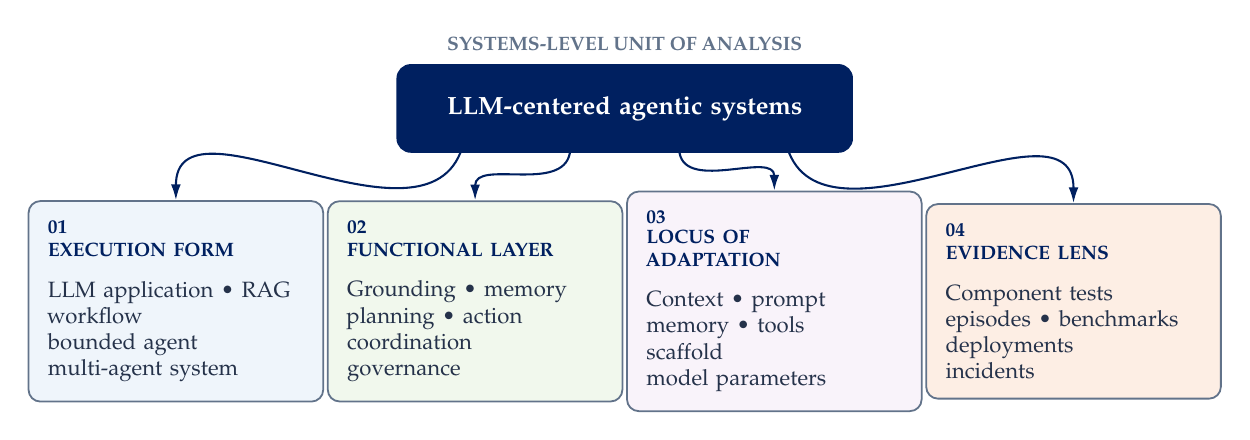
\begin{tikzpicture}[
  font=\small,
  line cap=round,
  line join=round,
  card/.style={
    rounded corners=1.5mm,
    draw=surveyLine,
    line width=0.65pt,
    align=left,
    minimum height=2.05cm,
    text width=3.25cm,
    inner xsep=7pt,
    inner ysep=7pt,
    text=surveyInk,
    font=\footnotesize
  },
  root/.style={
    rounded corners=1.7mm,
    draw=surveyNavy,
    fill=surveyNavy,
    text=white,
    line width=0.75pt,
    align=center,
    minimum height=1.10cm,
    text width=5.35cm,
    inner sep=6pt,
    font=\small\bfseries
  },
  connector/.style={
    -{Latex[length=2.0mm,width=1.25mm]},
    line width=0.75pt,
    draw=surveyNavy
  },
  eyebrow/.style={font=\scriptsize\bfseries,text=surveyNavy,align=left}
]

\node[font=\scriptsize\bfseries,text=surveyLine] at (0,0.82)
  {SYSTEMS-LEVEL UNIT OF ANALYSIS};
\node[root] (umbrella) at (0,0) {LLM-centered agentic systems};

\node[card, fill=surveyBlue!16] (forms) at (-5.7,-2.45) {
  {\color{surveyNavy}\scriptsize\bfseries 01}\\[-1pt]
  {\color{surveyNavy}\scriptsize\bfseries EXECUTION FORM}\\[5pt]
  LLM application \textbullet{} RAG\\
  workflow\\
  bounded agent\\
  multi-agent system
};

\node[card, fill=surveyGreen!16] (layers) at (-1.9,-2.45) {
  {\color{surveyNavy}\scriptsize\bfseries 02}\\[-1pt]
  {\color{surveyNavy}\scriptsize\bfseries FUNCTIONAL LAYER}\\[5pt]
  Grounding \textbullet{} memory\\
  planning \textbullet{} action\\
  coordination\\
  governance
};

\node[card, fill=surveyPurple!16] (change) at (1.9,-2.45) {
  {\color{surveyNavy}\scriptsize\bfseries 03}\\[-1pt]
  {\color{surveyNavy}\scriptsize\bfseries LOCUS OF\\[-1pt] ADAPTATION}\\[5pt]
  Context \textbullet{} prompt\\
  memory \textbullet{} tools\\
  scaffold\\
  model parameters
};

\node[card, fill=surveyOrange!13] (evidence) at (5.7,-2.45) {
  {\color{surveyNavy}\scriptsize\bfseries 04}\\[-1pt]
  {\color{surveyNavy}\scriptsize\bfseries EVIDENCE LENS}\\[5pt]
  Component tests\\
  episodes \textbullet{} benchmarks\\
  deployments\\
  incidents
};

% Four explicit ports make each dimension a direct child of the umbrella term.
% The distinct curves preserve hierarchy without a visually ambiguous bus.
\path (umbrella.south west) -- (umbrella.south east)
  coordinate[pos=.14] (portforms)
  coordinate[pos=.38] (portlayers)
  coordinate[pos=.62] (portchange)
  coordinate[pos=.86] (portevidence);
\draw[connector] (portforms) to[out=-112,in=90] (forms.north);
\draw[connector] (portlayers) to[out=-100,in=90] (layers.north);
\draw[connector] (portchange) to[out=-80,in=90] (change.north);
\draw[connector] (portevidence) to[out=-68,in=90] (evidence.north);

\end{tikzpicture}

\caption{Umbrella taxonomy used in this survey. Following the umbrella-first organizing logic used to map self-improving agents by update substrate and evaluation target~\cite{ren2026selfimprovingagents}, we place the broader literature under \emph{LLM-centered agentic systems} and compare work along four independent dimensions. The dimensions avoid treating RAG, workflows, and agents as a single maturity ladder.}
\label{fig:systems-progression}
\end{figure*}

These dimensions are compositional rather than chronological. Reliable systems are usually hybrid. A bounded agent may use a deterministic workflow for high-risk steps, a symbolic planner for constrained subproblems, RAG for evidence, and a human approval gate before committing an irreversible action. The appropriate architecture depends on task uncertainty, the cost of errors, environmental dynamics, and the availability of objective verification.

\subsection{Positioning relative to related surveys}
\label{sec:related-surveys}

Existing surveys offer complementary views: broad reviews organize agent capabilities and applications~\cite{wang2024autonomousagentssurvey,xi2025agentsurvey,plaat2025agenticllms}, while focused reviews cover RAG~\cite{gao2023ragsurvey,singh2025agenticragsurvey}, memory~\cite{zhang2025memorysurvey}, tool learning~\cite{shi2025toollearning}, evaluation~\cite{yehudai2026agentsurveyeval}, or self-improvement~\cite{ren2026selfimprovingagents}. Their root terms are not interchangeable: self-improving agents update model parameters or scaffolds from feedback, whereas many RAG, workflow, and bounded-agent systems remain fixed between episodes. \Cref{tab:related-surveys} makes the distinction explicit.

\begin{table*}[t]
\centering
\caption{Positioning against representative surveys. Primary denotes the organizing lens rather than every topic mentioned by a paper.}
\label{tab:related-surveys}
\small
\surveytableformat
\begin{tabularx}{\textwidth}{L{3.0cm}L{3.1cm}L{3.5cm}Y}
\toprule
\rowcolor{surveyBlue!28}\textbf{Survey} & \textbf{Umbrella or root term} & \textbf{Primary organizing lens} & \textbf{Relationship to this survey} \\
\midrule
Gao et al.~\cite{gao2023ragsurvey} & Retrieval-augmented generation & Naive, advanced, and modular retrieval pipelines & Deep grounding coverage; limited treatment of action authority, multi-agent coordination, and governance \\
Wang et al.~\cite{wang2024autonomousagentssurvey} & LLM-based autonomous agents & Construction, applications, and evaluation & Broad agent overview; less emphasis on cross-layer reliability contracts and operational boundaries \\
Xi et al.~\cite{xi2025agentsurvey} & LLM-based agents & Brain, perception, action, and application domains & Comprehensive capability view; RAG-to-workflow boundaries and governance are not the central lens \\
Zhang et al.~\cite{zhang2025memorysurvey} & LLM-based agent memory & Memory sources, forms, operations, and evaluation & Deep memory coverage used here as one layer within a larger systems architecture \\
Shi et al.~\cite{shi2025toollearning} & Automatic tool agents & Tool discovery, learning, selection, and use & Deep tool learning coverage; does not by itself integrate memory, governance, or deployment evidence \\
Yehudai et al.~\cite{yehudai2026agentsurveyeval} & LLM agent evaluation & Benchmarks, metrics, and evaluation protocols & Deep evaluation treatment; this survey connects evaluation to architecture and action authority \\
Ren et al.~\cite{ren2026selfimprovingagents} & Self-improving agents & Foundation model versus scaffold improvement & Provides the umbrella-first taxonomic inspiration; its scope begins where feedback changes the model or scaffold \\
\textbf{This survey} & \textbf{LLM-centered agentic systems} & \textbf{Execution form, six functional layers, adaptation locus, and evidence} & \textbf{Integrates RAG, workflows, agents, evaluation, and governance through bounded system authority} \\
\bottomrule
\end{tabularx}
\end{table*}

The overview in \Cref{fig:literature-atlas} turns this broad scope into a navigable map. It assigns 98 representative sources to one primary locus in the survey taxonomy, while the text and comparative tables interpret the larger literature and its cross-cutting contributions.

\begin{figure*}[p]
\centering
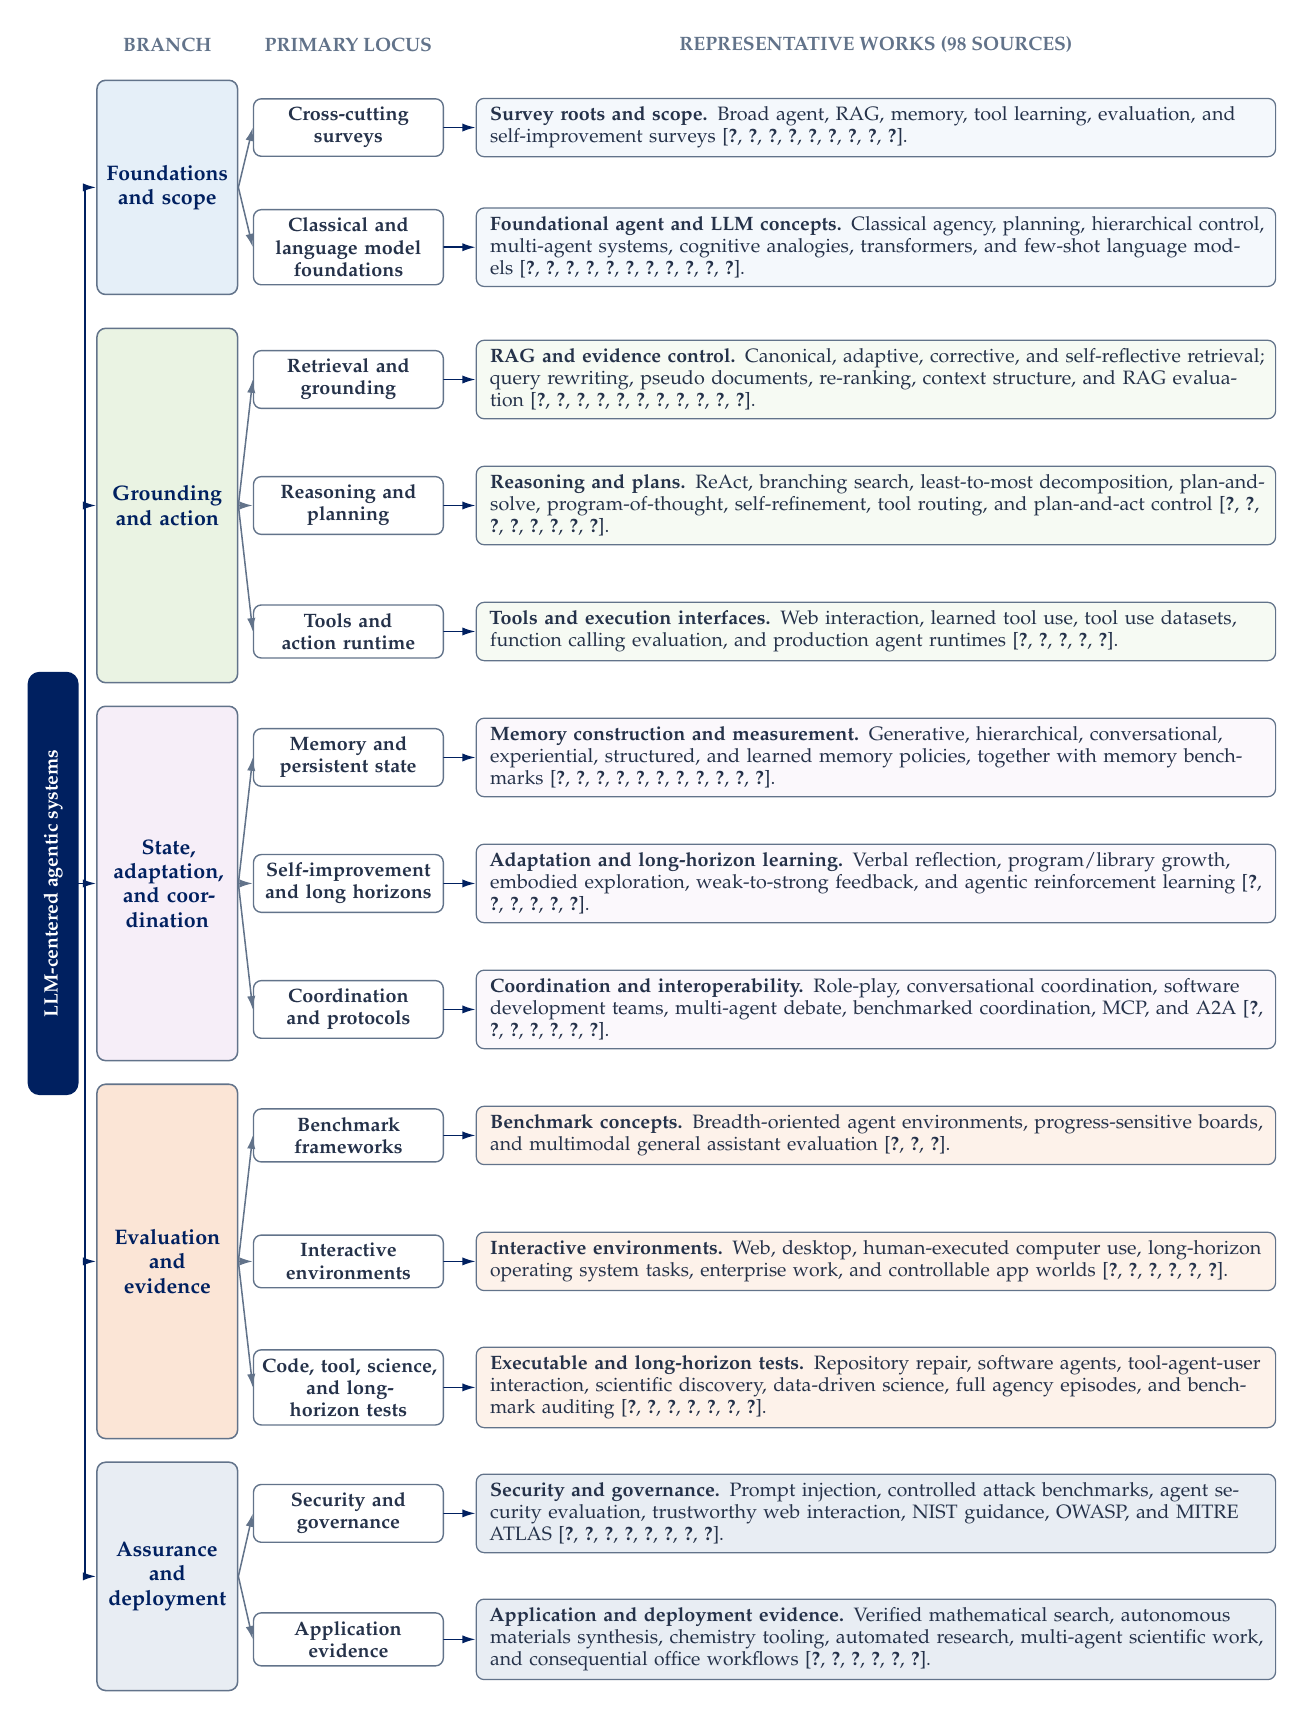
\begin{tikzpicture}[
  font=\scriptsize,
  line cap=round,
  line join=round,
  arrow/.style={
    -{Latex[length=1.7mm,width=1.05mm]},
    line width=0.55pt,
    draw=surveyLine
  },
  rootarrow/.style={arrow,line width=0.65pt,draw=surveyNavy},
  brancharrow/.style={arrow,line width=0.55pt,draw=surveyLine},
  workarrow/.style={arrow,line width=0.62pt,draw=surveyNavy},
  branch/.style={
    rounded corners=1.1mm,
    draw=surveyLine,
    line width=0.55pt,
    align=center,
    text width=1.54cm,
    inner xsep=3.5pt,
    inner ysep=5pt,
    font=\fontsize{7.6}{8.8}\selectfont\bfseries,
    text=surveyNavy
  },
  leaf/.style={
    rounded corners=1.0mm,
    draw=surveyLine,
    line width=0.5pt,
    fill=white,
    align=center,
    text width=2.20cm,
    inner xsep=3pt,
    inner ysep=3pt,
    font=\scriptsize\bfseries,
    text=surveyInk
  },
  works/.style={
    rounded corners=1.0mm,
    draw=surveyLine,
    line width=0.45pt,
    align=left,
    text width=9.80cm,
    inner xsep=5pt,
    inner ysep=3pt,
    font=\scriptsize,
    text=surveyInk
  }
]

% Column headers
\node[font=\scriptsize\bfseries,text=surveyLine] at (-6.25,1.05) {BRANCH};
\node[font=\scriptsize\bfseries,text=surveyLine] at (-3.95,1.05) {PRIMARY LOCUS};
\node[font=\scriptsize\bfseries,text=surveyLine] at (2.75,1.05) {REPRESENTATIVE WORKS (98 SOURCES)};

% Compact umbrella node and tree spine
\node[
  rounded corners=1.4mm,
  fill=surveyNavy,
  draw=surveyNavy,
  line width=0.75pt,
  minimum width=0.62cm,
  minimum height=5.35cm,
  inner sep=0pt
] (root) at (-7.70,-9.60) {};
\node[rotate=90,font=\scriptsize\bfseries,text=white,align=center]
  at (root.center) {LLM-centered agentic systems};

% Branches
\node[branch,fill=surveyBlue!26,minimum height=2.72cm] (b1) at (-6.25,-0.76)
  {Foundations\\and scope};
\node[branch,fill=surveyGreen!25,minimum height=4.50cm] (b2) at (-6.25,-4.80)
  {Grounding\\and action};
\node[branch,fill=surveyPurple!23,minimum height=4.50cm] (b3) at (-6.25,-9.60)
  {State, adaptation,\\and coordination};
\node[branch,fill=surveyOrange!20,minimum height=4.50cm] (b4) at (-6.25,-14.40)
  {Evaluation\\and evidence};
\node[branch,fill=surveyMuted,minimum height=2.90cm] (b5) at (-6.25,-18.40)
  {Assurance\\and deployment};

% Primary loci
\node[leaf] (l1) at (-3.95,0.00) {Cross-cutting\\surveys};
\node[leaf] (l2) at (-3.95,-1.52) {Classical and\\language model foundations};
\node[leaf] (l3) at (-3.95,-3.20) {Retrieval and\\grounding};
\node[leaf] (l4) at (-3.95,-4.80) {Reasoning and\\planning};
\node[leaf] (l5) at (-3.95,-6.40) {Tools and\\action runtime};
\node[leaf] (l6) at (-3.95,-8.00) {Memory and\\persistent state};
\node[leaf] (l7) at (-3.95,-9.60) {Self-improvement\\and long horizons};
\node[leaf] (l8) at (-3.95,-11.20) {Coordination\\and protocols};
\node[leaf] (l9) at (-3.95,-12.80) {Benchmark\\frameworks};
\node[leaf] (l10) at (-3.95,-14.40) {Interactive\\environments};
\node[leaf] (l11) at (-3.95,-16.00) {Code, tool, science,\\and long-horizon tests};
\node[leaf] (l12) at (-3.95,-17.60) {Security and\\governance};
\node[leaf] (l13) at (-3.95,-19.20) {Application\\evidence};

% Literature leaves. Each mapped source is deliberately assigned once.
\node[works,fill=surveyBlue!11] (w1) at (2.75,0.00) {\textbf{Survey roots and scope.} Broad agent, RAG, memory, tool learning, evaluation, and self-improvement surveys~\cite{wang2024autonomousagentssurvey,xi2025agentsurvey,plaat2025agenticllms,ren2026selfimprovingagents,gao2023ragsurvey,singh2025agenticragsurvey,zhang2025memorysurvey,shi2025toollearning,yehudai2026agentsurveyeval}.};
\node[works,fill=surveyBlue!11] (w2) at (2.75,-1.52) {\textbf{Foundational agent and LLM concepts.} Classical agency, planning, hierarchical control, multi-agent systems, cognitive analogies, transformers, and few-shot language models~\cite{russell2021aima,rao1995bdi,wooldridge2009multiagent,kaelbling1998pomdp,sutton1999options,fikes1971strips,erol1994htn,mcdermott1998pddl,hawkins2021thousandbrains,vaswani2017attention,brown2020language}.};
\node[works,fill=surveyGreen!11] (w3) at (2.75,-3.20) {\textbf{RAG and evidence control.} Canonical, adaptive, corrective, and self-reflective retrieval; query rewriting, pseudo documents, re-ranking, context structure, and RAG evaluation~\cite{lewis2020rag,ghodratnama2024adapting,ma2023queryrewriting,wang2023query2doc,shi2023replug,jiang2023flare,asai2024selfrag,sarthi2024raptor,yan2024crag,es2024ragas,liu2024lostinthemiddle}.};
\node[works,fill=surveyGreen!11] (w4) at (2.75,-4.80) {\textbf{Reasoning and plans.} ReAct, branching search, least-to-most decomposition, plan-and-solve, program-of-thought, self-refinement, tool routing, and plan-and-act control~\cite{yao2023react,yao2023treeofthoughts,zhou2023leasttomost,wang2023planandsolve,chen2023pot,madaan2023selfrefine,karpas2022mrkl,erdogan2025planandact}.};
\node[works,fill=surveyGreen!11] (w5) at (2.75,-6.40) {\textbf{Tools and execution interfaces.} Web interaction, learned tool use, tool use datasets, function calling evaluation, and production agent runtimes~\cite{nakano2021webgpt,schick2023toolformer,qin2024toolllm,openai2025agentssdk,patil2025bfcl}.};
\node[works,fill=surveyPurple!10] (w6) at (2.75,-8.00) {\textbf{Memory construction and measurement.} Generative, hierarchical, conversational, experiential, structured, and learned memory policies, together with memory benchmarks~\cite{park2023generativeagents,packer2024memgpt,zhong2024memorybank,zhao2024expel,xu2025amem,chhikara2025mem0,yu2026agemem,ghodratnama2023personalized,ghodratnama2024sumrecom,tan2025membench,shen2026mem2actbench}.};
\node[works,fill=surveyPurple!10] (w7) at (2.75,-9.60) {\textbf{Adaptation and long-horizon learning.} Verbal reflection, program/library growth, embodied exploration, weak-to-strong feedback, and agentic reinforcement learning~\cite{shinn2023reflexion,gao2023pal,wang2023voyager,li2026soar,lu2026supo,zakershahrak2024explanation}.};
\node[works,fill=surveyPurple!10] (w8) at (2.75,-11.20) {\textbf{Coordination and interoperability.} Role-play, conversational coordination, software development teams, multi-agent debate, benchmarked coordination, MCP, and A2A~\cite{li2023camel,wu2023autogen,hong2024metagpt,du2024multiagentdebate,zhu2025multiagentbench,mcp2025spec,a2a2026spec}.};
\node[works,fill=surveyOrange!10] (w9) at (2.75,-12.80) {\textbf{Benchmark concepts.} Breadth-oriented agent environments, progress-sensitive boards, and multimodal general assistant evaluation~\cite{liu2024agentbench,hsieh2024agentboard,mialon2024gaia}.};
\node[works,fill=surveyOrange!10] (w10) at (2.75,-14.40) {\textbf{Interactive environments.} Web, desktop, human-executed computer use, long-horizon operating system tasks, enterprise work, and controllable app worlds~\cite{zhou2024webarena,xie2024osworld,abhyankar2025osworldhuman,yuan2026osworld2,drouin2024workarena,trivedi2024appworld}.};
\node[works,fill=surveyOrange!10] (w11) at (2.75,-16.00) {\textbf{Executable and long-horizon tests.} Repository repair, software agents, tool-agent-user interaction, scientific discovery, data-driven science, full agency episodes, and benchmark auditing~\cite{jimenez2024swebench,yang2024sweagent,yao2024taubench,jansen2024discoveryworld,chen2025scienceagentbench,li2026agencybench,openai2026swebenchaudit}.};
\node[works,fill=surveyMuted] (w12) at (2.75,-17.60) {\textbf{Security and governance.} Prompt injection, controlled attack benchmarks, agent security evaluation, trustworthy web interaction, NIST guidance, OWASP, and MITRE ATLAS~\cite{greshake2023promptinjection,zhan2024injecagent,zhang2024agentsecuritybench,levy2026stwebagentbench,nist2023airmf,nist2024genaiprofile,owasp2025llmtop10,mitre2026atlas}.};
\node[works,fill=surveyMuted] (w13) at (2.75,-19.20) {\textbf{Application and deployment evidence.} Verified mathematical search, autonomous materials synthesis, chemistry tooling, automated research, multi-agent scientific work, and consequential office workflows~\cite{romeraparedes2024funsearch,szymanski2023alab,bran2024chemcrow,lu2024aiscientist,ghafarollahi2024sciagents,xu2025agentcompany}.};

% Root-to-branch and branch-to-leaf hierarchy.
\draw[draw=surveyNavy,line width=0.65pt] (root.east) -- (-7.30,-9.60);
\draw[draw=surveyNavy,line width=0.65pt] (-7.30,-18.40) -- (-7.30,-0.76);
\foreach \branch/\y in {b1/-.76,b2/-4.80,b3/-9.60,b4/-14.40,b5/-18.40}
  \draw[rootarrow] (-7.30,\y) -- (\branch.west);
\foreach \leaf in {l1,l2}
  \draw[brancharrow] (b1.east) -- (\leaf.west);
\foreach \leaf in {l3,l4,l5}
  \draw[brancharrow] (b2.east) -- (\leaf.west);
\foreach \leaf in {l6,l7,l8}
  \draw[brancharrow] (b3.east) -- (\leaf.west);
\foreach \leaf in {l9,l10,l11}
  \draw[brancharrow] (b4.east) -- (\leaf.west);
\foreach \leaf in {l12,l13}
  \draw[brancharrow] (b5.east) -- (\leaf.west);
\foreach \leaf/\work in {l1/w1,l2/w2,l3/w3,l4/w4,l5/w5,l6/w6,l7/w7,l8/w8,l9/w9,l10/w10,l11/w11,l12/w12,l13/w13}
  \draw[workarrow] (\leaf.east) -- (\work.west);
\end{tikzpicture}

\caption{Comprehensive literature taxonomy for LLM-centered agentic systems. Inspired by the umbrella-first, work-level mapping in the self-improvement survey of Ren et al.~\cite{ren2026selfimprovingagents}, this atlas assigns 98 representative sources to one primary locus. The placement expresses the source's principal contribution, not an exclusive claim: many methods span multiple layers, and the surrounding text and tables cover additional work.}
\label{fig:literature-atlas}
\end{figure*}

\subsection{Scope and literature selection}
\label{sec:survey-method}

This systems-oriented narrative survey covers LLM-centered agentic systems through \reviewcutoff across the execution forms and functional layers in \Cref{fig:systems-progression}; it does not claim to enumerate every implementation. We synthesize peer-reviewed research, public benchmarks, influential preprints where mature coverage is unavailable, and official specifications for evolving protocols. Included work contributes materially to grounding, architecture, state, planning, tools, coordination, adaptation, evaluation, safety, interoperability, or deployment. Ordinary chat and fixed pipelines appear only when they clarify a boundary, and vendor deployments are treated as case studies rather than independent evidence of general effectiveness.

Because products and leaderboards change quickly, we emphasize durable abstractions and benchmark methodology: frameworks are compared by control and operational guarantees, and results expose capability gaps rather than declare permanent rankings.

\subsection{Contributions and organization}

The survey makes the following contributions:

\begin{itemize}
    \item \textbf{An umbrella term and operational definitions.} We use LLM-centered agentic systems for the broader systems family, then distinguish LLM applications, RAG, deterministic workflows, bounded agents, and multi-agent systems by control, state, and action authority.
    \item \textbf{A multidimensional systems taxonomy.} We compare execution form, six functional layers, locus of adaptation, and evidence rather than presenting RAG, workflows, and agents as a single maturity ladder.
    \item \textbf{Integrated foundations and current mechanisms.} We connect classical agency and planning to modern RAG, memory policies, long-horizon learning, MCP, and A2A.
    \item \textbf{Comparative evidence and deployment guidance.} We map mechanisms, benchmarks, safety sources, and application studies to the claims they support, then connect outcome, trajectory, cost, recovery, and side effect metrics to typed contracts, least privilege, approval, verification, tracing, and replay.
\end{itemize}

The review follows one systems narrative: RAG moves from grounding a response to deciding when to seek evidence; foundations explain state, planning, uncertainty, and bounded action; architecture turns them into memory, decision, tool, and coordination components; evaluation asks what can justify a capability claim; and governance and applications test whether that claim survives consequential deployment. The final sections identify open problems along the same evidence-to-action-to-accountability path.

\section{Retrieval-Augmented Generation and the Transition to Agentic Retrieval}
\label{sec:rag}

Retrieval-Augmented Generation (RAG) is the first point in this survey at which external information becomes explicit system state rather than remaining implicit in model parameters or transient prompting. In its canonical form, a retriever maps a query to passages from an external corpus and a generator conditions on the query and those passages to produce an answer~\cite{lewis2020rag}. The systems consequence is more important than the pipeline shorthand: each retrieved passage can be represented as an evidence object carrying content, source identity and version, retrieval time, access scope, score, and provenance, then persisted with the claims it is used to support. This boundary makes frequently changing or access-controlled knowledge replaceable and auditable without retraining the model. It does not make a retrieved passage true, nor does it grant the model action authority; it makes the available support inspectable. The model is therefore a synthesis and decision component operating over a bounded evidence record, while the external collection remains the attributable source.

The familiar four-stage summary (indexing, retrieval, context construction, and generation) hides the state transformations that make RAG dependable. Indexing creates addressable, versioned evidence units; retrieval selects candidates under a query and access policy; context construction normalizes, reranks, deduplicates, and assigns evidence identifiers; generation consumes that bounded record; and post-generation verification maps claims back to supporting items. Production systems therefore add ingestion controls, access filtering, ranking, citation mapping, caching, monitoring, and verification. Because the retrieval layer may combine sparse lexical search, dense vectors, graph traversal, structured queries, or external search APIs, RAG is a family of architectures whose choices determine which evidence and metadata the system can represent~\cite{gao2023ragsurvey}. Work on LLM-mediated information retrieval reaches the same systems conclusion: retrieval quality is coupled to model selection, orchestration, scaling cost, privacy, interpretability, and personalization~\cite{ghodratnama2024adapting}. A retrieval metric cannot therefore be interpreted in isolation; the pipeline must preserve provenance and access constraints and expose its transformations as inspectable state transitions.


\begin{figure*}[!t]
\centering
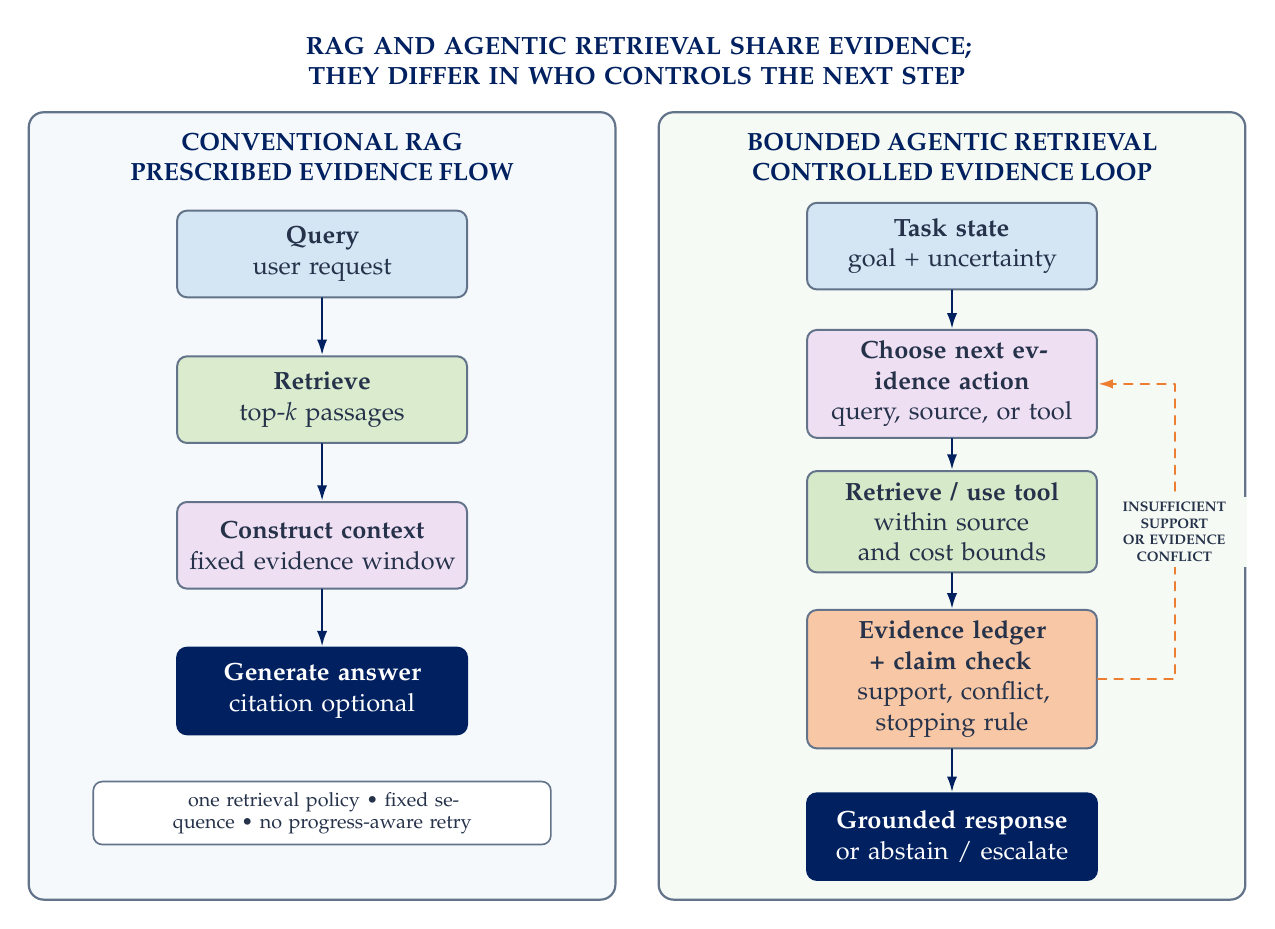
\begin{tikzpicture}[
  font=\small,
  line cap=round,
  line join=round,
  pane/.style={
    rounded corners=1.9mm,
    draw=surveyLine,
    line width=0.8pt,
    fill=white
  },
  block/.style={
    rounded corners=1.25mm,
    draw=surveyLine,
    line width=0.72pt,
    align=center,
    text width=34mm,
    minimum height=11mm,
    inner sep=4pt,
    text=surveyInk
  },
  arr/.style={
    -{Latex[length=2.0mm,width=1.3mm]},
    line width=0.9pt,
    draw=surveyNavy
  },
  feedback/.style={
    -{Latex[length=1.9mm,width=1.2mm]},
    line width=0.85pt,
    dashed,
    draw=surveyOrange
  },
  note/.style={
    rounded corners=1.15mm,
    draw=surveyLine,
    line width=0.6pt,
    fill=white,
    align=center,
    text width=56mm,
    minimum height=8mm,
    inner sep=3pt,
    font=\scriptsize,
    text=surveyInk
  }
]

\node[font=\small\bfseries,text=surveyNavy,align=center,text width=15.0cm] at (0,2.00)
  {RAG AND AGENTIC RETRIEVAL SHARE EVIDENCE;\\
   THEY DIFFER IN WHO CONTROLS THE NEXT STEP};

% A readable side-by-side comparison: the action sequence stays vertical, and
% only the bounded system is allowed to decide what evidence work comes next.
\node[pane,fill=surveyBlue!10,minimum width=7.45cm,minimum height=10.00cm] at (-4.00,-3.65) {};
\node[font=\small\bfseries,text=surveyNavy,align=center] at (-4.00,0.78)
  {CONVENTIONAL RAG\\PRESCRIBED EVIDENCE FLOW};
\node[block,fill=surveyBlue!43] (q) at (-4.00,-0.45) {\textbf{Query}\\user request};
\node[block,fill=surveyGreen!43] (retrieve) at (-4.00,-2.30) {\textbf{Retrieve}\\top-$k$ passages};
\node[block,fill=surveyPurple!43] (context) at (-4.00,-4.15) {\textbf{Construct context}\\fixed evidence window};
\node[block,fill=surveyNavy,draw=surveyNavy,text=white] (answer) at (-4.00,-6.00) {\textbf{Generate answer}\\citation optional};
\draw[arr] (q.south) -- (retrieve.north);
\draw[arr] (retrieve.south) -- (context.north);
\draw[arr] (context.south) -- (answer.north);
\node[note] at (-4.00,-7.55)
  {one retrieval policy \textbullet{} fixed sequence \textbullet{} no progress-aware retry};

\node[pane,fill=surveyGreen!10,minimum width=7.45cm,minimum height=10.00cm] at (4.00,-3.65) {};
\node[font=\small\bfseries,text=surveyNavy,align=center] at (4.00,0.78)
  {BOUNDED AGENTIC RETRIEVAL\\CONTROLLED EVIDENCE LOOP};
\node[block,fill=surveyBlue!43] (state) at (4.00,-0.35) {\textbf{Task state}\\goal + uncertainty};
\node[block,fill=surveyPurple!43] (plan) at (4.00,-2.10) {\textbf{Choose next evidence action}\\query, source, or tool};
\node[block,fill=surveyGreen!48] (search) at (4.00,-3.85) {\textbf{Retrieve / use tool}\\within source and cost bounds};
\node[block,fill=surveyOrange!43] (check) at (4.00,-5.85) {\textbf{Evidence ledger + claim check}\\support, conflict, stopping rule};
\node[block,fill=surveyNavy,draw=surveyNavy,text=white] (response) at (4.00,-7.85) {\textbf{Grounded response}\\or abstain / escalate};
\draw[arr] (state.south) -- (plan.north);
\draw[arr] (plan.south) -- (search.north);
\draw[arr] (search.south) -- (check.north);
\draw[arr] (check.south) -- (response.north);
\draw[feedback] (check.east) -- ++(0.98,0) |- (plan.east);
\node[fill=surveyGreen!10,inner sep=2pt,
  font=\tiny\bfseries,text=surveyInk,align=center,text width=17mm]
  at (6.82,-3.98) {INSUFFICIENT SUPPORT\\OR EVIDENCE CONFLICT};

\end{tikzpicture}

\caption{Conventional RAG and bounded agentic retrieval share an evidence pipeline but not a control model. Conventional RAG executes a prescribed retrieval sequence. Bounded agentic retrieval preserves task and evidence state, chooses retrieval actions inside an explicit authority boundary, and uses support or conflict to re-plan, abstain, or escalate. The additional loop is justified only when those decisions are observable and governed.}
\label{fig:agentic-rag}
\end{figure*}

\subsection{Why RAG is useful and what it does not guarantee}

RAG's four recurring advantages all follow from externalizing evidence. An evidence store can be refreshed without retraining the base model; retrieval can enforce scope and access policy before content enters model context; passage identifiers and document versions can support citation and audit; and domain-specific corpora can improve task performance without full model adaptation. None of these properties makes the resulting answer true. Failures arise at distinct layers: retrieval can return irrelevant, stale, duplicated, or unauthorized items; representation can omit provenance or access metadata; context use can fail when the model overlooks relevant passages, especially in long contexts~\cite{liu2024lostinthemiddle}; and retrieved content can carry adversarial instructions across the trust boundary~\cite{greshake2023promptinjection}. Even an intact citation establishes association, not entailment of the attached claim. RAGAS-style evaluation therefore separates context relevance, answer relevance, and faithfulness rather than treating retrieval success as a single score~\cite{es2024ragas}. RAG reduces reliance on parametric memory and makes support auditable, but it does not provide a factuality guarantee; downstream control still needs explicit support, conflict, abstention, and stopping states.

Evaluating RAG as an evidence-to-claim transformation requires three questions and three corresponding records:
\begin{enumerate}
    \item \textbf{Evidence discovery}: Does the retrieval record contain sufficient relevant information from permissible sources, together with the query, source version, rank, and retrieval metadata needed to explain the selection?
    \item \textbf{Evidence use}: Does the generation trace show that the model correctly interpreted the retrieved information, resolved or exposed conflicts, and carried relevant uncertainty into the answer?
    \item \textbf{Claim support}: Can each externally verifiable claim be linked to identifiable evidence that entails it, or be explicitly marked unsupported and handled through abstention or further search?
\end{enumerate}
The three levels are causally ordered but not interchangeable. A correct answer may come from parametric memory despite failed retrieval; a high-quality context may be ignored or misinterpreted; and correctly used evidence may still fail to entail the final wording of a claim. Evaluation should therefore report the levels separately and retain their artifacts for attribution and replay, so improvement at one layer cannot conceal regression at another.

\subsection{Evolution of RAG architectures}

The familiar progression from naive to advanced, modular, and agentic RAG is useful only when read as a relocation of control rather than a maturity ladder. Naive RAG fixes the retrieve--construct--generate sequence; advanced RAG improves one or more transformations inside that sequence; modular RAG exposes retrieval, ranking, synthesis, and verification as composable components; and agentic RAG allows a controller to select the next evidence action from explicit task and evidence state~\cite{gao2023ragsurvey,singh2025agenticragsurvey}. The categories overlap, and production systems are often hybrid. We therefore compare them along three operational axes: who selects the next retrieval transition, which evidence and intermediate state persist, and which stopping and verification boundaries constrain the result.

\paragraph{Naive RAG.}
Naive RAG fixes the evidence policy: encode one query, retrieve top-$k$ passages, construct context, and generate~\cite{lewis2020rag}. This path is inexpensive and auditable for narrow questions over stable corpora, but it cannot revise the source, query, or stopping decision when evidence is weak. Query wording, chunking, and context position therefore remain consequential failure points~\cite{liu2024lostinthemiddle}. Naive RAG is a fixed workflow, not a primitive agent.

\paragraph{Advanced RAG.}
Advanced RAG keeps a developer-authored flow while improving query, candidate, or context transformations. Rewriting and pseudo document expansion change the represented information need~\cite{ma2023queryrewriting,wang2023query2doc}; REPLUG adapts retrieval around a black-box model~\cite{shi2023replug}; and FLARE and Self-RAG condition retrieval on uncertainty or learned critique~\cite{jiang2023flare,asai2024selfrag}. These mechanisms make evidence acquisition responsive, but the enclosing system remains an adaptive workflow when its branches and authority are fixed in advance.

\paragraph{Modular RAG.}
Modular RAG exposes routing, retrieval, ranking, context construction, synthesis, and verification as components with typed artifacts. RAPTOR adds multi-resolution retrieval~\cite{sarthi2024raptor}, while Corrective RAG represents relevance and invokes fallback search when local evidence is weak~\cite{yan2024crag}. Modularity localizes evaluation and supports heterogeneous sources, but expands the contract surface for schemas, freshness, access, and provenance. A developer-authored routing graph is still a workflow; its importance is that it creates inspectable state surfaces on which bounded control can operate.

\paragraph{Agentic RAG.}
Agentic RAG moves selection of the next evidence transition to a controller that can rewrite, change source, inspect conflict, request clarification, or abstain from explicit task and evidence state. ReAct illustrates how observations can revise subsequent action~\cite{yao2023react}, and Agentic RAG generalizes that pattern to iterative evidence acquisition~\cite{singh2025agenticragsurvey}. The benefit is adaptive multi-hop search; the cost is looping, noisy evidence overfitting, boundary crossing, and indirect prompt injection~\cite{greshake2023promptinjection}. Agentic retrieval is therefore bounded evidence action under permissions, budgets, stopping rules, and traceable state.

\begin{table*}[t]
\centering
\caption{Comparison of representative retrieval-augmented architectures. The rows describe dominant tendencies rather than strict implementation requirements.}
\label{tab:rag-evolution}
\small
\surveytableformat
\begin{tabularx}{\textwidth}{L{2.3cm}Y Y Y Y}
\toprule
\rowcolor{surveyBlue!28}\textbf{Architecture} & \textbf{Retrieval policy} & \textbf{Control flow} & \textbf{Primary strength} & \textbf{Characteristic risk} \\
\midrule
Naive RAG & One top-$k$ query over a fixed index & Fixed retrieve--generate pipeline & Simplicity and low latency & Query mismatch and unsupported synthesis \\
Advanced RAG & Rewriting, hybrid search, re-ranking, or iterative retrieval & Mostly developer-defined & Better evidence recall and precision & Pipeline complexity and evaluation leakage between stages \\
Modular RAG & Source routing and task-specific retrieval modules & Explicit graph or state machine & Inspectability and heterogeneous evidence access & Configuration burden and inconsistent component contracts \\
Agentic RAG & Model- or policy-selected retrieval actions & Adaptive observe--retrieve--reason--verify loop & Multi-hop search and uncertainty-driven evidence collection & Runaway search, adversarial content, and non-reproducible trajectories \\
\bottomrule
\end{tabularx}
\end{table*}

\begin{table*}[t]
\centering
\caption{Representative RAG mechanisms and the evidence each isolates. Reported improvements are not directly comparable because tasks, corpora, generators, and retrieval budgets differ.}
\label{tab:rag-method-evidence}
\small
\surveytableformat
\begin{tabularx}{\textwidth}{L{2.55cm}L{3.05cm}L{3.15cm}Y}
\toprule
\rowcolor{surveyBlue!28}\textbf{Method} & \textbf{Mechanism changed} & \textbf{Evaluation focus} & \textbf{Systems implication and limitation} \\
\midrule
Query2doc~\cite{wang2023query2doc} & Generates a pseudo document to expand the query & Retrieval effectiveness across standard search datasets & Improves query representation, but added generated text can introduce unsupported terms \\
Query rewriting~\cite{ma2023queryrewriting} & Rewrites the user request before retrieval & Downstream QA and retrieval quality & Separates intent interpretation from retrieval, but relies on rewrite faithfulness \\
REPLUG~\cite{shi2023replug} & Trains or weights a retriever around a frozen black-box LM & Language model and knowledge-intensive tasks & Supports model-agnostic retrieval; does not supply an agent control loop \\
FLARE~\cite{jiang2023flare} & Triggers retrieval during generation from anticipated uncertainty & Long-form knowledge-intensive generation & Demonstrates adaptive retrieval, but retrieval policy and generation quality remain coupled \\
RAPTOR~\cite{sarthi2024raptor} & Retrieves over a tree of recursively summarized clusters & Multi-step question answering over long corpora & Adds multi-resolution evidence access; summaries create additional lineage and fidelity obligations \\
Self-RAG~\cite{asai2024selfrag} & Learns retrieve, relevance, support, and utility reflection tokens & Factuality and task performance across QA and generation & Integrates retrieval decisions with generation; requires trained reflection behavior \\
Corrective RAG~\cite{yan2024crag} & Scores retrieved evidence and invokes a corrective search path & Robustness to low-quality initial retrieval & Makes recovery explicit; external search broadens trust and provenance boundaries \\
RAGAS~\cite{es2024ragas} & Decomposes evaluation into faithfulness and context-related metrics & Reference-light RAG evaluation & Enables component diagnosis, but judge-based metrics require calibration against humans \\
\bottomrule
\end{tabularx}
\end{table*}

\subsection{Data, indexing, and freshness}

The quality of a RAG system is bounded before the first query is issued. Ingestion converts a source document into persistent, typed evidence records; each record should retain document identity and version, timestamps, ownership, access policy, lineage, and the offsets needed to reconstruct the source passage. Chunking then determines the semantic unit to which retrieval scores, citations, and later claim checks refer. Units must be small enough for discriminative retrieval but complete enough to preserve definitions, tables, code structure, and cross-references. Fixed-length chunks are operationally convenient yet can sever precisely the context needed for entailment. Structure-aware and hierarchical schemes preserve section and parent--child relations and allow local passages to remain connected to broader summaries, as illustrated by RAG architecture surveys and RAPTOR~\cite{gao2023ragsurvey,sarthi2024raptor}. Bounded action therefore begins with the data model: a later controller cannot reliably enforce freshness, authorization, or provenance that ingestion discarded.

Freshness is not merely an indexing schedule; it is a consistency property of the evidence state. Vector and lexical stores can accept incremental insertions, deletions, and replacements, but every derived object (chunk, embedding, summary, graph edge, and cache entry) must inherit the source's identity and version so that a change can invalidate its descendants. This dependency graph allows the system to distinguish current, stale, and revoked evidence and to record which version supported a later claim or action. For stable corpora, scheduled incremental maintenance may suffice; for volatile facts, evidence should instead be obtained at decision time from an authoritative database, API, or search index. FreshLLMs demonstrates why this distinction matters: models struggle on fast-changing questions, whereas retrieving current search evidence improves factuality~\cite{vu2023freshllms}; CRAG similarly invokes web search as a corrective source when local retrieval is unreliable~\cite{yan2024crag}. In the survey's terms, index maintenance is therefore not back-office plumbing: it is the temporal contract between evidence state and bounded action.

Authorization is part of evidence validity, not a filter applied to prose after generation. A passage is eligible evidence only when the requesting principal and tenant are permitted to use its source at retrieval time. Row-, document-, and tenant-level policy labels must therefore travel with the evidence record and be enforced in the retrieval query; cache keys, shared summaries, and reranking stages must preserve the same boundary. Post-generation redaction is strictly weaker because the model has already observed the material, and a retrieved instruction may redirect later tool use. Greshake et al. show that indirect prompts embedded in retrieved data can induce data theft and unauthorized API behavior~\cite{greshake2023promptinjection}, while OWASP recommends least privilege access to data sources and authorization in downstream systems rather than delegation to the model~\cite{owasp2025llmtop10}. The retrieval trace should consequently record the principal, policy version, authorization decision, and evidence objects released. This turns access control into an auditable constraint on the evidence-to-action transition.

\subsection{Context construction and evidence compression}

Retrieval produces candidates; context construction selects the evidence the model will actually see. The objective is sufficient, complementary support within a bounded context, not maximum passage count. Position effects make indiscriminate length unreliable~\cite{liu2024lostinthemiddle}; RECOMP shows that selective compression can sharply reduce context with little task loss and can omit unhelpful augmentation~\cite{xu2024recomp}. Compression is therefore an evidence transformation whose source identity, version, offsets, and lineage must remain recoverable.

Long context and retrieval solve different problems. A context window holds transient input; it does not select evidence, enforce freshness, or preserve state. Retrieval remains useful even at longer context lengths and can match substantially larger fine-tuned contexts with less computation~\cite{xu2024retrievalmeets}. Long context is therefore workspace, retrieval locates and refreshes evidence, and structured memory persists state. The design question is which information remains transient, fetched on demand, or durably retained.

\subsection{When retrieval should become agentic}

Retrieval should become agentic only when consequential evidence choices are difficult to pre-specify yet observable enough to verify. Fixed retrieval remains preferable when sources, ranking, and stopping are known. When evidence is insufficient or conflicting, an escalation ladder can permit a bounded rewrite, second source, clarification, or abstention before granting open-ended planning. FLARE and CRAG show how adaptive retrieval can sit behind explicit triggers~\cite{jiang2023flare,yan2024crag}. Each added degree of freedom should carry source, step, token, and time limits plus a stopping rule, so autonomy increases only with observability and control.

\subsection{From evidence access to closed-loop agency}

RAG solves evidence access; closed-loop agency begins when evidence can revise state and the next bounded action. ReAct and Reflexion show how observations and evaluated outcomes can alter later behavior~\cite{yao2023react,shinn2023reflexion}, but reliability requires the goal, evidence, proposal, authorization, result, and remaining uncertainty to remain explicit. Retrieval then becomes one perception mechanism within a bounded state machine that chooses among typed alternatives and verifies their postconditions. Evidence becomes operational only through that controlled transition into action.

\section{Foundations of Agentic Systems}
\label{sec:background}

The term \emph{agent} predates large language models by decades. Classical artificial intelligence defines agency through a control loop: an entity perceives an environment, maintains information relevant to an objective, and selects actions that alter what happens next~\cite{russell2021aima}; multi-agent systems additionally make autonomy, interaction, and coordination first-class concerns~\cite{wooldridge2009multiagent}. The LLM era changes the representational substrate, not this contract. Natural language can encode goals, observations, plans, tool requests, and messages, but those strings become reliable system state only when mapped into explicit, typed, and persistent records. An LLM is therefore best understood as a policy and representation transformer within an agent architecture, not as the architecture itself. A modern agentic system must preserve what was observed, which evidence was accepted, which goal is active, what action was proposed, why it was permitted, and what result followed. That data model is the bridge from evidence to bounded action. This section uses reactive control, deliberative planning, decision-making under uncertainty, hierarchical organization, and multi-agent coordination to explain which component should own each transition and under what constraints.

\subsection{An operational model of agency}

We model a bounded agent as a tuple
\begin{equation}
\mathcal{A}=\langle \mathcal{O},\mathcal{S},\mathcal{G},\mathcal{U},\pi,\mathcal{V},\mathcal{B}\rangle,
\end{equation}
The tuple separates representations from control responsibilities. $\mathcal{O}$ specifies the admissible observation and evidence types; $\mathcal{S}$ is the maintained, persistent state space; $\mathcal{G}$ contains task specifications, including success and termination criteria; and $\mathcal{U}$ defines the schemas for actions or tool calls the architecture can issue. The policy $\pi$ proposes an action from the current state and task, but it does not by itself authorize execution. $\mathcal{B}$ supplies externally enforceable bounds such as permissions, time, cost, source access, and maximum steps, while $\mathcal{V}$ evaluates the transition and determines whether to accept, repair, escalate, or terminate. For $g\in\mathcal{G}$, $\pi$ may be an LLM, a symbolic controller, a learned policy, or a composition of them. This prevents the generative component from defining evidence, state, action, authority, and outcome at once. Observations, goals, proposals, policy decisions, and outcomes must remain distinct typed records so the loop can be inspected or resumed.

\begin{samepage}
At step $t$, an observation updates state, the policy proposes an action, the bounds gate authorizes it, and the environment returns the next observation:
\begin{align}
s_t &= f(s_{t-1},o_t),\\
\tilde{u}_t &\sim \pi(\cdot\mid s_t,g,\mathcal{U}),\\
u_t &= \Gamma_{\mathcal{B}}(\tilde{u}_t,s_t),\\
o_{t+1} &\sim P_{\mathcal{E}}(\cdot\mid s_t,u_t),\\
d_t &= \mathcal{V}(s_t,\tilde{u}_t,u_t,o_{t+1}),
\end{align}
\end{samepage}
The equations separate proposal, authority, and outcome. The update function $f$ first commits the new observation to maintained state. The policy $\pi$ then emits a candidate $\tilde{u}_t$; it does not execute it. The gate $\Gamma_{\mathcal{B}}$ evaluates that proposal against the current state and operational bounds, returning either an authorized $u_t\in\mathcal{U}$ or $\bot$. The latter is a typed result rather than an exception: it records denial, abortion, a controlled no-op, or escalation. Only the authorized action reaches the environment kernel $P_{\mathcal{E}}$, whose stochastic response captures changing APIs, tools, users, and physical or digital environments. Execution success is therefore not equivalent to task success. The validator $\mathcal{V}$ compares the prior state, proposed and authorized actions, and resulting observation to produce $d_t$, such as accept, repair, escalate, or terminate. That decision and its supporting evidence should be persisted with the transition. The formulation imposes two useful invariants: no proposed action bypasses the bounds gate, and no observed outcome bypasses validation. An LLM may implement part of $\pi$ or $\mathcal{V}$, but it cannot supply these guarantees alone; agency emerges from the complete, inspectable loop.

\subsection{Reactive, deliberative, and hybrid control}

Reactive and deliberative control differ principally in how much structured state stands between observation and action. A reactive controller maps the current observation and a compact local state directly to an action. This minimizes latency and can be robust when preconditions are observable and local rules are sufficient, but it provides little machinery for aggregating evidence across time, representing delayed consequences, or comparing alternative futures. A deliberative controller instead persists a goal, an action model, and candidate future states before selecting what to do. STRIPS and PDDL make this representational requirement explicit by encoding actions as transition operators with typed preconditions and effects~\cite{fikes1971strips,mcdermott1998pddl}; BDI architectures separate beliefs, desires, and intentions, distinguishing informational state, objectives, and committed courses of action~\cite{rao1995bdi}. These are not merely historical labels. Reactive control deliberately narrows the representation and decision horizon, whereas deliberation expands both the state that must be maintained and the transitions that must be validated. The appropriate choice depends on the evidence and consequence structure of the task, not on whether an LLM is present.

Most practical LLM agents are hybrid because proposal and execution have different assurance requirements. A language model planner can interpret an underspecified goal, decompose it, and propose or revise a candidate plan; a reactive execution layer must translate each step into a typed command, check its schema, preconditions, permissions, idempotency, and budget, and commit the result to state. Toolformer demonstrates that a model can learn which API to call, when to call it, and which arguments to supply~\cite{schick2023toolformer}; ToolLLM extends tool learning evidence to single- and multi-tool solution paths over a large API collection~\cite{qin2024toolllm}. These results establish proposal competence, not execution authority or postcondition assurance. A plan expressed in language remains a hypothesis about the environment: API state, user permissions, external data, and earlier side effects may invalidate it before the next step. The executor should therefore reread current evidence before every action, bind and validate the concrete parameters, then persist the returned value, error, side effect, and provenance before replanning. Hybrid control allows deliberation to remain flexible while making operational transitions deterministic where possible and auditable where uncertainty remains.

ReAct made the hybrid loop explicit by interleaving reasoning traces, environment actions, and observations~\cite{yao2023react}. Its central architectural contribution is that new environmental evidence can revise the next decision. A textual scratchpad, however, is not a progress record: it can rationalize an error, omit a side effect, repeat an equivalent action, or claim completion without representing the required postconditions. Interactive benchmarks expose this gap. AgentBench identifies long-horizon reasoning, decision-making, and instruction following as recurring obstacles~\cite{liu2024agentbench}, while the original WebArena study reported only 14.41\% end-to-end success for its best GPT-4-based agent, compared with 78.24\% for humans~\cite{zhou2024webarena}. Each loop iteration should therefore update a typed progress ledger containing the intended subgoal, action identifier, checked preconditions, observation, state delta, postcondition verdict, retry count, and remaining budget. Stopping and escalation logic should read that ledger rather than trust the model's assertion that it is finished. A reason--act loop becomes a reliability mechanism only when environment evidence is converted into measurable progress, externally validated transitions, and bounded termination decisions.

\subsection{Decision-making under partial observability}

Partial observability is the normal operating condition of an agent, not an edge case. The system acts on evidence about the environment rather than on the environment's complete state: a user may omit constraints, a web interface may expose only the current view, a tool may return partial or stale data, and another agent may hold private information. Partially observable Markov decision processes (POMDPs) formalize this separation by maintaining a belief over possible states and selecting actions according to both expected task value and the value of additional information~\cite{kaelbling1998pomdp}. An LLM-centered system need not encode that belief as a calibrated probability distribution in every application, but it must preserve an equivalent representational distinction. Observed facts, inferred claims, competing hypotheses, confidence, source, and timestamp should remain separately addressable, and a new observation should revise rather than silently overwrite the prior evidence state. Querying, retrieving, diagnosing, or requesting clarification can then be chosen as information gathering actions. The reliability failure is not that the agent lacks complete state; it is that the architecture lets incomplete evidence masquerade as complete knowledge before action.

The systems consequence is an evidence ledger that keeps observations, inferences, assumptions, and conflicts separately addressable. A scratchpad may assist reasoning, but it cannot be authoritative state because it lacks stable identity, provenance, and update semantics. Information gathering is justified when it reduces decision-critical uncertainty enough to change whether the system proceeds, asks, retrieves, abstains, or escalates. The precise ledger schema belongs to the architecture section; the foundational point is that partial observability becomes governable only when uncertainty persists as state rather than disappearing into fluent prose.

\subsection{Hierarchical control and temporal abstraction}

Hierarchy is a compression of the decision horizon: a controller reasons over subgoals and reusable skills instead of reconsidering every primitive action at every step. Hierarchical task networks formalize this idea by recursively refining an abstract task until its leaves are executable operators~\cite{erol1994htn}; the options framework represents a temporally extended policy through its initiation set, internal policy, and termination condition~\cite{sutton1999options}. Both traditions show that a reusable unit must be represented as more than a natural language label. It requires conditions under which it may start, the state and evidence it consumes, the behavior it controls, and a criterion for recognizing its completion or failure. Modern agentic systems instantiate the same abstraction through planner--executor separation, manager--worker workflows, task graphs, and skill libraries. Voyager, for example, stores increasingly complex behaviors as executable code and improves them using environment feedback, execution errors, and self-verification~\cite{wang2023voyager}. A collection of agents does not automatically create hierarchy: hierarchy exists only when parent and child task states, authority, and result admission are explicitly related. The resulting task tree is a persistent control structure that connects high-level intent to bounded executable actions.

Hierarchy is valuable only when abstraction reduces decision load without erasing control evidence. A delegated result should return as a candidate state transition and pass an admission gate before it changes the parent plan. This boundary can contain local failure, but it also adds routing, synchronization, duplicated context, and recovery costs. MultiAgentBench confirms that topology and planning strategy materially affect milestone completion~\cite{zhu2025multiagentbench}. Hierarchy is therefore a contract between parent and child state (goal, evidence, authority, budget, expected artifact, and completion status), not conversational delegation. Section~\ref{sec:architecture} develops the corresponding task and admission records.

\subsection{Language models as policies over structured actions}

A pretrained LLM produces a probability distribution over text; an executable system requires a controlled choice among typed actions. The tool interface is the boundary that performs this conversion. A model output is interpreted as a proposal naming an operation and supplying arguments, after which a runtime can parse, validate, authorize, execute, and record it. MRKL systems established the routing pattern by selecting external modules for a query~\cite{karpas2022mrkl}; Toolformer showed that a model can learn when to invoke APIs and which arguments to provide~\cite{schick2023toolformer}; ReAct connected action selection to an iterative stream of environmental observations~\cite{yao2023react}. Together, these approaches expand language modeling into policy proposal, but they do not make generated actions correct or safe by construction. Typed function calling narrows the output space and makes malformed calls rejectable; a schema-valid call can still be unsupported by current evidence, inconsistent with state, unauthorized, redundant, or irreversible. The system should therefore preserve both the model's original proposal and its normalized action object so that interpretation errors remain inspectable. Autoregressive generation becomes part of an agent policy only after its output crosses this explicit type boundary and remains subject to runtime control.

The language policy should therefore sit behind a versioned action contract rather than a prose-only tool description. The model proposes an operation and arguments; the runtime validates their schema, evidence, authority, budget, and expected effects before execution and records a typed receipt afterward. BFCL shows that correct function selection and argument construction are distinct capabilities that require executable evaluation~\cite{patil2025bfcl}. Yet even a schema-valid call may be unsafe or unsupported. Dependability is joint: model competence matters, but the interface and enforcing runtime determine which errors can reach the world.

\subsection{Memory, external cognition, and persistent state}

Agent memory is an architecture of typed state classes, not one store or the current prompt. Working state, episodes, semantic evidence, profiles, and procedural skills differ in authority, retention, retrieval, and validation~\cite{zhang2025memorysurvey}. MemGPT illustrates the systems value of moving information between limited context and external tiers~\cite{packer2024memgpt}; AgeMem makes add, update, delete, retrieve, summarize, and filter explicit policy actions~\cite{yu2026agemem}. These mechanisms also expose the central risk: a generated note or retrieved episode can influence later decisions without becoming verified evidence. Memory writes and revisions therefore require provenance, scope, versioning, and an admission decision, while retrieval must preserve authorization and freshness. The architecture section develops these lifecycle operations; here memory matters because it extends the agent's control loop across time and turns persistence itself into a bounded action surface.

\subsection{Multi-agent foundations}

A multi-agent system externalizes decision-making across entities with different observations, objectives, capabilities, or authority~\cite{wooldridge2009multiagent}. This distribution is useful when no single controller should see every datum or hold every permission, when subtasks require genuinely different tools or expertise, or when independent exploration and critique produce evidence that can be compared. Contemporary LLM systems encode that structure in different ways: AutoGen treats coordination as configurable conversations among agents~\cite{wu2023autogen}; CAMEL studies role-conditioned cooperation through agent dialogue~\cite{li2023camel}; and MetaGPT organizes software work through specialized roles and workflow artifacts~\cite{hong2024metagpt}. These designs differ in topology and control, but each makes communication part of the architecture rather than merely additional prose. An agent should have an explicit identity, capability and permission profile, observation scope, memory view, active commitments, and allowed message types. A message should similarly identify sender, recipient, task and correlation identifiers, claim or requested action, evidence references, timestamp, and confidence or commitment status. Receiving a message does not make its content true; an admission rule determines whether it updates shared task state. In this sense, a multi-agent system is a distributed state machine whose transitions happen through typed messages. Splitting one model prompt into several personas without distinct evidence, authority, or state boundaries creates dialogue, not substantive distribution.

The distribution introduced above is useful only when it creates complementary information, capability, or authority. Cloning one model behind several role labels can preserve shared blind spots: agents may repeat the same unsupported premise, while agreement amplifies confidence without adding independent evidence. The empirical record is correspondingly mixed. Iterative multi-agent debate improved factuality and reasoning on the controlled tasks studied by Du et al.~\cite{du2024multiagentdebate}; by contrast, Smit et al. found that current debate strategies did not reliably outperform self-consistency or ensembles of independent reasoning paths without careful tuning~\cite{smit2024mad}. MultiAgentBench further shows that milestone completion changes with coordination topology and planning strategy, while exposing repetition and inefficient collaboration as observable failure modes~\cite{zhu2025multiagentbench}. The design question is therefore not how many agents participate, but what independence the architecture actually creates. A coordination contract should specify the communication topology, admissible message types, ownership of shared state, conflict resolution and aggregation rules, termination criteria, and escalation paths. Roles should be functionally diverse, using different evidence sources, tools, permissions, or verification duties, and their outputs should be merged by an evidence-aware rule that preserves provenance and dissent. Collective judgment must therefore rest on independently grounded contributions and explicit reconciliation, not conversational agreement.

\subsection{A bounded interpretation of autonomy}

Autonomy is not a property of model output; it is an allocation of decision rights across transitions. Human--automation research treats automation as stage-specific~\cite{parasuraman2000levels}, and the NIST AI Risk Management Framework requires explicit oversight roles~\cite{tabassi2023airmf}. An LLM-centered system should therefore represent autonomy as an enforceable profile rather than a label. Capability and authority remain distinct: knowing how to initiate an action does not grant permission to execute it. Relevant dimensions include:
\begin{itemize}
    \item \textbf{decision autonomy}: which branches or actions the model may choose;
    \item \textbf{execution autonomy}: whether proposed actions are executed automatically;
    \item \textbf{temporal autonomy}: how long the system may operate before review;
    \item \textbf{resource autonomy}: what compute, money, tools, and data it may consume;
    \item \textbf{social autonomy}: whether it may communicate or delegate to people and agents;
    \item \textbf{adaptation autonomy}: whether it may alter memory, prompts, policies, or code.
\end{itemize}
These dimensions form a profile, not a ladder. A research agent may search and synthesize independently while remaining unable to send messages, modify records, or spend money without approval. High automation can coexist with high human control~\cite{shneiderman2020hcai}; what matters is the separation among capability, delegated authority, and observed behavior. Governance and evaluation should compare those quantities directly, because labels such as ``copilot'' and ``fully autonomous'' conceal the transitions that actually require control.

\subsection{Conceptual analogies and their limits}

Neuroscientific and cognitive theories are useful as sources of architectural hypotheses, not as evidence that an LLM-centered system implements the inspiring mechanism. Marr's computational, algorithmic, and implementation levels provide a useful test~\cite{marr1982vision}: a metaphor needs a precise mapping, an architectural claim needs an executable mechanism and ablation, and a biological claim needs causal evidence. The Thousand Brains Theory may motivate specialized evidence views and reconciliation~\cite{hawkins2021thousandbrains}, but specialized modules are not thereby cortical columns. We retain only the operational lesson that multiple evidence-bearing representations can be reconciled before bounded action.

The foundations converge on one control structure: partial evidence becomes typed state; state supports a proposal; goals, permissions, and budgets constrain authorization; and observed effects update the next decision. Memory carries the loop across time, hierarchy across temporal scales, and multi-agent messaging across responsibility boundaries. The common requirement is a representation contract for observations, claims, plans, authority, effects, and failure. The next section asks where those records live, who owns them, and which component enforces their transitions.

\section{Architectures for LLM-Centered Agents}
\label{sec:architecture}

An agent architecture is the operational realization of the representation contract developed in the previous section: it determines where goals, evidence, task state, plans, permissions, actions, outcomes, and evaluations live, and which transitions may change them. CoALA provides a useful conceptual decomposition into modular memory, a structured action space, and a generalized decision-making process~\cite{sumers2024coala}. For deployed systems, that decomposition must be extended with explicit ownership and enforcement. The central engineering question is therefore not whether an LLM is present, but which records it may read or propose, which component holds authoritative state, which rules authorize a transition, and which validator decides that an effect occurred. An LLM may interpret evidence, construct a plan, or propose a tool call without becoming the authority for provenance, permissions, or outcome truth. Production architectures consequently place probabilistic model proposals inside independently checkable control surfaces: schemas type inputs and outputs, state machines or graphs constrain transitions, policy gates enforce permissions and budgets, and validators determine whether execution may continue, retry, escalate, or commit an external effect. Two systems using the same model and prompts can therefore have materially different agentic behavior because their state ownership, transition semantics, and authority boundaries differ. Figure~\ref{fig:reference-architecture} summarizes this separation between proposal and authorized commitment.

\begin{figure}[H]
\centering
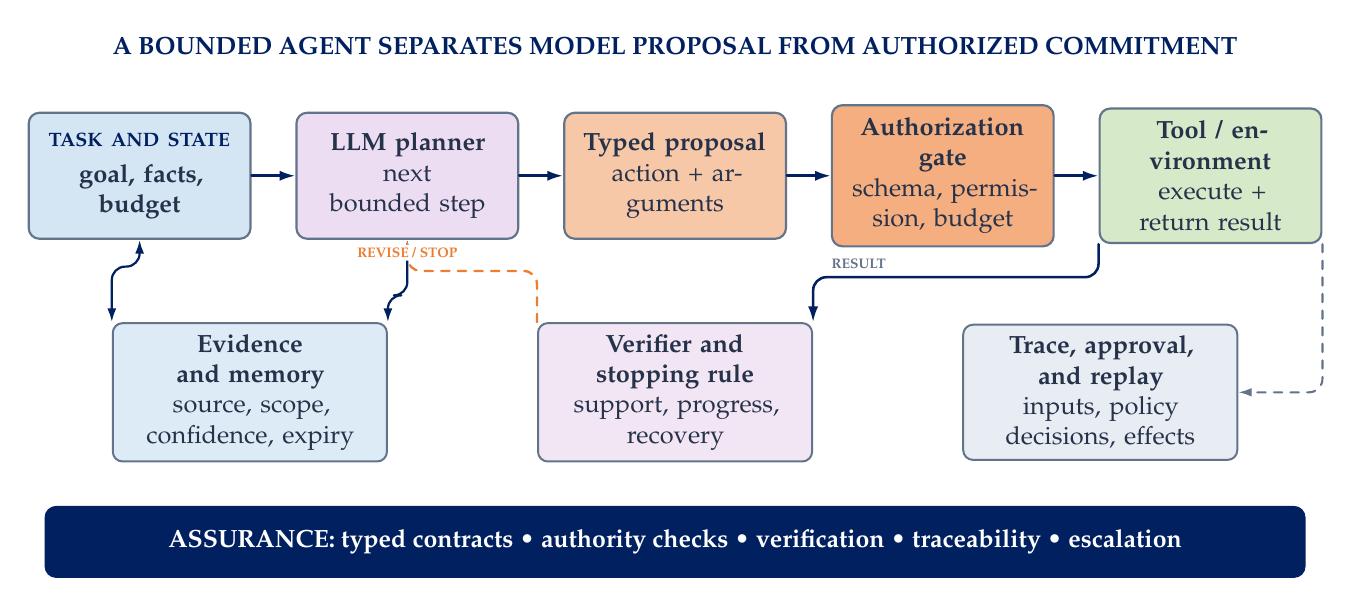
\begin{tikzpicture}[
  font=\small,
  line cap=round,
  line join=round,
  main/.style={
    rounded corners=1.35mm,
    draw=surveyLine,
    line width=0.78pt,
    align=center,
    text width=25mm,
    minimum height=16mm,
    inner sep=4.5pt,
    text=surveyInk
  },
  support/.style={
    rounded corners=1.25mm,
    draw=surveyLine,
    line width=0.72pt,
    align=center,
    text width=32mm,
    minimum height=12.5mm,
    inner sep=4pt,
    text=surveyInk,
    font=\small
  },
  arr/.style={
    -{Latex[length=2.0mm,width=1.3mm]},
    line width=0.92pt,
    draw=surveyNavy
  },
  data/.style={
    {Latex[length=1.75mm,width=1.15mm]}-{Latex[length=1.75mm,width=1.15mm]},
    line width=0.8pt,
    draw=surveyNavy
  },
  feedback/.style={
    -{Latex[length=1.9mm,width=1.2mm]},
    line width=0.85pt,
    dashed,
    draw=surveyOrange
  },
  trace/.style={
    -{Latex[length=1.7mm,width=1.1mm]},
    line width=0.75pt,
    dashed,
    draw=surveyLine
  }
]

\node[font=\small\bfseries,text=surveyNavy] at (0,1.65)
  {A BOUNDED AGENT SEPARATES MODEL PROPOSAL FROM AUTHORIZED COMMITMENT};

% The main path contains only the decisions that change authority or world state.
\node[main,fill=surveyBlue!43] (state) at (-6.80,0.00) {
  {\scriptsize\bfseries\color{surveyNavy}TASK AND STATE}\\[2pt]
  \textbf{goal, facts, budget}
};
\node[main,fill=surveyPurple!46] (planner) at (-3.40,0.00) {
  \textbf{LLM planner}\\
  next bounded step
};
\node[main,fill=surveyOrange!42] (proposal) at (0.00,0.00) {
  \textbf{Typed proposal}\\
  action + arguments
};
\node[main,fill=surveyOrange!62] (gate) at (3.40,0.00) {
  \textbf{Authorization gate}\\
  schema, permission, budget
};
\node[main,fill=surveyGreen!48] (environment) at (6.80,0.00) {
  \textbf{Tool / environment}\\
  execute + return result
};

\draw[arr] (state.east) -- (planner.west);
\draw[arr] (planner.east) -- (proposal.west);
\draw[arr] (proposal.east) -- (gate.west);
\draw[arr] (gate.east) -- (environment.west);

% Information and oversight sit below the main authority path so no arrow has
% to cut through a decision card.
\node[support,fill=surveyBlue!34] (memory) at (-5.40,-2.75) {
  \textbf{Evidence and memory}\\source, scope, confidence, expiry
};
\node[support,fill=surveyPurple!34] (verify) at (0.00,-2.75) {
  \textbf{Verifier and stopping rule}\\support, progress, recovery
};
\node[support,fill=surveyMuted] (tracebox) at (5.40,-2.75) {
  \textbf{Trace, approval, and replay}\\inputs, policy decisions, effects
};

% Orthogonal lanes keep evidence, feedback, and audit traffic visually distinct.
\draw[data,rounded corners=1.7mm]
  (state.south) -- ++(0,-0.34) -| (memory.north west);
\draw[data,rounded corners=1.7mm]
  (memory.north east) -- ++(0,0.34) -| (planner.south);
\draw[arr,rounded corners=1.7mm]
  (environment.south west) -- ++(0,-0.42) -|
  node[pos=0.42,above=1.5pt,font=\tiny\bfseries,fill=white,inner sep=1pt,text=surveyLine] {RESULT}
  (verify.north east);
\draw[feedback,rounded corners=1.7mm]
  (verify.north west) -- ++(0,0.65) -|
  node[pos=0.58,above=1.5pt,font=\tiny\bfseries,fill=white,inner sep=1pt,text=surveyOrange] {REVISE / STOP}
  (planner.south);
\draw[trace,rounded corners=1.7mm]
  (environment.south east) -- ++(0,-0.95) |- (tracebox.east);

\node[rounded corners=1.4mm,draw=surveyNavy,fill=surveyNavy,text=white,
  font=\small\bfseries,align=center,minimum width=16.00cm,minimum height=9mm]
  at (0,-4.65)
  {ASSURANCE: typed contracts \textbullet{} authority checks \textbullet{} verification \textbullet{} traceability \textbullet{} escalation};

\end{tikzpicture}

\caption{Reference architecture for bounded LLM-centered agents. The model plans and proposes a typed action, but an external gate authorizes the action against schemas, permissions, and budgets before any environment change. Evidence and memory inform the next decision; results are checked for support and progress; and approval plus trace paths preserve accountability.}
\label{fig:reference-architecture}
\end{figure}

\subsection{Control topologies}

Control topology is not merely the shape of an orchestration diagram; it determines which component selects the next transition, which state enables that transition, and how parallelism, recovery, and termination are represented. Workflow pattern research established that orchestration systems should be compared through observable control semantics, including sequence, choice, concurrency, synchronization, cancellation, and exception handling, rather than through vendor-specific syntax~\cite{vanderAalst2003workflowpatterns}. LLM-centered systems add three concerns to that classical lens: a proposed transition may be probabilistic, its supporting evidence may be incomplete or contested, and its execution may require separate authorization. We therefore compare each topology by five questions: where task state persists; who proposes the next step; how evidence, preconditions, permissions, and budgets are checked; how results and errors update subsequent decisions; and how the episode terminates or escalates. This lens separates architectural substance from labels: the same visible sequence can be implemented with very different state and authority boundaries, while a system with several named agents can still have one centralized controller.

\paragraph{Prompt loop.}
A prompt loop appends each observation to the transcript, asks the LLM for the next step, and repeats. ReAct demonstrates the value of this lightweight feedback structure~\cite{yao2023react}, but one transcript then serves as evidence, memory, plan, and program counter. AgentBench and WebArena show that model capability alone does not remove long-horizon control failures~\cite{liu2024agentbench,zhou2024webarena}. A production loop should externalize typed step, authorization, outcome, progress, and stopping records; otherwise replay reconstructs prose rather than state transitions. Prompt loops remain useful baselines, but incomplete production architectures.

\paragraph{Planner--executor.}
A planner--executor topology separates task decomposition from environment-specific action. Plan-and-Solve reduces missing-step errors in reasoning~\cite{wang2023planandsolve}, while Plan-and-Act extends the split to long-horizon web tasks~\cite{erdogan2025planandact}. The architectural value lies in the interface: the plan is versioned, prerequisites and permissions are checked at execution time, and typed outcomes can retain, repair, or invalidate later steps. This works when intent is stable but observations are volatile; it collapses into a prompt loop when the plan is only prose or the executor hides state and errors.

\paragraph{Graph or state machine orchestration.}
A graph or state machine represents process state and permitted transitions outside the model. StateFlow reports higher success and lower inference cost than ReAct on its InterCode SQL and ALFWorld evaluations~\cite{wu2024stateflow}. Nodes need typed inputs, effects, and success predicates; edges need guards and failure destinations; the runtime, not the LLM, commits transitions. This makes branching, intervention, replay, and recovery inspectable, but creates configuration cost and false assurance when guards still depend on stale prose or unchecked model judgment.

\paragraph{Event-driven architecture.}
An event-driven topology distributes control through messages. The actor model motivates modular message-driven behavior~\cite{hewitt1973actor}, while Lamport's partial ordering explains why causal identity and versioning matter~\cite{lamport1978timeclocks}. Events need typed identity, provenance, authorization context, and deduplication; delivery itself is not authority. Consumers must recheck state and permissions, tolerate duplicate delivery, and correlate results and retries. The topology supports asynchronous work and recovery, but introduces stale or reordered evidence, duplicate effects, races, and confused-deputy risk.

\paragraph{Hierarchical and multi-agent orchestration.}
A hierarchical or multi-agent topology delegates bounded work to managers, workers, or peers. MetaGPT demonstrates role and artifact coordination~\cite{hong2024metagpt}, and MultiAgentBench shows that topology and planning strategy affect milestone completion~\cite{zhu2025multiagentbench}. Delegation becomes architectural only through a task contract that limits evidence, tools, authority, budget, output, and success criteria. Workers return candidate results; a parent or arbiter admits them through provenance and conflict checks. This supports separable parallel work, but becomes costly when state is tightly coupled or the manager, shared context, or delegated authority becomes an unverified bottleneck.

\begin{table}[!htbp]
\centering
\caption{Common control topologies and their operational trade-offs.}
\label{tab:control-topologies}
\small
\surveytableformat
\begin{tabularx}{\textwidth}{L{2.6cm}Y Y Y}
\toprule
\rowcolor{surveyBlue!28}\textbf{Topology} & \textbf{Best suited to} & \textbf{Main advantage} & \textbf{Primary risk} \\
\midrule
Prompt loop & Low-risk prototypes and short tool tasks & Minimal implementation overhead & Implicit state, weak stopping, poor replay \\
Planner--executor & Multi-step tasks with well-defined tools & Separation of deliberation and actuation & Plans become stale; executor errors may be hidden \\
Graph/state machine & Auditable workflows with conditional branches & Explicit transitions, checkpoints, and recovery & Graph complexity and state version management \\
Event-driven & Long-running or asynchronous processes & Durability and scalable decoupling & Duplicate events, races, and partial failures \\
Hierarchical / multi-agent & Tasks benefiting from specialization or parallelism & Modular roles and permission isolation & Coordination overhead and correlated errors \\
\bottomrule
\end{tabularx}
\end{table}

\subsection{State and memory architectures}
\label{sec:memory}

In an agentic system, state and memory answer different operational questions. State is the authoritative, typed record required to determine and safely commit the next transition: the current step, evidence used, pending approvals, observed tool effects, budgets, and version. Memory is retained information that may be retrieved to inform later reasoning. The distinction appears from complementary directions in prior systems: StateFlow makes execution progress explicit through states and transitions~\cite{wu2024stateflow}, CoALA separates working, episodic, semantic, and procedural stores within an agent architecture~\cite{sumers2024coala}, and MemGPT manages movement between in-context and external memory~\cite{packer2024memgpt}. Once an agent can act on the world, however, this distinction becomes an integrity boundary. Retrieved memory should enter the current computation as a provenance-bearing candidate rather than silently overwrite authoritative task state; conversely, facts needed for recovery or authorization cannot survive only in a transcript, summary, or embedding. State therefore needs a schema, owner, version, invariants, and controlled updates, whereas memory needs relevance, provenance, freshness, retention, and access policies. Blurring the two produces systems that remember more language while preserving less operational truth.

\subsubsection{Functional memory layers}

A practical architecture separates at least five layers, not as progressively larger versions of the same store, but as representations that answer different control questions. The sequence below moves from information that must remain authoritative within the active run to information whose value emerges across tasks:
\begin{enumerate}
    \item \textbf{Execution state: What may occur next?} Authoritative progress, approvals, budgets, tool outcomes, and committed effects for continuation and recovery.
    \item \textbf{Working memory: What is active now?} Task-local hypotheses, constraints, candidates, and intermediate artifacts that remain provisional.
    \item \textbf{Episodic memory: What happened before?} Provenance-bearing trajectories and outcomes, as in Generative Agents~\cite{park2023generativeagents}.
    \item \textbf{Semantic memory: What is believed across episodes?} Versioned facts, preferences, concepts, and organizational knowledge with validity and source.
    \item \textbf{Procedural memory: How should the system act?} Reusable, revocable skills, plans, prompts, code, and lessons such as those extracted by ExpeL~\cite{zhao2024expel}.
\end{enumerate}
The layers therefore differ not only in update frequency and retention, but in authority. A retrieved episode or semantic record may become a candidate in working memory; it does not become an execution fact merely because it was retrieved. Conversely, a successful trajectory should not silently rewrite a shared skill. Information should cross these boundaries through explicit operations (retrieve, validate, admit, commit, consolidate, or discard) that preserve provenance and version history. This staged flow prevents a fluent summary or superficially similar memory from changing what the system is permitted to do.

\subsubsection{Representations and stores}

After deciding what role information plays, an architecture must choose how that information is represented. This is an operational decision: the representation determines which claims can be addressed exactly, which updates can be made atomically, whether provenance survives compaction, and whether recalled material can be distinguished from current authorization. No single form (raw transcript, summary, key--value record, embedding, relational table, knowledge graph, or executable artifact) supports all of these operations. Representative systems expose different parts of the trade-off. Generative Agents makes observation streams and synthesized reflections retrievable, supporting continuity in simulated social behavior but not supplying an authoritative transaction record~\cite{park2023generativeagents}. MemGPT manages movement between in-context and external memory, showing that location and access are themselves control decisions~\cite{packer2024memgpt}. MemoryBank makes retention, updating, and forgetting explicit, emphasizing the lifecycle of long-term conversational records~\cite{zhong2024memorybank}. Taken together, these designs argue for composite representation: typed records protect operational truth, provenance-bearing artifacts preserve evidence, and associative indices support recall without granting retrieved content authority by default.

\begin{itemize}
    \item \textbf{Transcripts} preserve chronology but mix observations, instructions, assertions, and tool returns; they are archives rather than canonical state.
    \item \textbf{Summaries} reduce context cost but can erase constraints and provenance, so they must link to source spans and transformation metadata.
    \item \textbf{Vector indexes} support semantic recall, but similarity does not establish truth, recency, permission, or applicability.
    \item \textbf{Structured records} support exact filters, invariants, atomic updates, and access control, making them the strongest fit for authoritative state.
    \item \textbf{Knowledge graphs} expose relations, time, and provenance, while leaving entity resolution and edge validity as explicit obligations.
    \item \textbf{Executable memory} stores code, plans, or skills, as in Voyager~\cite{wang2023voyager}; because retrieval can change behavior, it requires sandboxing, evaluation, versioning, and revocation.
\end{itemize}

The practical conclusion is a hybrid record, not a winning store. A task may keep authoritative status, budgets, and approvals in a typed transactional record; immutable source documents and tool receipts in an artifact store; embeddings or graph links as discovery indices; a derived summary for model context; and separately versioned procedures for reuse. Stable identifiers connect these views so that a retrieved passage can be traced to evidence and an action can be traced to the exact state and procedure that authorized it. The representation stack thus implements the paper's central boundary: associative memory proposes relevant material, while structured state determines what the system may commit.

\subsubsection{Memory operations as policy decisions}

A stored object becomes operational memory only through a lifecycle policy that decides when to create, link, retrieve, update, consolidate, or discard it, and which later decisions may consume it. Contemporary systems make different portions of that policy explicit. A-MEM generates attributes and links among records, so accumulated experience becomes a navigable relational structure~\cite{xu2025amem}; Mem0 selectively extracts and maintains long-term information from interactions~\cite{chhikara2025mem0}; and ExpeL transforms completed trajectories into reusable experiential lessons~\cite{zhao2024expel}. These are not interchangeable variants of one retrieval algorithm. They implement different typed transformations (event to linked record, interaction to retained fact, or trajectory to procedure) and grant the resulting object different authority. Reported gains on each system's native tasks therefore answer different questions. A meaningful comparison should identify the source object, transformation, retained provenance, intended consumer, and decision enabled, rather than collapse all results into a single memory leaderboard.

Every memory operation should be a typed, versioned event. Writes preserve source, scope, confidence, validity, and retention; reads return provenance, freshness, and conflicts; updates supersede rather than erase. AgeMem learns when to store, retrieve, update, and discard~\cite{yu2026agemem}, replacing fixed schedules with task-sensitive control. The same flexibility relocates risk into the learned policy, so schemas, authorization, versioning, and invalidation must remain independently enforced.

Personalized summarization provides an earlier example: feedback becomes an explicit preference model that changes later selection and synthesis~\cite{ghodratnama2023personalized,ghodratnama2024sumrecom}. In an acting system, that representation can alter tool choice, so an inferred preference may propose an update but cannot silently become durable authorization.


Memory benchmarks make the distinction empirical. MemBench tests factual and reflective recall~\cite{tan2025membench}, whereas Mem2ActBench tests whether remembered preferences and task state improve tool selection and argument grounding~\cite{shen2026mem2actbench}. Current systems are weaker at active use than retrieval-only results suggest. Evaluation must therefore follow write, retrieval, admission, decision, and effect; question answering establishes recall, not safe improvement to action.

\begin{table}[!htbp]
\centering
\caption{Representative memory designs. Results across rows are not directly comparable because the systems target different tasks and memory horizons.}
\label{tab:memory-evidence}
\small
\surveytableformat
\begin{tabularx}{\textwidth}{L{2.45cm}L{3.0cm}L{3.0cm}L{3.1cm}Y}
\toprule
\rowcolor{surveyBlue!28}\textbf{System} & \textbf{Memory object} & \textbf{Write or update policy} & \textbf{Evidence setting} & \textbf{Primary limitation} \\
\midrule
Generative Agents~\cite{park2023generativeagents} & Natural language observations, reflections, and plans & Stores observations; periodically synthesizes reflections & Interactive simulated social environment and human judgments & Simulation behavior does not establish factual or transactional reliability \\
MemGPT~\cite{packer2024memgpt} & In-context working memory plus external archival memory & Model-mediated movement between memory tiers & Long conversations and document analysis & Model-controlled paging can omit or retrieve the wrong state \\
Memory\-Bank\newline\cite{zhong2024memorybank} & Long-term conversational events and summaries & Updating and forgetting inspired by memory decay & Long-term dialogue and personality consistency & Conversation metrics do not test downstream tool action \\
ExpeL~\cite{zhao2024expel} & Reusable natural language lessons from trajectories & Reflects over successes and failures across episodes & Reasoning and interactive agent tasks & Extracted lessons can preserve evaluator errors \\
A-MEM~\cite{xu2025amem} & Linked notes with generated contextual attributes & Dynamically constructs and updates relationships & Knowledge and long-horizon agent tasks & Generated links and attributes require provenance validation \\
AgeMem~\cite{yu2026agemem} & Short- and long-term memory under a learned policy & Reinforcement-learned store, retrieve, update, and discard actions & Long-horizon agent memory benchmarks & Policy optimization broadens the attack and regression surface \\
\bottomrule
\end{tabularx}
\end{table}

\subsubsection{Memory failure modes}

Memory failures are not a miscellaneous collection of model mistakes; each violates a field or transition in the representation contract:
\begin{itemize}
    \item \textbf{Staleness (valid-time failure):} a once-correct item remains eligible after the world changes. Store valid-from and valid-to times, freshness requirements, and supersession links, and revalidate high-impact facts at use time.
    \item \textbf{Contamination (source type failure):} model-generated speculation is persisted as observation or evidence. Preserve typed source roles and require explicit promotion before an inference can enter semantic memory.
    \item \textbf{Scope leakage (access control failure):} information from one user, tenant, or task is retrieved in another. Experiments on Memory EXTRaction Attacks demonstrate that stored user--agent interactions create a practical privacy surface~\cite{wang2025memoryprivacy}; every record and query therefore needs subject, tenant, purpose, and permission labels.
    \item \textbf{Memory poisoning (integrity failure):} untrusted content crosses a write boundary and later steers decisions. A systematic study identifies multiple write channels and structural vulnerabilities and finds that more aggressive writing and retrieval can increase exploitability~\cite{dash2026memorypoisoning}. Separate trust domains, validate writes, and screen retrieved content before admission.
    \item \textbf{Over-retrieval (selection failure):} irrelevant or weakly matched memories crowd out current evidence. Bound retrieval budgets, filter by time and scope, diversify candidates, and require an admission decision rather than inserting all matches into context.
    \item \textbf{Under-retention (retention failure):} commitments, constraints, approvals, or unresolved obligations are discarded. Promote these objects to typed execution or semantic records with explicit retention rules instead of relying on lossy summaries.
    \item \textbf{Self-reinforcement (feedback failure):} repeated retrieval of an erroneous note increases its apparent credibility. Empirical work on experience-following reports both error propagation and misleading experience replay~\cite{xiong2026memorymanagement}; retrieval frequency must not substitute for independent evidence, and negative outcomes should reduce or revoke an item's eligibility.
\end{itemize}
Mitigation belongs at the failed boundary: provenance and type checks at write time; version, time, scope, and conflict filters at retrieval; authorization at admission; and reconciliation or revocation after truth changes. Cleanup alone is too late once a stale or poisoned item has influenced action. Every retained object needs an origin, every use an admissibility decision, and every invalidation a path to dependent state.

\subsection{Reasoning and planning}
\label{sec:planning}

Reasoning and planning are distinct transformations over system representations. Reasoning organizes evidence, constraints, hypotheses, and tests into intermediate claims; planning maps a goal and the accepted current state into an executable, versioned action structure. Classical planning makes the required semantics explicit through action preconditions and effects, as in STRIPS~\cite{fikes1971strips}, and through policies conditioned on uncertain observations, as in partially observable planning~\cite{kaelbling1998pomdp}. LLM scaffolds can propose these structures in natural language, but fluency does not remove the distinction: a rationale may omit evidence provenance, and a list of steps may be plan-shaped text without valid dependencies, permissions, or effects. A reliable architecture therefore separates a proposed rationale, a validated plan, the committed next action, and the observed result. Each transition should preserve typed inputs, ownership, success and failure conditions, and version history so that execution can reject, repair, or replan without treating the model's explanation as authority.

\subsubsection{Decomposition and explicit plans}

Decomposition becomes operational when subgoals are plan nodes rather than prose bullets. Least-to-most and Plan-and-Solve show benefits from staged reasoning~\cite{zhou2023leasttomost,wang2023planandsolve}; hierarchical task networks provide the stronger systems analogy of refinement under explicit constraints~\cite{erol1994htn}. A plan therefore needs versioned goals, dependencies, evidence, authority, expected effects, completion tests, and failure routes that a runtime can validate and schedule.

A plan is a versioned hypothesis, not a fixed commitment. Plan-and-Act separates construction from adaptive execution~\cite{erdogan2025planandact}; executor outcomes should therefore complete, block, fail, or invalidate nodes against observed effects. Contradictory evidence or unavailable authority creates a linked successor plan, while completed and irreversible effects remain part of history. Repair preserves valid work instead of restarting from a fresh prompt.

\subsubsection{Interleaved reasoning and acting}

Interleaving matters because pre-execution plans rest on untested predictions. ReAct shows the value of alternating decisions with observations~\cite{yao2023react}, but a free-form transcript blurs evidence, inference, authority, and effect. A production loop should persist the unresolved subgoal, evidence, assumptions, proposal, authorization, receipt, and state difference. The rationale may help the model; typed runtime fields make progress inspectable and resumable.

A useful loop is:
\begin{enumerate}
    \item select the next eligible unresolved subgoal from the current plan and state;
    \item assemble a scoped evidence bundle and record assumptions that remain unverified;
    \item propose an allowed action with typed arguments, expected effect, and success criterion;
    \item validate permissions, preconditions, schema, and budget, then execute with an idempotency or transaction identifier where possible;
    \item classify the observation, preserve the raw receipt, and derive a typed result and state difference;
    \item commit accepted updates, evaluate progress and termination conditions, and continue, repair, retry, escalate, or stop.
\end{enumerate}
Progress closes the loop by comparing accepted before and after state with completion predicates, not by counting tokens or steps. Fewer unresolved requirements, satisfied tests, accepted evidence, and confirmed effects establish movement. No-progress detection and resource limits bound repeated exploration, while termination records completion, partial completion, blockage, failure, or cancellation together with remaining obligations.

\subsubsection{Search and self-correction}

Search and self-correction improve a trajectory by creating and evaluating alternative representations, but the alternatives differ across methods. Tree-of-Thoughts materializes multiple intermediate states and uses an evaluator to select or prune branches~\cite{yao2023treeofthoughts}; Reflexion converts feedback from completed attempts into verbal episodic records that condition later trajectories~\cite{shinn2023reflexion}; and Self-Refine repeatedly transforms the current artifact through model-generated critique and revision~\cite{madaan2023selfrefine}. These are therefore not interchangeable instances of a single \emph{reflection} mechanism: one searches a state tree, one writes experience for a later episode, and one iterates over the same output. Their reported gains establish that additional structure and feedback can outperform a single greedy pass on their evaluated tasks, but not that self-generated evaluation is independent evidence. When the generator, critic, and selector share a blind spot, the loop may strengthen a coherent error rather than correct it.

A search controller should preserve candidate lineage, evidence, evaluator, result, rejection reason, and cost. Branching is justified by uncertainty and expected decision value; pruning should rely on executable tests, constraints, independent evidence, or human judgment. Termination depends on accepted solution criteria and the marginal value of another branch. Search earns its cost only when alternatives create better evidence for a bounded decision.

\subsubsection{Programmatic and symbolic planning}

Some reasoning and planning problems are better represented as programs, constraints, or symbolic operators than as free-form language. Program-Aided Language Models and Program-of-Thought prompting externalize arithmetic or symbolic computation into executable code~\cite{gao2023pal,chen2023pot}; STRIPS and PDDL make planning operators, preconditions, effects, objects, and goals explicit~\cite{fikes1971strips,mcdermott1998pddl}. These approaches strengthen different boundaries: code supplies deterministic execution for a specified computation, while a planning model supplies a search space with machine-checkable transition semantics. A hybrid agent can use an LLM to propose the formal representation and a parser, type checker, solver, or planner to reject malformed or unsatisfiable candidates. The translation itself remains a critical representation step, however: every variable, constraint, operator, and goal condition should be traceable to user intent, accepted evidence, or policy rather than introduced as an unsupported model assumption.

This pattern is strongest when generation is difficult but validity is cheap to check. A model may propose SQL, code, a schedule, or a symbolic plan; the environment parses, constrains, tests, or simulates it and returns a counterexample. Passing a validator does not prove that the specification captured user intent, so the artifact, specification, validator, result, and repair must remain linked. Executable checks strengthen evidence without eliminating provenance or high-impact review.

\subsection{Action selection and execution}
\label{sec:action}

Action selection is the boundary where a model proposal may become an external effect. Toolformer establishes proposal competence~\cite{schick2023toolformer}; $\tau$-bench shows why policy compliance and final task state matter beyond call selection~\cite{yao2024taubench}. The runtime must keep proposal, authorization, execution receipt, and independently observed effect distinct. A valid call is not necessarily permitted, and a success response is not proof of the intended state change. Schema-first interfaces, staged commitment, and explicit execution semantics constrain this transition.

\subsubsection{Schema-first interfaces}

A schema-first interface is an executable boundary, not a formatting hint. BFCL separates call conformance from long-horizon reliability and finds stronger performance on isolated calls than on memory and dynamic decision making~\cite{patil2025bfcl}. A tool contract should version the capability, inputs, outputs, scopes, side effects, preconditions, cost, idempotency, retry, and compensation. Descriptions help the model propose a call; the runtime binds and enforces the machine-readable contract.

Validation protects both directions. Before execution, the runtime canonicalizes arguments and checks resource identity, permission, state, preconditions, and budget. Afterward, it preserves the receipt, validates provenance and structure, and checks the claimed effect. InjecAgent's 1,054 cases show why returned content must remain untrusted evidence: its ReAct-prompted GPT-4 configuration followed attacks in 24\% of cases~\cite{zhan2024injecagent}. Schemas reject malformed structure; they do not establish permission, truth, or goal satisfaction.

\subsubsection{Read, propose, commit}

Read--propose--commit is a staged state transition protocol: it separates the evidence used to understand the environment, the candidate operation constructed from that evidence, and the authority to create an external effect. It is not equivalent to placing a human in every loop. Parasuraman, Sheridan, and Wickens distinguish automation of information acquisition, analysis, decision, and action, and argue that the level of automation should be chosen for each function~\cite{parasuraman2000levels}; Shneiderman likewise argues that high computer automation and high human control can coexist~\cite{shneiderman2020hcai}. For an agentic runtime, the architectural consequence is that automation and oversight can differ by stage, but every handoff must be represented explicitly:
\begin{enumerate}
    \item \textbf{read}: invoke only the observation capabilities authorized for the task and return a provenance-bearing record containing the source, query or resource, timestamp, state version, trust label, and raw receipt. A read does not change the target environment, although the runtime may append the observation to its audit and evidence stores;
    \item \textbf{propose}: materialize an immutable candidate containing the tool and schema version, canonical arguments, exact target resources, evidence references, expected state difference, uncertainty, cost, side effect and reversibility class, required permissions, and completion test. Dry runs, simulation, static checks, or diff generation attach validation evidence to this proposal rather than silently modifying it;
    \item \textbf{commit}: have a policy gate or authorized person evaluate that exact proposal and persist the decision with principal, policy version, granted scopes, constraints, expiry, and proposal identifier. The executor rejects a stale or altered proposal, applies an idempotency or transaction identifier, and returns both an execution receipt and a separately validated effect record.
\end{enumerate}
Approval is a versioned capability grant, not conversational assent. A change to arguments, target state, schema, evidence, or predicted effect invalidates the grant. Review should expose the concrete diff, target, uncertainty, and reversibility; graduated authority can automate inspection while reserving consequential commits. Reads still carry privacy and cost, and approval does not prove correctness, so least privilege and post-effect validation remain necessary.

\subsubsection{Execution semantics}

Authorization does not remove execution ambiguity: after a timeout or broken connection, the effect may have failed, succeeded, or partially applied. The runtime must distinguish the logical operation, each attempt, and observed world state. Its lifecycle separates authorization, dispatch, acknowledgement, and effect verification, together with denial, ambiguity, partial application, and compensation. A plan node is satisfied by verified state change, not a response string.

Recovery follows the result class. Invalid or denied proposals wait for changed input or authority; transient failures permit bounded backoff; unknown effects require status reconciliation before a side-effecting retry. Attempts remain linked to one logical operation. For non-atomic workflows, sagas provide explicit compensation~\cite{garciamolina1987sagas}; compensation is itself an authorized, fallible action rather than erasure of history.

Tool returns should be normalized into typed success, partial, denied, unavailable, ambiguous, or terminal outcomes while preserving the receipt. AppWorld's state-based tests across 750 tasks and 457 APIs show why effect evidence matters; its strongest reported GPT-4o configuration reached 48.8\% on normal and 30.2\% on challenge tasks~\cite{trivedi2024appworld}. Invocation and fluent explanation are weak proxies for success, so continuation or recovery must follow the validated state difference.

\subsubsection{Tool selection at scale}

At catalog scale, tool selection is constrained retrieval over a changing capability space rather than classification over every description in the prompt. ToolLLM makes the retrieval problem explicit: ToolBench collected 16,464 real-world APIs across 49 categories, and ToolLLaMA uses a neural API retriever to recommend a tractable candidate set~\cite{qin2024toolllm}. BFCL exposes a complementary limit: models that perform strongly on single-turn calls still face open challenges in stateful, multi-step decision making, and the benchmark explicitly evaluates abstention~\cite{patil2025bfcl}. Together, these results separate three questions that are often collapsed: whether the catalog contains a useful capability, whether retrieval surfaces it, and whether the current task state and authority permit its use. A semantically relevant tool may still be unavailable, obsolete, too costly, insufficiently trusted, or outside the actor's scope.

The capability registry should be authoritative and versioned rather than appended to a prompt. Entries expose schema, authority, side effects, health, cost, version, and validation status. Deterministic filters first remove unauthorized or incompatible tools; retrieval ranks the admissible remainder; the model selects or abstains within that bounded set. Permissions, health, and schemas are revalidated at dispatch.

Hierarchical routing reduces context cost but can hide the only valid tool, so candidate recall must be measured separately from call accuracy. Fallbacks require compatible semantics, permissions, side effects, and outputs. Evaluation should distinguish catalog coverage, retrieval, selection, authorization, execution, effect correctness, collateral change, latency, and cost.

\subsection{Learning and adaptation}
\label{sec:learning}

Learning and adaptation is the boundary at which runtime evidence becomes a persistent change to future behavior. A completed trajectory contains observations, decisions, actions, receipts, effects, feedback, and cost, but a successful outcome does not by itself identify which element caused the success or whether the behavior should generalize. The relevant literature changes different substrates: ExpeL extracts reusable natural language lessons from experience~\cite{zhao2024expel}; Voyager adds executable skills to a growing library~\cite{wang2023voyager}; and SOAR optimizes an agentic tool use policy from observed behavior~\cite{li2026soar}. The self-improvement taxonomy further distinguishes updates to foundation model parameters from updates to the surrounding scaffold, including prompts, memory, tools, and control logic~\cite{ren2026selfimprovingagents}. These mechanisms are not interchangeable. A textual lesson, executable procedure, routing statistic, memory item, and weight update have different scope, authority, failure modes, evaluation costs, and rollback semantics. The architectural question is therefore not simply whether an agent learns, but which representation changes, from what accepted evidence, for whose future tasks, and under whose authority.

A production learning pipeline links immutable trajectories to candidate lessons, skills, prompts, memory policies, routers, or model updates. Each candidate needs scope, source evidence, expected benefit, risks, evaluation, approval, and rollback. Temporary within-episode adaptation may remain working state; shared changes require comparative testing against a frozen baseline and monitored promotion. This staging limits feedback contamination, reward hacking, and durable regressions.

\subsubsection{Learning from trajectories}

A trajectory becomes supervision only when its state transitions, evidence, proposals, authority, receipts, effects, costs, and evaluator remain attributable. Behavioral cloning inherits demonstration bias; preference optimization depends on shown comparisons and judges; reinforcement learning depends on delayed and potentially misspecified reward. Successful, failed, denied, corrected, and compensated episodes therefore provide different evidence and should not be collapsed into one undifferentiated transcript.

Recent methods expand the learned object beyond the final action. SOAR explicitly treats environment observations as supervision rather than assigning learning signal only from outcome rewards; across three domains and 14 benchmarks, it reports gains of up to 7.0\% on general reasoning and 16.9\% on deep research tasks, together with fewer erroneous or inefficient tool uses~\cite{li2026soar}. SUPO jointly optimizes tool behavior and the summaries used to compress long interaction histories, making context management part of the policy rather than a fixed preprocessing rule~\cite{lu2026supo}. AgeMem exposes store, retrieve, update, summarize, and discard operations as actions and trains unified short- and long-term memory management across five long-horizon benchmarks~\cite{yu2026agemem}. These methods target different representations (action consequences, compressed context, and memory operations), so their gains should not be summarized as generic evidence that additional trajectory learning is uniformly better. They instead show that the placement and granularity of credit determine which component learns from the same episode.

A trajectory-to-training pipeline must preserve provenance, evaluator reliability, environment and tool versions, sampling, objective, data splits, and the produced artifact. Held-out evaluation should compare with a frozen baseline on outcome quality, violations, collateral effects, calibration, efficiency, and regressions. Only an artifact that passes explicit promotion criteria should alter deployed policy. Learning is a controlled transformation of execution evidence, not replay of whatever received a favorable score.

\subsubsection{Online adaptation and self-improvement}

Online adaptation shortens the interval between feedback and behavioral change, but the literature uses the label for materially different persistence mechanisms. Reflexion converts task feedback into verbal records retained in an episodic memory buffer for later trials~\cite{shinn2023reflexion}; ExpeL aggregates experiences from training tasks into natural language insights and retrieves both insights and prior episodes at inference~\cite{zhao2024expel}; Voyager refines executable programs from environment feedback and commits successful programs to a reusable skill library~\cite{wang2023voyager}. In its Minecraft evaluation, Voyager reports 3.3 times more unique items, 2.3 times longer travel, and technology tree milestones reached up to 15.3 times faster than prior systems, while also reusing its skill library in a new world. These results support explicit scaffold adaptation in that environment, not a general claim that self-written memories or code are safe to share or deploy. The broader self-improvement taxonomy is therefore important: foundation model updates, prompt changes, memory writes, tool or skill updates, and control logic revisions modify different representations and require different evidence~\cite{ren2026selfimprovingagents}.

Adaptation should be classified by blast radius: episode-local state, subject- or task-scoped memory, shared scaffolds, and model parameters. Promotion thresholds grow with persistence, privilege, and audience. A temporary hint may need local checks; a shared executable skill needs provenance, sandbox and held-out tests, approval, staged rollout, monitoring, and rollback.

Generation, evaluation, and promotion authority must remain separate. Feedback can be noisy, manipulated, or privacy-sensitive, and persistent stores enlarge integrity and disclosure risks~\cite{dash2026memorypoisoning,wang2025memoryprivacy}. Candidate changes should be quarantined and tested against independent effects, invariants, held-out tasks, or accountable review. Bounded self-improvement requires a precise answer to what changed, why, where it applies, and how it can be revoked.

\subsection{Hierarchical agency}
\label{sec:hierarchy}

Hierarchical agency is a representation of nested responsibility: it determines which controller owns the root objective and authoritative state, which subgoals and capabilities may be delegated, and which evidence permits a child result to change the parent plan. Classical abstractions make these obligations concrete. An option is a temporally extended action defined by an initiation set, an internal policy, and a termination condition~\cite{sutton1999options}; hierarchical task network planning refines abstract tasks into constrained networks of subtasks~\cite{erol1994htn}. Plan-and-Act instantiates the same separation in an LLM agent through a structured high-level planner and an environment-specific executor, reporting a 54\% success rate on WebArena-Lite~\cite{erdogan2025planandact}. These results support hierarchy as a way to divide long-horizon control, but they do not justify multiplying conversational roles. Whether implemented with one model at several control levels or with several agents, the hierarchy resides in state ownership, admissible transitions, and completion authority.

The task tree is therefore a persistent control structure rather than a transcript outline. A parent retains the root task identifier, objective, global plan version, authoritative state, policy and budget envelope, and final completion authority. A child receives a versioned snapshot for a bounded subtask and owns only the local state needed to execute it. Manager--worker delegation, planner--executor separation, reusable skill libraries, and task graphs are useful only when their boundaries align with different context, evidence, tools, permissions, or verification duties. Privilege separation follows naturally: research and planning children may retrieve evidence and propose actions, while a narrowly scoped executor alone holds commit capabilities. A delegation should expire or be revoked when its parent plan, input evidence, permission, or target state version changes.

A delegation contract should specify:
\begin{itemize}
    \item \textbf{identity and lineage:} stable task, parent, plan version, dependency, and assignee identifiers;
    \item \textbf{objective and entry conditions:} the bounded subgoal, constraints, preconditions, and assumptions;
    \item \textbf{input state and evidence:} referenced artifacts, provenance, freshness, and the state version from which the child starts;
    \item \textbf{capability envelope:} allowed tools, data, permissions, action classes, time, tokens, and monetary budget;
    \item \textbf{return schema:} required artifacts, claims with evidence references, expected effects, and proposed state delta;
    \item \textbf{exit conditions:} machine-checkable success tests, retry limits, failure classes, and escalation route; and
    \item \textbf{delegation policy:} whether further delegation is allowed, its depth and authority limits, and expiry or cancellation conditions.
\end{itemize}

Return is a second typed boundary. A child should report a status, produced artifacts and claims, supporting evidence, action receipts and verified effects, its proposed state delta, unresolved assumptions, consumed budget, and a recommended parent transition. The parent then checks the contract, evidence, permissions, completion predicate, and referenced state versions before admitting the result. It may accept, reject, request repair, escalate, or invalidate dependent nodes; the child should not overwrite authoritative root state directly. This admission step prevents a fluent completion message from being mistaken for completion and localizes rework when a branch fails.

The architectural trade-off is between global consistency and local autonomy. Centralized parents simplify prioritization, conflict resolution, and budget control but can become decision and context bottlenecks. More autonomous children permit specialization and parallel progress, but increase stale state, duplicated work, reconciliation, and authority risks. Hierarchy is therefore justified when subproblems can be separated along state, data, tool, or permission boundaries and their outputs can be tested before merge. It should be evaluated through milestone completion, accepted handoffs, rework and conflict rates, escalation frequency, latency and cost, and privilege violations, not by the number of agents, roles, or exchanged messages.

\subsection{Multi-agent coordination}
\label{sec:multiagent}

Multi-agent coordination distributes work, evidence, and control authority. AutoGen emphasizes programmable conversations~\cite{wu2023autogen}, CAMEL role-conditioned interaction~\cite{li2023camel}, and MetaGPT specialized roles and artifacts~\cite{hong2024metagpt}. The architectural question is what information and authority are genuinely separated and how contributions are reconciled. Membership, state ownership, messages, permissions, conflict resolution, termination, and accountability, not the number of model calls, define the system.

\subsubsection{Coordination topologies}

Topology determines which participants can observe state, assign work, communicate evidence, resolve conflicts, and authorize a shared transition. Four patterns recur:
\begin{itemize}
    \item \textbf{centralized}: a manager owns the root plan and authoritative ledger, issues versioned task contracts, and admits validated results;
    \item \textbf{peer-to-peer}: participants own local state and exchange typed proposals, evidence, acknowledgments, and conflict notices without a permanent central integrator;
    \item \textbf{blackboard}: participants coordinate through a shared structured workspace whose records expose partial solutions and unresolved needs~\cite{nii1986blackboard};
    \item \textbf{market or contract}: a task is announced with constraints and an evaluation rule, candidates bid their capability, cost, or expected utility, and assignment becomes an explicit contract~\cite{smith1980contractnet}.
\end{itemize}

These patterns change the failure surface rather than defining a universal ranking. Centralization simplifies global prioritization, least privilege enforcement, and final accountability, but concentrates context, queueing, and recovery in one manager. Peer-to-peer structures remove that chokepoint and can support local adaptation, yet require explicit discovery, synchronization, duplicate work detection, and distributed conflict resolution. A blackboard decouples producers from consumers and preserves visible intermediate state, but only if writes are atomic, versioned, attributable, access-controlled, and invalidated when upstream evidence changes. Contract-based allocation makes selection criteria observable and can allocate heterogeneous capabilities dynamically, while adding bidding latency and the risk that self-reported capability or cost is poorly calibrated.

Contemporary evidence reinforces this conditional view. MultiAgentBench compares star, chain, tree, and graph protocols across interactive collaboration and competition scenarios; it reports that the graph protocol performed best in its research scenario and that cognitive planning increased milestone achievement by three percentage points~\cite{zhu2025multiagentbench}. This is evidence that topology and planning policy affect progress, not that graph communication is globally superior. A sound design should choose the narrowest topology that matches the dependency structure: centralized control when state is tightly coupled or authority must remain singular; peer or graph communication when dependencies are local and dynamic; a blackboard when several specialists must contribute asynchronously to a common artifact; and contracting when task allocation itself is uncertain. Hybrids are often appropriate: for example, a central authority may control commits while workers exchange evidence through a shared blackboard and receive work through explicit contracts.

The topology should be persisted as configuration rather than implied by prompts. It defines membership, capability, permission, state ownership, communication, allocation, merge, escalation, budget, termination, and reconfiguration authority. Runtime measures of stale reads, duplicate work, conflicts, latency, privilege violations, and accepted progress distinguish useful distribution from multiplying the same reasoning path.

\subsubsection{Communication and aggregation}

Communication is where local observations and proposals become candidates for shared state. FIPA-style performatives distinguish requests, reports, proposals, agreements, and refusals from their payloads~\cite{fipa2002communicative}; LLM systems need the same separation even when content remains natural language. A typed message envelope binds sender, recipient, task and state versions, evidence, requested transition, authority, uncertainty, causality, expiry, and acknowledgment so operational meaning is not inferred from style.

Delivery is not acceptance. The recipient should validate the sender's identity and delegated authority, parse the declared schema, resolve evidence references, compare state and plan versions, and check freshness, policy, and budget before the message changes a task or triggers an action. It should persist whether the message was received, rejected, admitted, superseded, or awaiting repair, together with the validator and reason. This protocol state supports replay, deduplication, timeout handling, cancellation, and accountability; it also prevents quoted instructions, stale plans, and unsupported claims inside one agent's output from silently controlling another. Natural language explanation can remain attached for human and model interpretation, but the executable consequence must be selected from an explicit transition set.

Aggregation is a separate admission problem: several contributions must be transformed into one decision without erasing their provenance or dissent. Objective validation should dominate when answers or effects can be tested. Evidence-aware selection can score source quality, coverage, recency, and contradiction; majority vote is defensible only when candidate errors are sufficiently independent; confidence weighting requires calibration on the relevant task distribution; and debate followed by a judge adds value only if interaction exposes information that independent sampling would miss. Du et al. report factuality and reasoning gains from iterative multi-agent debate in their studied settings~\cite{du2024multiagentdebate}. Smit et al., however, find that debate protocols do not reliably outperform self-consistency or ensembles of independent reasoning paths without careful tuning, while showing that agreement intensity can materially change results~\cite{smit2024mad}. Explanation-mediated weak-to-strong supervision provides another structured exchange of claims, critiques, and supervisory signals~\cite{zakershahrak2024explanation}. Together, these results argue for treating communication and aggregation as evaluated algorithms, not assuming that discussion produces verification.

The admitted decision should preserve candidates, evidence, eligibility, verifier results, aggregation rule, conflicts, selected result or abstention, and accountable authority. Agreement is weak evidence when agents share models, prompts, corpora, or context. Meaningful diversity must come from different evidence, tools, permissions, models, or verification functions; correlated failure should remain explicit.

Evaluation should compare the protocol with one agent, independent sampling, and deterministic verification. Message validity, duplication, disagreement, judge calibration, communication cost, and accepted progress expose coordination value. MultiAgentBench confirms that topology and planning alter milestone progress~\cite{zhu2025multiagentbench}; additional agents are justified only when evidence, specialization, or verification pays for reconciliation.

\subsubsection{Multi-agent failure modes}

Multi-agent failures are usually failures of represented coordination before they are failures of model count. Cemri et al. construct the Multi-Agent System Failure Taxonomy from 150 expert-annotated execution traces and scale the accompanying dataset to more than 1,600 traces across seven frameworks; its 14 failure modes fall into system design, inter-agent-misalignment, and task verification categories~\cite{cemri2025mast}. This evidence is important because it localizes failure in the protocol that connects agents, rather than treating an unsuccessful final answer as an undifferentiated model error. The three categories correspond to missing or violated representation contracts:
\begin{itemize}
    \item \textbf{specification and system design:} task or role constraints are not encoded and checked; steps repeat because completion is not persisted; relevant history disappears; or no controller owns a termination condition;
    \item \textbf{inter-agent misalignment:} agents fail to request clarification, drift from the assigned task, withhold or ignore relevant evidence, reset the conversation, or describe reasoning that does not match the action taken; and
    \item \textbf{verification and termination:} the system stops before postconditions hold, performs no or incomplete verification, or admits an incorrect check as proof of completion.
\end{itemize}

The categories interact: an underspecified contract creates divergent interpretations, untyped messages hide them, shared state admits incompatible claims, and weak completion tests convert agreement into success. Duplicate work, stale state, and premature consensus are propagation paths. MultiAgentBench exposes repetition and inefficient collaboration~\cite{zhu2025multiagentbench}; containment therefore requires lineage from the first violated contract to dependent claims, plans, actions, and effects.

A typed incident should identify the failed contract, task and plan versions, evidence, affected artifacts and effects, retryability, containment owner, and disposition. Detection moves work through blocked, quarantined, repairing, compensating, escalated, or failed states and invalidates dependent state. Specification, alignment, and verification failures require different controls; none is repaired by another unsupported completion claim.

Recovery is part of coordination. Retries preserve operation and failure identity and avoid duplicate effects; partial success may require compensation or a successor plan. Failed workers return usable artifacts and unresolved obligations so only unfinished work is reassigned. Failed managers require externally persisted root state and takeover rules. Human escalation should carry the incident and a precise decision request, not the entire transcript.

Multi-agent value must be measured against coordination burden. Compare failure propagation, duplicate execution, stale handoffs, conflicts, recovery, privilege violations, messages, latency, and cost with a single agent and independent samples. If distribution does not produce measurable gains from parallelism, complementary evidence, specialization, or independent verification, one agent with explicit modules is usually more reliable.

\subsection{Interoperability: tools, context, and agent-to-agent communication}
\label{sec:protocols}

Interoperability externalizes the representation contract across process, vendor, and organizational trust boundaries. It determines how a remote capability is discovered, how inputs and outputs are serialized, how long-running work is tracked, and how one system relates a returned artifact to its own task state. Syntactic compatibility is necessary but insufficient: a valid protocol message does not establish that the sender is trustworthy, the capability is appropriate, the request is authorized, the response is true, or an intended external effect occurred. Two protocol families address complementary parts of this problem.

\paragraph{Model Context Protocol (MCP).}
MCP standardizes how an AI host connects through clients to servers that expose tools, resources, and prompts. The specification defines a stateful, capability-negotiated protocol over JSON-RPC and standard transports~\cite{mcp2025spec}. Its durable architectural contribution is a common description and invocation surface: a tool can declare an input schema and optional output schema; a resource has a URI and metadata; requests, responses, notifications, progress, errors, and cancellation can be correlated. The declaration is still a capability claim made by a server. A host should persist the server identity and protocol version, negotiated capability snapshot, tool or resource identifier and schema version, validated arguments, authorization context, request and result identifiers, returned content and structured output, errors, timing, and cost. Returned text or data becomes an observation with provenance, not an instruction or verified effect.

MCP authorization mechanisms can authenticate parties, discover authorization servers, bind tokens to intended resources, and constrain scopes, but authentication and token validity do not answer whether a particular agent should perform a particular action in the current task. The application must still map the authenticated principal and granted scopes to a local capability policy, obtain any required user approval, recheck current state and budget, and validate the observed effect after invocation. This preserves the read--propose--authorize--execute--verify sequence even when the connector is standardized.

\paragraph{Agent2Agent (A2A).}
A2A standardizes interaction between independent agents. An Agent Card advertises identity, endpoint, skills, interfaces, and security requirements; exchanges use messages for immediate communication and tasks for stateful work that can produce status updates and artifacts~\cite{a2a2026spec}. This makes remote delegation more explicit than forwarding a chat prompt, but an advertised skill is not evidence that the agent is competent, available, authorized, or safe for the requested data. The delegating system should therefore translate its local subtask contract into an A2A task linked to the parent task, evidence snapshot, permission and data use envelope, expected artifact schema, budget, deadline, and completion test. It should persist the remote Agent Card and version used, endpoint and authenticated principal, task and context identifiers, messages, task state transitions, artifacts, cancellation or input requests, and terminal status.

The parent retains admission and completion authority. A remote \emph{completed} state means that the remote protocol lifecycle ended successfully; it does not prove that local postconditions hold. Likewise, an authentication or authorization-required state does not itself grant permission for an operation. Returned artifacts must pass provenance, schema, policy, freshness, and task-specific verification before they update the parent plan or trigger a local action. This distinction permits agents operated by different organizations to collaborate without silently merging their trust domains.

\begin{table}[H]
\centering
\caption{Complementary representation boundaries of MCP and A2A. Both require application-owned authorization, verification, and trace continuity.}
\label{tab:protocols}
\small
\surveytableformat
\begin{tabularx}{\textwidth}{L{2cm}Y Y}
\toprule
 & \textbf{MCP} & \textbf{A2A} \\
\midrule
Primary boundary & Host application to tools and context providers & Delegating agent to an independent remote agent \\
Advertised surface & Tools, resources, prompts, schemas, capabilities & Agent Card, skills, interfaces, security schemes \\
Persistent unit & Session plus correlated request, result, progress, or error & Message or stateful task with status and context \\
Returned record & Content, structured output, resource link, or error & Message, task status, artifact, or terminal outcome \\
Typical use & Connect an agent to files, databases, APIs, or services & Delegate bounded work to a specialized agent \\
Not guaranteed & Local authorization, output truth, or verified effect & Competence, shared policy, or local task completion \\
\bottomrule
\end{tabularx}
\end{table}

The protocols can be composed without conflating them. A parent may create an A2A task for a remote specialist, while that specialist uses MCP clients to obtain evidence or invoke tools. The end-to-end trace should preserve one lineage from the root request and evidence snapshot, through the delegation contract and remote task, to every MCP invocation and receipt, produced artifact, independently observed effect, and parent admission decision. Correlation identifiers alone are insufficient if each hop discards the state version, authority, or evidence that justified it; the application needs a cross-protocol trace record that binds those fields explicitly.

Protocol adoption also expands the supply chain. A registry, server, adapter, or remote agent may be compromised, stale, misconfigured, or simply unreliable. Clients should authenticate endpoints, negotiate and pin compatible protocol and schema versions, record the capability snapshot used for each decision, minimize scopes and disclosed data, enforce time and cost bounds, validate structured inputs and outputs, make side-effecting retries idempotent, support cancellation and revocation, and quarantine untrusted returned content. Capability discovery is not authorization, authentication is not trust, delivery is not acceptance, and protocol completion is not effect verification.

Because these specifications define interfaces rather than empirical reliability guarantees, evaluation should test both conformance and application behavior. A compatibility matrix should exercise supported transports, protocol versions, capabilities, schemas, authentication modes, streaming, cancellation, and failure responses across independent implementations. End-to-end measures should include discovery-to-invocation success, stale capability and version negotiation failures, authorization denials and scope escalation, schema-valid output, trace completeness across hops, cancellation and retry correctness, task and effect success, latency, and cost. Security tests should include malicious capability descriptions, prompt injection in resources or artifacts, forged or confused identities, token audience errors, oversized responses, and unavailable peers. Comparisons with a native connector or local agent should report whether standardization reduces integration work without weakening the bounded transition controls required by the application.

\subsection{Framework landscape}
\label{sec:frameworks}

An agent framework is not the architecture itself; it is a runtime and set of defaults for representing some parts of that architecture. It may externalize graph state while leaving authorization to application code, make handoffs explicit while keeping task completion conversational, or provide tracing without durable recovery. Feature checklists age quickly as APIs, product names, and maturity levels change. A more durable comparison asks which evidence, state, control, and authority boundaries a framework makes inspectable and enforceable, and which remain implicit or must be supplied by the application.

\begin{table}[H]
\centering
\caption{Representative framework categories classified by their externalized representations. Entries are illustrative; documented primitives are not reliability guarantees.}
\label{tab:framework-landscape}
\small
\surveytableformat
\begin{tabularx}{\textwidth}{L{2.7cm}L{2.7cm}Y Y}
\toprule
\rowcolor{surveyBlue!28}\textbf{Category} & \textbf{Representative systems} & \textbf{Externalized representation} & \textbf{Architectural evidence to verify} \\
\midrule
Graph/workflow orchestration & LangGraph; Semantic Kernel & Nodes, typed state, guarded edges, checkpoints, interrupts & Persistence and resume semantics; approval scope; idempotent side effects; failure edges \\
Agent conversation & AutoGen; CrewAI & Agents, roles, messages, tasks, handoffs & Ownership and message schemas; shared state merge; authority; termination and admission \\
Data/RAG-centered agents & LlamaIndex; Haystack & Documents, indexes, retrievers, typed pipelines, tools & Provenance, access and refresh policy, retrieval evaluation, action state integration \\
Native agent runtimes & OpenAI Agents SDK; Google ADK & Agents, tools, handoffs, sessions, guardrails, traces & Model portability; durable recovery; policy boundary; trace and evaluation export \\
Interoperability protocols & MCP; A2A & Capability schemas, Agent Cards, tasks, messages, artifacts & Authentication, trust and admission boundaries, version negotiation, conformance \\
Research prototypes & AutoGPT; BabyAGI and related loops & Open-ended plan, task list, memory, and iteration loop & Historical influence; state, authorization, verification, and recovery that must be added \\
\bottomrule
\end{tabularx}
\end{table}

Primary documentation illustrates the variation in what is made explicit. LangGraph describes checkpointed graph state and resumable interrupts~\cite{langgraph2026persistence}; Semantic Kernel exposes multiple agent orchestration patterns while marking important orchestration features as experimental~\cite{microsoft2025semanticagents}; and Haystack defines schema-based shared agent state with typed component inputs and outputs~\cite{deepset2026haystackstate}. AutoGen emphasizes programmable agent conversation~\cite{wu2023autogen}; the OpenAI Agents SDK exposes agents, tools, handoffs, guardrails, sessions, and tracing~\cite{openai2025agentssdk}; and Google ADK documents agents, tools, sessions, state, callbacks, evaluation, and deployment abstractions~\cite{google2026adkdocs}. These sources establish interface capabilities, not comparative production reliability. MAST's observation of recurring coordination failures across seven multi-agent frameworks reinforces that adopting a framework does not remove the need for explicit contracts, verification, and recovery~\cite{cemri2025mast}.

Framework selection should therefore begin with a representation matrix, not a catalog of integrations. For every required record (the evidence bundle, task and plan node, memory item, tool schema, action proposal, approval, execution receipt, verified effect, incident, and trace), the team should state whether the framework owns it, merely transports it, or leaves it to application code. The same matrix should locate who may create, mutate, approve, invalidate, and inspect each record. A versioned framework selection record can then capture candidate and dependency versions, requirements, gaps, adapters, security and data boundaries, operating limits, the evaluation baseline, and migration and rollback conditions. This turns framework choice from a one-time preference into an auditable architectural decision.

Portability depends on preserving the application's semantic state outside framework-specific transcripts and identifiers. Adapters should map canonical application records into framework nodes, sessions, handoffs, or events, and map framework results back into typed outcomes. Prompts, tool schemas, policies, evaluators, and traces should be versioned independently where practical. An upgrade is safe only when it cannot silently change the meaning of stored state, completion, authorization, or recovery.

Finally, a proof-of-fit should execute one representative long-horizon workflow with fixed models, tools, evidence, and budgets. It should test restart from checkpoint, approval edits and invalidation, duplicate delivery, malformed tool output, stale evidence, timeout, cancellation, partial side effects, worker failure, and trace export. Report task success and verified effect success separately, together with recovery and replay success, policy violations, trace completeness, latency and cost, required custom code, and behavior under injected faults. The preferred framework is the one that provides the smallest trustworthy extension surface for the system's actual obligations, not the one with the longest feature list.

\subsection{Reference design principles}

The preceding architectures can be synthesized as a chain-of-custody problem. Evidence is not yet operational state; state is not authorization; a successful API response is not a verified effect; and a plausible final answer is not proof that the intervening process was acceptable. Modern agentic systems become governable when each conversion is represented by a typed, persistent record and admitted through an explicit transition. The following principles are therefore coupled design obligations rather than an independent feature checklist.

\begin{enumerate}
    \item \textbf{Minimize adaptive control.} A model should decide only where the system genuinely needs semantic interpretation, uncertain judgment, or open-ended generation. Routing rules, eligibility constraints, budgets, authorization checks, and terminal conditions should remain deterministic whenever they can be specified. StateFlow's state-driven workflows illustrate how explicit states can organize model calls~\cite{wu2024stateflow}, while long-horizon benchmarks such as $\tau$-bench and AppWorld show that fluent tool use does not by itself produce consistent rule following or correct environment state~\cite{yao2024taubench,trivedi2024appworld}. The model should therefore emit a proposal with a reason code and supporting evidence; a deterministic controller should decide whether that proposal is an admissible transition.

    \item \textbf{Make state explicit.} Every consequential decision should read from and write to a declared state model rather than depend on facts recoverable only from a transcript. At minimum, the architecture should externalize evidence bundles, task and plan nodes, memory items, action proposals, approvals, execution receipts, verified effects, incidents, budgets, and termination status. Each record needs an identifier, type, schema version, provenance, owner, timestamps, and lifecycle state. Cognitive agent architectures motivate the separation of working, episodic, semantic, and procedural state~\cite{sumers2024coala}; LangGraph's checkpoints and Haystack's schema-based agent state provide current implementation examples~\cite{langgraph2026persistence,deepset2026haystackstate}. These primitives are useful only when the application also defines merge, invalidation, retention, and authority semantics.

    \item \textbf{Treat tools as privileged interfaces.} A tool joins language interpretation to an external capability and is therefore both an execution boundary and an attack surface. Capability discovery, argument construction, authorization, execution, and effect verification should be distinct stages. The action proposal should be immutable once approved, and authorization should evaluate the authenticated actor, current state, requested scope, intended effect, and applicable policy at execution time. $\tau$-bench exposes failures in policy-constrained tool interaction~\cite{yao2024taubench}, while InjecAgent demonstrates that untrusted tool content can redirect an agent toward harmful actions or data exfiltration~\cite{zhan2024injecagent}. Consequently, tool outputs must return as untrusted observations, and a successful call must yield a receipt rather than automatically mark the task complete.

    \item \textbf{Verify at natural boundaries.} Verification should occur whenever the meaning or authority of a representation changes: evidence before synthesis, a plan before delegation, arguments before a tool call, receipts before effect claims, and artifacts before acceptance. Schema-valid function calls measure only one boundary~\cite{patil2025bfcl}. AppWorld instead evaluates final application state and checks for collateral changes~\cite{trivedi2024appworld}, while ScienceAgentBench evaluates executable scientific artifacts rather than relying only on textual plausibility~\cite{chen2025scienceagentbench}. A strong verifier should therefore produce its own typed record containing the tested claim, method, evidence, result, confidence or tolerance, and disposition. Failed verification should lead to a defined repair, rollback, escalation, or terminal state rather than another unconstrained model turn.

    \item \textbf{Bound every loop.} Interleaved reasoning, search, reflection, and revision can improve difficult trajectories~\cite{yao2023react,yao2023treeofthoughts,shinn2023reflexion}, but each additional cycle also expands cost, latency, and the opportunity for non-progress or policy drift. Step, time, token, monetary, retrieval, tool call, and retry budgets should be explicit state fields decremented by the controller. Progress should be defined over observable state changes, for example, a newly satisfied dependency, reduced uncertainty, or verified partial effect, rather than the production of more text. When no progress occurs within a declared window, the system should terminate, re-plan under a bounded alternative, or escalate with the last valid checkpoint and unresolved obligations.

    \item \textbf{Design for failure.} Failure is not a single exception but a family of state transitions. An error record should distinguish malformed output, denied authorization, stale evidence, unavailable dependency, timeout, duplicate delivery, inconsistent state, partial side effect, failed verification, and exhausted budget; it should also mark the condition as retryable, compensatable, terminal, or requiring human judgment. Durable checkpoints support controlled resume~\cite{langgraph2026persistence}, while saga-style compensation provides a foundation for reversing distributed partial work when atomic rollback is unavailable~\cite{garciamolina1987sagas}. The recurring coordination failures identified by MAST show why recovery cannot be delegated to conversation alone~\cite{cemri2025mast}. A retry is safe only when its input state is still valid and its external effect is absent, idempotent, or compensatable.

    \item \textbf{Trace decisions and effects.} A trace should be a causal graph of records, not merely a chronological transcript. Evidence identifiers, task and plan identifiers, model and prompt versions, policy decisions, tool arguments, approvals, receipts, effect checks, retries, costs, and terminal reasons should be connected by stable trace and parent identifiers. Causal ordering matters when events cross workers or agents~\cite{lamport1978timeclocks}; tracing interfaces such as those exposed by the OpenAI Agents SDK make collection easier but do not determine the application's semantics~\cite{openai2025agentssdk}. The trace is complete only when a reviewer can move from a claimed outcome back to the evidence and authority that justified every consequential transition.

    \item \textbf{Version adaptive components.} Prompts, memory policies, skills, retrieval configurations, evaluators, tool schemas, protocol adapters, and model dependencies change the meaning of state and must therefore be deployable, migratable, and reversible artifacts. The execution record should identify the versions actually used, not merely the versions currently configured. Evidence staleness~\cite{vu2023freshllms} and memory poisoning~\cite{dash2026memorypoisoning} demonstrate that retained representations can become invalid or adversarial even when application code is unchanged. An upgrade should specify compatibility rules, migration and re-evaluation requirements, dependent approvals or caches to invalidate, rollback criteria, and the state version to restore.
\end{enumerate}

Together, these principles impose two architectural invariants: no external side effect should occur without a current, authorized action proposal, and no task should be declared successful without a verified effect or an explicit unresolved status. The practical implementation sequence follows the same narrative: define canonical schemas and lifecycle states, persist an append-only transition history, enforce policy and authorization gates, make execution idempotent or compensatable, and attach effect verifiers and evaluation hooks. This turns the chapter's taxonomy into an engineering argument: agentic capability becomes dependable only when evidence, state, authority, action, and verification remain linked throughout the trajectory.

\section{Evaluation Methodologies and Benchmarks}
\label{sec:evaluation}

Evaluation closes the architectural argument developed in the preceding sections. If a modern agentic system is intended to transform evidence into bounded action through explicit representations, an evaluation must determine whether those representations remained valid and whether each transition preserved its contract. A final answer alone collapses critical distinctions: an agent can produce the right text from unsupported evidence, reach the target state through a prohibited action, receive a successful API response without producing the intended effect, or fail safely after correctly denying an inadmissible request. AppWorld's state-based tests expose both goal completion and collateral changes~\cite{trivedi2024appworld}, while $\tau$-bench evaluates final database state, policy following, and consistency across repeated trials~\cite{yao2024taubench}. These designs demonstrate why evaluation must cover evidence, state, authority, process, effects, resources, recovery, and risk.

The object being evaluated is therefore the configured system, not the base model in isolation. Its evaluation manifest should identify the model and decoding settings, prompts, retriever and evidence snapshot, memory policy, tool schemas, permissions, orchestration logic, budgets, verifiers, environment version, and termination rules. Changing any of these elements changes the policy that generates the trajectory. A score without this system boundary cannot support a controlled comparison or explain whether an observed gain came from the model, the scaffold, additional resources, a weaker evaluator, or privileged information.

A recent survey organizes agent evaluation across core capabilities, application-specific benchmarks, generalist agents, benchmark dimensions, and developer-facing evaluation frameworks, while identifying persistent gaps in cost, safety, robustness, and fine-grained diagnosis~\cite{yehudai2026agentsurveyeval}. We complement that landscape with a systems-oriented question: at which representation or transition did the evidence-to-action chain succeed, degrade, or fail?

\subsection{Unit of evaluation: from outputs to episodes}

The natural unit for an agent is an \emph{episode}: the evaluation contract, initial state and goal, sequence of proposed and authorized transitions, resulting observations and receipts, terminal state, and all resources consumed. To align with the proposal--gate--validate model introduced earlier, let $z_t=(s_t,o_t,\tilde{u}_t,u_t,\rho_t,d_t,s_{t+1})$ denote a transition record containing the prior state and observation, proposed action, authorized action (or $\bot$), execution receipt, validation disposition, and committed next state. The complete episode is $\tau=(g,\kappa,s_0,z_0,\ldots,z_{T-1},s_T)$, where $g$ is the goal and $\kappa$ is the versioned system and evaluation manifest. This record distinguishes what the model proposed, what the system permitted, what the environment acknowledged, and what the verifier accepted.

Evaluation should preserve these distinctions in a vector rather than collapse them immediately into a scalar:
\begin{equation}
\mathbf{M}(\tau)=\langle Q(\tau),C(\tau),R(\tau),S(\tau),V(\tau) \rangle,
\end{equation}
where $Q(\tau)$ measures verified task and artifact quality, $C(\tau)$ resource use and latency, $R(\tau)$ run-to-run reliability and recovery, $S(\tau)$ safety and policy compliance, and $V(\tau)$ lineage and record completeness. The dimensions are related but not interchangeable. For example, retries may improve eventual quality while increasing cost and exposure, and a system may reach the goal state while violating policy. Hard constraints such as an unauthorized commit, missing receipt, or unverified effect should therefore be reported as gates or disqualifying events rather than averaged away by strong performance elsewhere. Aggregate scores can aid ranking, but Pareto comparisons and the underlying dimension values are more informative.

The same episode should be examined at multiple, linked levels:
\begin{itemize}
    \item \textbf{component level}: test the records produced by retrieval, memory, planning, tool selection, authorization, and verification for schema validity, provenance, freshness, calibration, and local correctness;
    \item \textbf{trajectory level}: test whether transitions were admissible and useful, including measurable progress, loops, redundant or contradictory actions, budget consumption, recovery, and policy decisions;
    \item \textbf{outcome level}: test the claimed artifact or environment effect, unmet obligations, collateral state changes, and whether completion was supported by a valid receipt and effect check;
    \item \textbf{system level}: test throughput, tail latency, cost, reliability under load, shared state contention, privacy, and incident rates across episodes;
    \item \textbf{human--system level}: test workload, intervention timing, trust calibration, override behavior, and downstream consequences for the people who authorize, supervise, or receive the work.
\end{itemize}

The levels must remain joinable through stable episode, transition, evidence, and artifact identifiers. Otherwise a failed outcome cannot be attributed to stale retrieval, an invalid proposal, a gate error, an execution fault, or a weak verifier. Existing benchmarks provide complementary slices of this hierarchy: AgentBoard uses authored milestones to reveal progress when binary success is sparse~\cite{hsieh2024agentboard}; AppWorld uses executable state checks to accept different valid trajectories while detecting collateral damage~\cite{trivedi2024appworld}; and $\tau$-bench's pass$^k$ exposes inconsistency that a single successful run would hide~\cite{yao2024taubench}. A complete evaluation should combine such evidence rather than mistake any one slice for the system as a whole.

\subsection{Core metrics}

The metric vector becomes operational only when each dimension is tied to an observable record, an acceptance rule, and a level of aggregation. Every reported metric should name its unit, numerator and denominator, episode population, budget, treatment of abstentions and blocked actions, and uncertainty across repeated runs. This prevents a component proxy, such as valid JSON or retrieval recall, from being presented as evidence of end-to-end agency. The metrics below follow the episode from requested effect to transition quality, resource use, recovery, memory-mediated action, and safety.

\subsubsection{Task success and artifact quality}

Task success compares a typed acceptance contract with a verified effect. AppWorld checks application state and collateral changes~\cite{trivedi2024appworld}, SWE-bench executes repository tests~\cite{jimenez2024swebench}, and ScienceAgentBench evaluates generated programs and cost~\cite{chen2025scienceagentbench}. Outcome records should separate effect success, artifact validity, constraints, collateral damage, and unresolved obligations. Partial credit aids diagnosis but is not completion when the missing step is authorization, submission, or verification.

\subsubsection{Trajectory quality}

Trajectory quality distinguishes proposed, authorized, attempted, committed, compensated, and verified actions and measures progress, repetition, correction, rejection, and recovery. AgentBoard adds intermediate milestones~\cite{hsieh2024agentboard}; MAST exposes coordination and termination failures hidden by plausible conversation~\cite{cemri2025mast}. For multi-agent systems, delegation, duplication, disagreement, and orphaned work also matter. Shorter is not automatically better when verification creates necessary evidence.

\subsubsection{Efficiency and cost}

Efficiency should attribute tokens, calls, tools, waiting, retries, verification, human work, and latency to transitions. OSWorld-Human reports roughly 1.4--2.7 times excess steps for evaluated agents and finds planning and reflection calls dominate latency~\cite{abhyankar2025osworldhuman}. Longer trajectories also enlarge error and attack surfaces. Report quality--cost and quality--latency frontiers under fixed contracts rather than one ratio that can hide low absolute success.

\subsubsection{Reliability and recovery}

Reliability asks whether the same contract produces acceptable effects across sampling and environment variation. $\tau$-bench's pass$^k$ measures repeated success~\cite{yao2024taubench}; reports should include first attempt success, abstention, denial, catastrophic failure, and cost variance. Recovery is distinct: fault injection should measure restoration from the last valid checkpoint without duplicate effects. Eventual completion alone does not establish recovery.

\subsubsection{Memory and state}

Memory evaluation follows admission, update, retrieval, conflict, use, invalidation, and deletion. MemBench emphasizes recall, whereas Mem2ActBench tests tool use grounded in retained state~\cite{tan2025membench,shen2026mem2actbench}. Report write and retrieval quality, provenance, staleness, scope leakage, deletion, and action improvement against stateless and long-context baselines. Poisoning tests should trace admission through realized action to localize the failed layer~\cite{dash2026memorypoisoning}.

\subsubsection{Safety and side effects}

Safety evaluation distinguishes unsafe observations and proposals from policy decisions, attempted execution, and realized effects. Agent Security Bench spans prompts, tools, and memory~\cite{zhang2024agentsecuritybench}; InjecAgent isolates indirect tool content attacks~\cite{zhan2024injecagent}; and ST-WebAgentBench adds explicit policies to web tasks~\cite{levy2026stwebagentbench}. Safety must be reported with verified utility: dependable systems preserve authorization and effect invariants without blocking everything.

\subsection{Evaluation protocols}

An evaluation protocol determines which parts of an episode can be observed and which conclusions the evidence can support. No single protocol covers the full chain. Offline tests isolate record contracts cheaply; interactive environments expose stateful consequences and recovery; human review addresses underspecified value judgments and downstream consequences; and model judges scale bounded semantic assessments. Every protocol should emit a versioned manifest, the evaluated inputs and outputs, the applicable oracle or rubric, and a judgment record that can be joined back to the episode trace.

\subsubsection{Offline component tests}

Offline component tests are fast, inexpensive, and well suited to continuous regression checks. A case should specify the component and version, initial typed state, input record, authorization context, expected output schema or invariant, oracle, and prohibited outcomes. Useful suites cover retrieval and claim support, memory admission and conflict resolution, plan validation, tool selection and arguments, policy decisions, transition guards, and evaluator calibration. RAGAS illustrates reference-free and reference-based component measures for retrieval-augmented generation~\cite{es2024ragas}, while BFCL uses exact and executable checks for function selection and argument construction~\cite{patil2025bfcl}.

Component success is necessary but local. A valid tool call may be unauthorized, a relevant document may be stale, and a calibrated verifier may still receive an incomplete evidence bundle. Mutation and property-based tests should therefore vary schemas, missing fields, scope, freshness, conflicting records, and boundary values. These tests identify the failing contract precisely, but they cannot establish long-horizon progress, external effects, concurrency behavior, or recovery in a changing environment.

\subsubsection{Interactive environments}

Interactive protocols execute an agent in a sandboxed website, operating system, repository, simulator, or tool environment. Their contract should specify the initial environment snapshot, goal and acceptance criteria, available observations and tools, identity and permissions, applicable policies, budgets, reset semantics, expected effects, and prohibited collateral changes. WebArena and OSWorld evaluate agents in stateful interfaces~\cite{zhou2024webarena,xie2024osworld}; AppWorld adds controllable application state and programmatic unit test evaluators~\cite{trivedi2024appworld}. These environments provide stronger evidence of action correctness than static datasets because the agent must observe, decide, act, and handle the resulting state.

The added validity comes with setup cost, nondeterminism, environment maintenance, evaluator blind spots, and contamination from public tasks or trajectories. Results should identify the environment image or snapshot, evaluator and tool versions, model and scaffold manifest, seed where applicable, prompts, permissions, budgets, reset procedure, and network policy. These records make runs interpretable and longitudinal comparisons defensible. When live services or web evidence are necessary, the protocol should preserve the observations, requests, responses, timestamps, and verified final effects instead of treating an unversioned external environment as fixed.

\subsubsection{Human evaluation}

Human evaluation remains necessary for underspecified goals, usability, social and organizational consequences, and judgments whose authority properly belongs to people. Human-centered AI work emphasizes combining high automation with meaningful human control rather than treating the two as opposites~\cite{shneiderman2020hcai}; established levels-of-automation research likewise shows that the placement of human and machine responsibility changes system performance and failure~\cite{parasuraman2000levels}. A protocol should therefore state whether the person is a user, domain expert, approver, supervisor, or outcome reviewer and what evidence and authority that role receives.

Reviewers should inspect the goal and rubric, relevant evidence, proposed and authorized actions, receipts and effects, and the parts of the trajectory needed for attribution, not only the final answer. The judgment record should capture criterion-level ratings, rationale, confidence, requested clarification, override or escalation decisions, and unresolved disagreement. System identity should be blinded when it is not part of the question; presentation order should be randomized; and inter-annotator agreement, adjudication, reviewer expertise, and workload should be reported. Human review should also measure whether intervention occurred at the right boundary and whether system confidence supported calibrated reliance.

\subsubsection{LLM-as-judge}

Model judges can scale semantic evaluation of open-ended artifacts when exact or executable oracles are unavailable. G-Eval reports improved alignment with human judgments for summarization and dialogue while also identifying bias toward model-generated text~\cite{liu2023geval}; MT-Bench and Chatbot Arena show that strong judges can approximate aggregate human preferences but exhibit position, verbosity, self-enhancement, and reasoning biases~\cite{zheng2023llmjudge}. A model judge should therefore be treated as another fallible evaluator component, not as ground truth.

Each judgment should persist the judge model and version, decoding settings, prompt and rubric version, evidence supplied, candidate ordering, criterion-level scores, rationale, confidence, and refusal or parsing status. Judges should be calibrated against expert labels on the target domain, blinded to irrelevant system identity, tested for order and length sensitivity, and supplemented by deterministic or executable checks. Pairwise comparisons can be more stable than absolute scores but still require randomized order and disagreement reporting. For grounded tasks, the judge should receive the authoritative evidence bundle and assess claims individually; for tool or environment tasks, it must not override an execution-based effect result.

The strongest evaluation program layers these protocols in increasing scope: isolate contracts offline, exercise representative transitions interactively, use humans for legitimate value and authority judgments, and use calibrated model judges only for bounded semantic criteria. When the layers disagree, the report should preserve the disagreement and identify which evaluator has authority for the claim in question. This protocol hierarchy prevents a convenient proxy from silently replacing the effect, policy, or human consequence the system was meant to satisfy.

\subsection{Representative benchmarks}

A benchmark is a measurement instrument whose environment and evaluator determine which parts of an episode are visible. It can support an architectural claim only when it observes the corresponding representation or effect. \Cref{tab:agent-benchmarks} preserves the breadth and historical difficulty exposed by representative introducing reports; \Cref{tab:benchmark-evidence} and \Cref{tab:benchmark-evidence-specialized} then compare diagnostic coverage and blind spots. The reported numbers are historical reference points rather than current leaderboard claims, because model, scaffold, budget, and evaluator performance change rapidly.

For interpretation, each benchmark should be read as a contract over six elements: interaction substrate, initial and terminal state, records exposed to the evaluator, permitted actions and policies, temporal horizon, and acceptance oracle. A high score on function calling, retrieval, or milestone progress is evidence for that boundary; it is not automatically evidence of authorization correctness, recovery, collateral effect control, or end-to-end task success.

\begin{table}[H]
\centering
\caption{Representative benchmark breadth and historical difficulty. ``Original evidence'' reports a result from the introducing work or official initial release to contextualize the challenge at publication time, not to rank current systems.}
\label{tab:agent-benchmarks}
\scriptsize
\surveytableformat
\begin{tabularx}{\textwidth}{L{2.1cm}L{2.05cm}L{1.35cm}Y Y}
\toprule
\rowcolor{surveyBlue!28}\textbf{Benchmark} & \textbf{Interaction substrate} & \textbf{Scale} & \textbf{Primary stressor} & \textbf{Original evidence of difficulty} \\
\midrule
GAIA~\cite{mialon2024gaia} & Web, files, multimodal tools & 466 questions & General assistant reasoning, browsing, tool use & Human respondents: 92\%; GPT-4 with plugins: 15\% \\
WebArena~\cite{zhou2024webarena} & Controlled websites & 812 tasks & Long-horizon web navigation and action & Human: 78.24\%; best GPT-4-based baseline: 14.41\% \\
OSWorld~\cite{xie2024osworld} & Real desktop operating systems and applications & 369 tasks & Multimodal computer use across applications & Human: 72.36\%; best reported baseline: 12.24\% \\
SWE-bench~\cite{jimenez2024swebench} & Executable GitHub repositories & 2,294 issues & Repository-scale software repair & Best original model: 1.96\%; Verified later curated 500 human-checked tasks \\
$\tau$-bench~\cite{yao2024taubench} & User--agent--tool simulation & Multi-domain dialogues & Policy following, tool use, and user interaction & Large variance across policies and repeated trials; pass$^k$ exposes inconsistency \\
Multi-agent benchmark~\cite{zhu2025multiagentbench} & Cooperative and competitive tasks & Multiple scenarios & Coordination, milestones, communication topology & Performance depends materially on coordination topology and planning \\
Memory-to-action~\cite{shen2026mem2actbench} & Persistent assistant sessions and tools & 400 tool use tasks from 2,029 sessions & Active use of long-term memory & Seven evaluated memory frameworks remained inadequate at parameter grounding \\
Agency benchmark~\cite{li2026agencybench} & Dockerized real-world work scenarios & 138 tasks, 32 scenarios & Six capabilities over long, feedback-rich episodes & Average 90 tool calls and about 1M tokens; closed vs. open models: 48.4\% vs. 32.1\% \\
Agent Security Bench~\cite{zhang2024agentsecuritybench} & Tool-using agent attack scenarios & 10 scenarios, 400+ tools & Attacks and defenses for agent systems & Highest average attack success reported across tested settings reached 84.3\% \\
\bottomrule
\end{tabularx}
\end{table}

\begin{table}[!htbp]
\centering
\caption{Diagnostic coverage of representative general and application benchmarks. Scores across incompatible substrates should not be compared directly.}
\label{tab:benchmark-evidence}
\small
\surveytableformat
\begin{tabularx}{\textwidth}{L{2.65cm}L{3.05cm}L{3.1cm}L{3.4cm}Y}
\toprule
\rowcolor{surveyBlue!28}\textbf{Benchmark} & \textbf{Interaction substrate} & \textbf{Primary evaluator} & \textbf{Strongest evidence} & \textbf{Key limitation} \\
\midrule
AgentBench~\cite{liu2024agentbench} & Multiple text and interactive environments & Per-environment success & Breadth across distinct agent tasks under a common protocol & Aggregate scores can hide scaffold choices made for each environment \\
AgentBoard~\cite{hsieh2024agentboard} & Multi-turn embodied, game, web, and tool tasks & Progress and success milestones & Fine-grained progress diagnosis when end-to-end success is sparse & Authored milestones are proxies for useful progress \\
WorkArena~\cite{drouin2024workarena} & Enterprise knowledge work applications & Task-specific browser state & Realistic navigation and business object manipulation & Replica environments do not capture every production permission or integration \\
AppWorld~\cite{trivedi2024appworld} & Controllable apps, APIs, and simulated users & Executable state checks & Complex cross-application coding and tool interaction & API-mediated interaction differs from noisy live software and human use \\
\bottomrule
\end{tabularx}
\end{table}

\begin{table}[!htbp]
\centering
\caption{Diagnostic coverage of specialized tool use, safety, and scientific agent benchmarks.}
\label{tab:benchmark-evidence-specialized}
\small
\surveytableformat
\begin{tabularx}{\textwidth}{L{2.65cm}L{3.05cm}L{3.1cm}L{3.4cm}Y}
\toprule
\rowcolor{surveyBlue!28}\textbf{Benchmark} & \textbf{Interaction substrate} & \textbf{Primary evaluator} & \textbf{Strongest evidence} & \textbf{Key limitation} \\
\midrule
BFCL~\cite{patil2025bfcl} & Function schemas and multi-turn tool calls & Exact and executable call checks & Tool selection, argument construction, and stateful function calling & Function correctness does not establish end-to-end goal completion \\
ST-WebAgent\-Bench\newline\cite{levy2026stwebagentbench} & Stateful web tasks with safety constraints & Utility and safety checks & Joint measurement of task success and trustworthy behavior & Threat and policy coverage remains bounded by authored scenarios \\
Discovery\-World\newline\cite{jansen2024discoveryworld} & Interactive simulated scientific environments & Discovery objectives and environment state & Experiment planning, hypothesis testing, and evidence gathering & Simulated science is more observable and resettable than real laboratories \\
ScienceAgent\-Bench\newline\cite{chen2025scienceagentbench} & Data-driven scientific research tasks & Artifact and task-specific checks & Scientific coding and analysis grounded in realistic research workflows & Coverage is concentrated in tasks that admit computable artifacts \\
\bottomrule
\end{tabularx}
\end{table}

The tables are therefore a coverage map, not a league table. A benchmark portfolio should include complementary evaluators for the specific claims a system makes. For example, BFCL can isolate whether the agent constructed a valid call, AppWorld can test whether application state changed correctly, ST-WebAgentBench can check policy-constrained web behavior, and a separate recovery protocol is still required to determine whether the system handles partial failure. The same model can legitimately receive different conclusions because the instruments observe different boundaries.

\subsubsection{Generalist and long-horizon evaluation}

Generalist benchmarks trade diagnostic depth for breadth. GAIA spans browsing and multimodal tool use~\cite{mialon2024gaia}; AgentBench aggregates heterogeneous environments~\cite{liu2024agentbench}; and AgentBoard adds progress milestones~\cite{hsieh2024agentboard}. AgencyBench and OSWorld 2.0 increase the horizon: the former averages roughly ninety tool calls and one million tokens, while the latter evaluates 108 workflows and reports a best configuration of 20.6\% under its stated 500-step protocol~\cite{li2026agencybench,yuan2026osworld2}. These results expose state divergence, missed constraints, and weak verification, but their aggregate scores remain configuration- and evaluator-dependent evidence rather than universal rankings.

\subsubsection{Web and computer use agents}

WebArena, OSWorld, WorkArena, AppWorld, and ST-WebAgentBench make interface or application state part of the evidence and differ in whether evaluators inspect terminal pages, database fields, policy decisions, or collateral effects~\cite{zhou2024webarena,xie2024osworld,drouin2024workarena,trivedi2024appworld,levy2026stwebagentbench}. Their execution-based scoring is stronger than static answers but sensitive to interface drift and incomplete oracles. Environment version, permissions, reset health, checked effects, and efficiency must therefore accompany completion; OSWorld-Human shows that step excess and planning or reflection calls can dominate latency~\cite{abhyankar2025osworldhuman}.

\subsubsection{Software engineering agents}

SWE-bench evaluates real repository repairs with executable tests~\cite{jimenez2024swebench}, while SWE-agent shows that the interaction interface materially affects performance~\cite{yang2024sweagent}. Executable oracles are strong but bounded by coverage and environment. A 2026 audit reported material design or description issues in 59.4\% of the 138 SWE-bench Verified problems it examined~\cite{openai2026swebenchaudit}; the result motivates continuous task, oracle, contamination, and version audits rather than rejection of execution-based evaluation.

\subsubsection{Memory, multi-agent, and security benchmarks}

Specialized benchmarks isolate otherwise hidden representations: MemBench measures recall, Mem2ActBench memory-mediated tool use, MultiAgentBench coordination, Agent Security Bench cross-surface attacks and defenses, and InjecAgent indirect prompt injection~\cite{tan2025membench,shen2026mem2actbench,zhu2025multiagentbench,zhang2024agentsecuritybench,zhan2024injecagent}. Each supports only the boundary its evaluator observes. Benchmark selection should therefore map every architectural claim to the episode record and transition that would prove it and list unobserved claims as evaluation gaps.

\subsection{Benchmark validity and common pitfalls}

A benchmark score is not an intrinsic property of a model. It is the end of an inference chain that begins with a task distribution and a complete agent configuration, passes through a particular environment and set of episode records, and terminates in an evaluator. Modern agentic systems make this chain unusually fragile: the same language model can be placed inside different planners, memory policies, tool interfaces, retry loops, and permission boundaries, while the same trajectory can receive different judgments from different acceptance oracles. Benchmark validity therefore asks whether the recorded evidence supports the claim being made, not merely whether a scoring script returned a number. Six recurrent threats break that connection.

\paragraph{Scaffold confounding.}
An agent result reflects a compound configuration. SWE-agent shows that interface design can materially change performance~\cite{yang2024sweagent}, and Kapoor et al. warn that additional inference or scaffold choices can be misattributed to agent design~\cite{kapoor2025agentsmatter}. Model comparisons should hold scaffold and resources fixed; system comparisons should publish the full manifest and ablate the source of gains.

\paragraph{Budget confounding.}
More plans, retries, agents, context, or stronger judges can buy accuracy. Cost-controlled evaluation and success--cost frontiers expose whether a result reflects better policy or simply more search~\cite{kapoor2025agentsmatter}. Comparisons should report common caps and realized tokens, calls, time, retries, and workers; differing budgets support only utility claims at those resource levels.

\paragraph{Contamination and public trajectories.}
Public tasks and trajectories can enter training, retrieval, prompts, or templates, measuring exposure rather than transfer~\cite{kapoor2025agentsmatter}. Time-split, private, and refreshed sets reduce but do not prove absence of contamination~\cite{chen2025contamination}. Reports should preserve task provenance, dates, splits, consulted artifacts, and known exposure and stratify results by public, held-out, and newly authored subsets.

\paragraph{Evaluator weakness.}
Tests can miss obligations, state oracles can miss collateral effects, and LLM judges can reward fluency or agreement. The SWE-bench audit illustrates the need to revalidate even human-filtered executable tasks~\cite{openai2026swebenchaudit}; model judges require calibration for position, verbosity, and rubric sensitivity~\cite{liu2023geval,zheng2023llmjudge}. Oracles should be tested for false acceptance and rejection and disclose exactly which fields they observe.

\paragraph{Environment drift.}
Interactive benchmarks drift with browsers, packages, APIs, accounts, fixtures, and time. Runs should identify environment and dependency versions, permissions, reset result, evaluator, and timestamp. Baseline health tasks distinguish agent regressions from broken infrastructure; intentional environment changes begin a new benchmark version.

\paragraph{Single-run reporting.}
One trajectory shows possibility, not dependability. $\tau$-bench distinguishes single-trial success from pass$^k$ repeated success~\cite{yao2024taubench}. Reports should separate pass@${k}$ from pass$^k$ and state sampling, trial count, retries, and confidence intervals. When full repetition is costly, use a prespecified representative or risk-weighted subset and retain traces for failure cluster analysis.

These threats are not independent housekeeping items. An unrecorded scaffold can consume an unrecorded budget, exploit a public trajectory, pass a weak oracle, and appear stable only because the environment and random seed never changed. The remedy is correspondingly structural: a system manifest, resource ledger, exposure ledger, oracle validation record, environment snapshot, and repeated episode outcomes. Together they turn a leaderboard number into a scoped claim whose alternative explanations are visible and testable.

\subsection{A practical evaluation pipeline}

A publishable and deployment-oriented evaluation pipeline is best understood as a control loop, not a terminal checklist. It converts an architectural or capability claim into an evaluation contract, collects the records needed to test that contract, and uses the resulting evidence to bound a research conclusion or release decision. The loop remains active after deployment because tasks, environments, models, policies, and risks change. This lifecycle view is consistent with the NIST AI Risk Management Framework's progression from mapping context to measuring and managing risk~\cite{nist2023airmf,nist2024genaiprofile}. In practical terms, the pipeline should:
\begin{enumerate}
    \item \textbf{Scope the claim.} Define the task distribution, intended users, operating context, required artifacts or effects, and unacceptable outcomes. State whether the claim concerns a model under a fixed scaffold, a complete agentic system, or deployment utility; those are different estimands.
    \item \textbf{Encode the evaluation contract.} Bind every run to a system manifest, environment version, initial state, permitted actions, resource limits, temporal horizon, evaluator-visible fields, and acceptance oracle. Claims that the oracle cannot observe should be listed as evaluation gaps before experiments begin.
    \item \textbf{Challenge components and transitions.} Test retrieval evidence, plan and task node constraints, tool proposal schemas, memory admission and invalidation, policy gates, effect verification, and the evaluators themselves. Component tests localize defects that an end-to-end score would merge into a generic failure.
    \item \textbf{Run complete episodes.} Execute from a declared initial state to a terminal artifact or verified external effect, retaining the joined evidence, state transition, action, receipt, and judgment records. State-based tests such as AppWorld's can accept different valid trajectories while also detecting collateral changes~\cite{trivedi2024appworld}.
    \item \textbf{Estimate stability and robustness.} Repeat a prespecified task set under fixed resource policies, then introduce semantic perturbations, tool faults, delays, and recovery opportunities. Report both average success and repeated success measures such as pass$^k$ so that occasional capability is not confused with dependable behavior~\cite{yao2024taubench}.
    \item \textbf{Diagnose through linked records.} Classify failures with a stable taxonomy, but preserve the causal path from the first violated evidence or state contract to downstream decisions and effects. Progress-sensitive instruments such as AgentBoard show why intermediate milestones can be more diagnostic than terminal success alone~\cite{hsieh2024agentboard}.
    \item \textbf{Report a multi-objective result.} Present task and artifact quality together with verified effect success, constraint satisfaction, safety, abstention, recovery, latency, token and tool cost, and uncertainty. Include task-level or risk-stratified breakdowns and success--cost frontiers rather than compressing incompatible outcomes into one rank.
    \item \textbf{Audit the instrument.} Measure oracle false acceptance and rejection, check environment health, review exposure and holdout risks, challenge boundary cases, and retire or revise invalid tasks. The continuing reassessment of SWE-bench demonstrates that benchmark maintenance is part of the evidence lifecycle~\cite{openai2026swebenchaudit}.
    \item \textbf{Gate change and monitor deployment.} Translate the evaluation contract into explicit release thresholds, rollback and escalation triggers, and post-deployment monitoring. Use the same episode and effect schema for regression tests, production incidents, user appeals, and change review so that new evidence can update the claim rather than begin an incomparable record.
\end{enumerate}

No single benchmark covers this full chain. AgentBoard exposes authored progress milestones, AppWorld evaluates terminal state and collateral effects, $\tau$-bench measures repeated behavioral consistency, and ST-WebAgentBench adds explicit safety and trustworthiness policies~\cite{hsieh2024agentboard,trivedi2024appworld,yao2024taubench,levy2026stwebagentbench}. Their results become comparable evidence only after each instrument is mapped to the claims, records, transitions, and blind spots it can actually observe.

The central principle is that agent evaluation should use the same explicit, typed, and persistent representations demanded of the systems it studies. A leaderboard score is then a view over an episode ledger, not the evidence itself. The ledger must preserve what was attempted, which evidence and constraints governed each transition, what effects occurred, how those effects were judged, and which residual risks remained. Evaluation thereby closes the survey's core loop: evidence supports a bounded action, the action produces new evidence, and that evidence controls whether the system may progress, recover, or stop.

\section{Reliability, Security, and Governance}
\label{sec:safety}

Safety in an agentic system is not primarily a property of its generated text; it is a property of the transition from evidence to external effect. A chatbot can produce harmful content, but an agent can additionally read private data, admit information into persistent memory, invoke tools, communicate with third parties, and modify authoritative state. A failure becomes consequential when untrusted or unsupported evidence is admitted as state, when data is interpreted as instruction, when a proposed action receives authority beyond the user's purpose, or when an effect is accepted without verification. Risk therefore arises across the entire evidence--state--action path rather than at the model boundary alone.

This view turns safety from a late output filter into a set of enforceable representation and control boundaries. Retrieved content, user instructions, tool results, memories, plans, action proposals, authorizations, and execution receipts should remain distinguishable through typed records with provenance and scope. The runtime can then apply least privilege, policy checks, confirmation, and effect verification at the transition where each control matters. OWASP's excessive-agency category identifies excessive functionality, permissions, and autonomy as distinct causes of damaging action~\cite{owasp2025llmtop10}; the architectural response is correspondingly to bound all three rather than ask the language model to compensate for an overpowered runtime. Safety evidence must therefore show both that hazardous transitions are blocked and that legitimate work remains possible.

\subsection{Threat model}

A threat model makes those boundaries explicit. It should identify protected assets, actors, trust zones, admissible information flows, granted authorities, permitted effects, and recovery obligations. Relevant assets include credentials, private documents, user identity, financial resources, source code, memory stores, tool registries, decision records, and the integrity of external systems. Actors may include malicious users, compromised documents or websites, untrusted tool servers, peer agents, insiders, and accidental misconfiguration; the model and planner should also be treated as fallible components rather than trusted policy authorities.

For each possible state transition, the threat model should ask: who introduced the evidence; how its origin and integrity are represented; which principal and task authorize its use; what data the transition may read or disclose; which external effects it may produce; how those effects are verified; and how the system contains or reverses failure. This converts a generic asset inventory into testable security contracts. For example, a retrieved email may be admissible as evidence about a user's request while remaining inadmissible as authorization to send data, change memory, or invoke a financial tool.

The empirical literature covers complementary parts of this contract rather than one universal notion of security. InjecAgent contains 1,054 indirect prompt injection cases spanning 17 user tools and 62 attacker tools; among its tested configurations, a ReAct-prompted GPT-4 agent executed the attack in 24\% of cases~\cite{zhan2024injecagent}. Agent Security Bench broadens coverage to ten scenarios, more than 400 tools and tasks, and 27 attack or defense methods; it reports a highest average attack success rate above 84.3\% across its evaluated configurations~\cite{zhang2024agentsecuritybench}. ST-WebAgentBench instead attaches 3,057 safety and trustworthiness policies to 375 web tasks and measures six dimensions, explicitly coupling constraint satisfaction to useful task completion~\cite{levy2026stwebagentbench}. These results are not directly rankable because their actors, actions, policies, and acceptance rules differ. Together they support a narrower systems conclusion: as connectivity, persistence, and authority expand, every newly reachable transition requires a corresponding evidence label, policy gate, and effect test. Threat knowledge bases such as MITRE ATLAS help enumerate adversarial tactics, but they must be instantiated in such task-level contracts rather than treated as performance evidence~\cite{mitre2026atlas}.

\subsection{Normative guidance and empirical security evidence}

Agent assurance requires an evidence stack. NIST frameworks organize governance and risk work~\cite{nist2023airmf,nist2024genaiprofile}; OWASP and MITRE ATLAS enumerate vulnerability classes and tactics~\cite{owasp2025llmtop10,mitre2026atlas}; controlled benchmarks test concrete systems under authored threats. None substitutes for another: a framework does not demonstrate prompt injection resistance, a taxonomy does not estimate control effectiveness, and a benchmark pass says nothing about untested threats.

The layers become coherent as an assurance case linking a scoped claim to a threat, control, test contract, versioned evidence, verdict, owner, and residual uncertainty. Stable identifiers and lifecycle state make applicability queryable when models, tools, data, or permissions change. \Cref{tab:safety-evidence} therefore compares what each source supports and where its inference must stop.

\begin{table}[H]
\centering
\caption{Evidence stack for agent assurance. The sources are complementary rather than substitutable; the final column states the supported use and its limit.}
\label{tab:safety-evidence}
\small
\surveytableformat
\begin{tabularx}{\textwidth}{L{2.8cm}L{2.5cm}L{4.15cm}Y}
\toprule
\rowcolor{surveyBlue!28}\textbf{Source} & \textbf{Instrument} & \textbf{What it contributes} & \textbf{Supported use and limit} \\
\midrule
NIST AI RMF~\cite{nist2023airmf} & Normative framework & Govern, map, measure, and manage outcomes across the lifecycle & Assign ownership and structure risk work; does not validate a particular runtime or control \\
NIST GenAI Profile~\cite{nist2024genaiprofile} & Cross-sector risk profile & Generative AI risks and suggested lifecycle actions & Extend the control portfolio to model, data, content, and human system risks; not an agent test \\
OWASP LLM Top 10~\cite{owasp2025llmtop10} & Vulnerability taxonomy & Application risks including prompt injection, improper output handling, and excessive agency & Build coverage and design checklists; does not measure prevalence or mitigation effectiveness \\
MITRE ATLAS~\cite{mitre2026atlas} & Living adversary catalog & Tactics, techniques, mitigations, and case study vocabulary for AI-enabled systems & Map threats, red-team cases, detection, and incidents; coverage evolves and is not a system score \\
InjecAgent~\cite{zhan2024injecagent} & Controlled benchmark & Indirect prompt injection through tool-integrated content & Estimate attack and defense behavior for covered tools and attacks; not general agent security \\
Agent Security Bench~\cite{zhang2024agentsecuritybench} & Controlled benchmark & Multiple attack and defense classes across tool-rich settings & Compare resilience under its configurations; claims remain bound to its scenarios, agents, and metrics \\
ST-WebAgent\-Bench\newline\cite{levy2026stwebagentbench} & Policy-and-utility benchmark & Safety constraints and useful completion in stateful web tasks & Test policy compliance without rewarding blanket refusal; scope remains the authored web workflows \\
\bottomrule
\end{tabularx}
\end{table}

The practical implication is a claim-to-evidence chain. NIST can assign responsibility, OWASP and ATLAS map threat coverage, and benchmarks exercise specified transitions. The result supports only the observed controls and effects; residual threats, untested permissions, and evaluator blind spots remain open claims.

\subsection{Prompt injection and instruction hierarchy}

Prompt injection is representation collapse: source, type, and trust are flattened into text, allowing data to be interpreted as control. Direct attacks supply competing instructions; indirect attacks place them in later retrieved content~\cite{greshake2023promptinjection}. The consequential failure is not textual disobedience but lower-trust evidence altering an objective, invoking authority, or redirecting an effect.

InjecAgent's 1,054 cases and AgentDojo's 629 security tests expose complementary tool-mediated attacks~\cite{zhan2024injecagent,debenedetti2024agentdojo}. Their outcomes depend on prompts, tools, permissions, task state, and evaluator policy rather than the model alone. Adaptive attacks exceeded 50\% success against all eight studied defenses~\cite{zhan2025adaptiveattacks}, showing that a fixed prompt suite is a bounded test contract, not a durable security boundary.

Instruction hierarchy and StruQ restore separation between higher-trust instructions and lower-trust data and report gains with limited utility loss~\cite{wallace2024instructionhierarchy,chen2025struq}. Their scope is model interpretation. A trust label matters only when created outside attacker control, and ranked instructions do not authenticate a principal or authorize an effect.

A reliable architecture must preserve the trust distinction across the complete evidence-to-action path rather than ask the model to recover it from wording. The resulting controls form a linked chain:
\begin{itemize}
    \item \textbf{Ingest as evidence.} Store external content in typed records carrying origin, principal, channel, retrieval scope, integrity state, and permitted use; sanitization may remove active content but must not be treated as proof of trust.
    \item \textbf{Assemble context by policy.} Keep instructions and evidence in separate fields, compute precedence from authenticated channels rather than self-declared text, and minimize secrets or irrelevant instructions exposed to the model.
    \item \textbf{Constrain plan formation.} Propagate provenance from evidence into claims and proposed arguments; content may support a task but may not silently expand its objective, permissions, recipients, or action space.
    \item \textbf{Authorize outside the model.} Validate every tool request against the authenticated principal, declared purpose, resource scope, current state, and action class. The model proposes an invocation; a deterministic monitor decides whether it is admissible.
    \item \textbf{Separate proposal from effect.} Require explicit confirmation for disclosure, communication, financial commitment, or irreversible change, then bind the approval to the exact arguments and retain an authoritative execution receipt.
    \item \textbf{Evaluate the chain.} Measure benign utility, targeted and adaptive attack success, policy-violating effects, false refusals, and recovery across adversarial documents, compromised tool outputs, and multi-step exfiltration attempts.
\end{itemize}
The controls are complementary. Typed context without external authorization can still turn model error into action; authorization without provenance can approve poisoned arguments; and confirmation without an exact proposal is ambiguous. Prompt injection resistance is therefore the preservation of authority despite malicious strings, with the model treated as interpreter and proposer rather than final security boundary.

\subsection{Tool misuse and confused-deputy failures}

Prompt injection explains how low-trust evidence can influence a decision; the confused-deputy problem explains why that influence becomes a security violation. A deputy is confused when it exercises authority that it legitimately holds, but for a requester or purpose that was never entitled to use it~\cite{hardy1988confuseddeputy}. In an agent, the requester may be a user, a retrieved document, a remote agent, or a tool response. If a document can cause an executor holding the user's cloud credential to upload a private file, the failure is not simply incorrect tool selection. Authority from one principal has been redirected by evidence from another.

Preventing redirection requires separating tool description, principal delegation, concrete action proposal, authorization decision, and execution receipt. Delegation defines purpose and scope; the proposal preserves argument provenance; the decision binds one version and current state; the receipt records the effect. A JSON schema validates shape but cannot replace these authority-bearing records.

Benchmarks reveal complementary parts of the problem. ToolEmu uses an LM-emulated sandbox to exercise 144 cases across nine risk types and 36 toolkits, making hazardous trajectories observable without executing them against real systems~\cite{ruan2024toolemu}. Agent Security Bench broadens coverage to ten scenarios, ten agents, more than 400 tools, 27 attack or defense methods, and seven evaluation metrics~\cite{zhang2024agentsecuritybench}. These suites identify risky behaviors and comparative weaknesses, but neither a simulated consequence nor a benchmark verdict grants deployment authority. Conversely, step-level monitoring can improve the transition immediately before execution: ToolSafe reports a 65\% average reduction in harmful tool invocations and roughly a 10\% improvement in benign completion under prompt injection~\cite{mou2026toolsafe}. Such learned guards are useful evidence and defense layers, yet their predictions remain inputs to authorization rather than authorization itself.

Least privilege means narrow executable authority, not fewer tool names. Separate read from write, scope credentials to task and resource, mediate calls after arguments are known, and separate high-impact proposal from commit. Values derived from untrusted content need provenance-aware flow controls, and policy must be rechecked against current state at dispatch.

CaMeL illustrates the architectural alternative to relying on model restraint. It extracts control and data flows from a trusted query, prevents untrusted data from changing program flow, and uses capabilities to block unauthorized exfiltration; within its stated threat model, it completes 67\% of AgentDojo tasks with provable security~\cite{debenedetti2025camel}. The result is important precisely because it separates two questions that ordinary agent loops conflate: whether the model can interpret evidence and whether the resulting information flow is authorized. Its remaining utility gap also makes the trade-off visible rather than hiding it behind a single success score.

Tool output remains untrusted evidence after success and must be schema-, size-, provenance-, and content-checked. The governing invariant is \emph{authority non-amplification}: evidence may refine an authorized action but cannot mint authority, change its principal, or broaden its purpose. The final effect must remain a subset of explicit delegation.

\subsection{Memory poisoning and privacy}

Persistent memory amplifies trust across later tasks, tools, and users. The failure occurs when storage silently promotes an untrusted message to fact, inference to preference, or trajectory to procedure. MemoryBank makes long-term updating and forgetting explicit~\cite{zhong2024memorybank}, but persistence still requires distinct types and writers for observations, facts, preferences, summaries, procedures, policies, and authorization artifacts.

Memory records therefore separate payload from immutable identity, type, subject, provenance, validity, sensitivity, purpose, scope, retention, and supersession metadata. Quoted text cannot declare its own authority; summaries retain lineage, corrections supersede, and revocation propagates without preserving unnecessary sensitive payload.

Capability benchmarks and attack studies expose different inference boundaries. MemBench evaluates factual and reflective memory across participation and observation settings, emphasizing effectiveness, efficiency, and capacity~\cite{tan2025membench}; those measurements do not test whether a remembered item is authorized or adversarial. AgentPoison demonstrates the integrity gap directly: poisoning less than 0.1\% of a long-term memory or RAG knowledge base produced average attack success rates of at least 80\% across three agent settings while changing benign performance by at most 1\%~\cite{chen2024agentpoison}. MINJA removes the assumption of direct storage access and injects malicious records through ordinary query interactions and observed outputs~\cite{dong2025minja}. Together, these results show that the write path and the retrieval policy form a joint attack surface; protecting only the database interface leaves model-mediated memory creation exposed.

A secure lifecycle uses separate write and read gates. Admission authenticates the writer, classifies type, checks conflict and sensitivity, and assigns scope and expiry. Retrieval applies access, purpose, validity, and revocation filters before similarity. Returned memory enters planning as typed evidence, not privileged instruction; current task policy decides its influence.

Derived representations inherit privacy obligations. Embedding inversion recovered 92\% of tested 32-token inputs and reconstructed personal information from clinical notes~\cite{morris2023embeddinginversion}, so vectors, summaries, entities, caches, and traces are not anonymized substitutes. Access, minimization, retention, and deletion must propagate across every derivative.

Evaluation should test adversarial writes, stale and conflicting records, poisoned summaries, scope leakage, inversion, trace disclosure, and deletion. Utility, integrity, privacy, update correctness, and action safety remain separate outcomes. The invariant is \emph{scoped persistence}: memory cannot outlive its validity, escape its audience or purpose, or grant new authority.

\subsection{Protocol and supply chain security}

Interoperability is not only a connectivity problem; it is an authority composition problem. MCP standardizes the discovery and invocation of resources, prompts, and tools, while A2A uses Agent Cards to advertise identities, endpoints, skills, and authentication requirements~\cite{mcp2025spec,a2a2026spec}. These records make heterogeneous components legible to one another, but they remain claims supplied by another administrative domain. Indeed, the MCP specification explicitly treats tool descriptions and annotations as untrusted unless they come from a trusted server~\cite{mcp2025spec}. A syntactically valid schema or signed Agent Card can establish what an endpoint says about itself; neither establishes that the advertised behavior is safe for the present user, task, or data. If discovery metadata is allowed to confer authority directly, adding a connector silently enlarges the system's privileges and transitive trust.

The control plane therefore maintains a connector manifest binding reviewed identity, version, capabilities, scopes, data flows, side effects, reach, approval, validity, revocation, and tests. Its lifecycle is \emph{discover--review--pin--activate--invoke--monitor--revoke}. Material changes to endpoint, schema, scope, or side effect trigger disablement or reapproval and preserve an incident inventory.

Authentication protects the boundary only with delegation. MCP requires audience-bound tokens and rejects token pass-through~\cite{mcp2025spec}; A2A advertises authentication separately from credentials~\cite{a2a2026spec}. Remote agents should receive minimal task context and narrow, audience-bound authority, never ambient identity or memory. Returned artifacts remain untrusted evidence.

This separation is necessary because protocol-level attacks target the gap between description and behavior. MCP Security Bench operationalizes attacks including name collisions, malicious instructions in tool descriptions, out-of-scope parameter requests, user-impersonating responses, retrieval injection, and transfers between malicious tools; across more than 400 real tools, the study finds that stronger tool use does not by itself imply stronger resistance~\cite{zhang2025mcpsecuritybench}. Static allow lists are therefore insufficient: evaluation should exercise malicious servers, tool shadowing, metadata and schema drift after approval, credential audience or scope substitution, compromised updates, exfiltration through tool results, cross-agent privilege escalation, and revocation during an active task. The outcome of interest is not merely whether the protocol exchange succeeds, but whether the composed workflow remains inside the authority recorded in the manifest.

in-toto and SLSA can link a deployed connector to reviewed production provenance~\cite{torresarias2019intoto,slsa2026provenance}, but do not prove benign behavior or task authority. The invariant is \emph{bounded composition}: protocol metadata describes capabilities; only local policy against pinned identity, version, and delegation may grant them.

\subsection{Side effects and transactional safety}

Authorization does not make an action operationally correct. Once a request crosses a tool boundary, the response channel and the effect channel can diverge: a timeout may arrive after a payment was accepted, a successful response may precede eventual visibility, a concurrent actor may invalidate a checked balance or file version, and a multi-system workflow may stop after only some writes. Blind retry can then duplicate an effect, while trusting the response can produce a false claim of completion. Transactional safety therefore asks a second question after ``may this action run?'': what exact state transition occurred, under which preconditions, and what recovery obligation remains?

The first control is to classify actions by impact and reversibility because different effects require different commit protocols. A useful taxonomy is:
\begin{itemize}
    \item \textbf{read-only}: inspect data without modifying external state;
    \item \textbf{reversible write}: create a draft, branch, or staged change that can be undone;
    \item \textbf{externally visible communication}: send a message, publish content, or contact a third party;
    \item \textbf{financial or legal commitment}: transfer value, accept terms, or submit an official form;
    \item \textbf{destructive or safety-critical action}: delete data, change access, operate equipment, or alter production systems.
\end{itemize}
This classification is not merely a label for an approval screen. Read-only calls can often be repeated, although their freshness and hidden service-side effects still matter. Reversible writes can execute into a draft, branch, escrow, or staging area before promotion. Communication, financial commitment, and destructive change instead require a narrow authorization bound to the final target and arguments, stronger preconditions, and an explicit commit point; a later apology, refund, or restoration is not equivalent to preventing the original effect. The required authorization and verification should therefore increase with impact, irreversibility, uncertainty, and the number of external systems involved.

Each intended effect should be an \emph{action transaction} linking the exact proposal, principal, target, arguments, preconditions, effect class, idempotency, approval, attempts, postconditions, compensation, and receipts. Its lifecycle separates proposal, authorization, dispatch, commit, verification, abortion, compensation, and reconciliation. Only the runtime advances the record from authenticated policy and external evidence; the goal is durable orchestration, not fictional atomicity across unrelated APIs.

Tool adapters make this record executable by declaring preconditions, postconditions, effect class, retry semantics, and available compensation. ToolGate illustrates the local contract boundary: it maintains typed symbolic state and uses Hoare-style preconditions to gate invocation and postconditions to decide whether a result may update trusted state~\cite{liu2026toolgate}. GoEX emphasizes a complementary boundary, using undo and damage confinement to support post-facto validation of actions that have already executed~\cite{patil2024goex}. The former prevents an invalid transition from being committed to the agent's state; the latter limits or reverses damage after execution. Neither alone establishes atomicity across independent services, so contract validation, containment, and workflow recovery should be treated as complementary controls rather than competing definitions of reliability.

Before dispatch, the executor revalidates proposal, authority, arguments, and resource version. Retryable mutations use a stable idempotency key enforced by the authoritative service; HTTP warns against automatic retry of non-idempotent requests without additional knowledge~\cite{fielding2022httpsemantics}. After ambiguity, reconcile state before retrying. In controlled simulations, verify-before-retry raised success from about 58\% to 80\% and reduced duplicates from about 42\% to 20\%~\cite{mansoor2026verifiedtoolcalls}, illustrating why recovery mechanisms require separate measurement.

When no common atomic commit exists, sagas decompose work into local transactions and explicit compensation~\cite{garciamolina1987sagas}. Compensation is semantic repair, not time reversal. Atomix delays bufferable effects and tracks compensation; under its stated 0.30 fault setting, the full configuration achieved 57\% clean success versus 0--7\% for several baselines, while checkpoint replay was statistically tied at 53\%~\cite{mohammadi2026atomix}. The comparison supports structured recovery without making one runtime universal.

Evaluation should inject failures at every effect boundary: after dispatch but before response, during delayed visibility, on duplicate delivery, under stale preconditions and concurrent writes, after approval revocation, between steps of a multi-system workflow, and while compensation itself fails. Useful outcomes include unauthorized commit rate, duplicate effect rate, false completion rate, residual state divergence, recovery latency, uncompensated harm, and benign completion; collapsing them into task success hides the reason a workflow appears reliable. The governing invariant is \emph{verified commit}: an action may be reported as complete only when the exact authorized proposal was executed against valid preconditions and an authoritative postcondition or receipt confirms the resulting state. Ambiguity remains a reconciliation obligation, not a success state.

\subsection{Human oversight}

Human oversight is not the presence of a person somewhere in the workflow; it is a transfer of decision authority at a specific state transition. A reviewer must have the appropriate role, receive the exact proposal and relevant evidence, understand why intervention is requested, have enough time to act, and possess an enforceable means to approve, modify, reject, pause, or take over. A notification after an irreversible effect, or an approval button whose decision is not bound to the executed version, provides visibility without control. The allocation of functions between people and automation is therefore an architectural choice rather than a generic requirement to keep a human ``in the loop''~\cite{parasuraman2000levels}.

Oversight should be placed where human judgment changes the risk of the next transition. Useful modes include co-planning before a plan becomes executable, checkpoint review before a long-running workflow crosses phases, action approval immediately before a high-impact commit, co-tasking or takeover when the system lacks information or control, and post-effect verification when an effect is reversible and damage is bounded. Magentic-UI instantiates these interaction modes through editable plans, co-tasking, action guards, answer verification, multitasking, and saved workflows~\cite{mozannar2025magenticui}. Its autonomous, simulated user, qualitative, and targeted safety evaluations make the design space concrete, but they do not establish that every mechanism improves every task. Placement should instead depend on consequence, reversibility, evidence quality, verification strength, time sensitivity, and reviewer capacity. Low-risk, objectively verified transitions may use exception-based review; external communication, financial commitment, permission change, or destructive action should retain a gate at the final commitment boundary.

A typed \emph{review request} binds one proposal and policy trigger to affected resources, evidence, uncertainty, alternatives, constraints, expected effects, reviewer role, deadline, safe default, and recovery. Interfaces may summarize, but should expose material conflict and the exact change under review. This turns ``ask the user'' into a routable control object rather than another chat turn.

More review is not automatically safer. Imperfect aids produce omission, commission, and complacency errors~\cite{parasuraman2010complacency}, while passive automation can reduce situation awareness and slow takeover~\cite{endsley1995outoftheloop}. Interfaces should use selective gates, clear consequence and provenance displays, easy pause and takeover, and workload limits rather than approval fatigue. Risk and reversibility matter more than model confidence alone.

Escalation is a routing policy. Learning-to-defer models machine and expert jointly~\cite{mozannar2020defer}; practical triggers include missing authority, conflict, novelty, weak verification, non-progress, or effects beyond delegation. The system must route to relevant authority and distinguish requests for information, judgment, approval, or execution. Field evidence finds different outcomes for technical and emotional escalations and an effect of timing~\cite{wang2026agentichitl}, so type and timing belong in evaluation.

The decision record binds reviewer, role, rationale, conditions, expiry, and one proposal version. Modification creates a new proposal that must be rechecked; approval cannot float to a changed action. The receipt shows what occurred. Human correction remains episode-scoped unless separately reviewed for promotion into memory, procedure, or policy.

Evaluation must cover the combined human--agent system rather than report model accuracy plus the existence of a gate. Comparisons should include no-review, blanket review, and risk-triggered-review conditions and separately measure hazardous approvals, correct interventions, unnecessary escalations, reviewer workload, decision latency, time to takeover, recovery quality, residual harm, and benign completion. Adversarial cases should present stale proposals, misleading summaries, omitted conflicts, time pressure, sequences of harmless requests before a dangerous one, and edits made after approval. The governing invariant is \emph{meaningful intervention}: a human decision counts as a control only when an authorized reviewer receives the correct version and material evidence with enough time and agency to alter the outcome, and the resulting effect remains traceable to that decision.

\subsection{Observability, audit, and incident response}

Observability is not a larger transcript or a dashboard of token counts. It is the preservation of enough typed relationships to reconstruct why a state transition occurred, which authority it used, what evidence it consumed, and what effect it produced. This distinction matters because an agentic run crosses model calls, retrieval services, memory, policy engines, tools, human gates, and external systems. Each component may emit a locally correct log while the end-to-end account remains ambiguous. In delegated or multi-agent execution, the same low-level actions can even be compatible with different assignments of authority unless delegation context is bound to the events when they occur~\cite{mishra2026delegatedobservability}. Observability therefore continues the paper's central argument: evidence becomes governable action only when the system preserves the representations that connect proposal, authorization, execution, and result.

The basic representation is an append-only \emph{trace event} with causal identity, actor and delegation, component version, artifact links, decision and receipt references, status, error, cost, integrity, and retention. Parent and correlation edges connect decomposition, evidence use, handoffs, retries, compensation, and asynchronous work. The result is a causal graph rather than interleaved text.

At minimum, the linked spans and records should cover:
\begin{itemize}
    \item the task, principal, purpose, constraints, authorization scope, and delegation chain;
    \item model, prompt, policy, planner, evaluator, memory, and tool versions;
    \item retrieved evidence and memory items with identifiers, versions, provenance, and applicability;
    \item plans, state transitions, routing decisions, and the alternatives rejected at consequential branches;
    \item tool proposals, validated arguments, precondition checks, requests, responses, retries, and errors;
    \item guardrail and policy decisions, including the rule, result, and policy version;
    \item human review requests, approvals, modifications, overrides, expiries, and the proposal version reviewed;
    \item external side effects, compensation attempts, execution receipts, and final authoritative state; and
    \item token, latency, compute, monetary, reviewer, and recovery costs.
\end{itemize}
The AgentOps taxonomy similarly treats observability as lifecycle coverage across agent artifacts and their associated data rather than as model call logging alone~\cite{dong2024agentops}. OpenTelemetry's emerging GenAI conventions provide a useful interoperability layer for model, agent, and tool spans~\cite{opentelemetry2026genai}; however, a transport schema does not by itself capture the survey's semantic objects: evidence records, memory provenance, proposal versions, authority transfers, and verified effects. Those relationships should remain explicit even when exported through a common telemetry substrate.

Instrumentation must also separate what the agent \emph{represented} from what the environment \emph{did}. Application-level spans can expose goals, plan revisions, retrieval, routing, policy checks, and structured decision summaries. Boundary and system-level telemetry can independently observe network requests, file and process activity, resource use, and external commits. AgentSight illustrates the value of correlating these layers: its boundary tracing design joins semantic intent to system effects, reports less than 3\% performance overhead, and detects prompt injection behavior, wasteful reasoning loops, and multi-agent coordination bottlenecks in its evaluated settings~\cite{zheng2025agentsight}. The comparison is architectural rather than universal: application instrumentation is semantically rich but framework-dependent, whereas boundary tracing is harder for the agent to bypass but cannot recover evidence or authority relationships that were never encoded. High-risk systems need both views and should treat the external receipt as authoritative when the two disagree.

TraceElephant reports up to 76.5\% better failure attribution from full than partial traces~\cite{chen2026traceelephant}, supporting context around decisive steps rather than permanent capture of every prompt. Structural metadata and sensitive content need separate access and retention; secrets should become scoped references. Nominal runs may be sampled, but policy exceptions, overrides, failures, and effects require complete structural records.

Replay is useful only when its semantics are explicit. A \emph{trace replay} renders the recorded execution for inspection; a \emph{decision replay} reruns selected model or policy steps against frozen inputs; and an \emph{effect replay} invokes tools and is therefore unsafe unless performed with mocks, recorded responses, or an isolated test environment. The trace should record which observations were captured, which dependencies were substituted, and where a replay diverged. Because remote data, model behavior, credentials, and time-dependent preconditions change, exact reenactment is often impossible. The practical goal is narrower: localize the first material divergence, test whether a proposed policy or component change would alter it, and preserve the result as a regression case without repeating the original side effect.

Incident response should consume traces through a state machine aligned with preparation, detection, response, and recovery~\cite{nist2025incidentresponse}. A typed incident links detection and severity to affected principals, components, credentials, resources, evidence, containment owner, remediation, and recovery checks. Operators need scoped controls to pause, revoke, quarantine, disable, enumerate, and reconcile; global shutdown is a last resort.

Detection, attribution, and recovery are distinct. AgentDebugX operationalizes Detect--Attribute--Recover--Rerun; in its reported setting, DeepDebug reached 28.8\% exact attribution versus 21.7\% for a single-pass baseline and repaired 13 of 73 GAIA failures versus 4--6 for three alternatives~\cite{zhu2026agentdebugx}. The result is configuration-specific but shows that exposing a trace is not the same as diagnosing or repairing failure.

Evaluation should compare final output inspection, flat logs, typed causal traces, and typed traces augmented with boundary telemetry. Useful measures include trace coverage at consequential transitions, causal link accuracy, failure attribution accuracy and time, false attribution, affected episode recall, containment latency, unauthorized post-containment effects, evidence preservation failures, recovery correctness, residual state divergence, and recurrence on prior incidents. The governing invariant is \emph{forensic closure}: an incident is not closed until the responsible authority can identify the affected executions and resources, reconstruct the material evidence--decision--action path, contain further authority, reconcile authoritative state, and bind corrective changes to regression evidence. Observability then becomes the evidence infrastructure for accountability, not a decorative view of agent activity.

\subsection{Governance across the lifecycle}

Governance connects technical controls to an accountable authority that can permit, constrain, change, suspend, and retire the system. The object being governed is therefore not an isolated model. It is a versioned deployment configuration comprising the model and prompts, planners and evaluators, retrieval and memory policies, tools and credentials, human review routes, runtime policies, user population, operating environment, and allowed effect classes. The NIST AI RMF's govern--map--measure--manage structure provides a useful lifecycle scaffold, while its generative AI profile adds model-specific risk considerations~\cite{nist2023airmf,nist2024genaiprofile}. For agentic systems, however, those functions must be bound to the concrete configuration that can act. A research assistant with read-only access and an operational agent that can modify customer accounts may use the same model while requiring different owners, evidence, controls, and release authority.

The persistent representation for this work is a \emph{system governance record}. It should identify the system and configuration version; accountable owner, risk owner, release authority, and operators; intended and prohibited uses; principals, user populations, and affected parties; autonomy and action boundaries; models, prompts, data flows, memory stores, tools, credentials, policies, and dependencies; a risk register with hazards, controls, residual risk, and acceptance criteria; evaluation and incident evidence; monitoring obligations and thresholds; open exceptions and their expiry; release state and decision; and rollback and decommissioning plans. Links to the evidence, review, trace, incident, and receipt objects defined earlier keep the record compact without severing provenance. A governance claim such as ``financial actions remain bounded'' should point to the policy configuration, adversarial tests, approval design, and operational monitors that support it, not merely to a policy document.

This claim--evidence structure is an \emph{assurance case}: a reasoned argument that identified properties hold for a defined system in a defined context. Recent work on AI safety cases distinguishes assertion-, constraint-, and capability-based claims; demonstrative, comparative, causal, risk-based, and normative arguments; and multiple evidence families, while emphasizing that prompt, scaffold, and deployment changes can invalidate an earlier case~\cite{lee2026safetycases}. The useful unit is therefore a versioned graph whose claims declare scope, assumptions, evidence, owner, review status, and expiry. Contradictory or missing evidence remains visible, and a change impact edge identifies which claims must be reopened when a component, permission, population, or environment changes.

Documentation is necessary but does not govern by itself. A review of 37 documentation frameworks and 22 empirical studies found plausible governance benefits, including risk communication, collaboration, and ethical deliberation, but also weak incentives, limited resources, organizational barriers, and poor integration with existing workflows~\cite{winecoff2024documentation}. A separate analysis of 32,111 Hugging Face model documents found uneven informativeness, with limitations and evaluation among the least completed sections~\cite{liang2024modelcards}. These studies concern broader AI documentation rather than agent releases, but their comparison exposes a general failure mode: a static card can be complete enough to publish and still be stale, disconnected from an executable configuration, or unable to stop a release. The governance record should therefore be generated from and checked against version-controlled manifests, test results, policy state, and deployment telemetry, with human judgment preserved for risk acceptance and contested trade-offs.

Release should be a state machine rather than a one-time approval. A practical progression is \emph{design--sandbox--shadow--read-only--limited action--bounded production}, with alternative \emph{paused}, \emph{rolled back}, and \emph{decommissioned} states. Each promotion record should bind the exact configuration hash to an owner, deployment population, permitted actions and resources, evaluation results, unresolved limitations, monitoring thresholds, time window, rollback trigger, and signed decision. Evidence requirements should rise with impact, irreversibility, scale, uncertainty, and exposure to adversarial inputs. Runtime enforcement must then make the recorded boundary real. In Aegis's reported sandbox evaluation, prompt policy conditioning produced 79 risky comparator path leakage rows across 6,300 rows, whereas 2,100 governed rows produced zero governed mock tool applications and zero governed risky side effect completions; all attempted governed actions retained server-resolved provenance~\cite{mazzocchetti2026aegis}. The authors explicitly limit the claim to that corpus, but the comparison illustrates why a release policy that exists only in prompts is weaker than a policy bound to the dispatch boundary.

Post-deployment monitoring tests whether the evidence supporting release remains valid. It should derive signals from named hazards and claims rather than accumulate generic dashboards: task and verification failures test capability claims; unauthorized or blocked action attempts test authority boundaries; escalations and reviewer workload test the human control design; retrieval conflicts and stale memory use test evidence quality; near misses, incidents, and complaints test the risk model; and drift in users, tools, data, or environment tests the deployment scope. NIST AI 800-4 organizes monitoring challenges across functionality, operations, human factors, security, content, and impacts, drawing on practitioner workshops and a literature review; it also reports fragmented logging, immature methods and information sharing, and difficulty scaling human monitoring~\cite{rao2026monitoring}. These findings support broad coverage while cautioning that current monitoring practice is not yet a validated recipe. Every alert should therefore identify the governance claim it threatens, the affected configuration and population, the responsible owner, and the transition it may trigger.

Organizational design must match this continuous technical loop. Product and system owners define purpose and operation; tool, data, and security owners control dependencies and access; a risk owner maintains the hazard and residual risk view; an independent assessor challenges material claims; a release authority accepts or rejects the remaining risk; and operations and incident roles can pause or roll back the deployment. One person may hold several roles in a small organization, but the decision record should make conflicts and authority visible. Mixed-methods research on public sector agent oversight, combining a literature review with interviews of civil servants in AI-related roles, identifies continuous oversight, integration of governance with operations, and interdepartmental coordination as intensified challenges~\cite{schmitz2025agentoversight}. The evidence is sector-specific, yet it reinforces the architectural requirement that governance decisions, operational controls, and incident evidence share identifiers and escalation paths rather than live in isolated teams.

Change management closes the lifecycle loop. A change to a model, prompt, retrieval corpus, memory policy, evaluator, tool schema, credential, human review rule, or monitoring threshold should produce a configuration diff and reopen the claims that depend on it. The resulting release packet combines targeted tests, normal and adversarial regressions, prior incidents, operational canaries, and an updated residual risk decision. Progressive exposure limits the consequence of uncertainty, but promotion should depend on evidence thresholds rather than elapsed time or absence of complaints. Decommissioning is also a governed transition: stop schedules and queues, revoke credentials and delegations, disable routes, resolve or transfer pending actions, archive or delete memory and traces under retention policy, notify affected users where required, and verify that no orphan authority remains.

Evaluation should compare paper-only approval, static documentation, versioned governance records, and records coupled to release and runtime enforcement. Useful measures include undocumented configuration drift, stale claim rate, control-to-hazard coverage, unauthorized promotion, policy/configuration mismatch, time to identify the responsible owner, rollback latency and correctness, affected population recall, orphan credentials after retirement, recurrence of prior incidents, residual risk exceptions past expiry, and benign completion under the approved boundary. The governing invariant is \emph{authorized evolution}: autonomy may expand only through a recorded promotion of an identified configuration supported by current evidence and accepted residual risk, and it must contract when that evidence, context, or authority no longer holds. Governance then becomes the state machine that keeps evidence and action aligned throughout the system's life.

\subsection{Defense in depth}

Defense in depth is not the accumulation of filters. It is the deliberate allocation of prevention, detection, containment, and recovery responsibilities across distinct trust boundaries, so that one plausible failure cannot create, authorize, execute, and conceal a hazardous effect. This interpretation extends the classic principles of fail-safe defaults, complete mediation, separation of privilege, and least privilege from computer security~\cite{saltzer1975protection} to the evidence--decision--action path of an agent. It also follows system security and system safety engineering in treating assurance as a property of the whole sociotechnical system and its interactions, not a sum of individually reliable components~\cite{ross2022trustworthysystems,leveson2012saferworld}. A prompt instruction, a classifier, a human approval, and a log entry are therefore not interchangeable controls: they occupy different points in the causal path and fail in different ways.

The representation that makes this architecture inspectable is a \emph{defense map}. For each threat or hazard, it records the protected asset or state transition; preventive, detective, containment, and recovery controls; the layer and authority that enforce each control; inputs and trust dependencies; evidence and test identifiers; owner, version, health, and expiry; residual risk and failure assumptions; and escalation and rollback routes. Dependency edges should expose common-mode risk. Two nominally separate checks are not independent if they rely on the same model judgment, prompt-visible labels, tool response, credentials, telemetry channel, or overloaded operator. The defense map thus connects the threat register to the typed evidence, authority, receipt, trace, incident, and governance objects developed throughout this survey.

A defensible agent stack applies that map along the full path:
\begin{enumerate}
    \item at the \emph{evidence boundary}, typed source, trust, provenance, and freshness fields keep untrusted data distinct from instructions and policy;
    \item at the \emph{state boundary}, scoped admission, retrieval, update, retention, and deletion rules prevent memory from silently converting observations into durable authority;
    \item at the \emph{planning boundary}, constrained plan and argument objects bind proposed steps to evidence, assumptions, permissions, budgets, and verification conditions;
    \item at the \emph{authority boundary}, bounded delegation and least privilege credentials limit principals, resources, actions, duration, and downstream redelegation, with complete mediation on every consequential use;
    \item at the \emph{dispatch boundary}, typed schemas, deterministic policy, preconditions, and fail-closed validation decide whether a proposal may become a tool call;
    \item at the \emph{effect boundary}, propose--commit separation, version-bound approval, idempotency keys, receipts, and compensation constrain irreversible or externally visible changes;
    \item at the \emph{isolation boundary}, sandbox, network, filesystem, secret, time, and resource limits contain compromised code, tools, and dependencies;
    \item at the \emph{human boundary}, risk-triggered review, faithful review packets, workload limits, and tested takeover routes reserve judgment for decisions whose residual risk requires it;
    \item at the \emph{detection and recovery boundary}, independent telemetry, objective postconditions, non-progress checks, trace replay, incident response, and rollback expose and contain failures that prevention misses; and
    \item at the \emph{lifecycle boundary}, adaptive attacks, fault injection, regression tests, staged release, monitoring, and decommissioning determine whether the preceding controls remain effective as the system changes.
\end{enumerate}

The ordering matters because later layers should not merely repeat an earlier model judgment. The proposer should not be its sole evaluator; a self-declared ``trusted'' label should not establish provenance; the tool response that claims an effect occurred should not be the only postcondition; and a human gate is not independent if the agent can omit material evidence from the review packet or saturate the reviewer. Logging alone is detection evidence, not prevention or containment. Conversely, a strict preventive gate without receipts, monitoring, or recovery can fail silently when a dependency changes. Defense in depth therefore requires both \emph{coverage} across the causal path and \emph{independence} among the controls protecting the same high-impact transition.

Comparative evidence supports this architectural interpretation while delimiting what any one layer proves. In AgentDojo, an adaptive attacker exceeded 50\% attack success against every one of eight prompt injection defenses studied, showing that fixed prompt-level defenses should not be treated as a complete boundary~\cite{zhan2025adaptiveattacks}. CaMeL instead separates control flow from untrusted data and reports 67\% task completion with provable security under its stated threat model, but its utility gap and assumptions leave roles for other layers~\cite{debenedetti2025camel}. ToolSafe reports an average 65\% reduction in harmful tool invocations and roughly 10\% improvement in benign task completion under prompt injection, yet its learned judgment remains a prediction rather than an execution authority~\cite{mou2026toolsafe}. Aegis's sandbox comparison illustrates the complementary role of an external dispatch gate: prompt policy conditioning leaked 79 risky comparator paths across 6,300 rows, whereas 2,100 governed rows produced no governed mock tool applications or risky effects in that corpus~\cite{mazzocchetti2026aegis}. These results are not directly interchangeable benchmarks, but together they show why instruction robustness, architectural information flow control, learned risk assessment, and deterministic action enforcement should be represented as different defenses rather than collapsed into a single safety score.

Prevention must likewise be connected to diagnosis and recovery. Under a 0.30 injected fault rate, Atomix reports 57\% clean task success versus 0--7\% for several baselines, while checkpoint replay reached a statistically tied 53\%, indicating that structured recovery can preserve progress after faults that a front-end filter cannot prevent~\cite{mohammadi2026atomix}. TraceElephant reports up to 76.5\% better failure attribution from full traces than from partial traces, supporting complete causal evidence for incident analysis without implying that traces themselves block harm~\cite{chen2026traceelephant}. Human review adds a distinct form of judgment, but automation complacency and out-of-the-loop performance problems mean that it should be evaluated as an operational control with measurable information quality, workload, and takeover performance rather than assumed to be a universal backstop~\cite{parasuraman2010complacency,endsley1995outoftheloop}.

Evaluation should compare a single control, staged combinations, and the full mapped stack under the same consequential tasks. Tests should include adaptive prompt injection, poisoned or stale state, compromised tools and monitors, invalid or revoked approval, misleading review packets, telemetry loss, partial execution, recovery failure, and changes that invalidate earlier evidence. Useful measures include hazardous effect escape rate, common-mode bypass rate, hazard-to-control coverage, control independence violations, false refusal, benign completion, reviewer load, containment latency, residual harm, attribution accuracy, recovery correctness, and recurrence after a corrective release. Layer-ablation tests reveal whether an apparent defense is truly independent or simply redundant under ordinary inputs.

The governing invariant is \emph{bounded failure}: for every high-impact transition, no single plausible model, data, tool, policy, operator, or telemetry failure may both produce the hazardous proposal and remove all independent barriers, detection, and recovery; any escaped effect must remain attributable, containable, and recoverable within the declared boundary. Proportionality then becomes precise rather than rhetorical. A lower-impact, reversible action may justify fewer layers, whereas irreversible, high-scale, or rights-affecting actions require stronger coverage and independence. Autonomy should expand only when measured benefit and current evidence justify the residual risk of the complete stack, and should contract when a control, dependency, or operating assumption no longer holds.

\section{Applications and Evidence from Deployed or Experimental Systems}
\label{sec:applications}

Applications are where an agent architecture becomes a claim about the world. A system does not become dependable merely because its model can reason about a domain: it must encode domain evidence in a representation that survives across steps, constrain what that representation may authorize, and verify the resulting artifact or external effect. The same language model can therefore support a low-risk literature assistant, a consequential account workflow agent, or a laboratory controller, while the required state, authority, and evidence differ sharply. Domain labels alone obscure this distinction. We characterize each application by a \emph{representation--action--verification contract}: what persistent object carries evidence, which bounded effect may be produced from it, and which independent mechanism or accountable person determines whether the transition is valid. AppWorld's executable application state checks and $\tau$-bench's joint treatment of policy and final database state illustrate this contract more directly than answer quality alone~\cite{trivedi2024appworld,yao2024taubench}.

Evidence about an application must also be matched to the claim it can support. A controlled benchmark establishes capability only within its declared initial state, tools, permissions, tasks, and oracle; an experimental closed loop shows that a representation can guide a measurable effect within a particular apparatus; an organizational field study can estimate operational outcomes under the deployed intervention; and a product announcement establishes existence, not effectiveness. Peer review can strengthen confidence in any of these designs, but it is not itself an evidence type. The distinction is visible across WorkArena's enterprise software benchmark~\cite{drouin2024workarena}, A-Lab's physical closed-loop system~\cite{szymanski2023alab}, and a field study of an AI assistant used by 5,172 customer support workers~\cite{brynjolfsson2025generativeaiatwork}. The last study reports a 15\% average increase in issues resolved per hour, but people remained responsible for the conversation and could ignore or edit suggestions. It is therefore valuable evidence about human-supervised assistance, not evidence that an autonomous agent can safely make account changes.

The literature remains asymmetrical: controlled agent benchmarks and engineered demonstrations are much more common than field evidence that joins agent configuration, decisions, realized effects, human workload, and downstream outcomes. Rather than smoothing over that gap, the following tables separate the application contract from the evidentiary boundary of each reported system. This preserves breadth while preventing a successful benchmark episode, a laboratory demonstration, and an organizational outcome study from being treated as interchangeable proof.

\begin{table}[!htbp]
\centering
\caption{Application domains as representation--action--verification contracts.}
\label{tab:applications}
\small
\surveytableformat
\begin{tabularx}{\textwidth}{L{2.45cm}Y Y Y}
\toprule
\rowcolor{surveyBlue!28}\textbf{Domain} & \textbf{Evidence-bearing representation} & \textbf{Bounded effect and principal risk} & \textbf{Verifier and authority gate} \\
\midrule
Enterprise knowledge work & Claim--evidence ledger with source, version, access scope, and contradiction state & Cited report or business object update; unsupported claims, stale policy, or access leakage & Entailment and version checks, authorization-aware retrieval, artifact review \\
Customer operations & Case state linked to policy version, customer authorization, and proposed transaction & Order, credit, or service change; incorrect commitment, privacy leakage, or poor handoff & Deterministic eligibility policy, preview, user confirmation, receipt, escalation \\
Software engineering & Issue contract, repository commit, patch, test record, and unresolved obligation list & Reviewable code change; insecure or incomplete patch and hidden regression & Isolated build and tests, static analysis, diff approval, code owner review \\
IT and security operations & Incident state, telemetry references, runbook version, change plan, and rollback point & Bounded remediation; disruption, credential misuse, or action on adversarial telemetry & Read-only diagnosis, simulation or canary, approval, postcondition, rollback and audit \\
Scientific research & Hypothesis, protocol, instrument state, measurement, and analysis provenance & Program, simulation, or physical experiment; invalid inference, untraceable conditions, or physical hazard & Objective score or measurement, protocol checks, safety interlock, domain expert judgment \\
Healthcare and legal support & Case evidence, authoritative source version, recommendation, uncertainty, and decision record & Draft, recommendation, or routed case; high-consequence factual or procedural error & Source validation, abstention rule, qualified professional authority, outcome monitoring \\
Personal productivity & User request, recipients, permissions, preference scope, and pending action record & Message, schedule, file, or application change; wrong recipient or overbroad access & Draft-first preview, confirmation, reversible commit, scoped and editable memory \\
\bottomrule
\end{tabularx}
\end{table}

\begin{table}[!htbp]
\centering
\caption{Representative application evidence and the bounded claims it supports.}
\label{tab:application-evidence}
\small
\surveytableformat
\begin{tabularx}{\textwidth}{L{2.35cm}L{2.65cm}L{3.05cm}L{3.15cm}Y}
\toprule
\rowcolor{surveyBlue!28}\textbf{System or environment} & \textbf{Setting and design} & \textbf{Observable artifact or effect} & \textbf{Claim supported} & \textbf{Claim not supported} \\
\midrule
WorkArena\newline\cite{drouin2024workarena} & Controlled ServiceNow-based knowledge work benchmark & Browser trajectory and task-specific application state & Enterprise software interaction under the benchmark's tasks and permissions & Reliability across live integrations, organizational policies, and user populations \\
TheAgent\-Company\newline\cite{xu2025agentcompany} & Self-contained simulated software company and authored work tasks & Files, code, messages, websites, and task completion & Multi-application capability on consequential workplace-like tasks & Autonomous job performance or organizational outcomes in an operating company \\
SWE-agent~\cite{yang2024sweagent} and SWE-bench~\cite{jimenez2024swebench} & Repository issue resolution system and executable benchmark & Patch, execution trace, and test outcome & Repository navigation and repair against the available tests & Complete maintainability, security, or requirements coverage beyond the oracle \\
OSWorld~\cite{xie2024osworld} and AppWorld~\cite{trivedi2024appworld} & Controlled GUI and API application environments & Trajectory plus terminal application or database state & Stateful cross-application action with executable end state checks & Full live authentication, interface drift, interruptions, and unobserved side effects \\
FunSearch\newline\cite{romeraparedes2024funsearch} & Closed-loop program search with an objective scoring function & Candidate program and measured score & Search improvement where proposals are executable and cheaply ranked & Open-ended scientific validity when no objective evaluator is available \\
Support assistant field study~\cite{brynjolfsson2025generativeaiatwork} & Staggered deployment to 5,172 customer support workers & Issues resolved per hour, quality measures, and worker outcomes & Operational effects of editable AI suggestions in one organizational setting & Autonomous policy decisions, account changes, or effects without human responsibility \\
\bottomrule
\end{tabularx}
\end{table}

\begin{table}[!htbp]
\centering
\caption{Representative application evidence, continued: scientific loops and their observable boundaries.}
\label{tab:application-evidence-science}
\small
\surveytableformat
\begin{tabularx}{\textwidth}{L{2.35cm}L{2.65cm}L{3.05cm}L{3.15cm}Y}
\toprule
\rowcolor{surveyBlue!28}\textbf{System or environment} & \textbf{Setting and design} & \textbf{Observable artifact or effect} & \textbf{Claim supported} & \textbf{Claim not supported} \\
\midrule
A-Lab~\cite{szymanski2023alab} & Seventeen-day closed-loop inorganic materials campaign & Protocol, instrument actions, measurements, and characterized material & Physical loop closure: 353 experiments and 36 of 57 targets realized in the reported apparatus & General laboratory autonomy outside its materials, equipment, and operating constraints \\
ChemCrow~\cite{bran2024chemcrow} & Tool-augmented chemistry tasks and reported demonstrations & Plan, domain tool calls, and task artifact & Value of chemistry-specific tools and structured execution & Safe authority over arbitrary experiments, equipment, or materials \\
Discovery\-World\newline\cite{jansen2024discoveryworld} and ScienceAgent\-Bench\newline\cite{chen2025scienceagentbench} & Simulated discovery and curated data analysis tasks & Environment state, generated program, execution, and research artifact & Hypothesis-driven interaction and analysis where effects are observable & Scientific validity or physical safety beyond the authored tasks and evaluators \\
AI Scientist~\cite{lu2024aiscientist} and SciAgents~\cite{ghafarollahi2024sciagents} & Reported open-ended research workflow demonstrations & Ideas, experiments, manuscripts, or knowledge graph traces & Feasibility of joining multiple research stages in one scaffold & Artifact validity or safe open-ended operation without external expert adjudication \\
\bottomrule
\end{tabularx}
\end{table}

\subsection{Enterprise knowledge and research assistants}

Enterprise research is not simply RAG with a longer prompt. It becomes agentic when the system must choose where to look, preserve partially resolved questions, compare incompatible sources, invoke business applications, and turn the result into a durable work product. The consequential output may be a cited analysis, a completed case file, a policy recommendation, or a proposed update to a system of record. Each requires more than fluent synthesis: the system must show which admissible evidence supports which claim, which principal is allowed to see and use it, which uncertainty remains, and what downstream action the evidence may authorize. The enterprise contract is therefore evidence-to-artifact first and evidence-to-action only through an explicit authority boundary.

The persistent representation is a \emph{research case} linking the request and audience to subquestions, admissible source versions, claim-level support, contradictions, coverage gaps, intermediate artifacts, tool receipts, the evolving deliverable, and its review state. Model notes remain distinct from authoritative sources, and stable identifiers let a reviewer reject one inference without discarding the entire case.

This representation clarifies when agency is warranted. A deterministic query or fixed RAG pipeline is usually preferable when a known authoritative corpus answers a narrow, read-only question and the output schema is fixed. Agentic research earns its additional cost and risk when the source path is not known in advance, evidence spans repositories or applications, contradictions require conditional follow-up, or the requested artifact has acceptance criteria that must be checked. The distinction is functional rather than stylistic: multiple retrieval calls do not establish agency unless their results update persistent case state and govern subsequent choices. When the case cannot reach adequate coverage or authority, escalation or an explicitly incomplete artifact is a correct terminal state.

Workplace benchmarks expose progressively harder parts of this contract. WorkArena evaluates browser interaction with enterprise objects, while WorkArena++ expands to 682 compositional workflows designed to require planning, logical or arithmetic reasoning, retrieval, and contextual understanding~\cite{drouin2024workarena,boisvert2024workarenaplus}. TheAgentCompany broadens the substrate to files, code, messages, internal websites, and coworker interaction; its NeurIPS report finds that the strongest evaluated agent completed 30\% of its authored tasks~\cite{xu2025agentcompany}. These environments do not establish organizational effectiveness, but their progression is informative: as evidence and effects cross applications, a final answer ceases to be an adequate state representation. Identity, task dependencies, intermediate artifacts, and verified application state must survive tool and context boundaries.

Open web research reveals a complementary bottleneck. AssistantBench contains 214 realistic, time-consuming tasks collected from users and domain experts; no evaluated model exceeded 25 points in accuracy, and the paper reports near-zero scores for contemporary web agents~\cite{yoran2024assistantbench}. The result is tied to its 2024 systems and closed-form evaluators, but its failure analysis shows that navigation, planning, and transfer of information across steps cannot be inferred from a model's closed-book knowledge. A research case should therefore retain failed queries, source coverage, extracted fields, and unresolved dependencies, rather than repeatedly reconstructing progress from the conversation transcript.

Evidence collection and report quality must also be separated. ALCE evaluates fluency, correctness, and citation quality and reports that, on ELI5, even its strongest evaluated systems lacked complete citation support half of the time~\cite{gao2023alce}. DeepResearch Bench extends the target to 100 expert-authored research tasks across 22 fields and separately evaluates report quality, effective citation count, and citation accuracy~\cite{du2026deepresearchbench}. The benchmarks differ in task, corpus, evaluator, and system generation, so their scores should not be compared directly. Their shared lesson is structural: displaying plausible citations does not prove coverage, and a well-supported collection of excerpts does not prove that the final synthesis follows from them. Claim-level evidence edges, contradiction state, and coverage criteria are required between retrieval and prose.

Enterprise authorization adds a boundary absent from open web benchmarks. Repository access should be resolved against the requesting principal and intended audience at retrieval time and checked again when an artifact is shared or committed. A source label generated inside the prompt cannot grant trust or permission, and a citation must not become a channel for disclosing restricted content. Action should advance through an explicit ladder: read-only discovery, internal draft, reviewed artifact, approved communication, and finally a bounded system-of-record change. Each promotion binds the exact research case version to its reviewer, audience, policy decision, and receipt; a later source or permission change reopens the affected claims and proposed actions.

Evaluation should compare deterministic lookup, fixed RAG, and agentic research under identical repositories, permissions, tasks, and budgets. Measure source admissibility, claim support, conflict and stale source handling, artifact acceptance, reviewer correction, privacy, latency, and cost. The invariant is \emph{bounded research}: committed claims and downstream actions require admissible, version-bound evidence appropriate for the audience, while contradictions and gaps remain explicit.

\subsection{Customer support and transactional workflows}

Customer support becomes a transactional agent problem when conversation can change customer or business state: an order is cancelled, a credit is issued, a service visit is scheduled, or an account is modified. At that boundary, a fluent resolution is not necessarily a valid transaction. Each effect must follow from what the customer requested, what the system of record verifies, what the current policy permits, and what authority has been delegated. The architectural question is therefore not simply whether an LLM can choose a tool. It is whether conversational evidence can be converted into an authorized, reviewable, and verifiably completed effect without collapsing customer claims, business facts, policy, and permission into one prompt.

The persistent object is a \emph{customer case}, not the transcript. It separates customer statements from authenticated account facts, current policy, eligibility, conflicts, and proposed resolution. A contemplated effect adds a versioned transaction proposal, proposal-bound confirmation, idempotency, receipts, postconditions, privacy scope, and escalation owner. Stable identifiers connect every commitment to the evidence and policy that justified it.

This representation induces a state machine: intake, identity and consent, diagnosis, policy retrieval, eligibility, proposal, preview and confirmation, commit, receipt verification, and closure or escalation. The path may move backward when the customer revises the request or new evidence invalidates an assumption. Confirmation is not a reusable conversational sentiment: it authorizes one displayed proposal against particular policy, price, account, and tool state versions. A material version change expires that authorization and returns the case to proposal or eligibility. Likewise, a successful tool response does not close the case until the system of record exhibits the intended postcondition; timeouts, duplicate callbacks, and partial updates remain explicit transaction states rather than being paraphrased away.

Benchmarks expose different failures along this path. In retail and airline workflows, $\tau$-bench joins multi-turn conversation, policy compliance, tool use, and final database state, and its pass$^k$ analysis shows why one successful episode does not establish repeated reliability~\cite{yao2024taubench}. ToolSandbox adds stateful execution, implicit dependencies, and intermediate milestones; its difficult categories include state dependency and insufficient information, directly motivating explicit prerequisites and unresolved field status in the case~\cite{lu2025toolsandbox}. $\tau^2$-bench then gives both the user and the agent tools in a shared telecom environment. Moving from no-user operation to this dual control setting reduced pass$^1$ by 18\% for GPT-4.1 and 25\% for o4-mini in the reported experiment, showing that coordination over separately observed state is itself a reliability burden~\cite{barres2025tau2bench}.

Business process breadth introduces another pressure. CRMArena-Pro evaluates nineteen expert-validated sales, service, and configure--price--quote tasks spanning business-to-business and business-to-customer settings. Its leading evaluated agents achieved about 58\% success on single-turn tasks and about 35\% on multi-turn tasks; the study also reports near-zero inherent confidentiality awareness and a task performance cost from targeted confidentiality prompting~\cite{huang2025crmarenapro}. These results are not directly rankable against $\tau$-bench, ToolSandbox, or $\tau^2$-bench because the tasks, models, interaction protocols, and evaluators differ. Collectively, however, they locate the same systems problem: once evidence and authority are distributed across people, policies, and applications, the conversation alone is too weak a control state.

Field evidence provides a useful but narrower comparator. In a staggered deployment to 5,172 customer support workers, an AI assistant increased issues resolved per hour by 15\% on average; workers remained responsible for the interaction and could edit or disregard the generated suggestions~\cite{brynjolfsson2025generativeaiatwork}. This supports the operational value of suggestion-level assistance, especially as a complement to human judgment. It does not establish that an autonomous system may safely determine eligibility or commit account changes. Evaluation and deployment should therefore compare an assistance baseline, a proposal-only agent, and a transaction-capable agent on the same cases, so that the incremental value and risk of delegated authority are visible rather than attributed to generation quality.

Authority should rise through an explicit effect ladder: read-only explanation, draft recommendation, reversible low-impact change, customer-confirmed transaction, and regulated, high-value, or exceptional action. The model may assemble evidence and propose a transition, but deterministic policy and transaction services outside the model should enforce identity, eligibility, amount limits, separation of duties, confirmation requirements, idempotency, and rollback rules. Each rung has a narrower permitted action set and a stronger verifier. Uncertainty must lower authority: missing identity evidence, contradictory account state, an expired policy, or a mismatched confirmation yields clarification, no action, or escalation rather than a best-effort commitment.

Escalation is consequently a valid terminal transition, not a failure to contain the customer. A useful handoff is a structured transfer rather than a transcript dump: it states the customer's goal, verified facts, applicable policy, proposed or attempted actions, receipts and errors, unresolved questions, urgency, consent, and the decision required from the next owner. The same case can then survive channel changes and team boundaries without forcing the customer or employee to reconstruct the episode. Handoff completeness, customer effort, repeat contact, and time to accountable resolution are therefore part of agent quality alongside automation rate.

Evaluation should measure resolution, policy compliance, unauthorized or duplicate effects, confirmation validity, privacy, rollback, handoff, workload, latency, cost, and repeated consistency under identity, policy, state, and tool faults. The invariant is \emph{authorized resolution}: every effect derives from authenticated case evidence, current policy, delegated authority, proposal-bound consent when required, and a verified receipt. Otherwise the system withholds, rolls back, or escalates.

\subsection{Software engineering}

Software engineering makes the evidence-to-action problem unusually concrete. The input is rarely a complete specification: an issue, stack trace, feature request, or review comment provides partial evidence about an intended change. The consequential output is not generated code but a new repository state that may be reviewed, merged, deployed, and depended upon. A patch is therefore valid only when it is tied to a pinned codebase, an explicit change contract, observable failure and success conditions, and authority over the branch or release target. Executability makes verification possible, but it does not make correctness automatic; tests observe selected behavior and cannot by themselves supply missing requirements, architectural judgment, or ownership.

The persistent \emph{change case} binds request and acceptance criteria to a pinned repository, smallest failing reproducer, observed code and test evidence, causal hypotheses, affected interfaces, patch versions, checks, unresolved obligations, review decisions, and any deployment or rollback receipt. Agent hypotheses remain distinct from repository facts, and every observation is version-bound.

This object supports a disciplined state machine: clarify, check out a pinned revision, reproduce, localize, form and test a causal hypothesis, propose a patch, run the narrowest decisive check, expand to regression and nonfunctional checks, request review, commit, and only then stage or deploy. A failed transition returns evidence to the case rather than encouraging unrecorded trial and error. The minimal reproducer is especially important: without one, a passing post-change test cannot show that the patch addressed the reported failure. The case should also separate existing tests, agent-authored tests, and independent evaluation tests. Allowing the same model to infer the requirement, generate the patch, and define the only oracle creates circular evidence even when every test is green.

Repository benchmarks isolate successive parts of this contract. SWE-bench pairs real GitHub issues with repository snapshots and executable tests, establishing patch generation against a fixed task and oracle~\cite{jimenez2024swebench}. SWE-agent shows that the agent--computer interface--how the system searches, edits, and observes the environment--materially changes results~\cite{yang2024sweagent}. Agentless supplies an important simpler baseline: its constrained localization, repair, and patch validation pipeline was competitive with substantially more autonomous systems on SWE-bench Lite and also exposed problems in issue descriptions and tests~\cite{xia2024agentless}. The comparison does not show that agency is unnecessary in general. It shows that adaptive tool choice must earn its complexity against a staged, inspectable workflow on the same repository tasks, models, and budgets.

Broader benchmarks change what the case must preserve. SWE-Lancer contains more than 1,400 paid freelance tasks worth approximately \$1 million in aggregate, spanning small bug fixes, feature implementations, and engineering management choices; its individual contributor tasks use end-to-end tests independently checked by experienced engineers~\cite{miserendino2025swelancer}. SWE-EVO moves from isolated issues to 48 evolution tasks across seven mature projects, averaging 21 changed files and 874 tests per task. In its reported comparison, GPT-5 with OpenHands resolved 21\% of these evolution tasks versus 65\% on the single-issue SWE-bench Verified setting~\cite{thai2025sweevo}. The task sets and scores are not directly rankable, but the widening gap is informative: long-horizon work requires the change case to preserve cross-file obligations, intermediate compatibility decisions, and partial progress that a final patch-and-pass label hides.

Executable tests are consequently evidence, not an infallible specification. An OpenAI audit examined 138 SWE-bench Verified tasks that o3 did not solve consistently and judged 59.4\% to contain material test design or problem description issues, including tests that were narrower or wider than the stated task~\cite{openai2026swebenchaudit}. This targeted audit does not invalidate every benchmark result, and its denominator is not the full suite. It demonstrates why a merge decision cannot reduce to a hidden-test bit: reviewers need the issue-to-acceptance mapping, the behavior exercised by each test, compatibility and security checks, and explicit residual risk. Independent validation should consume the proposed diff and evidence bundle; it should not silently rewrite the patch, relax the acceptance criteria, or treat model confidence as proof.

Field evidence again supports assistance more strongly than autonomous change authority. Across randomized trials at Microsoft, Accenture, and an anonymous Fortune 100 company, access to an AI coding assistant increased completed tasks by 26.08\% in the pooled estimate over 4,867 developers, with substantial uncertainty and variation across experiments~\cite{cui2026highskilledwork}. Developers and organizational controls still owned review, integration, and release. A matched study of more than 100,000 GitHub developers reports that activity gains associated with autonomous coding agents attenuated markedly from commits to projects and releases~\cite{demirer2026writingcode}. The designs estimate different quantities and should not be compared as a leaderboard. Together they motivate measuring accepted and shipped outcomes, review burden, and downstream defects rather than equating generated code or commit volume with delivered value.

Authority should rise through a software effect ladder: read-only diagnosis, localized recommendation, draft diff, tested pull request, approved merge, staged deployment, and production release. Repository and infrastructure services--not the language model--should enforce branch protection, code ownership, credential scope, required checks, deployment policy, and rollback. Execution belongs in an isolated environment with restricted network access, ephemeral credentials, resource limits, and explicit controls on generated scripts and dependencies. High-risk migrations, authentication changes, security controls, and irreversible data operations require stronger independent review and rehearsal. When the case lacks a reproducer, acceptance criterion, required secret, owner, or safe test environment, clarification or handoff is the correct outcome.

Evaluation should compare an assistant, a fixed repair pipeline, and an adaptive agent under identical issues, revisions, tools, models, and budgets. Measure reproduction, localization, acceptance coverage, regressions, security, unauthorized changes, review burden, merge or rollback, escaped defects, latency, and cost. The invariant is \emph{evidence-complete change}: merge or deployment requires a pinned request and repository, reproduced behavior, explicit criteria, diff, independent checks, accountable approval, and receipt.

\subsection{Computer use and personal productivity agents}

Computer use becomes agentic when a language model can alter a user's digital environment rather than merely explain what to click. Email, calendars, documents, browsers, and files make this capability immediately useful, but they also expose the distinction that governs the broader survey: fluency at a screen is not evidence that the resulting effect is correct. Intent, identity, application state, recipients, permissions, and consequences are distributed across interfaces and services. A credible productivity agent must therefore transform a request and heterogeneous observations into an explicit state that can support bounded action; a transcript and the pixels currently visible on screen are insufficient substitutes.

The persistent \emph{personal workflow case} binds the user's goal and deadline to principal, account, application, authoritative service state, versioned source objects, recipients, visibility, plan, and unresolved conflicts. Preferences retain source, scope, expiry, and editability: they may guide a draft but cannot authorize a new recipient, disclosure, purchase, or changed fare.

Pending actions carry typed arguments, preconditions, impact, reversibility, idempotency, expiry, and required confirmation. Exact previews bind approval to attempts, receipts, and postconditions. Cursor position is not identity, focus is not authority, webpage text is not a user instruction, and visual success is not proof of backend state.

The resulting workflow is a state machine: intake and clarification; identity and permission inspection; state gathering; planning; preparation of a private draft; preview and confirmation; commit; authoritative verification and reconciliation; and closure, rollback, or escalation. Before commit, the agent re-queries material state because a recipient, event, file version, price, login, or sharing policy may have changed while it was reasoning. Confirmation is version-bound: it expires if the content, recipient, time, application state, or consequence shown to the user changes. After commit, the system verifies a receipt and the relevant service state instead of inferring success from a disappearing button or a plausible confirmation page.

Existing benchmarks illuminate different parts of this problem rather than forming a directly comparable leaderboard. WebArena evaluates end-to-end tasks on functional websites and reported a 14.41\% success rate for its strongest GPT-4-based agent against 78.24\% for humans~\cite{zhou2024webarena}. OSWorld spans 369 tasks across real desktop operating systems and applications; its initial evaluation reported 12.24\% for the best model compared with 72.36\% for humans~\cite{xie2024osworld}. AndroidWorld adds 116 dynamically instantiated tasks across 20 Android applications and reported 30.6\% for its strongest evaluated agent, while showing sensitivity to task variation and weaker transfer across platforms~\cite{rawles2024androidworld}. AppWorld instead exposes 457 APIs across nine simulated everyday applications and evaluates 750 tasks with state-based tests that can recognize multiple valid solutions and detect collateral changes~\cite{trivedi2024appworld}. The substrates, task distributions, evaluators, models, and dates differ, so their percentages should not be ranked. Together they show why both interaction correctness and resulting application state belong in the evidence chain.

Longer workflows make persistent state more consequential. OSWorld 2.0 contains 108 workflows whose median human completion time is approximately 1.6 hours; Claude Opus 4.7 averaged 318 tool calls, roughly an order of magnitude more than agents in the earlier benchmark. Yet the best reported primary binary completion rate was 20.6\%, with failures involving lost constraints, missed information that arrived mid-task, ungrounded guesses, skipped verification, and hidden application state~\cite{yuan2026osworld2}. These are not only perception errors. They are failures to preserve and reconcile the workflow case as execution unfolds.

Capability and safety must also be measured separately. ClawsBench evaluates 44 tasks across stateful simulations of email, chat, calendar, documents, and storage. Across six models, four agent harnesses, and 33 conditions, fully scaffolded configurations achieved 39--64\% task success while still taking unsafe actions in 7--33\% of runs; the leading harnesses did not exhibit a consistent safety ordering~\cite{li2026clawsbench}. An agent can therefore finish the requested task and still expose the wrong file, contact the wrong person, or make an unauthorized persistent change. Conversely, refusing or failing to complete a task is not evidence of principled safety. Effect correctness, policy compliance, and useful completion require separate denominators.

Field evidence currently supports assistance more strongly than autonomous effect authority. In a six-month randomized experiment across 66 firms and 7,137 knowledge workers, 80\% of treated workers who used a generative AI tool spent about two fewer hours on email per week, while individual access did not produce a detectable change in the quantity or composition of their tasks~\cite{dillon2025shiftingwork}. The result demonstrates practical value from assistance, not that an agent should send mail, alter calendars, or share files without review. Evaluation and deployment should therefore distinguish a fixed shortcut or automation rule, a draft-oriented assistant, and an adaptive agent; time saved by composing a draft cannot be treated as evidence for broader authorization.

Authority should rise through a productivity effect ladder: observe and search, create a private draft, make a reversible local edit, communicate or change a shared object, and finally perform financial, account-level, public, or irreversible actions. Identity providers and application services--not the language model--should enforce account scope, recipient and domain restrictions, sharing visibility, spending and rate limits, confirmation requirements, idempotency, and audit retention. Untrusted content inside a webpage, message, attachment, or document cannot grant permission, widen scope, or override standing user policy. Ambiguous recipients, inaccessible source objects, expired authentication, conflicting instructions, or a materially changed price or schedule require clarification or handoff.

Evaluation should compare macros, fixed workflows, draft assistants, and adaptive agents under identical tasks, permissions, and budgets. Measure end state and collateral effects, recipient and audience errors, authorization, confirmation, preference misuse, duplication, recovery, corrections, workload, latency, and cost under stale, concurrent, adversarial, and interrupted conditions. The invariant is \emph{intent-preserving effect}: persistent effects require a current workflow case, application scope, exact preview-bound consent when required, and a verified receipt; preferences never substitute for authority.

\subsection{IT operations and cybersecurity}

IT operations makes the paper's central distinction unusually sharp. An agent may summarize an alert, correlate logs, retrieve a runbook, or propose a command, but none of these outputs proves that it has identified the affected system, distinguished cause from symptom, or selected a safe intervention. Operational evidence is heterogeneous, delayed, incomplete, and sometimes adversarial; operational credentials can change production at machine speed. The system must therefore transform telemetry into a bounded remediation case rather than let a plausible narrative flow directly into a shell, cloud, identity, or security control action.

The persistent \emph{operational incident case} binds incident, service, environment, severity, impact, owner, configuration, and policy versions to provenance-bearing telemetry. Observations remain separate from causal hypotheses and falsifying tests; runbooks and threat intelligence remain evidence rather than instructions; credentials are represented only by principal, scope, and expiry.

A proposed remediation specifies target, arguments, preconditions, expected observables, blast radius, privilege, reversibility, idempotency, approval, and rollback before becoming a command. Attempts, diffs, receipts, verification queries, and observation windows append to the case. An exit code proves execution, not recovered service, removed persistence, consistent data, or tenant isolation.

The incident case moves through an explicit state machine: detect, triage, scope, hypothesize, gather and test evidence, propose, simulate or canary, approve, execute, verify, observe, and resolve, rollback, reopen, or escalate. NIST SP 800-61 Rev.~3 similarly places preparation, detection, response, and recovery within continuing cybersecurity risk management rather than treating response as a single reactive step~\cite{nist2025incidentresponse}. State must be refreshed immediately before execution because deployments, traffic, credentials, incident ownership, and concurrent operator actions can change. Resolution requires both an authoritative configuration or security state check and stable service postconditions over a declared observation window; a dashboard that briefly turns green is not closure.

Operational benchmarks cover complementary slices of this contract. AIOpsLab deploys microservice environments, injects faults, generates workloads, exports telemetry, and exposes an agent--cloud interface, enabling separate assessment of detection, localization, diagnosis, and mitigation under controlled cloud failures~\cite{chen2025aiopslab}. ITBench broadens the application scope to 94 scenarios derived for site reliability, compliance and security, and financial operations work. In its reported evaluation, agents resolved 13.8\% of SRE scenarios, 25.2\% of compliance and security scenarios, and none of the FinOps scenarios~\cite{jha2025itbench}. These figures are not directly comparable with AIOpsLab because the tasks, environments, agents, and success rules differ. Their shared lesson is narrower: recognizing a fault or producing a technically relevant step does not establish end-to-end resolution.

Open-ended security investigation exposes an even larger evidence coverage problem. The Cyber Defense Benchmark places agents over 75,000--135,000 Windows event records per episode and asks them to hunt across 26 campaigns covering 105 recorded attack procedures. The strongest of five evaluated models flagged only 3.8\% of malicious events on average, and no run found every malicious event~\cite{chona2026cyberdefense}. SecRespond begins after compromise: 10 ranges span four entry point types, 21 MITRE ATT\&CK techniques, and five operating systems, and agents must analyze forensic disk state, reconstruct intrusions, and prepare remediation. Across 23 model configurations, no model completed detection and remediation on any range; agents more readily surfaced alert-exposed problems than silent persistence or a complete verified response~\cite{wang2026secrespond}. The suites use different artifacts and graders, but both show why an incident case needs explicit coverage obligations and unresolved hypotheses instead of treating the first plausible finding as the incident.

The evidence channel is itself an attack surface. Logs, tickets, webpages, emails, threat reports, package metadata, and even retrieved runbooks can contain attacker-controlled text. Agent Security Bench spans ten scenarios, more than 400 tools, and attacks against prompts, tool use, and memory; its highest reported average attack success rate exceeded 84.3\% in the evaluated configurations~\cite{zhang2024agentsecuritybench}. AgentDojo separately couples 97 benign tasks to 629 security test cases involving untrusted tool data~\cite{debenedetti2024agentdojo}. Neither benchmark estimates the probability of compromise in a particular production operation. They demonstrate that delimiter prompts and model instructions are not authority boundaries. Provenance and trust labels must survive interpretation, and untrusted content must be unable to widen capabilities, select a privileged target, alter an approved change, or suppress required verification.

The current evidence base remains benchmark-heavy. Fault-injected environments, frozen forensic images, and authored adversarial cases reveal failure modes, but they do not establish lower outage duration, fewer false containments, or acceptable operator workload in deployed organizations. A production claim requires field evidence that binds the exact agent configuration and authority level to realized service and security outcomes. Until such evidence is available, evaluation should distinguish read-only triage assistance, recommendation, supervised remediation, and autonomous execution rather than treating them as one capability. The safest useful system may reduce evidence gathering time while leaving the production decision with an accountable operator.

Authority should therefore rise through an operational effect ladder: read telemetry; correlate and recommend; prepare a change and rollback plan; execute in a sandbox or replay; run a narrow canary; perform a reversible, resource-scoped production change; and only then consider destructive, cross-tenant, identity, network, or data plane actions. Infrastructure and policy services--not the language model--should enforce environment and tenant scope, role-based access, separation of duties, change freezes, concurrency controls, rate and resource limits, break-glass procedure, approval, and credential expiry. High-impact actions require an independent reviewer and a tested rollback path. Missing ownership, ambiguous targets, incomplete telemetry, unavailable verification, scope growth, or conflicting operator changes should halt execution and trigger clarification or escalation.

Evaluation should compare fixed automation, an operations copilot, and an adaptive agent under identical incidents, telemetry, privileges, and budgets. Measure detection, diagnosis, containment errors, recovery time, service loss, security restoration, collateral effects, privilege use, rollback, recurrence, workload, latency, and cost under telemetry, concurrency, credential, command, and rollback faults. The invariant is \emph{verified bounded remediation}: production mutation requires versioned evidence for target, preconditions, authority, effect, blast radius, and recovery, and closes only on authoritative postconditions.

\subsection{Scientific discovery and autonomous laboratories}

Scientific agency begins when a system can choose the next analysis or experiment, not when it can write a plausible hypothesis. The distinction matters because a fluent explanation, an improved objective value, a completed protocol, and a scientifically supported claim are different artifacts. Scientific evidence carries units, uncertainty, conditions, sample identity, instrument state, and alternative explanations. A credible agent must preserve those relationships while converting prior evidence into a bounded experimental action; otherwise an attractive narrative can outrun both the measurement and the domain in which it is valid.

The persistent \emph{scientific investigation case} links the question, competing hypotheses, predicted observations, and claim scope to versioned literature, data, simulations, prior experiments, samples, custody, instruments, and conditions. Observations remain distinct from derived quantities and interpretations so a generated summary cannot become experimental fact.

Each experiment is a typed protocol binding variables, controls, units, samples, calibration, hazards, falsifying outcomes, stopping, analysis, instrument state, material, authority, and abort conditions. Execution appends commands and receipts; measurement appends raw data, calibration, uncertainty, and quality control; analysis appends code, artifacts, and claim status changes. A transcript cannot safely carry this state.

The investigation proceeds as a state machine: frame the question, assemble and assess evidence, formulate competing hypotheses, design the protocol, review feasibility and hazards, simulate or dry-run where possible, authorize, execute, acquire measurements, perform quality control, analyze, update the hypotheses, and close, revise, or escalate. Failed, null, censored, and ambiguous outcomes remain first-class states. The system rechecks sample, instrument, material inventory, calibration, and safety state immediately before a physical action. It does not start the next experiment merely because the last command returned successfully, and it does not close a claim until the measurements and analysis satisfy the protocol's declared decision conditions.

FunSearch illustrates the unusually favorable case in which candidate actions and evaluation can be tightly specified. It combines an LLM that proposes programs with a systematic evaluator that executes and scores them, retaining high-performing programs to guide search. The reported system discovered improved constructions for the cap set problem and new online bin packing heuristics~\cite{romeraparedes2024funsearch}. This is strong evidence that generative search can produce verifiable advances when the candidate is executable and the property of interest is objective and comparatively cheap to test. It does not imply that every scientific objective can be reduced to the evaluator: the score certifies the encoded property under the tested conditions, not every interpretation, downstream consequence, or unrepresented constraint.

Controlled scientific agent benchmarks expose different gaps. ScienceAgentBench derives 102 data analysis tasks from 44 peer-reviewed papers in four disciplines, validated by nine subject-matter experts, and evaluates executable Python artifacts. With three attempts per task, its best reported agent solved 32.4\% independently and 34.3\% with expert-provided knowledge~\cite{chen2025scienceagentbench}. DiscoveryWorld instead requires agents to form hypotheses, manipulate a simulated environment, run experiments, and explain discoveries across 24 tasks, three difficulty levels, and parametric variants; it scores task completion, procedural progress, and explanatory knowledge~\cite{jansen2024discoveryworld}. Their scores are not directly comparable: one tests data-driven coding against task-specific outputs, whereas the other tests long-horizon discovery in a low-fidelity fictional world. Together they show why end-to-end claims should be decomposed into evidence acquisition, experimental action, analysis, and explanation.

Physical closed loops provide stronger evidence about action but remain bounded by their apparatus and measurement contract. The A-Lab combined literature-derived synthesis recipes, active learning, robotics, and X-ray diffraction in 353 experiments over 17 days. In the corrected record, manual reanalysis confirmed 36 of 57 target materials while four earlier reported successes remained inconclusive from diffraction alone~\cite{szymanski2023alab,szymanski2026alabcorrection}. The correction also clarified that ``new'' referred to targets new to the prediction platform rather than necessarily new to science. This history does not erase the demonstrated autonomous synthesis loop. It makes the survey's point concrete: automated classification can guide the next experiment, while the final scientific claim must retain measurement ambiguity, human reanalysis, and its precise novelty scope.

Coscientist connects web and documentation search, code execution, and laboratory APIs, and was demonstrated across six task classes including instrument control and optimization of palladium-catalysed cross-couplings~\cite{boiko2023coscientist}. ChemCrow integrates 18 expert-designed chemistry tools, planned and executed syntheses of an insect repellent and three organocatalysts, and guided a chromophore experiment~\cite{bran2024chemcrow}. In ChemCrow's comparison, expert chemists favored the tool-augmented system on chemical correctness and task completion, whereas a GPT-4 evaluator favored fluent but factually weaker baseline answers. These demonstrations establish that specialized tools and instrumentation can ground parts of chemical work; they also show why another unconstrained language model is not an adequate substitute for domain measurements and expert judgment.

More open-ended systems, including AI Scientist and SciAgents, explore automated experiment cycles, manuscript production, hypothesis generation, and multi-agent reasoning~\cite{lu2024aiscientist,ghafarollahi2024sciagents}. Their artifacts can be useful proposals, but proposal volume, simulated novelty, or language model review does not establish a scientific result. The evidence base therefore supports a graded claim: agents can search, analyze, optimize, and sometimes operate a tightly bounded experimental loop, while general autonomous discovery across changing instruments, hazards, evidence standards, and scientific communities remains unproven.

Authority should rise through a scientific effect ladder: retrieve and organize literature; analyze an existing dataset; propose a hypothesis; prepare code or a protocol; run a simulation; perform a dry-run or low-risk instrument check; execute a bounded experiment; and only then approach actions involving hazardous chemicals, biological agents, high energy, expensive or scarce samples, or irreversible transformations. Laboratory scheduling, inventory, instrument controllers, and safety systems--not the language model--should enforce material identity, facility access, parameter envelopes, interlocks, waste and exposure limits, resource budgets, and emergency stops. Independent review is required when the hazard, uncertainty, cost, or scientific consequence exceeds the case's approved scope.

Evaluation should compare assistants, fixed experimental pipelines, and adaptive agents under identical questions, evidence, apparatus, materials, and budgets. Measure hypothesis discrimination, protocol and control validity, unit and sample integrity, calibration, safety, measurement quality, uncertainty, claim support, expert correction, time, and cost under conflicting, mislabeled, drifting, missing, and ambiguous conditions. The invariant is \emph{measurement-bounded discovery}: action requires a complete protocol, apparatus state, hazards, authority, controls, and abort path; claims cannot exceed identified measurements and quality checks.

\subsection{High-stakes professional support}

High-stakes professional support is not a single application category; it is a common transition from evidence to an institutionally consequential decision. The same generated paragraph can be a harmless draft, a clinician's working hypothesis, a legal position, an investment recommendation, or the stated reason for denying a public benefit. A system becomes materially agentic when it selects evidence, advances a case, or invokes a tool that changes another person's care, rights, money, or access to services. The governing question is therefore not whether the output sounds expert, but whether every case transition remains evidentially supported, within delegated authority, reviewable, and contestable.

The shared \emph{professional case record} separates assertions, verified and contested facts, model suggestions, professional judgments, authorized decisions, and effects while preserving provenance, applicability, confidentiality, consent, deadlines, uncertainty, reasons, and review rights. Clinical, legal, financial, and public service cases extend this grammar with domain identities, rules, evidence, constraints, and accountable professionals. Each proposed commitment binds evidence, applicable standard, uncertainty, harms, decision rights, reviewer, executable action, and correction or appeal. Missing identity, consent, authority, current rules, material evidence, or a qualified reviewer is a stop state.

Healthcare evidence illustrates both promise and claim limits. AMIE was compared with 20 primary care physicians in a randomized, double-blind crossover study using 159 simulated, text-based diagnostic consultations. Specialist physicians rated AMIE superior on 30 of 32 evaluation axes and patient actors on 25 of 26 axes~\cite{tu2025amie}. The study required active information gathering rather than diagnosis from a fixed vignette, but its authors explicitly caution that the synchronous text setting was not representative of usual clinical practice. MDAgents dynamically selected solo or group collaboration and achieved the best result on seven of ten medical benchmarks, with gains of up to 4.2\% over prior best methods~\cite{kim2024mdagents}. These studies support narrower claims about simulated dialogue, medical knowledge, and benchmark reasoning. They do not establish patient outcomes, workflow safety, or authority for an agent to diagnose, prescribe, order, or communicate a final care decision without a responsible clinician and a current clinical record.

Legal evidence exposes a similar progression. LegalBench contains 162 expert-constructed tasks across six forms of legal reasoning and evaluated 20 models~\cite{guha2023legalbench}. LegalAgentBench adds 300 multi-hop and writing tasks, 17 corpora, and 37 retrieval, database, and calculation tools in the Chinese legal domain, while recording progress through intermediate tool use~\cite{li2024legalagentbench}. The latter is closer to agentic research, but a correct benchmark answer is not a valid position in a live matter with changing law, disputed facts, privilege, deadlines, and client duties. In a preregistered evaluation of commercial retrieval-augmented legal research products, Magesh et al. found hallucinations in 17--33\% of responses, despite rates below those of a general-purpose model~\cite{magesh2025legalrag}. A linked source is therefore not enough: the case must bind each proposition to the authority's holding, court, jurisdiction, date, subsequent treatment, and applicability to the client's facts.

Financial benchmarks likewise distinguish analytic capability from delegated fiduciary or transactional authority. FinBen spans 42 datasets and 24 tasks across eight areas, including information extraction, question answering, risk management, forecasting, and decision-making. Its evaluation of 21 models found stronger performance on extraction and textual analysis than on advanced reasoning, generation, and forecasting~\cite{xie2024finben}. FinCon organizes analyst agents under a manager, updates investment beliefs through risk-controlled reflection, and evaluates historical stock trading and portfolio management trajectories against LLM, reinforcement learning, buy-and-hold, and classical portfolio baselines using return, Sharpe ratio, and drawdown~\cite{yu2024fincon}. Such comparisons can establish performance under a declared dataset and backtest protocol. They do not establish suitability, robustness to regime change, transaction execution, market impact, compliance, or realized client benefit. Those claims require a case record that freezes data vintage, mandate, holdings, exposure, constraints, approvals, orders, fills, and reconciliation.

Public administration supplies stronger field evidence about the consequences of weak case structure, although not from an LLM agent. The Royal Commission into Australia's Robodebt Scheme recommended documenting the sources and bases of assumptions, obtaining legal review of end-to-end data exchanges, retaining vulnerability information on recipient files, providing a clear path to review, disclosing automated decision-making, and making business rules available for independent scrutiny~\cite{robodebt2023report}. This is important counterevidence: automation does not become legitimate because a person can inspect its final message. The evidentiary basis, applicable law, individual circumstances, reasons, notice, and route to challenge must travel with each decision, and recovery activity must pause when the underlying case is disputed or under review.

Authority should rise through a professional effect ladder: retrieve and organize sources; identify missing evidence; prepare a chronology, calculation, or draft; generate options and counterarguments; recommend an action; obtain accountable professional approval; and only then perform a narrow, structured, reversible administrative step. Diagnosis and treatment, legal filing or representation, investment and credit decisions, benefit eligibility, debt recovery, and enforcement should not be delegated to an unconstrained language model. Clinical, matter management, trading, case management, and policy systems--not the model--should enforce identity and consent, licensure and privilege, jurisdiction, suitability, position and loss limits, separation of duties, deadlines, notice and appeal, approval scope, and audit retention.

Evaluation should compare existing professional workflows, drafting copilots, and adaptive agents under identical cases, evidence, authority, time, and budgets. Measure evidence and attribution, currency, uncertainty, missed conflicts, professional correction, workload, disparate effects, inappropriate decisions, privacy, notice and appeal, outcomes, recovery, latency, and cost under identity, authority, policy, consent, and adversarial failures. The invariant is \emph{professionally accountable case progression}: consequential action requires a current case, applicable rules, decision rights, a responsible professional, review path, and expected effect; fluency never creates professional authority.

\subsection{Cross-domain deployment patterns}

Across domains, the nouns change but the control problem does not. A research assistant works with claims and sources; a support agent with customers, policies, and transactions; a coding agent with requirements, diffs, and tests; an operations agent with incidents and infrastructure; a laboratory agent with hypotheses, samples, and measurements; and a professional system with cases, duties, and decisions. In each setting, reliability depends on preserving the relation between what was observed, what was inferred, what was proposed, what was authorized, what was executed, and what happened afterward. Long-horizon agency is therefore not simply a longer conversation or a larger number of tool calls. It is a sequence of durable, inspectable state transitions.

The shared grammar is small: evidence items preserve provenance and applicability; case state preserves facts, disputes, obligations, and authority; proposals bind effects to evidence and validation; commitments freeze target, scope, approval, and recovery; receipts record authoritative postconditions and collateral effects. Summaries may be regenerated, but admitted evidence, approvals, and receipts cannot be silently rewritten.

The shared lifecycle is evidence acquisition, case update, bounded proposal, validation, authority, controlled commitment, and reconciliation. Models interpret ambiguity and select among permitted steps; deterministic services and accountable people control admission, authority, and effects. Missing evidence or authority produces an unresolved or escalated state. Six deductions follow:
\begin{enumerate}
    \item \textbf{Begin with the narrowest architecture.} Fixed retrieval and workflows should handle specifiable transitions. Agentless remained competitive on SWE-bench Lite, while field support evidence showed value from suggestions without transaction authority~\cite{xia2024agentless,brynjolfsson2025generativeaiatwork}. Compare fixed and adaptive designs under the same model, tools, and budget.
    \item \textbf{Center the authoritative artifact.} Cases close against database state, accepted diffs, application state, incident postconditions, measurements, or accountable decisions. AppWorld and the A-Lab correction show why narrative cannot substitute for state or measurement~\cite{trivedi2024appworld,szymanski2026alabcorrection}.
    \item \textbf{Separate proposal from commitment.} Proposals are editable; commitments freeze an exact action, target, authority, validity window, and recovery path. ClawsBench and workplace studies show that completion, usefulness, and permission are distinct~\cite{li2026clawsbench,brynjolfsson2025generativeaiatwork,dillon2025shiftingwork}.
    \item \textbf{Use domain-specific validators.} FunSearch benefits from executable scoring, whereas ChemCrow and legal RAG evidence expose limits of fluent judges and linked citations~\cite{romeraparedes2024funsearch,bran2024chemcrow,magesh2025legalrag}. Validators judge frozen proposals without rewriting criteria or enlarging authority.
    \item \textbf{Preserve provenance.} ALCE exposes incomplete citation support, and Agent Security Bench shows that evidence channels can carry attacks~\cite{gao2023alce,zhang2024agentsecuritybench}. Evidence may inform interpretation but cannot grant capability, change approval, or suppress verification.
    \item \textbf{Evaluate the human workflow.} Compare manual work, fixed automation, assistants, proposal-only agents, and action-capable agents under common authority. Field productivity evidence and AMIE's simulated results support different claims~\cite{brynjolfsson2025generativeaiatwork,cui2026highskilledwork,tu2025amie}; measure accepted outcomes, correction, workload, harms, and accountability.
\end{enumerate}

These patterns form three planes: evidence stores the case, decision interprets ambiguity and proposes permitted steps, and effect enforces identity, policy, approval, recovery, and authoritative receipts. Autonomy should therefore be reported as a contract over admitted evidence, selectable transitions, maximum effect, validation, recovery, and accountable authority rather than as a scalar.

The cross-domain invariant is \emph{representation-bounded action}: proposals require typed evidence and criteria; commitments freeze target, preconditions, authority, limits, and recovery; cases close only on authoritative postconditions. Missing or contradictory elements trigger retrieval, revision, withholding, rollback, reopening, or escalation. The evidence supports a stronger conclusion than ``more autonomy is better'': agentic value comes from turning heterogeneous evidence into bounded, inspectable effects.

\section{Future Directions and Open Problems}
\label{sec:future}

The next research frontier is not simply a more capable base model, but a system that can preserve evidence, choose a justified transition, obtain bounded authority, act through changing tools, and verify the effect from authoritative state. The open problems below follow that lifecycle: grounding, long-horizon control, memory, delegation, evaluation, adaptive security, human collaboration, and resource use. Progress should be stated against the object or transition improved (claim, case, proposal, commitment, receipt, or recovery) rather than attributed vaguely to ``agent intelligence.''

\subsection{Grounding as a verifiable contract}

Grounding should connect four contracts: \emph{evidence admission} records whether a source may enter the case; \emph{claim support} links propositions to supporting, contradicting, or indeterminate evidence; \emph{action justification} binds a proposed effect to intent, policy, authority, and current preconditions; and \emph{outcome reconciliation} compares authoritative state with the intended postcondition. Retrieval relevance alone satisfies none of them.

Existing factuality work covers complementary parts of claim support. ALCE separates fluency, correctness, and citation quality~\cite{gao2023alce}; RAGTruth annotates hallucinations in nearly 18,000 RAG responses~\cite{niu2024ragtruth}; FActScore checks atomic facts against a designated source~\cite{min2023factscore}; and VeriScore distinguishes verifiable from unverifiable claims and exposes limited cross-task transfer~\cite{song2024veriscore}. Because their tasks and evaluators differ, the scores should not be pooled. Together they motivate a typed claim ledger that retains evidence edges, contradiction, indeterminacy, and coverage.

Action grounding adds state, authority, and time. ToolSandbox and AppWorld show that dependencies, missing information, and collateral state changes can invalidate an apparently sensible sequence~\cite{lu2025toolsandbox,trivedi2024appworld}; ClawsBench separates useful from unsafe completion, while AgentDojo shows that observations may contain adversarial instructions~\cite{li2026clawsbench,debenedetti2024agentdojo}. A valid proposal must therefore bind admitted observations, exact targets, current preconditions, policy, and decision rights, and completion must be established from an authoritative receipt rather than the model's prediction.

Evaluation should compare RAG, claim ledger, proposal-only, and action-capable systems under the same sources, tools, authority, and budget. The decisive measures are evidence and claim coverage, calibrated abstention, invalid proposals, current preconditions, verified postconditions and collateral effects, lineage through retries or delegation, reviewer corrections, latency, and cost. Stress tests should combine stale or adversarial evidence with changing state and partial execution failure.

The open question is how to make these contracts efficient without letting one model manufacture its own evidence, validation, and authority. Missing support, authority, or postconditions should force retrieval, indeterminacy, review, withheld action, or a reopened case. The objective is not merely fewer unsupported sentences, but fewer unsupported interpretations becoming consequential transitions.

\subsection{Long-horizon control and learned agent policies}

Long-horizon failure is better understood as \emph{state divergence} than as accumulated local mistakes. AgencyBench averages roughly 90 tool calls and one million tokens over 138 tasks~\cite{li2026agencybench}; OSWorld~2.0 reports only 20.6\% binary completion for its strongest system at a 500-step limit on 108 professional workflows~\cite{yuan2026osworld2}. Although the scores are not comparable, both expose lost constraints, stale observations, missed clarification, and skipped verification. More context or more steps does not ensure that open obligations and environment state remain correct.

A long-running agent therefore needs a persistent \emph{execution case} containing acceptance criteria, verified state, open obligations, evidence conflicts, authority, budgets, checkpoints, and receipts. FS-Researcher demonstrates the utility of a durable workspace beyond the context window~\cite{zhu2026fsresearcher}. LongHorizon-Harness goes further by storing task state outside the executor and admitting updates after read-only audit; it improves reported pass rates on WeaveBench, Terminal-Bench~2.1, and OSWorld~2.0~\cite{ma2026longhorizon}. This is comparative, not universal, evidence that independently checked state can matter more than an ever-growing transcript.

Learned policies address distinct parts of the problem: SOAR learns tool consequences, SUPO jointly optimizes tool use and context compression, and AgeMem learns memory operations~\cite{li2026soar,lu2026supo,yu2026agemem}. A safer separation lets the policy propose \emph{what to try next}, while a controller owns evidence admission, invariants, authority, execution, checkpointing, and recovery. The policy may not rewrite the facts, permissions, or success criteria used to judge its transition.

Comparisons among fixed controllers, prompted agents, and learned policies should hold tools, authority, budgets, and stopping rules constant, then measure verified progress, obligation retention, invalid transitions, recovery, postcondition closure, intervention, latency, and cost. Delayed observations, schema changes, interrupted episodes, and validator disagreement should test whether learned compression, planning, memory, or tool choices caused the gain.

The governing invariant is \emph{checkpointed bounded control}: a learned policy proposes from current admitted state, consequential effects remain within an explicit risk and authority envelope, and progress is recorded only from authoritative receipts. The research agenda includes transition-level credit assignment, transfer across tool and policy versions, regression detection, weak-evaluator resistance, and calibrated stopping or escalation. Long-horizon autonomy means preserving justified state transitions, not merely acting for more steps.

\subsection{Memory that is useful, correct, and governable}

The unresolved memory problem is how to govern a stored item's \emph{causal influence} on a later decision. A relevant item may still be false, stale, inferred, cross-user, contradicted, or out of scope. Memory is therefore a lifecycle: admit a typed record, recall it under current scope, judge its applicability, use it in a bounded transition, and confirm, supersede, revoke, or forget it after the outcome.

This lifecycle requires a versioned \emph{memory record} with provenance, time, scope, support, contradiction, and revocation state, plus a \emph{memory use edge} binding that exact version to a claim, parameter, plan step, or proposal. Text2Mem compiles memory instructions into schema-based contracts~\cite{wang2026text2mem}, while Hindsight separates facts, experiences, observations, and opinions~\cite{latimer2026hindsight}. Both improve inspectability, but retrieval performance alone does not establish permissible or causal use in a consequential action.

Benchmarks expose successive gaps. MemBench separates factual from reflective memory and participation from observation~\cite{tan2025membench}; Mem2ActBench shows that seven frameworks remain weak at using memory to choose tools and ground parameters~\cite{shen2026mem2actbench}. Experience-following experiments reveal error propagation through similar retrieved episodes~\cite{xiong2026memorymanagement}, while SteeM shows the tension between useful continuity and anchoring~\cite{huang2026controllable}. The tasks differ, but jointly show that retention, retrieval, application, and reliance control are distinct capabilities.

Learned policies make causal attribution more urgent. AgeMem learns when to store, retrieve, update, summarize, or discard~\cite{yu2026agemem}; Fine-Mem assigns credit to operations that produced downstream evidence and reports gains on Memalpha and MemoryAgentBench~\cite{ma2026finemem}. Retrieval lineage is still not causality: a record may be unused, misleading, or correlated with a favorable evaluator. Interventions that remove, replace, rescope, or revoke individual records should measure the resulting change in claims, proposals, actions, and postconditions, including negative utility.

Memory evaluations should hold the task, model, tools, authority, and budget constant while comparing transcripts, similarity retrieval, structured memory, learned policies, and governed ledgers. They should measure applicability, conflict and revocation handling, correct use in claims and tool arguments, calibrated reliance, collateral effects, cross-user leakage, reviewer burden, latency, and cost under stale, contradictory, poisoned, or deleted records.

The governing invariant is \emph{bounded mnemonic influence}: memory affects a transition only through an inspectable edge from a current, scoped, supported version; it cannot grant authority, certify itself, or survive correction through an untracked derivative. Useful memory is persistent evidence whose influence on bounded action can be inspected, challenged, and revised.

\subsection{Interoperability with trust boundaries}

Dependable interoperability must preserve semantics and responsibility across a trust boundary. MCP standardizes host--tool exchange and A2A agent--agent exchange~\cite{mcp2025spec,a2a2026spec}, but a valid tool description is not permission, a task update is not verified progress, and a successful response is not proof of the intended effect. Standardizing the wire lowers integration cost without removing the local obligation to interpret, authorize, validate, and reconcile what crosses it.

Contract Net and FIPA already formalized task allocation and message semantics~\cite{smith1980contractnet,fipa2002communicative}; modern systems add dynamic discovery, natural language capability claims, black-box services, and consequential tools. MAST identifies 14 failure modes in more than 1,600 multi-agent traces~\cite{cemri2025mast}, while MCP Security Bench finds that stronger instruction following does not imply safer tool composition~\cite{zhang2025mcpsecuritybench}. Although the studies differ, both show why conformant messages and successful components can still produce an invalid global transition.

A delegation should therefore cross the boundary as a typed \emph{delegation envelope}: principal, purpose, inputs and lineage, data scope, capability and effect ceiling, policy, expiry, output contract, and recovery requirements. A linked \emph{result envelope} should bind the producer and version to inputs, transformations, claims, validation, effects, receipts, and open obligations. Together they form a responsibility graph across request, evidence, proposal, authorization, execution, and verification.

Trust admission is a gate, not an endpoint. Attested Tool-Server Admission adds signed clearance, deny-by-default allowlists, and tamper-evident logging to MCP~\cite{metere2026attested}, but cannot establish that a delegated purpose or returned effect is valid for the current case. Discovery should resolve to a locally reviewed, version-pinned manifest; authority and data scope should attenuate at each hop; returned artifacts should re-enter as untrusted evidence; and revocation or schema change should invalidate dependent permissions.

Evaluation should compare raw messages, schema-valid exchange, reviewed manifests, and full delegation contracts under identical agents, tasks, policies, and budgets. It should measure semantic conformance, lineage, authority attenuation, invalid transitions, duplicate effects, verified postconditions, revocation, recovery, accountability, latency, and cost under version drift, replay, substitution, partial artifacts, and false success reports.

The governing invariant is \emph{responsibility-preserving delegation}: every hop retains purpose, disclosed evidence, delegated authority, and the owners of proposal, authorization, commitment, and verification. A downstream hop may narrow purpose, data, duration, or authority, but not broaden them; a returned message may contribute evidence or a proposal, but not silently become permission or proof.

\subsection{Evaluation beyond static leaderboards}

A leaderboard result is a historical join among a benchmark case version, a system manifest, episode records, and an evaluator version. If any element is missing or silently updated, an apparent gain may instead reflect a different scaffold, budget, environment, exposure state, or oracle. Evaluation beyond static leaderboards means maintaining the evidence behind the claim while both system and instrument change.

AgencyBench stresses obligation retention over long, tool-intensive episodes~\cite{li2026agencybench}; Gaia2 uses asynchronous environments and write action verifiers, revealing trade-offs among accuracy, timeliness, and cost~\cite{froger2026gaia2}. Their scores are not comparable, but both make a final answer insufficient: the evaluator must know the observed state, attempted transition, and accepted state change.

The instrument itself also fails. Dynamic construction may reduce some contamination pathways but lacks standardized validity criteria~\cite{chen2025contamination}; search-time leakage can inflate research agent results~\cite{wang2026searchtime}; and the continuing SWE-bench Verified audit shows that curated tasks and executable tests still require inspection of descriptions, coverage, and exposure~\cite{jimenez2024swebench,openai2026swebenchaudit}. Recency alone does not establish validity.

A future benchmark should treat each task as a persistent \emph{benchmark case} binding provenance and time, initial state, constraints, permissions, resource policy, acceptance contract, oracle, adjudication, exposure, health checks, and retirement state. Construction, validation, release, challenge, revision, and retirement should be explicit; corrections must create linked versions rather than silently mixing old and new scores.

No renewal strategy serves every claim: audited cores support longitudinal comparison, held-out waves limit exposure, live environments test changing state, and deployment studies test utility. TRACE evolves tasks while retaining construction trajectories and multi-level validation~\cite{guo2026selfevolving}, but generated difficulty is not automatically realistic difficulty. Portfolio results should remain partitioned by instrument and claim.

The same configured agent should be compared across versioned task waves, tool revisions, policy changes, asynchronous events, and controlled exposure; benchmarks should be challenged with planted defects, collateral effects, oracle omissions, and environment failures. Measures should cover verified transitions, lineage, oracle error, exposure, environment health, repeated success, recovery, rank stability, adjudication, latency, and cost. Generalization claims must remain bounded to sampled variations.

The governing invariant is \emph{versioned evaluative traceability}: every score resolves to immutable cases, a complete system and resource manifest, observed episodes and effects, and evaluator judgments. A leaderboard is then a temporary view over an evaluation ledger, and each result a scoped claim about a named system, instrument, environment, budget, and time.

\subsection{Security for adaptive and connected agents}

Section~\ref{sec:safety} developed security boundaries for evidence, memory, tools, authority, effects, and release. The unresolved problem is whether those boundaries remain valid when the agent changes itself or its composition. A configuration that satisfied an assurance claim at time $t$ may violate it at $t+1$ after a memory consolidation, skill synthesis, policy update, new connector, delegated agent, altered verifier, or learned stopping rule. Adaptation is therefore not simply more data entering the context. It is a transition that can change which evidence is trusted, which behavior is selected, which capabilities are reachable, and which observations count as success.

These changes occur on four coupled planes. The \emph{evidence plane} contains memories, retrieved artifacts, summaries, and learned case state; the \emph{behavior plane} contains prompts, procedures, skills, routing rules, and model or policy parameters; the \emph{capability plane} contains tools, credentials, remote agents, and delegated decision rights; and the \emph{assurance plane} contains policies, monitors, verifiers, review triggers, and rollback criteria. A low-trust trajectory promoted from evidence into a reusable skill crosses from the first plane into the second. If that skill selects a newly installed tool, it reaches the third; if the same learned process also revises the judge that evaluates its outcomes, it weakens the fourth. Security research must preserve these distinctions because provenance on an observation does not authorize a behavior, a useful behavior does not grant a capability, and apparent success does not validate the monitor that declared it.

Recent evidence shows different ways that influence can persist across these planes. BackdoorAgent instruments planning, memory, and tool use attacks across four agent applications and reports, for one GPT-based backbone, trigger persistence of 43.58\%, 77.97\%, and 60.28\% at the respective stages~\cite{feng2026backdooragent}. SkillSec-Eval broadens the unit of analysis to repository admission, semantic retrieval, planner selection, execution, and skill evolution across 327 real-world skills~\cite{badhe2026skillsec}. A very recent preprint on PoisonedEvolution targets the promotion boundary directly: with 10\% attacker support, it reports target behavior embedding in 546 of 600 SkillClaw trials and 369 of 600 trials in a structurally different pipeline~\cite{chen2026poisonedevolution}. Reward misspecification creates a separate endogenous failure: experiments in text-adapted AI Safety Gridworlds find that direct optimization can widen the gap between observed and hidden reward across tested 1.5B--14B language model agents~\cite{cagatan2026rewardhacking}. These studies use different threats, systems, and metrics and should not be pooled. Together they show that cross-stage propagation, poisoned experience promotion, vulnerable skill lifecycles, and proxy optimization are distinct routes by which an apparently useful update can become persistent unsafe control.

Every behavior-affecting change should consequently be represented as a typed \emph{adaptation transaction}. The record should identify the target artifact and exact before--after versions; source trajectories, memories, feedback, reward, and contributors; trust, tenant, purpose, and data scope; the adaptation mechanism and claimed benefit; affected capabilities, policies, invariants, and assurance claims; proposed authority or information flow changes; evaluation and red-team evidence; dependency and derivative artifact links; rollout cohort and effect ceiling; approval, validity, expiry, and revocation state; monitoring thresholds; and rollback or containment procedure. Its lifecycle should distinguish \emph{proposed}, \emph{quarantined}, \emph{evaluated}, \emph{approved}, \emph{canary}, \emph{promoted}, \emph{paused}, \emph{revoked}, and \emph{rolled back}. A model may suggest or synthesize an update, but a separate controller must decide whether that exact version may influence production behavior.

Lineage must survive promotion. If a source trajectory is later found to be adversarial, a user correction is withdrawn, or a tool receipt is invalidated, the system should identify every summary, skill, policy update, evaluator rule, and downstream action that depended on it. Deleting the source text is insufficient when its influence has already been compiled into a derivative artifact. Research is needed on dependency-aware invalidation, counterfactual influence tests, quarantine of suspect derivatives, targeted retraining or replacement, and verification that revocation has reached caches, replicas, active episodes, and delegated agents. When precise removal cannot be established, the safe response is to disable the affected pathway or narrow its authority, not to assume that an opaque update has forgotten its source.

Evaluation should compare a fixed configuration, uncontrolled online adaptation, sandboxed adaptation without promotion controls, and governed adaptation transactions under the same tasks, contributors, tools, authority, and resource budget. Measures should include benign utility gain; hazardous effect escape; update admission precision and recall; cross-stage attack transfer; source-to-derivative lineage coverage; use of revoked or stale derivatives; unauthorized capability expansion; verifier co-adaptation and common-mode failure; canary detection; rollback completeness; residual influence; recovery latency; and cost. Stress tests should mix benign and poisoned trajectories, delay outcome feedback, corrupt reward or evaluators, replay previously successful but now invalid experiences, race policy and artifact versions, revoke a source during an active episode, substitute a remote agent, and distribute a suspect skill across multiple tenants. Hidden safety objectives and independent effect checks are necessary because the adapted component cannot be the sole judge of whether its own adaptation is safe.

The governing invariant should be \emph{non-self-authorizing adaptation}: no memory, skill, learned policy, connector, or evaluator may grant itself trust, broaden executable authority, weaken the controls that govern it, or certify its own successful promotion. Every persistent behavioral change creates a new configured system whose affected assurance claims must be reopened; influence remains bounded by recorded purpose, scope, authority, duration, and effect limits until independent evidence supports a separately authorized promotion. Adaptation can improve how evidence is interpreted and which action is proposed, but it must not silently rewrite the rules that determine which evidence is admissible, which action is permitted, or which receipt closes the case.

\subsection{Human--agent collaboration and accountability}

Section~\ref{sec:safety} specified when a consequential proposal should become a review request. The deeper collaboration problem begins earlier and continues later: how should a shared case allocate evidence, expertise, decision rights, commitments, and recovery responsibilities between people and agents as the work evolves? Maximizing autonomous completion is the wrong objective when the agent lacks relevant context, the human lacks time or technical reach, or only a designated role may accept the consequence. A human being present somewhere in the workflow does not establish meaningful control. The system must represent what each participant knows, may decide, has promised to do, and remains responsible for verifying.

Recent evaluations make this distinction empirical. Collaborative Gym gives humans and agents dual control of a shared environment; in real user comparisons, the strongest collaborative agents were preferred over autonomous counterparts in 86\% of travel planning cases, 74\% of tabular analysis cases, and 66\% of related work cases, yet communication and situational awareness failures still appeared in 65\% and 40\% of real condition trajectories, respectively~\cite{shao2026collaborativegym}. HAS-Bench varies agency level, interaction channel, and participant policy across six domains and finds that human participation can improve both task completion and failure recovery, but that the gain depends on when, how, and by whom the input is exercised~\cite{wu2026hasbench}. A field study of agentic customer service reaches a compatible but domain-specific result: human intervention preserved quality for technical escalations, was less effective for emotional escalations, and supported more post-escalation agent effort when it occurred earlier~\cite{wang2026agentichitl}. These results should not be pooled, but they reject ``human-in-the-loop'' as a sufficient system description. Timing, role, information access, and action authority are causal parts of the configuration.

Collaboration also has a jagged production frontier. In a randomized experiment with 2,234 participants producing 11,024 advertisements, human--AI teams produced 50\% more advertisements per worker and higher-quality text, whereas human--human teams produced higher-quality images; greater delegation to the agent was also associated with more homogeneous outputs~\cite{ju2026collaborating}. Conversely, 1,482 simulated shared workspace sessions show that adding relevant collaborators can lower performance when their contributions are not integrated; shared group memory and designated approval gates improved mean performance most clearly in three-person teams~\cite{kotalwar2026synergy}. One study concerns real creative production and the other simulated data analysis teams, so their effect sizes are not directly comparable. Their common lesson is structural: complementary capability does not become joint performance unless responsibility and evidence are routed to the decision where they matter.

An ongoing collaboration should therefore be governed by a typed \emph{collaboration contract}, not reconstructed from chat history. This record should bind the shared goal and acceptance criteria to participant identities and roles; evidence each participant supplied, can access, or is expected to obtain; delegated tasks and human-reserved decisions; open questions, disagreements, and uncertainty; current artifact and proposal versions; communication, clarification, handoff, takeover, and escalation triggers; deadlines and safe defaults; effect ceilings; and the owners of authorization, execution, verification, appeal, and recovery. Its lifecycle should distinguish \emph{negotiated}, \emph{accepted}, \emph{active}, \emph{waiting}, \emph{handed off}, \emph{proposed}, \emph{authorized}, \emph{committed}, \emph{verified}, \emph{disputed}, and \emph{repaired}. Unlike a review request, which asks whether one exact proposal may cross a boundary, the contract preserves the evolving division of labor that produces, authorizes, and checks that proposal.

Human input must be typed as carefully as agent output. A clarification, fact attestation, preference, artifact edit, policy interpretation, one-case exception, action approval, and reusable instruction have different scopes and should create different state transitions. A person's correction of one paragraph must not silently become durable memory; approval of one action must not validate the evidence behind it or authorize a later variant; and an agent's incorporation of feedback must remain linked to the exact input and resulting artifact. The case ledger should make it possible to reconstruct who could see which evidence, who held the relevant decision right, which proposal was authorized, what effect was committed, who checked the receipt, and who can contest or repair the outcome. Explanations are then decision-specific views over this record, not substitutes for it.

Evaluation should compare autonomous execution, fixed approval gates, learned deferral, an unstructured shared workspace, and typed collaboration contracts under the same tasks, evidence, authority, models, tools, and budgets. Outcome measures should be joined with missed and unnecessary handoffs; handoff timing; clarification value; evidence and obligation transfer completeness; decision right violations; rework; takeover and recovery success; human workload and situational awareness; calibration; output diversity; appeal accessibility; latency; and cost. Stress tests should withhold expertise from one participant, introduce conflicting evidence and role changes, delay human responses, interrupt a handoff, revise an artifact after approval, make an approver unavailable, distribute knowledge across several people, and require recovery after an agent or human error. Studies should also report the participant population and role competence rather than treating a simulated user, crowd worker, domain expert, and accountable decision owner as interchangeable.

The governing invariant should be \emph{accountable joint control}: no participant may make a commitment beyond recorded role and authority, and every transfer of work must preserve the material evidence, open obligations, decision rights, and recovery owner needed for the next participant to act. Human approval authorizes only the exact proposal reviewed; agent completion neither erases human responsibility nor manufactures it. A human is meaningfully in the loop only when the relevant evidence reaches them early enough, they possess the decision right at issue, and they can change, stop, contest, or repair the resulting transition. The research target is not maximum autonomy or maximum intervention, but a collaboration whose changing division of labor remains explicit, bounded, and auditable from evidence to effect.

\subsection{Economics and sustainability}

Section~\ref{sec:evaluation} treated resources as part of the episode record. The unresolved control problem is whether an agent can decide, before resources are spent, which additional retrieval, model call, tool, verifier, collaborator, or retry is justified by the evidence still missing and the consequence at stake. Cost is therefore not merely a bill attached to a completed trajectory. It is a constraint on which transition may be attempted next. Monetary spend, tokens, compute, wall-clock time, tool quotas, human attention, energy, and emissions belong in the same typed control state as quality, authority, and risk, while remaining distinct quantities that cannot be collapsed into one price.

Current evidence shows why raw capability comparisons are economically incomplete. AgencyBench reports averages of roughly 90 tool calls and one million tokens per task across long, feedback-rich episodes~\cite{li2026agencybench}. In a different setting, compute-matched evaluation of reasoning strategies finds that simpler chain-of-thought self-consistency frequently outperforms more elaborate methods and that multi-agent debate or Reflexion can become worse as additional compute is supplied~\cite{wang2024tokeneconomies}. These results use different tasks, models, and resource definitions and should not be compared numerically. Together they show that more steps or tokens do not constitute progress unless the extra expenditure improves a verified outcome, reduces relevant uncertainty, or lowers downstream risk.

Budget awareness is itself an agent capability, not a deployment wrapper. EcoAgent-Bench assigns priced actions and explicit budgets to 304 real-derived tasks that require agents to decide whether to use local evidence, broaden search, select a stronger model, escalate to a human, or stop on an unsupported premise. Across seven evaluated agents, tool API configurations achieved only 3.9--24.0\% micro strict success and at most 7.3\% economic consistency, with common failures divided between premature stopping and overspending on inexpensive cases~\cite{wu2026ecoagentbench}. Conversely, LLM-as-Scheduler shows that a structured gate and dynamic workflow routing can reduce tokens by 43\% and end-to-end latency by more than 36\%, with at most a 1.4 percentage-point accuracy reduction relative to its strong fixed workflow baseline~\cite{xiang2026scheduler}. The first study tests whether an agent chooses economically; the second tests one architecture for avoiding unnecessary workflow stages. Their combination motivates controllers that can spend selectively without interpreting a large budget as permission or a small budget as justification for unverified completion.

Sustainability requires an equally explicit measurement boundary. An initial empirical and theoretical study of web agents finds that architectural choices materially change energy and carbon estimates, that higher energy consumption does not necessarily produce better results, and that undisclosed model and process details limit credible accounting~\cite{krupp2025sustainablewebagents}. A token count alone cannot establish energy use because hardware, batching, model implementation, datacenter region, electricity mix, tool services, and time all matter. Nor does a per-episode efficiency gain establish an aggregate reduction if lower cost induces substantially more episodes. Claims about energy, carbon, or water should therefore identify the measured or estimated components, hardware and provider boundary, workload and concurrency, region and time, allocation method, uncertainty, and whether induced demand is inside the claim.

Each episode should consequently carry a versioned \emph{resource contract}. The contract should state the goal and minimum acceptable evidence, quality, safety, and effect verification; monetary ceiling and currency; token, compute, tool, storage, latency, and human attention limits; pricing and carbon intensity sources with versions and timestamps; per-stage reservations and contingency; reusable artifact and cache policies; permitted model, tool, and human escalation tiers; marginal value and stopping rules; and the principal authorized to amend the budget. A linked \emph{resource ledger} should record, for every transition, predicted, reserved, and realized consumption; evidence gained or uncertainty reduced; artifact and effect identifiers; retries, waste, reuse, and cache provenance; current balance; forecast cost-to-completion; and any price, latency, or emissions estimate revision. Its lifecycle should distinguish \emph{proposed}, \emph{admitted}, \emph{reserved}, \emph{spent}, \emph{reconciled}, \emph{reforecast}, \emph{exhausted}, and \emph{closed}. This makes resource exhaustion a typed state that can trigger a narrower proposal, a justified amendment, an incomplete artifact, or escalation rather than an improvised low-quality answer.

The accounting boundary must extend beyond inference. Total cost of ownership includes evidence acquisition, indexing and storage, tool and connector fees, human clarification and review, evaluation and red teaming, incident response, compensation and rollback, monitoring, benchmark refresh, policy and connector maintenance, and retirement or migration of persistent records. Savings from a cheaper model can be erased by more retries, review corrections, or escaped defects; an additional verifier can increase direct cost while reducing expected incident loss. Economic claims should therefore compare the agentic system with an appropriate deterministic workflow, fixed RAG or automation pipeline, assistive human workflow, and fully manual baseline on the same demand, acceptance criteria, authority, and accounting horizon. The relevant output is net value and a quality--cost--latency--risk frontier, not cost per model call in isolation.

Evaluation should compare fixed budgets, adaptive budgets with explicit amendment, static workflow routing, dynamic routing, and unconstrained execution under the same task distribution and system manifest. Measures should include verified effects per resource envelope; cost and energy to accepted outcome; marginal evidence or quality gain per transition; budget forecast calibration; premature stopping and unnecessary escalation; overspend and stranded reservations; reuse validity; human time; tail latency; incident and recovery cost; maintenance burden; and the fraction of environmental impact that is measured rather than imputed. Stress tests should change model and tool prices mid-episode, exhaust a quota, delay the inexpensive model, invalidate a cached plan, raise carbon intensity, introduce an apparently cheap tool with hidden review cost, and present a rare high-risk case near budget exhaustion. Hard quality, authority, safety, and verification requirements must remain gates rather than soft terms that an optimizer can trade away.

The governing invariant should be \emph{resource-bounded sufficiency}: every expenditure must be attributable to an authorized objective and a versioned resource contract, and every claim of savings must remain joined to the outcome quality, risk, and accounting boundary under which it was obtained. The system may route, reuse, stop, or escalate to avoid waste, but it may not economize by admitting weaker evidence, bypassing required validation, broadening authority, hiding human work, or declaring an unverified effect complete. Sustainable agency is not minimum computation at any cost; it is enough justified computation, human attention, and external service use to transform admissible evidence into a bounded and verified effect, followed by a defensible stop.

\section{Conclusion}
\label{sec:conclusion}

This survey has used \emph{LLM-centered agentic systems} as the umbrella for a systems family, not a synonym for autonomous chatbots. Autoregression describes token generation; it does not specify evidence, persistent state, authority, recovery, or proof of completion. Agency emerges at the system boundary where a model adaptively helps choose the next action while tools, policies, state, evaluators, and people constrain the choice. The central transition is from generating a response to transforming evidence into a bounded, reviewable, and verified effect over time.

RAG, workflows, bounded agents, and multi-agent systems are alternative execution forms, not a maturity ladder. RAG interfaces with evidence; workflows specify predictable transformations; bounded agents select among permitted transitions when the useful next step cannot be fixed; and multi-agent systems distribute work across additional boundaries. ReAct and Toolformer show how models can interleave generation and tool interaction, but tool choice alone supplies neither durable state nor permission nor effect verification~\cite{yao2023react,schick2023toolformer}. A more adaptive form is justified only when it resolves uncertainty a simpler form cannot.

The forms are connected by a persistent case whose typed records survive model calls, tools, participants, and time. Evidence records support claims; scoped memories preserve experience; plans expose dependencies; proposals remain distinct from authorizations; action contracts bind permitted effects; receipts distinguish acknowledgement from verified change; and review, delegation, governance, and resource records preserve responsibility. This chain prevents recurring category errors: retrieved text is not automatically admissible evidence, memory is not permission, a plausible plan is not an authorized action, and a successful API response is not proof of the intended effect.

Comparative evaluation supports this view. GAIA, WebArena, OSWorld, SWE-bench, and AgencyBench test different combinations of information gathering, interface control, software change, state, and tools~\cite{mialon2024gaia,zhou2024webarena,xie2024osworld,jimenez2024swebench,li2026agencybench}; AppWorld and $\tau$-bench add state change and repeated run checks~\cite{trivedi2024appworld,yao2024taubench}. Because tasks, scaffolds, budgets, environments, and evaluators differ, scores cannot be pooled into a universal measure of agency. The common lesson is narrower: fluent behavior and component success do not establish a valid evidence-to-effect trajectory.

Deployment evidence similarly favors bounded augmentation. Assistance improved productivity in customer support and software development studies while people retained review and release responsibility~\cite{brynjolfsson2025generativeaiatwork,cui2026highskilledwork}. Human--AI advertising teams produced more output and higher-quality text, whereas human--human teams produced higher-quality images; greater AI delegation also increased homogeneity~\cite{ju2026collaborating}. These outcomes are not one effect size, but they show why deployment claims must retain the baseline, authority, human work, accepted outcome, and downstream correction.

Dependable composition therefore follows proposal--gate--execute--verify. A model may interpret evidence and propose a claim, plan, tool call, memory update, or adaptation; a governed controller checks schema, provenance, scope, policy, budget, and preconditions before trusted state changes. Execution returns a receipt reconciled with the intended postcondition, and uncertain validation triggers repair, rollback, escalation, or an explicitly incomplete state. Delegation and adaptation may extend capability, but must not silently expand authority.

The credible path forward is disciplined, evidence-bearing composition: use the simplest execution form that can meet the goal; make state, authority, uncertainty, and obligations explicit; treat model outputs as proposals rather than facts or permissions; verify effects against the world; retain enough lineage to repair failure; and stop when evidence, authority, or resources no longer support another action. A dependable agentic system is not the one that acts most often, but the one that can show why an action was justified, who authorized it, what changed, whether the intended effect holds, and when not to act.


% Checked-in BibTeX output keeps the project self-contained on build services
% that do not complete the required LaTeX--BibTeX--LaTeX--LaTeX sequence.
% Generated by BibTeX from refs.bib and expanded-refs.bib.
% Refresh this file whenever bibliography entries or citation keys change.
\begin{thebibliography}{222}
\providecommand{\natexlab}[1]{#1}
\providecommand{\url}[1]{\texttt{#1}}
\expandafter\ifx\csname urlstyle\endcsname\relax
  \providecommand{\doi}[1]{doi: #1}\else
  \providecommand{\doi}{doi: \begingroup \urlstyle{rm}\Url}\fi

\bibitem[{A2A Project}(2026)]{a2a2026spec}
{A2A Project}.
\newblock Agent2agent protocol specification, version 1.0.0.
\newblock Official specification, 2026.
\newblock URL \url{https://a2a-protocol.org/latest/specification/}.

\bibitem[Abhyankar et~al.(2025)Abhyankar, Qi, and
  Zhang]{abhyankar2025osworldhuman}
Reyna Abhyankar, Qi~Qi, and Yiying Zhang.
\newblock {OSWorld-Human}: Benchmarking the efficiency of computer-use agents.
\newblock \emph{arXiv preprint arXiv:2506.16042}, 2025.

\bibitem[Asai et~al.(2024)Asai, Wu, Wang, Sil, and Hajishirzi]{asai2024selfrag}
Akari Asai, Zeqiu Wu, Yizhong Wang, Avirup Sil, and Hannaneh Hajishirzi.
\newblock {Self-RAG}: Learning to retrieve, generate, and critique through
  self-reflection.
\newblock In \emph{International Conference on Learning Representations}, 2024.

\bibitem[Badhe and Tiwari(2026)]{badhe2026skillsec}
Sanket Badhe and Priyanka Tiwari.
\newblock Agent skill security: Threat models, attacks, defenses, and
  evaluation.
\newblock \emph{arXiv preprint arXiv:2607.13987}, 2026.
\newblock \doi{10.48550/arXiv.2607.13987}.
\newblock URL \url{https://arxiv.org/abs/2607.13987}.

\bibitem[Barres et~al.(2025)Barres, Dong, Ray, Si, and
  Narasimhan]{barres2025tau2bench}
Victor Barres, Honghua Dong, Soham Ray, Xujie Si, and Karthik Narasimhan.
\newblock $\tau^2$-bench: Evaluating conversational agents in a dual-control
  environment.
\newblock \emph{arXiv preprint arXiv:2506.07982}, 2025.
\newblock \doi{10.48550/arXiv.2506.07982}.
\newblock URL \url{https://arxiv.org/abs/2506.07982}.

\bibitem[Boiko et~al.(2023)Boiko, MacKnight, Kline, and
  Gomes]{boiko2023coscientist}
Daniil~A. Boiko, Robert MacKnight, Ben Kline, and Gabe Gomes.
\newblock Autonomous chemical research with large language models.
\newblock \emph{Nature}, 624:\penalty0 570--578, 2023.
\newblock \doi{10.1038/s41586-023-06792-0}.
\newblock URL \url{https://www.nature.com/articles/s41586-023-06792-0}.

\bibitem[Boisvert et~al.(2024)Boisvert, Thakkar, Gasse, Caccia, Chezelles,
  Cappart, Chapados, Lacoste, and Drouin]{boisvert2024workarenaplus}
L{\'e}o Boisvert, Megh Thakkar, Maxime Gasse, Massimo Caccia, Thibault Le
  Sellier~De Chezelles, Quentin Cappart, Nicolas Chapados, Alexandre Lacoste,
  and Alexandre Drouin.
\newblock {WorkArena++}: Towards compositional planning and reasoning-based
  common knowledge work tasks.
\newblock In \emph{Advances in Neural Information Processing Systems: Datasets
  and Benchmarks Track}, volume~37, 2024.
\newblock \doi{10.52202/079017-0195}.
\newblock URL
  \url{https://papers.nips.cc/paper/2024/hash/0b82662b6c32e887bb252a74d8cb2d5e-Abstract-Datasets_and_Benchmarks_Track.html}.

\bibitem[Bran et~al.(2024)Bran, Cox, Schilter, Baldassari, White, and
  Schwaller]{bran2024chemcrow}
Andres~M. Bran, Sam Cox, Oliver Schilter, Carlo Baldassari, Andrew~D. White,
  and Philippe Schwaller.
\newblock Augmenting large language models with chemistry tools.
\newblock \emph{Nature Machine Intelligence}, 6:\penalty0 525--535, 2024.
\newblock \doi{10.1038/s42256-024-00832-8}.

\bibitem[Brown et~al.(2020)Brown, Mann, Ryder, Subbiah, Kaplan, Dhariwal,
  Neelakantan, Shyam, Sastry, Askell, et~al.]{brown2020language}
Tom~B. Brown, Benjamin Mann, Nick Ryder, Melanie Subbiah, Jared Kaplan,
  Prafulla Dhariwal, Arvind Neelakantan, Pranav Shyam, Girish Sastry, Amanda
  Askell, et~al.
\newblock Language models are few-shot learners.
\newblock In \emph{Advances in Neural Information Processing Systems},
  volume~33, pages 1877--1901, 2020.

\bibitem[Brynjolfsson et~al.(2025)Brynjolfsson, Li, and
  Raymond]{brynjolfsson2025generativeaiatwork}
Erik Brynjolfsson, Danielle Li, and Lindsey~R. Raymond.
\newblock Generative {AI} at work.
\newblock \emph{The Quarterly Journal of Economics}, 140\penalty0 (2):\penalty0
  889--942, 2025.
\newblock \doi{10.1093/qje/qjae044}.

\bibitem[{\c{C}}a{\u{g}}atan and Zhao(2026)]{cagatan2026rewardhacking}
{\"O}mer~Veysel {\c{C}}a{\u{g}}atan and Xuandong Zhao.
\newblock Reward hacking in language model agents: Revisiting {AI} safety
  gridworlds.
\newblock \emph{arXiv preprint arXiv:2606.15385}, 2026.
\newblock \doi{10.48550/arXiv.2606.15385}.
\newblock URL \url{https://arxiv.org/abs/2606.15385}.

\bibitem[Cemri et~al.(2025)Cemri, Pan, Yang, Agrawal, Chopra, Tiwari, Keutzer,
  Parameswaran, Klein, Ramchandran, Zaharia, Gonzalez, and
  Stoica]{cemri2025mast}
Mert Cemri, Melissa~Z. Pan, Shuyi Yang, Lakshya~A. Agrawal, Bhavya Chopra,
  Rishabh Tiwari, Kurt Keutzer, Aditya Parameswaran, Dan Klein, Kannan
  Ramchandran, Matei Zaharia, Joseph~E. Gonzalez, and Ion Stoica.
\newblock Why do multi-agent {LLM} systems fail?
\newblock In \emph{Advances in Neural Information Processing Systems},
  volume~38, 2025.
\newblock \doi{10.52202/085713-4082}.
\newblock URL
  \url{https://proceedings.neurips.cc/paper_files/paper/2025/hash/b1041e52d3be19f0a9bc491657488e4a-Abstract-Datasets_and_Benchmarks_Track.html}.

\bibitem[Chen et~al.(2026{\natexlab{a}})Chen, Jiang, Deng, Du, Ma, Feng, Qing,
  Yuan, Du, and Wang]{chen2026poisonedevolution}
Jialuo Chen, Lingqi Jiang, Xinhao Deng, Xiaohu Du, Jianan Ma, Yunhao Feng, Yuqi
  Qing, Zhihao Yuan, Linkang Du, and Jingyi Wang.
\newblock When experience becomes instruction: Trajectory poisoning in
  self-evolving agent skill systems.
\newblock \emph{arXiv preprint arXiv:2608.05563}, 2026{\natexlab{a}}.
\newblock \doi{10.48550/arXiv.2608.05563}.
\newblock URL \url{https://arxiv.org/abs/2608.05563}.

\bibitem[Chen et~al.(2026{\natexlab{b}})Chen, Wang, Mu, Wang, Liu, Feng, and
  Wang]{chen2026traceelephant}
Mengzhuo Chen, Junjie Wang, Fangwen Mu, Yawen Wang, Zhe Liu, Huanxiang Feng,
  and Qing Wang.
\newblock Seeing the whole elephant: A benchmark for failure attribution in
  {LLM}-based multi-agent systems.
\newblock In \emph{Proceedings of the 64th Annual Meeting of the Association
  for Computational Linguistics (Volume 1: Long Papers)}, pages 19888--19905.
  Association for Computational Linguistics, 2026{\natexlab{b}}.
\newblock \doi{10.18653/v1/2026.acl-long.912}.
\newblock URL \url{https://aclanthology.org/2026.acl-long.912/}.

\bibitem[Chen et~al.(2025{\natexlab{a}})Chen, Chen, Li, Jiang, Wan, He, Ran,
  Gu, Li, Xie, and Ray]{chen2025contamination}
Simin Chen, Yiming Chen, Zexin Li, Yifan Jiang, Zhongwei Wan, Yixin He, Dezhi
  Ran, Tianle Gu, Haizhou Li, Tao Xie, and Baishakhi Ray.
\newblock Benchmarking large language models under data contamination: A survey
  from static to dynamic evaluation.
\newblock In \emph{Proceedings of the 2025 Conference on Empirical Methods in
  Natural Language Processing}, pages 10080--10098. Association for
  Computational Linguistics, 2025{\natexlab{a}}.
\newblock \doi{10.18653/v1/2025.emnlp-main.511}.
\newblock URL \url{https://aclanthology.org/2025.emnlp-main.511/}.

\bibitem[Chen et~al.(2025{\natexlab{b}})Chen, Piet, Sitawarin, and
  Wagner]{chen2025struq}
Sizhe Chen, Julien Piet, Chawin Sitawarin, and David Wagner.
\newblock {StruQ}: Defending against prompt injection with structured queries.
\newblock In \emph{34th USENIX Security Symposium}, pages 2383--2400,
  2025{\natexlab{b}}.
\newblock URL
  \url{https://www.usenix.org/conference/usenixsecurity25/presentation/chen-sizhe}.

\bibitem[Chen et~al.(2023)Chen, Ma, Wang, and Cohen]{chen2023pot}
Wenhu Chen, Xueguang Ma, Xinyi Wang, and William~W. Cohen.
\newblock Program of thoughts prompting: Disentangling computation from
  reasoning for numerical reasoning tasks.
\newblock \emph{Transactions on Machine Learning Research}, 2023.

\bibitem[Chen et~al.(2025{\natexlab{c}})Chen, Shetty, Somashekar, Ma, Simmhan,
  Mace, Bansal, Wang, and Rajmohan]{chen2025aiopslab}
Yinfang Chen, Manish Shetty, Gagan Somashekar, Minghua Ma, Yogesh Simmhan,
  Jonathan Mace, Chetan Bansal, Rujia Wang, and Saravan Rajmohan.
\newblock {AIOpsLab}: A holistic framework to evaluate {AI} agents for enabling
  autonomous clouds.
\newblock In \emph{Proceedings of the Eighth Conference on Machine Learning and
  Systems}, 2025{\natexlab{c}}.
\newblock URL \url{https://openreview.net/forum?id=3EXBLwGxtq}.

\bibitem[Chen et~al.(2024)Chen, Xiang, Xiao, Song, and Li]{chen2024agentpoison}
Zhaorun Chen, Zhen Xiang, Chaowei Xiao, Dawn Song, and Bo~Li.
\newblock {AgentPoison}: Red-teaming {LLM} agents via poisoning memory or
  knowledge bases.
\newblock In \emph{Advances in Neural Information Processing Systems},
  volume~37, 2024.
\newblock \doi{10.52202/079017-4136}.

\bibitem[Chen et~al.(2025{\natexlab{d}})Chen, Chen, Ning, Zhang, Wang, Yu, Li,
  Liao, Wei, Lu, Dey, Xue, Baker, Burns, Adu-Ampratwum, Huang, Ning, Gao, Su,
  and Sun]{chen2025scienceagentbench}
Ziru Chen, Shijie Chen, Yuting Ning, Qianheng Zhang, Boshi Wang, Botao Yu,
  Yifei Li, Zeyi Liao, Chen Wei, Zitong Lu, Vishal Dey, Mingyi Xue, Frazier~N.
  Baker, Benjamin Burns, Daniel Adu-Ampratwum, Xuhui Huang, Xia Ning, Song Gao,
  Yu~Su, and Huan Sun.
\newblock Scienceagentbench: Toward rigorous assessment of language agents for
  data-driven scientific discovery.
\newblock In \emph{International Conference on Learning Representations},
  2025{\natexlab{d}}.
\newblock URL
  \url{https://proceedings.iclr.cc/paper_files/paper/2025/hash/f12b4df26344f3be803c06b555252efe-Abstract-Conference.html}.

\bibitem[Chhikara et~al.(2025)Chhikara, Khant, Aryan, Singh, and
  Yadav]{chhikara2025mem0}
Prateek Chhikara, Dev Khant, Saket Aryan, Taranjeet Singh, and Deshraj Yadav.
\newblock {Mem0}: Building production-ready {AI} agents with scalable long-term
  memory.
\newblock \emph{arXiv preprint arXiv:2504.19413}, 2025.

\bibitem[Chona et~al.(2026)Chona, Kozlov, and Kumar]{chona2026cyberdefense}
Alankrit Chona, Igor Kozlov, and Ambuj Kumar.
\newblock Cyber defense benchmark: Agentic threat hunting evaluation for {LLM}s
  in {SecOps}.
\newblock \emph{arXiv preprint arXiv:2604.19533}, 2026.
\newblock \doi{10.48550/arXiv.2604.19533}.
\newblock URL \url{https://arxiv.org/abs/2604.19533}.

\bibitem[Cui et~al.(2026)Cui, Demirer, Jaffe, Musolff, Peng, and
  Salz]{cui2026highskilledwork}
Kevin~Zheyuan Cui, Mert Demirer, Sonia Jaffe, Leon Musolff, Sida Peng, and
  Tobias Salz.
\newblock The effects of generative {AI} on high-skilled work: Evidence from
  three field experiments with software developers.
\newblock \emph{Management Science}, 2026.
\newblock \doi{10.1287/mnsc.2025.00535}.
\newblock URL \url{https://doi.org/10.1287/mnsc.2025.00535}.

\bibitem[Dash et~al.(2026)Dash, Ge, Jain, Shah, and
  Shang]{dash2026memorypoisoning}
Pritam Dash, Tongyu Ge, Aditi Jain, Tanmay Shah, and Zhiwei Shang.
\newblock From untrusted input to trusted memory: A systematic study of memory
  poisoning attacks in {LLM} agents.
\newblock \emph{arXiv preprint arXiv:2606.04329}, 2026.
\newblock URL \url{https://arxiv.org/abs/2606.04329}.

\bibitem[Debenedetti et~al.(2024)Debenedetti, Zhang, Balunovi{\'c},
  Beurer-Kellner, Fischer, and Tram{\`e}r]{debenedetti2024agentdojo}
Edoardo Debenedetti, Jie Zhang, Mislav Balunovi{\'c}, Luca Beurer-Kellner, Marc
  Fischer, and Florian Tram{\`e}r.
\newblock {AgentDojo}: A dynamic environment to evaluate prompt injection
  attacks and defenses for {LLM} agents.
\newblock In \emph{Advances in Neural Information Processing Systems},
  volume~37, 2024.
\newblock \doi{10.52202/079017-2636}.

\bibitem[Debenedetti et~al.(2025)Debenedetti, Shumailov, Fan, Hayes, Carlini,
  Fabian, Kern, Shi, Terzis, and Tram{\`e}r]{debenedetti2025camel}
Edoardo Debenedetti, Ilia Shumailov, Tianqi Fan, Jamie Hayes, Nicholas Carlini,
  Daniel Fabian, Christoph Kern, Chongyang Shi, Andreas Terzis, and Florian
  Tram{\`e}r.
\newblock Defeating prompt injections by design.
\newblock \emph{arXiv preprint arXiv:2503.18813}, 2025.

\bibitem[{deepset}(2026)]{deepset2026haystackstate}
{deepset}.
\newblock {Haystack} agent state.
\newblock Official documentation, 2026.
\newblock URL \url{https://docs.haystack.deepset.ai/docs/state}.

\bibitem[Demirer et~al.(2026)Demirer, Musolff, and
  Yang]{demirer2026writingcode}
Mert Demirer, Leon Musolff, and Liyuan Yang.
\newblock Writing code vs. shipping code: Productivity effects across
  generations of {AI} coding tools.
\newblock Working Paper 35275, National Bureau of Economic Research, 2026.
\newblock URL \url{https://www.nber.org/papers/w35275}.

\bibitem[Dillon et~al.(2025)Dillon, Jaffe, Immorlica, and
  Stanton]{dillon2025shiftingwork}
Eleanor~W. Dillon, Sonia Jaffe, Nicole Immorlica, and Christopher~T. Stanton.
\newblock Shifting work patterns with generative {AI}.
\newblock Working Paper 33795, National Bureau of Economic Research, 2025.
\newblock URL \url{https://www.nber.org/papers/w33795}.

\bibitem[Dong et~al.(2024)Dong, Lu, and Zhu]{dong2024agentops}
Liming Dong, Qinghua Lu, and Liming Zhu.
\newblock {AgentOps}: Enabling observability of {LLM} agents.
\newblock \emph{arXiv preprint arXiv:2411.05285}, 2024.
\newblock URL \url{https://arxiv.org/abs/2411.05285}.

\bibitem[Dong et~al.(2025)Dong, Xu, He, Li, Tang, Liu, Liu, and
  Xiang]{dong2025minja}
Shen Dong, Shaochen Xu, Pengfei He, Yige Li, Jiliang Tang, Tianming Liu, Hui
  Liu, and Zhen~J. Xiang.
\newblock Memory injection attacks on {LLM} agents via query-only interaction.
\newblock In \emph{Advances in Neural Information Processing Systems},
  volume~38, 2025.
\newblock \doi{10.52202/085713-1554}.

\bibitem[Drouin et~al.(2024)Drouin, Gasse, Caccia, Laradji, Verme, Marty,
  Vazquez, Chapados, and Lacoste]{drouin2024workarena}
Alexandre Drouin, Maxime Gasse, Massimo Caccia, Issam~H. Laradji, Manuel~Del
  Verme, Tom Marty, David Vazquez, Nicolas Chapados, and Alexandre Lacoste.
\newblock Workarena: How capable are web agents at solving common knowledge
  work tasks?
\newblock In \emph{International Conference on Machine Learning}, 2024.

\bibitem[Du et~al.(2026)Du, Xu, Zhu, Wang, and Mao]{du2026deepresearchbench}
Mingxuan Du, Benfeng Xu, Chiwei Zhu, Xiaorui Wang, and Zhendong Mao.
\newblock {DeepResearch Bench}: A comprehensive benchmark for deep research
  agents.
\newblock In \emph{International Conference on Learning Representations}, 2026.
\newblock URL \url{https://openreview.net/forum?id=hQ0K2Hhq7H}.

\bibitem[Du et~al.(2024)Du, Li, Torralba, Tenenbaum, and
  Mordatch]{du2024multiagentdebate}
Yilun Du, Shuang Li, Antonio Torralba, Joshua~B. Tenenbaum, and Igor Mordatch.
\newblock Improving factuality and reasoning in language models through
  multiagent debate.
\newblock In \emph{International Conference on Machine Learning}, 2024.

\bibitem[Endsley and Kiris(1995)]{endsley1995outoftheloop}
Mica~R. Endsley and Esin~O. Kiris.
\newblock The out-of-the-loop performance problem and level of control in
  automation.
\newblock \emph{Human Factors}, 37\penalty0 (2):\penalty0 381--394, 1995.
\newblock \doi{10.1518/001872095779064555}.

\bibitem[Erdogan et~al.(2025)Erdogan, Furuta, Kim, Lee, Moon, Anumanchipalli,
  Keutzer, and Gholami]{erdogan2025planandact}
Lutfi~Eren Erdogan, Hiroki Furuta, Sehoon Kim, Nicholas Lee, Suhong Moon,
  Gopala Anumanchipalli, Kurt Keutzer, and Amir Gholami.
\newblock Plan-and-act: Improving planning of agents for long-horizon tasks.
\newblock In \emph{International Conference on Machine Learning}, 2025.

\bibitem[Erol et~al.(1994)Erol, Hendler, and Nau]{erol1994htn}
Kutluhan Erol, James Hendler, and Dana~S. Nau.
\newblock {HTN} planning: Complexity and expressivity.
\newblock In \emph{Proceedings of the National Conference on Artificial
  Intelligence}, pages 1123--1128, 1994.

\bibitem[Es et~al.(2024)Es, James, Espinosa-Anke, and Schockaert]{es2024ragas}
Shahul Es, Jithin James, Luis Espinosa-Anke, and Steven Schockaert.
\newblock {RAGAS}: Automated evaluation of retrieval augmented generation.
\newblock In \emph{Proceedings of the 18th Conference of the European Chapter
  of the Association for Computational Linguistics: System Demonstrations},
  2024.

\bibitem[Feng et~al.(2026)Feng, Li, Wu, Tan, Guo, Ding, Zhai, Ma, and
  Jiang]{feng2026backdooragent}
Yunhao Feng, Yige Li, Yutao Wu, Yingshui Tan, Yanming Guo, Yifan Ding, Kun
  Zhai, Xingjun Ma, and Yu-Gang Jiang.
\newblock {BackdoorAgent}: A unified framework for backdoor attacks on
  {LLM}-based agents.
\newblock In \emph{Findings of the Association for Computational Linguistics:
  ACL 2026}, pages 16115--16127. Association for Computational Linguistics,
  2026.
\newblock \doi{10.18653/v1/2026.findings-acl.791}.
\newblock URL \url{https://aclanthology.org/2026.findings-acl.791/}.

\bibitem[Fielding et~al.(2022)Fielding, Nottingham, and
  Reschke]{fielding2022httpsemantics}
Roy~T. Fielding, Mark Nottingham, and Julian Reschke.
\newblock {HTTP} semantics.
\newblock Technical Report RFC 9110, RFC Editor, 2022.
\newblock URL \url{https://www.rfc-editor.org/rfc/rfc9110.html}.

\bibitem[Fikes and Nilsson(1971)]{fikes1971strips}
Richard~E. Fikes and Nils~J. Nilsson.
\newblock {STRIPS}: A new approach to the application of theorem proving to
  problem solving.
\newblock \emph{Artificial Intelligence}, 2\penalty0 (3--4):\penalty0 189--208,
  1971.

\bibitem[{Foundation for Intelligent Physical
  Agents}(2002)]{fipa2002communicative}
{Foundation for Intelligent Physical Agents}.
\newblock {FIPA} communicative act library specification.
\newblock Technical Report SC00037J, Foundation for Intelligent Physical
  Agents, 2002.
\newblock URL \url{https://www.fipa.org/specs/fipa00037/SC00037J.html}.

\bibitem[Froger et~al.(2026)Froger, Andrews, Bettini, Budhiraja, Cabral, Do,
  Garreau, Gaya, Lauren{\c{c}}on, Lecanu, Malkan, Mekala, M{\'e}nard, Bertran,
  Piterbarg, Plekhanov, Rita, Rusakov, Vorotilov, Wang, Yu, Benhalloum, Mialon,
  and Scialom]{froger2026gaia2}
Romain Froger, Pierre Andrews, Matteo Bettini, Amar Budhiraja, Ricardo~Silveira
  Cabral, Virginie Do, Emilien Garreau, Jean-Baptiste Gaya, Hugo
  Lauren{\c{c}}on, Maxime Lecanu, Kunal Malkan, Dheeraj Mekala, Pierre
  M{\'e}nard, Gerard Moreno-Torres Bertran, Ulyana Piterbarg, Mikhail
  Plekhanov, Mathieu Rita, Andrey Rusakov, Vladislav Vorotilov, Mengjue Wang,
  Ian Yu, Amine Benhalloum, Gr{\'e}goire Mialon, and Thomas Scialom.
\newblock {Gaia2}: Benchmarking {LLM} agents on dynamic and asynchronous
  environments.
\newblock In \emph{International Conference on Learning Representations}, 2026.
\newblock URL \url{https://arxiv.org/abs/2602.11964}.

\bibitem[Gao et~al.(2023{\natexlab{a}})Gao, Madaan, Zhou, Alon, Liu, Yang,
  Callan, and Neubig]{gao2023pal}
Luyu Gao, Aman Madaan, Shuyan Zhou, Uri Alon, Pengfei Liu, Yiming Yang, Jamie
  Callan, and Graham Neubig.
\newblock {PAL}: Program-aided language models.
\newblock In \emph{Proceedings of the 40th International Conference on Machine
  Learning}, pages 10764--10799, 2023{\natexlab{a}}.

\bibitem[Gao et~al.(2023{\natexlab{b}})Gao, Yen, Yu, and Chen]{gao2023alce}
Tianyu Gao, Howard Yen, Jiatong Yu, and Danqi Chen.
\newblock Enabling large language models to generate text with citations.
\newblock In \emph{Proceedings of the 2023 Conference on Empirical Methods in
  Natural Language Processing}, pages 6465--6488. Association for Computational
  Linguistics, 2023{\natexlab{b}}.
\newblock \doi{10.18653/v1/2023.emnlp-main.398}.
\newblock URL \url{https://aclanthology.org/2023.emnlp-main.398/}.

\bibitem[Gao et~al.(2023{\natexlab{c}})Gao, Xiong, Gao, Jia, Pan, Bi, Dai, Sun,
  and Wang]{gao2023ragsurvey}
Yunfan Gao, Yun Xiong, Xinyu Gao, Kangxiang Jia, Jinliu Pan, Yuxi Bi, Yi~Dai,
  Jiawei Sun, and Haofen Wang.
\newblock Retrieval-augmented generation for large language models: A survey.
\newblock \emph{arXiv preprint arXiv:2312.10997}, 2023{\natexlab{c}}.

\bibitem[Garcia-Molina and Salem(1987)]{garciamolina1987sagas}
Hector Garcia-Molina and Kenneth Salem.
\newblock Sagas.
\newblock In \emph{Proceedings of the 1987 ACM SIGMOD International Conference
  on Management of Data}, pages 249--259, 1987.
\newblock \doi{10.1145/38713.38742}.

\bibitem[Ghafarollahi and Buehler(2024)]{ghafarollahi2024sciagents}
Alireza Ghafarollahi and Markus~J. Buehler.
\newblock {SciAgents}: Automating scientific discovery through multi-agent
  intelligent graph reasoning.
\newblock \emph{arXiv preprint arXiv:2409.05556}, 2024.

\bibitem[Ghodratnama and
  Zakershahrak(2024{\natexlab{a}})]{ghodratnama2024adapting}
Samira Ghodratnama and Mehrdad Zakershahrak.
\newblock Adapting {LLM}s for efficient, personalized information retrieval:
  Methods and implications.
\newblock In \emph{Service-Oriented Computing -- {ICSOC} 2023 Workshops},
  volume 14518 of \emph{Lecture Notes in Computer Science}, pages 17--26.
  Springer, 2024{\natexlab{a}}.
\newblock \doi{10.1007/978-981-97-0989-2_2}.

\bibitem[Ghodratnama and
  Zakershahrak(2024{\natexlab{b}})]{ghodratnama2024sumrecom}
Samira Ghodratnama and Mehrdad Zakershahrak.
\newblock {SumRecom}: A personalized summarization approach by learning from
  users' feedback.
\newblock \emph{arXiv preprint arXiv:2408.07294}, 2024{\natexlab{b}}.
\newblock \doi{10.48550/arXiv.2408.07294}.

\bibitem[Ghodratnama et~al.(2023)Ghodratnama, Beheshti, and
  Zakershahrak]{ghodratnama2023personalized}
Samira Ghodratnama, Amin Beheshti, and Mehrdad Zakershahrak.
\newblock A personalized reinforcement learning summarization service for
  learning structure from unstructured data.
\newblock In \emph{2023 {IEEE} International Conference on Web Services
  ({ICWS})}, pages 206--213. IEEE, 2023.
\newblock \doi{10.1109/ICWS60048.2023.00040}.

\bibitem[{Google}(2026)]{google2026adkdocs}
{Google}.
\newblock Agent development kit documentation.
\newblock Official documentation, 2026.
\newblock URL \url{https://google.github.io/adk-docs/}.

\bibitem[Greshake et~al.(2023)Greshake, Abdelnabi, Mishra, Endres, Holz, and
  Fritz]{greshake2023promptinjection}
Kai Greshake, Sahar Abdelnabi, Shailesh Mishra, Christoph Endres, Thorsten
  Holz, and Mario Fritz.
\newblock Not what you've signed up for: Compromising real-world
  {LLM}-integrated applications with indirect prompt injection.
\newblock \emph{arXiv preprint arXiv:2302.12173}, 2023.

\bibitem[Guha et~al.(2023)Guha, Nyarko, Ho, R{\'e}, Chilton,
  et~al.]{guha2023legalbench}
Neel Guha, Julian Nyarko, Daniel~E. Ho, Christopher R{\'e}, Adam Chilton,
  et~al.
\newblock {LegalBench}: A collaboratively built benchmark for measuring legal
  reasoning in large language models.
\newblock In \emph{Advances in Neural Information Processing Systems: Datasets
  and Benchmarks Track}, volume~36, 2023.
\newblock \doi{10.52202/075280-1915}.
\newblock URL
  \url{https://proceedings.neurips.cc/paper_files/paper/2023/hash/89e44582fd28ddfea1ea4dcb0ebbf4b0-Abstract-Datasets_and_Benchmarks.html}.

\bibitem[Guo et~al.(2026)Guo, Zhou, Liu, Qian, Ren, Shao, Fan, Fung, Wang,
  Zhang, and Shao]{guo2026selfevolving}
Dadi Guo, Tianyi Zhou, Dongrui Liu, Chen Qian, Qihan Ren, Shuai Shao, Zhiyuan
  Fan, Yi~R. Fung, Kun Wang, Linfeng Zhang, and Jing Shao.
\newblock Towards self-evolving agent benchmarks: Validatable agent trajectory
  via test-time exploration.
\newblock In \emph{International Conference on Learning Representations}, 2026.
\newblock URL \url{https://openreview.net/forum?id=2H03gm4Rq6}.

\bibitem[Hardy(1988)]{hardy1988confuseddeputy}
Norman Hardy.
\newblock The confused deputy: (or why capabilities might have been invented).
\newblock \emph{ACM SIGOPS Operating Systems Review}, 22\penalty0 (4):\penalty0
  36--38, 1988.
\newblock \doi{10.1145/54289.871709}.

\bibitem[Hawkins(2021)]{hawkins2021thousandbrains}
Jeff Hawkins.
\newblock \emph{A Thousand Brains: A New Theory of Intelligence}.
\newblock Basic Books, 2021.

\bibitem[Hewitt et~al.(1973)Hewitt, Bishop, and Steiger]{hewitt1973actor}
Carl Hewitt, Peter Bishop, and Richard Steiger.
\newblock A universal modular {ACTOR} formalism for artificial intelligence.
\newblock In \emph{Proceedings of the Third International Joint Conference on
  Artificial Intelligence}, pages 235--245, 1973.

\bibitem[Hong et~al.(2024)Hong, Zhuge, Chen, Zheng, Cheng, Wang, Zhang, Wang,
  Yau, Lin, et~al.]{hong2024metagpt}
Sirui Hong, Mingchen Zhuge, Jonathan Chen, Xiawu Zheng, Yuheng Cheng, Jinlin
  Wang, Ceyao Zhang, Zili Wang, Steven Ka~Shing Yau, Zijuan Lin, et~al.
\newblock {MetaGPT}: Meta programming for a multi-agent collaborative
  framework.
\newblock In \emph{International Conference on Learning Representations}, 2024.

\bibitem[Hsieh et~al.(2024)]{hsieh2024agentboard}
Yuan-Tung Hsieh et~al.
\newblock {AgentBoard}: An analytical evaluation board of multi-turn {LLM}
  agents.
\newblock In \emph{International Conference on Learning Representations}, 2024.

\bibitem[Huang et~al.(2025)Huang, Prabhakar, Thorat, Agarwal, Choubey, Mao,
  Savarese, Xiong, and Wu]{huang2025crmarenapro}
Kung-Hsiang Huang, Akshara Prabhakar, Onkar Thorat, Divyansh Agarwal,
  Prafulla~Kumar Choubey, Yixin Mao, Silvio Savarese, Caiming Xiong, and
  Chien-Sheng Wu.
\newblock {CRMArena-Pro}: Holistic assessment of {LLM} agents across diverse
  business scenarios and interactions.
\newblock \emph{arXiv preprint arXiv:2505.18878}, 2025.
\newblock \doi{10.48550/arXiv.2505.18878}.
\newblock URL \url{https://arxiv.org/abs/2505.18878}.

\bibitem[Huang et~al.(2026)Huang, Tian, Wang, Xu, Guo, Qian, Song, Yuan, Lv,
  and Zheng]{huang2026controllable}
Zisu Huang, Muzhao Tian, Xiaohua Wang, Jingwen Xu, Zhengkang Guo, Qi~Qian,
  Kaitao Song, Jiakang Yuan, Changze Lv, and Xiaoqing Zheng.
\newblock Controllable memory usage: Balancing anchoring and innovation in
  long-term human--agent interaction.
\newblock In \emph{Proceedings of the 64th Annual Meeting of the Association
  for Computational Linguistics (Volume 1: Long Papers)}, pages 14699--14719.
  Association for Computational Linguistics, 2026.
\newblock \doi{10.18653/v1/2026.acl-long.670}.

\bibitem[Jansen et~al.(2024)Jansen, C{\^o}t{\'e}, Khot, Bransom, Mishra,
  Majumder, Tafjord, and Clark]{jansen2024discoveryworld}
Peter Jansen, Marc-Alexandre C{\^o}t{\'e}, Tushar Khot, Erin Bransom,
  Bhavana~Dalvi Mishra, Bodhisattwa~Prasad Majumder, {\O}yvind Tafjord, and
  Peter Clark.
\newblock Discoveryworld: A virtual environment for developing and evaluating
  automated scientific discovery agents.
\newblock In \emph{NeurIPS Datasets and Benchmarks Track}, volume~37, 2024.
\newblock \doi{10.52202/079017-0324}.
\newblock URL
  \url{https://proceedings.neurips.cc/paper_files/paper/2024/hash/13836f251823945316ae067350a5c366-Abstract-Datasets_and_Benchmarks_Track.html}.

\bibitem[Jha et~al.(2025)Jha, Arora, Watanabe, Yanagawa, Chen, Clark, Bhavya,
  Verma, Kumar, Kitahara, et~al.]{jha2025itbench}
Saurabh Jha, Rohan Arora, Yuji Watanabe, Takumi Yanagawa, Yinfang Chen, Jackson
  Clark, Bhavya Bhavya, Mudit Verma, Harshit Kumar, Hirokuni Kitahara, et~al.
\newblock {ITBench}: Evaluating {AI} agents across diverse real-world {IT}
  automation tasks.
\newblock \emph{arXiv preprint arXiv:2502.05352}, 2025.
\newblock \doi{10.48550/arXiv.2502.05352}.
\newblock URL \url{https://arxiv.org/abs/2502.05352}.

\bibitem[Jiang et~al.(2023)Jiang, Xu, Gao, Sun, Liu, Dwivedi-Yu, Yang, Callan,
  and Neubig]{jiang2023flare}
Zhengbao Jiang, Frank~F. Xu, Luyu Gao, Zhiqing Sun, Qian Liu, Jane Dwivedi-Yu,
  Yiming Yang, Jamie Callan, and Graham Neubig.
\newblock Active retrieval augmented generation.
\newblock In \emph{Proceedings of the 2023 Conference on Empirical Methods in
  Natural Language Processing}, 2023.

\bibitem[Jimenez et~al.(2024)Jimenez, Yang, Wettig, Yao, Pei, Press, and
  Narasimhan]{jimenez2024swebench}
Carlos~E. Jimenez, John Yang, Alexander Wettig, Shunyu Yao, Kexin Pei, Ofir
  Press, and Karthik Narasimhan.
\newblock {SWE-bench}: Can language models resolve real-world {GitHub} issues?
\newblock In \emph{International Conference on Learning Representations}, 2024.

\bibitem[Ju and Aral(2026)]{ju2026collaborating}
Harang Ju and Sinan Aral.
\newblock Collaborating with {AI} agents: Field experiments on teamwork,
  productivity, and performance.
\newblock \emph{arXiv preprint arXiv:2503.18238}, 2026.
\newblock \doi{10.48550/arXiv.2503.18238}.
\newblock URL \url{https://arxiv.org/abs/2503.18238}.

\bibitem[Kaelbling et~al.(1998)Kaelbling, Littman, and
  Cassandra]{kaelbling1998pomdp}
Leslie~Pack Kaelbling, Michael~L. Littman, and Anthony~R. Cassandra.
\newblock Planning and acting in partially observable stochastic domains.
\newblock \emph{Artificial Intelligence}, 101\penalty0 (1--2):\penalty0
  99--134, 1998.

\bibitem[Kapoor et~al.(2025)Kapoor, Stroebl, Siegel, Nadgir, and
  Narayanan]{kapoor2025agentsmatter}
Sayash Kapoor, Benedikt Stroebl, Zachary~S. Siegel, Nitya Nadgir, and Arvind
  Narayanan.
\newblock {AI} agents that matter.
\newblock \emph{Transactions on Machine Learning Research}, 2025.
\newblock URL \url{https://openreview.net/forum?id=zB3irY2PkH}.

\bibitem[Karpas et~al.(2022)Karpas, Abend, Belinkov, Lenz, Lieber, Ratner,
  Shoham, Bata, Levine, Leyton-Brown, et~al.]{karpas2022mrkl}
Eli~M. Karpas, Omri Abend, Yonatan Belinkov, Barak Lenz, Opher Lieber, Nir
  Ratner, Yoav Shoham, Hofit Bata, Yoav Levine, Kevin Leyton-Brown, et~al.
\newblock {MRKL} systems: A modular, neuro-symbolic architecture that combines
  large language models, external knowledge sources and discrete reasoning.
\newblock \emph{arXiv preprint arXiv:2205.00445}, 2022.

\bibitem[Kim et~al.(2024)Kim, Park, Jeong, Chan, Xu, McDuff, Lee, Ghassemi,
  Breazeal, and Park]{kim2024mdagents}
Yubin Kim, Chanwoo Park, Hyewon Jeong, Yik~Siu Chan, Xuhai Xu, Daniel McDuff,
  Hyeonhoon Lee, Marzyeh Ghassemi, Cynthia Breazeal, and Hae~Won Park.
\newblock {MDAgents}: An adaptive collaboration of {LLM}s for medical
  decision-making.
\newblock In \emph{Advances in Neural Information Processing Systems},
  volume~37, 2024.
\newblock \doi{10.52202/079017-2522}.
\newblock URL
  \url{https://proceedings.neurips.cc/paper_files/paper/2024/hash/90d1fc07f46e31387978b88e7e057a31-Abstract-Conference.html}.

\bibitem[Kotalwar et~al.(2026)Kotalwar, Das, and Ros{\'e}]{kotalwar2026synergy}
Nachiket Kotalwar, Rohini Das, and Carolyn Ros{\'e}.
\newblock Searching for synergy in shared-workspace human--{AI} collaboration.
\newblock \emph{arXiv preprint arXiv:2606.18413}, 2026.
\newblock \doi{10.48550/arXiv.2606.18413}.
\newblock URL \url{https://arxiv.org/abs/2606.18413}.

\bibitem[Krupp et~al.(2025)Krupp, Gei{\ss}ler, Banwari, Lukowicz, and
  Karolus]{krupp2025sustainablewebagents}
Lars Krupp, Daniel Gei{\ss}ler, Vishal Banwari, Paul Lukowicz, and Jakob
  Karolus.
\newblock Promoting sustainable web agents: Benchmarking and estimating energy
  consumption through empirical and theoretical analysis.
\newblock \emph{arXiv preprint arXiv:2511.04481}, 2025.
\newblock \doi{10.48550/arXiv.2511.04481}.
\newblock URL \url{https://arxiv.org/abs/2511.04481}.

\bibitem[Lamport(1978)]{lamport1978timeclocks}
Leslie Lamport.
\newblock Time, clocks, and the ordering of events in a distributed system.
\newblock \emph{Communications of the ACM}, 21\penalty0 (7):\penalty0 558--565,
  1978.
\newblock \doi{10.1145/359545.359563}.

\bibitem[{LangChain}(2026)]{langgraph2026persistence}
{LangChain}.
\newblock {LangGraph} persistence and interrupts.
\newblock Official documentation, 2026.
\newblock URL
  \url{https://docs.langchain.com/oss/python/langgraph/persistence}.

\bibitem[Latimer et~al.(2026)Latimer, Boschi, Neeser, Bartholomew, Srivastava,
  Wang, and Ramakrishnan]{latimer2026hindsight}
Christopher Latimer, Nicol{\`o} Boschi, Andrew Neeser, Chris Bartholomew,
  Gaurav Srivastava, Xuan Wang, and Naren Ramakrishnan.
\newblock Hindsight: Structured agent memory that retains, recalls, and
  reflects.
\newblock In \emph{Proceedings of the 64th Annual Meeting of the Association
  for Computational Linguistics (Volume 3: System Demonstrations)}, pages
  275--285. Association for Computational Linguistics, 2026.
\newblock \doi{10.18653/v1/2026.acl-demo.27}.

\bibitem[Lee et~al.(2026)Lee, Zhu, Shamsujjoha, Dong, Lu, Chen, and
  Briand]{lee2026safetycases}
Sung~Une Lee, Liming Zhu, Md~Shamsujjoha, Liming Dong, Qinghua Lu, Jieshan
  Chen, and Lionel Briand.
\newblock A structured approach to safety case construction for {AI} systems.
\newblock \emph{arXiv preprint arXiv:2601.22773}, 2026.
\newblock URL \url{https://arxiv.org/abs/2601.22773}.

\bibitem[Leveson(2012)]{leveson2012saferworld}
Nancy~G. Leveson.
\newblock \emph{Engineering a Safer World: Systems Thinking Applied to Safety}.
\newblock The MIT Press, 2012.
\newblock ISBN 9780262016629.
\newblock \doi{10.7551/mitpress/8179.001.0001}.

\bibitem[Levy et~al.(2026)Levy, Wiesel, Marreed, Oved, Yaeli, and
  Shlomov]{levy2026stwebagentbench}
Ido Levy, Ben Wiesel, Sami Marreed, Alon Oved, Avi Yaeli, and Segev Shlomov.
\newblock {ST}-webagentbench: A benchmark for evaluating safety and
  trustworthiness in web agents.
\newblock In \emph{International Conference on Learning Representations}, 2026.

\bibitem[Lewis et~al.(2020)Lewis, Perez, Piktus, Petroni, Karpukhin, Goyal,
  Kuttler, Lewis, tau Yih, Rocktaschel, Riedel, and Kiela]{lewis2020rag}
Patrick Lewis, Ethan Perez, Aleksandra Piktus, Fabio Petroni, Vladimir
  Karpukhin, Naman Goyal, Heinrich Kuttler, Mike Lewis, Wen tau Yih, Tim
  Rocktaschel, Sebastian Riedel, and Douwe Kiela.
\newblock Retrieval-augmented generation for knowledge-intensive {NLP} tasks.
\newblock In \emph{Advances in Neural Information Processing Systems},
  volume~33, pages 9459--9474, 2020.

\bibitem[Li et~al.(2023)Li, Hammoud, Itani, Khizbullin, and
  Ghanem]{li2023camel}
Guohao Li, Hasan Abed Al~Kader Hammoud, Hani Itani, Dmitrii Khizbullin, and
  Bernard Ghanem.
\newblock {CAMEL}: Communicative agents for mind exploration of large scale
  language model society.
\newblock \emph{arXiv preprint arXiv:2303.17760}, 2023.

\bibitem[Li et~al.(2024)Li, Chen, Yang, Ai, Jia, Liu, Lin, Wu, Yuan, Hu, Wang,
  Liu, and Huang]{li2024legalagentbench}
Haitao Li, Junjie Chen, Jingli Yang, Qingyao Ai, Wei Jia, Youfeng Liu, Kai Lin,
  Yueyue Wu, Guozhi Yuan, Yiran Hu, Wuyue Wang, Yiqun Liu, and Minlie Huang.
\newblock {LegalAgentBench}: Evaluating {LLM} agents in legal domain.
\newblock \emph{arXiv preprint arXiv:2412.17259}, 2024.
\newblock \doi{10.48550/arXiv.2412.17259}.
\newblock URL \url{https://arxiv.org/abs/2412.17259}.

\bibitem[Li et~al.(2026{\natexlab{a}})Li, Shi, Xiao, Jiang, Sun, Wu, Fu, Xia,
  Cai, Xu, Si, Li, Wang, and Liu]{li2026agencybench}
Keyu Li, Junhao Shi, Yang Xiao, Mohan Jiang, Jie Sun, Yunze Wu, Dayuan Fu,
  Shijie Xia, Xiaojie Cai, Tianze Xu, Weiye Si, Wenjie Li, Dequan Wang, and
  Pengfei Liu.
\newblock {AgencyBench}: Benchmarking the frontiers of autonomous agents in
  1{M}-token real-world contexts.
\newblock In \emph{Proceedings of the 64th Annual Meeting of the Association
  for Computational Linguistics}, pages 7422--7440, 2026{\natexlab{a}}.
\newblock \doi{10.18653/v1/2026.acl-long.337}.

\bibitem[Li et~al.(2026{\natexlab{b}})Li, Li, Wang, Yuan, Wei, Brucebian, and
  Li]{li2026soar}
Meng Li, Lei Li, Xiting Wang, Yi~Yuan, Zheng Wei, Brucebian, and Zang Li.
\newblock {SOAR}: Supervision from observation for agentic reinforcement
  learning.
\newblock In \emph{Proceedings of the 64th Annual Meeting of the Association
  for Computational Linguistics}, pages 35175--35197, 2026{\natexlab{b}}.
\newblock \doi{10.18653/v1/2026.acl-long.1624}.

\bibitem[Li et~al.(2026{\natexlab{c}})Li, Choe, Liu, Chen, Tao, You, Chen, Di,
  Sun, Zheng, Bao, Wang, Yan, Li, and chung Lee]{li2026clawsbench}
Xiangyi Li, Kyoung~Whan Choe, Yimin Liu, Xiaokun Chen, Chujun Tao, Bingran You,
  Wenbo Chen, Zonglin Di, Jiankai Sun, Shenghan Zheng, Jiajun Bao, Yuanli Wang,
  Weixiang Yan, Yiyuan Li, and Han chung Lee.
\newblock {ClawsBench}: Evaluating capability and safety of {LLM} productivity
  agents in simulated workspaces.
\newblock \emph{arXiv preprint arXiv:2604.05172}, 2026{\natexlab{c}}.
\newblock \doi{10.48550/arXiv.2604.05172}.
\newblock URL \url{https://arxiv.org/abs/2604.05172}.

\bibitem[Liang et~al.(2024)Liang, Rajani, Yang, Ozoani, Wu, Chen, Smith, and
  Zou]{liang2024modelcards}
Weixin Liang, Nazneen Rajani, Xinyu Yang, Ezinwanne Ozoani, Eric Wu, Yiqun
  Chen, Daniel~Scott Smith, and James Zou.
\newblock What's documented in {AI}? systematic analysis of 32k {AI} model
  cards.
\newblock \emph{arXiv preprint arXiv:2402.05160}, 2024.
\newblock URL \url{https://arxiv.org/abs/2402.05160}.

\bibitem[Liu et~al.(2024{\natexlab{a}})Liu, Lin, Hewitt, Paranjape, Bevilacqua,
  Petroni, and Liang]{liu2024lostinthemiddle}
Nelson~F. Liu, Kevin Lin, John Hewitt, Ashwin Paranjape, Michele Bevilacqua,
  Fabio Petroni, and Percy Liang.
\newblock Lost in the middle: How language models use long contexts.
\newblock \emph{Transactions of the Association for Computational Linguistics},
  12:\penalty0 157--173, 2024{\natexlab{a}}.

\bibitem[Liu et~al.(2024{\natexlab{b}})]{liu2024agentbench}
Xiao Liu et~al.
\newblock {AgentBench}: Evaluating {LLM}s as agents.
\newblock In \emph{International Conference on Learning Representations},
  2024{\natexlab{b}}.

\bibitem[Liu et~al.(2023)Liu, Iter, Xu, Wang, Xu, and Zhu]{liu2023geval}
Yang Liu, Dan Iter, Yichong Xu, Shuohang Wang, Ruochen Xu, and Chenguang Zhu.
\newblock {G-Eval}: {NLG} evaluation using {GPT-4} with better human alignment.
\newblock In \emph{Proceedings of the 2023 Conference on Empirical Methods in
  Natural Language Processing}, pages 2511--2522, 2023.
\newblock \doi{10.18653/v1/2023.emnlp-main.153}.
\newblock URL \url{https://aclanthology.org/2023.emnlp-main.153/}.

\bibitem[Liu et~al.(2026)Liu, Peng, Cao, Wang, Deng, Chen, Yin, and
  Zhang]{liu2026toolgate}
Yanming Liu, Xinyue Peng, Jiannan Cao, Xinyi Wang, Songhang Deng, Jintao Chen,
  Jianwei Yin, and Xuhong Zhang.
\newblock {ToolGate}: Contract-grounded and verified tool execution for {LLM}s.
\newblock In \emph{Findings of the Association for Computational Linguistics:
  ACL 2026}, pages 9653--9684. Association for Computational Linguistics, 2026.
\newblock \doi{10.18653/v1/2026.findings-acl.470}.
\newblock URL \url{https://aclanthology.org/2026.findings-acl.470/}.

\bibitem[Lu et~al.(2024)Lu, Lu, Lange, Foerster, Clune, and
  Ha]{lu2024aiscientist}
Chris Lu, Cong Lu, Robert~Tjarko Lange, Jakob Foerster, Jeff Clune, and David
  Ha.
\newblock The {AI} scientist: Towards fully automated open-ended scientific
  discovery.
\newblock \emph{arXiv preprint arXiv:2408.06292}, 2024.

\bibitem[Lu et~al.(2025)Lu, Holleis, Zhang, Aumayer, Nan, Bai, Ma, Ma, Li, Yin,
  Wang, and Pang]{lu2025toolsandbox}
Jiarui Lu, Thomas Holleis, Yizhe Zhang, Bernhard Aumayer, Feng Nan, Haoping
  Bai, Shuang Ma, Shen Ma, Mengyu Li, Guoli Yin, Zirui Wang, and Ruoming Pang.
\newblock {ToolSandbox}: A stateful, conversational, interactive evaluation
  benchmark for {LLM} tool use capabilities.
\newblock In \emph{Findings of the Association for Computational Linguistics:
  NAACL 2025}, pages 1160--1183. Association for Computational Linguistics,
  2025.
\newblock \doi{10.18653/v1/2025.findings-naacl.65}.
\newblock URL \url{https://aclanthology.org/2025.findings-naacl.65/}.

\bibitem[Lu et~al.(2026)Lu, Sun, Du, Ling, Yao, Liu, and Chen]{lu2026supo}
Miao Lu, Weiwei Sun, Weihua Du, Zhan Ling, Xuesong Yao, Kang Liu, and Jiecao
  Chen.
\newblock Beyond the context window: Scaling agentic {RL} via end-to-end
  optimized context compression.
\newblock In \emph{Proceedings of the 64th Annual Meeting of the Association
  for Computational Linguistics}, pages 21074--21125, 2026.
\newblock \doi{10.18653/v1/2026.acl-long.966}.

\bibitem[Ma et~al.(2026{\natexlab{a}})Ma, Feng, Huang, Feng, Ma, Xu, Gao, Hao,
  He, and Qin]{ma2026finemem}
Weitao Ma, Xiaocheng Feng, Lei Huang, Xiachong Feng, Zhanyu Ma, Jun Xu,
  Jiuchong Gao, Jinghua Hao, Renqing He, and Bing Qin.
\newblock {Fine-Mem}: Fine-grained feedback alignment for long-horizon memory
  management.
\newblock In \emph{Proceedings of the 64th Annual Meeting of the Association
  for Computational Linguistics (Volume 1: Long Papers)}, pages 19666--19684.
  Association for Computational Linguistics, 2026{\natexlab{a}}.
\newblock \doi{10.18653/v1/2026.acl-long.900}.

\bibitem[Ma et~al.(2023)Ma, Gong, He, Zhao, and Duan]{ma2023queryrewriting}
Xinbei Ma, Yeyun Gong, Pengcheng He, Hai Zhao, and Nan Duan.
\newblock Query rewriting for retrieval-augmented large language models.
\newblock \emph{arXiv preprint arXiv:2305.14283}, 2023.

\bibitem[Ma et~al.(2026{\natexlab{b}})Ma, Huang, Zou, Wang, Yang, Hu, Wei, and
  Chu]{ma2026longhorizon}
Ziyu Ma, Hailang Huang, Shun Zou, Yong Wang, Shidong Yang, Yiming Hu, Fei Wei,
  and XiangXiang Chu.
\newblock {LongHorizon-Harness}: Advancing long-horizon agents for real-world
  tasks.
\newblock \emph{arXiv preprint arXiv:2608.01964}, 2026{\natexlab{b}}.

\bibitem[Madaan et~al.(2023)Madaan, Tandon, Gupta, Hallinan, Gao, Wiegreffe,
  Alon, Dziri, Prabhumoye, Yang, Gupta, Majumder, Hermann, Welleck,
  Yazdanbakhsh, and Clark]{madaan2023selfrefine}
Aman Madaan, Niket Tandon, Prakhar Gupta, Skyler Hallinan, Luyu Gao, Sarah
  Wiegreffe, Uri Alon, Nouha Dziri, Shrimai Prabhumoye, Yiming Yang, Shashank
  Gupta, Bodhisattwa~Prasad Majumder, Katherine Hermann, Sean Welleck, Amir
  Yazdanbakhsh, and Peter Clark.
\newblock Self-refine: Iterative refinement with self-feedback.
\newblock In \emph{Advances in Neural Information Processing Systems}, 2023.

\bibitem[Magesh et~al.(2025)Magesh, Surani, Dahl, Suzgun, Manning, and
  Ho]{magesh2025legalrag}
Varun Magesh, Faiz Surani, Matthew Dahl, Mirac Suzgun, Christopher~D. Manning,
  and Daniel~E. Ho.
\newblock Hallucination-free? assessing the reliability of leading {AI} legal
  research tools.
\newblock \emph{Journal of Empirical Legal Studies}, 22\penalty0 (2):\penalty0
  216--242, 2025.
\newblock \doi{10.1111/jels.12413}.
\newblock URL \url{https://onlinelibrary.wiley.com/doi/10.1111/jels.12413}.

\bibitem[Mansoor et~al.(2026)Mansoor, Phadke, and
  Rana]{mansoor2026verifiedtoolcalls}
Isham~Kalappurackal Mansoor, Abhishek Phadke, and Pratip Rana.
\newblock Verified tool calls improve {LLM} agent reliability under non-atomic
  failures.
\newblock \emph{arXiv preprint arXiv:2608.02645}, 2026.
\newblock URL \url{https://arxiv.org/abs/2608.02645}.

\bibitem[Marr(1982)]{marr1982vision}
David Marr.
\newblock \emph{Vision: A Computational Investigation into the Human
  Representation and Processing of Visual Information}.
\newblock W. H. Freeman, San Francisco, 1982.

\bibitem[Mazzocchetti(2026)]{mazzocchetti2026aegis}
Adam Mazzocchetti.
\newblock Runtime governance for agentic {AI}: Action-boundary control with
  trusted provenance and fail-closed execution.
\newblock \emph{arXiv preprint arXiv:2608.16891}, 2026.
\newblock \doi{10.5281/zenodo.20262303}.
\newblock URL \url{https://arxiv.org/abs/2608.16891}.

\bibitem[McDermott et~al.(1998)]{mcdermott1998pddl}
Drew McDermott et~al.
\newblock {PDDL}: The planning domain definition language.
\newblock Technical Report CVC TR-98-003/DCS TR-1165, Yale Center for
  Computational Vision and Control, 1998.

\bibitem[Metere(2026)]{metere2026attested}
Alfredo Metere.
\newblock Attested tool-server admission: A security extension to the model
  context protocol.
\newblock \emph{arXiv preprint arXiv:2605.24248}, 2026.
\newblock \doi{10.48550/arXiv.2605.24248}.
\newblock URL \url{https://arxiv.org/abs/2605.24248}.

\bibitem[Mialon et~al.(2024)Mialon, Fourrier, Swift, Wolf, LeCun, and
  Scialom]{mialon2024gaia}
Gregoire Mialon, Clementine Fourrier, Craig Swift, Thomas Wolf, Yann LeCun, and
  Thomas Scialom.
\newblock {GAIA}: A benchmark for general {AI} assistants.
\newblock In \emph{International Conference on Learning Representations}, 2024.

\bibitem[{Microsoft}(2025)]{microsoft2025semanticagents}
{Microsoft}.
\newblock Semantic kernel agent architecture and orchestration.
\newblock Microsoft Learn documentation, 2025.
\newblock URL
  \url{https://learn.microsoft.com/en-us/semantic-kernel/frameworks/agent/agent-architecture}.

\bibitem[Min et~al.(2023)Min, Krishna, Lyu, Lewis, tau Yih, Koh, Iyyer,
  Zettlemoyer, and Hajishirzi]{min2023factscore}
Sewon Min, Kalpesh Krishna, Xinxi Lyu, Mike Lewis, Wen tau Yih, Pang~Wei Koh,
  Mohit Iyyer, Luke Zettlemoyer, and Hannaneh Hajishirzi.
\newblock {FActScore}: Fine-grained atomic evaluation of factual precision in
  long-form text generation.
\newblock In \emph{Proceedings of the 2023 Conference on Empirical Methods in
  Natural Language Processing}, pages 12076--12100. Association for
  Computational Linguistics, 2023.
\newblock \doi{10.18653/v1/2023.emnlp-main.741}.
\newblock URL \url{https://aclanthology.org/2023.emnlp-main.741/}.

\bibitem[Miserendino et~al.(2025)Miserendino, Wang, Patwardhan, and
  Heidecke]{miserendino2025swelancer}
Samuel Miserendino, Michele Wang, Tejal Patwardhan, and Johannes Heidecke.
\newblock {SWE-Lancer}: Can frontier {LLM}s earn \$1 million from real-world
  freelance software engineering?
\newblock \emph{arXiv preprint arXiv:2502.12115}, 2025.
\newblock \doi{10.48550/arXiv.2502.12115}.
\newblock URL \url{https://arxiv.org/abs/2502.12115}.

\bibitem[Mishra and Sharad(2026)]{mishra2026delegatedobservability}
Abhinav Mishra and Kumar Sharad.
\newblock Observability for delegated execution in agentic {AI} systems.
\newblock \emph{arXiv preprint arXiv:2606.09692}, 2026.
\newblock URL \url{https://arxiv.org/abs/2606.09692}.

\bibitem[{MITRE}(2026)]{mitre2026atlas}
{MITRE}.
\newblock {ATLAS}: Adversarial threat landscape for artificial-intelligence
  systems.
\newblock \url{https://atlas.mitre.org/}, 2026.
\newblock Accessed July 2026.

\bibitem[{Model Context Protocol Contributors}(2025)]{mcp2025spec}
{Model Context Protocol Contributors}.
\newblock Model context protocol specification, revision 2025-11-25.
\newblock Official specification, 2025.
\newblock URL \url{https://modelcontextprotocol.io/specification/2025-11-25}.

\bibitem[Mohammadi et~al.(2026)Mohammadi, Potamitis, Klein, Arora, and
  Bindschaedler]{mohammadi2026atomix}
Bardia Mohammadi, Nearchos Potamitis, Lars Klein, Akhil Arora, and Laurent
  Bindschaedler.
\newblock {Atomix}: Timely, transactional tool use for reliable agentic
  workflows.
\newblock \emph{arXiv preprint arXiv:2602.14849}, 2026.
\newblock URL \url{https://arxiv.org/abs/2602.14849}.

\bibitem[Morris et~al.(2023)Morris, Kuleshov, Shmatikov, and
  Rush]{morris2023embeddinginversion}
John Morris, Volodymyr Kuleshov, Vitaly Shmatikov, and Alexander Rush.
\newblock Text embeddings reveal (almost) as much as text.
\newblock In \emph{Proceedings of the 2023 Conference on Empirical Methods in
  Natural Language Processing}, pages 12448--12460, 2023.
\newblock \doi{10.18653/v1/2023.emnlp-main.765}.

\bibitem[Mou et~al.(2026)Mou, Xue, Li, Liu, Zhang, Ye, and
  Shao]{mou2026toolsafe}
Yutao Mou, Zhangchi Xue, Lijun Li, Peiyang Liu, Shikun Zhang, Wei Ye, and Jing
  Shao.
\newblock {ToolSafe}: Enhancing tool invocation safety of {LLM}-based agents
  via proactive step-level guardrail and feedback.
\newblock In \emph{Findings of the Association for Computational Linguistics:
  ACL 2026}, pages 37125--37153, 2026.
\newblock \doi{10.18653/v1/2026.findings-acl.1850}.

\bibitem[Mozannar and Sontag(2020)]{mozannar2020defer}
Hussein Mozannar and David Sontag.
\newblock Consistent estimators for learning to defer to an expert.
\newblock In \emph{Proceedings of the 37th International Conference on Machine
  Learning}, volume 119 of \emph{Proceedings of Machine Learning Research},
  pages 7076--7087. PMLR, 2020.
\newblock URL \url{https://proceedings.mlr.press/v119/mozannar20b.html}.

\bibitem[Mozannar et~al.(2025)Mozannar, Bansal, Tan, Fourney, Dibia, Chen,
  Gerrits, Payne, Maldaner, Grunde-McLaughlin, Zhu, Bassman, Alber, Chang,
  Loynd, Niedtner, Kamar, Murad, Hosn, and Amershi]{mozannar2025magenticui}
Hussein Mozannar, Gagan Bansal, Cheng Tan, Adam Fourney, Victor Dibia, Jingya
  Chen, Jack Gerrits, Tyler Payne, Matheus~Kunzler Maldaner, Madeleine
  Grunde-McLaughlin, Eric Zhu, Griffin Bassman, Jacob Alber, Peter Chang, Ricky
  Loynd, Friederike Niedtner, Ece Kamar, Maya Murad, Rafah Hosn, and Saleema
  Amershi.
\newblock {Magentic-UI}: Towards human-in-the-loop agentic systems.
\newblock \emph{arXiv preprint arXiv:2507.22358}, 2025.
\newblock URL \url{https://arxiv.org/abs/2507.22358}.

\bibitem[Nakano et~al.(2021)Nakano, Hilton, Balaji, Wu, Ouyang, Kim, Hesse,
  Jain, Kosaraju, Saunders, et~al.]{nakano2021webgpt}
Reiichiro Nakano, Jacob Hilton, Suchir Balaji, Jeff Wu, Long Ouyang, Christina
  Kim, Christopher Hesse, Shantanu Jain, Vineet Kosaraju, William Saunders,
  et~al.
\newblock {WebGPT}: Browser-assisted question-answering with human feedback.
\newblock \emph{arXiv preprint arXiv:2112.09332}, 2021.

\bibitem[{National Institute of Standards and
  Technology}(2024)]{nist2024genaiprofile}
{National Institute of Standards and Technology}.
\newblock Artificial intelligence risk management framework: Generative
  artificial intelligence profile.
\newblock Technical Report NIST AI 600-1, National Institute of Standards and
  Technology, 2024.

\bibitem[Nelson et~al.(2025)Nelson, Rekhi, Souppaya, and
  Scarfone]{nist2025incidentresponse}
Alexander Nelson, Sanjay Rekhi, Murugiah Souppaya, and Karen Scarfone.
\newblock Incident response recommendations and considerations for
  cybersecurity risk management: A {CSF} 2.0 community profile.
\newblock Special Publication 800-61 Rev. 3, National Institute of Standards
  and Technology, 2025.
\newblock URL \url{https://csrc.nist.gov/pubs/sp/800/61/r3/final}.

\bibitem[Nii(1986)]{nii1986blackboard}
H.~Penny Nii.
\newblock Blackboard systems: The blackboard model of problem solving and the
  evolution of blackboard architectures.
\newblock \emph{AI Magazine}, 7\penalty0 (2):\penalty0 38--53, 1986.
\newblock \doi{10.1609/aimag.v7i2.537}.

\bibitem[Niu et~al.(2024)Niu, Wu, Zhu, Xu, Shum, Zhong, Song, and
  Zhang]{niu2024ragtruth}
Cheng Niu, Yuanhao Wu, Juno Zhu, Siliang Xu, KaShun Shum, Randy Zhong, Juntong
  Song, and Tong Zhang.
\newblock {RAGTruth}: A hallucination corpus for developing trustworthy
  retrieval-augmented language models.
\newblock In \emph{Proceedings of the 62nd Annual Meeting of the Association
  for Computational Linguistics (Volume 1: Long Papers)}, pages 10862--10878.
  Association for Computational Linguistics, 2024.
\newblock \doi{10.18653/v1/2024.acl-long.585}.
\newblock URL \url{https://aclanthology.org/2024.acl-long.585/}.

\bibitem[{OpenAI}(2025)]{openai2025agentssdk}
{OpenAI}.
\newblock New tools for building agents.
\newblock Technical announcement, 2025.
\newblock URL \url{https://openai.com/index/new-tools-for-building-agents/}.

\bibitem[{OpenAI}(2026)]{openai2026swebenchaudit}
{OpenAI}.
\newblock Why {SWE-bench Verified} no longer measures frontier coding
  capabilities.
\newblock Technical report, 2026.
\newblock URL
  \url{https://openai.com/index/why-we-no-longer-evaluate-swe-bench-verified/}.

\bibitem[{OpenTelemetry}(2026)]{opentelemetry2026genai}
{OpenTelemetry}.
\newblock Opentelemetry {GenAI} semantic conventions.
\newblock OpenTelemetry specification repository, 2026.
\newblock URL
  \url{https://github.com/open-telemetry/semantic-conventions-genai}.

\bibitem[{OWASP Foundation}(2025)]{owasp2025llmtop10}
{OWASP Foundation}.
\newblock {OWASP} top 10 for large language model applications 2025.
\newblock \url{https://genai.owasp.org/llm-top-10/}, 2025.

\bibitem[Packer et~al.(2024)Packer, Wooders, Lin, Fang, Patil, Stoica, and
  Gonzalez]{packer2024memgpt}
Charles Packer, Sarah Wooders, Kevin Lin, Vivian Fang, Shishir~G. Patil, Ion
  Stoica, and Joseph~E. Gonzalez.
\newblock {MemGPT}: Towards {LLM}s as operating systems.
\newblock \emph{arXiv preprint arXiv:2310.08560}, 2024.

\bibitem[Parasuraman and Manzey(2010)]{parasuraman2010complacency}
Raja Parasuraman and Dietrich~H. Manzey.
\newblock Complacency and bias in human use of automation: An attentional
  integration.
\newblock \emph{Human Factors}, 52\penalty0 (3):\penalty0 381--410, 2010.
\newblock \doi{10.1177/0018720810376055}.

\bibitem[Parasuraman et~al.(2000)Parasuraman, Sheridan, and
  Wickens]{parasuraman2000levels}
Raja Parasuraman, Thomas~B. Sheridan, and Christopher~D. Wickens.
\newblock A model for types and levels of human interaction with automation.
\newblock \emph{IEEE Transactions on Systems, Man, and Cybernetics---Part A:
  Systems and Humans}, 30\penalty0 (3):\penalty0 286--297, 2000.
\newblock \doi{10.1109/3468.844354}.

\bibitem[Park et~al.(2023)Park, O'Brien, Cai, Morris, Liang, and
  Bernstein]{park2023generativeagents}
Joon~Sung Park, Joseph O'Brien, Carrie~Jun Cai, Meredith~Ringel Morris, Percy
  Liang, and Michael~S. Bernstein.
\newblock Generative agents: Interactive simulacra of human behavior.
\newblock In \emph{Proceedings of the 36th Annual ACM Symposium on User
  Interface Software and Technology}, 2023.
\newblock \doi{10.1145/3586183.3606763}.

\bibitem[Patil et~al.(2024)Patil, Zhang, Fang, C., Huang, Hao, Casado,
  Gonzalez, Popa, and Stoica]{patil2024goex}
Shishir~G. Patil, Tianjun Zhang, Vivian Fang, Noppapon C., Roy Huang, Aaron
  Hao, Martin Casado, Joseph~E. Gonzalez, Raluca~Ada Popa, and Ion Stoica.
\newblock {GoEX}: Perspectives and designs towards a runtime for autonomous
  {LLM} applications.
\newblock \emph{arXiv preprint arXiv:2404.06921}, 2024.
\newblock URL \url{https://arxiv.org/abs/2404.06921}.

\bibitem[Patil et~al.(2025)Patil, Mao, Yan, Ji, Suresh, Stoica, and
  Gonzalez]{patil2025bfcl}
Shishir~G. Patil, Huanzhi Mao, Fanjia Yan, Charlie Cheng-Jie Ji, Vishnu Suresh,
  Ion Stoica, and Joseph~E. Gonzalez.
\newblock The berkeley function calling leaderboard ({BFCL}): From tool use to
  agentic evaluation of large language models.
\newblock In \emph{International Conference on Machine Learning}, 2025.

\bibitem[Plaat et~al.(2025)Plaat, van Duijn, van Stein, Preuss, van~der Putten,
  and Batenburg]{plaat2025agenticllms}
Aske Plaat, Max van Duijn, Niki van Stein, Mike Preuss, Peter van~der Putten,
  and Kees~Joost Batenburg.
\newblock Agentic large language models, a survey.
\newblock \emph{Journal of Artificial Intelligence Research}, 84, 2025.
\newblock \doi{10.1613/jair.1.18675}.

\bibitem[Qin et~al.(2024)]{qin2024toolllm}
Yujia Qin et~al.
\newblock {ToolLLM}: Facilitating large language models to master 16000+
  real-world {APIs}.
\newblock In \emph{International Conference on Learning Representations}, 2024.

\bibitem[Rao and Georgeff(1995)]{rao1995bdi}
Anand~S. Rao and Michael~P. Georgeff.
\newblock {BDI} agents: From theory to practice.
\newblock In \emph{Proceedings of the First International Conference on
  Multiagent Systems}, pages 312--319, 1995.

\bibitem[Rao et~al.(2026)Rao, Keller, Kalra, Steed, Kwegyir-Aggrey, Klyman,
  Staheli, and Bergman]{rao2026monitoring}
Anita Rao, Andrew Keller, Neha Kalra, Ryan Steed, Kweku Kwegyir-Aggrey, Kevin
  Klyman, Diane Staheli, and Amanda Bergman.
\newblock Challenges to the monitoring of deployed {AI} systems.
\newblock NIST Trustworthy and Responsible AI 800-4, National Institute of
  Standards and Technology, 2026.
\newblock URL \url{https://doi.org/10.6028/NIST.AI.800-4}.

\bibitem[Rawles et~al.(2024)Rawles, Clinckemaillie, Chang, Waltz, Lau, Fair,
  Li, Bishop, Li, Campbell-Ajala, Toyama, Berry, Tyamagundlu, Lillicrap, and
  Riva]{rawles2024androidworld}
Christopher Rawles, Sarah Clinckemaillie, Yifan Chang, Jonathan Waltz,
  Gabrielle Lau, Marybeth Fair, Alice Li, William Bishop, Wei Li, Folawiyo
  Campbell-Ajala, Daniel Toyama, Robert Berry, Divya Tyamagundlu, Timothy
  Lillicrap, and Oriana Riva.
\newblock {AndroidWorld}: A dynamic benchmarking environment for autonomous
  agents.
\newblock \emph{arXiv preprint arXiv:2405.14573}, 2024.
\newblock \doi{10.48550/arXiv.2405.14573}.
\newblock URL \url{https://arxiv.org/abs/2405.14573}.

\bibitem[Ren et~al.(2026)Ren, Chen, Guo, Rong, Li, Xiong, Lan, Wang, Li, Yang,
  Zhuge, and Schmidhuber]{ren2026selfimprovingagents}
Zhe Ren, Yimeng Chen, Dandan Guo, Guowei Rong, Tonghui Li, R.~B. Xiong,
  Qingfeng Lan, Wenyi Wang, Nanbo Li, Yibo Yang, Mingchen Zhuge, and J{\"u}rgen
  Schmidhuber.
\newblock Self-improvements in modern agentic systems: A survey.
\newblock \emph{arXiv preprint arXiv:2607.13104}, 2026.
\newblock \doi{10.48550/arXiv.2607.13104}.

\bibitem[Romera-Paredes et~al.(2024)Romera-Paredes, Barekatain, Novikov, Balog,
  Kumar, Dupont, Ruiz, Ellenberg, Wang, Fawzi,
  et~al.]{romeraparedes2024funsearch}
Bernardino Romera-Paredes, Mohammadamin Barekatain, Alexander Novikov, Matej
  Balog, M.~Pawan Kumar, Emilien Dupont, Francisco J.~R. Ruiz, Jordan~S.
  Ellenberg, Pengming Wang, Omar Fawzi, et~al.
\newblock Mathematical discoveries from program search with large language
  models.
\newblock \emph{Nature}, 625:\penalty0 468--475, 2024.
\newblock \doi{10.1038/s41586-023-06924-6}.

\bibitem[Ross et~al.(2022)Ross, Winstead, and
  McEvilley]{ross2022trustworthysystems}
Ron Ross, Mark Winstead, and Michael McEvilley.
\newblock Engineering trustworthy secure systems.
\newblock Special Publication 800-160 Vol. 1 Rev. 1, National Institute of
  Standards and Technology, 2022.
\newblock URL \url{https://csrc.nist.gov/pubs/sp/800/160/v1/r1/final}.

\bibitem[{Royal Commission into the Robodebt Scheme}(2023)]{robodebt2023report}
{Royal Commission into the Robodebt Scheme}.
\newblock Report of the royal commission into the robodebt scheme.
\newblock Technical report, Commonwealth of Australia, 2023.
\newblock URL
  \url{https://robodebt.royalcommission.gov.au/publications/report}.

\bibitem[Ruan et~al.(2024)Ruan, Dong, Wang, Pitis, Zhou, Ba, Dubois, Maddison,
  and Hashimoto]{ruan2024toolemu}
Yangjun Ruan, Honghua Dong, Andrew Wang, Silviu Pitis, Yongchao Zhou, Jimmy Ba,
  Yann Dubois, Chris~J. Maddison, and Tatsunori Hashimoto.
\newblock Identifying the risks of {LM} agents with an {LM}-emulated sandbox.
\newblock In \emph{International Conference on Learning Representations}, 2024.
\newblock URL \url{https://openreview.net/forum?id=GEcwtMk1uA}.

\bibitem[Russell and Norvig(2021)]{russell2021aima}
Stuart Russell and Peter Norvig.
\newblock \emph{Artificial Intelligence: A Modern Approach}.
\newblock Pearson, 4 edition, 2021.

\bibitem[Saltzer and Schroeder(1975)]{saltzer1975protection}
Jerome~H. Saltzer and Michael~D. Schroeder.
\newblock The protection of information in computer systems.
\newblock \emph{Proceedings of the IEEE}, 63\penalty0 (9):\penalty0 1278--1308,
  1975.
\newblock \doi{10.1109/PROC.1975.9939}.

\bibitem[Sarthi et~al.(2024)Sarthi, Abdullah, Tuli, Khanna, Goldie, and
  Manning]{sarthi2024raptor}
Parth Sarthi, Salman Abdullah, Aditi Tuli, Shubh Khanna, Anna Goldie, and
  Christopher~D. Manning.
\newblock {RAPTOR}: Recursive abstractive processing for tree-organized
  retrieval.
\newblock \emph{arXiv preprint arXiv:2401.18059}, 2024.

\bibitem[Schick et~al.(2023)Schick, Dwivedi-Yu, Dessi, Raileanu, Lomeli,
  Hambro, Zettlemoyer, Cancedda, and Scialom]{schick2023toolformer}
Timo Schick, Jane Dwivedi-Yu, Roberto Dessi, Roberta Raileanu, Maria Lomeli,
  Eric Hambro, Luke Zettlemoyer, Nicola Cancedda, and Thomas Scialom.
\newblock Toolformer: Language models can teach themselves to use tools.
\newblock In \emph{Advances in Neural Information Processing Systems},
  volume~36, 2023.

\bibitem[Schmitz et~al.(2025)Schmitz, Rystr{\o}m, and
  Batzner]{schmitz2025agentoversight}
Chris Schmitz, Jonathan Rystr{\o}m, and Jan Batzner.
\newblock Oversight structures for agentic {AI} in public-sector organizations.
\newblock In \emph{Proceedings of the 1st Workshop for Research on Agent
  Language Models (REALM 2025)}, pages 298--308. Association for Computational
  Linguistics, 2025.
\newblock \doi{10.18653/v1/2025.realm-1.21}.
\newblock URL \url{https://aclanthology.org/2025.realm-1.21/}.

\bibitem[Shao et~al.(2026)Shao, Samuel, Jiang, Yang, and
  Yang]{shao2026collaborativegym}
Yijia Shao, Vinay Samuel, Yucheng Jiang, John Yang, and Diyi Yang.
\newblock Collaborative gym: A framework for enabling and evaluating
  human--agent collaboration.
\newblock In \emph{International Conference on Learning Representations}, 2026.
\newblock URL \url{https://openreview.net/forum?id=GDYueXtKXT}.

\bibitem[Shen et~al.(2026)Shen, Li, Zhou, and Hu]{shen2026mem2actbench}
Yiting Shen, Kun Li, Wei Zhou, and Songlin Hu.
\newblock {Mem2ActBench}: A benchmark for evaluating long-term memory
  utilization in task-oriented autonomous agents.
\newblock In \emph{Proceedings of the 64th Annual Meeting of the Association
  for Computational Linguistics}, pages 8173--8190, 2026.
\newblock \doi{10.18653/v1/2026.acl-long.370}.

\bibitem[Shi et~al.(2023)Shi, Min, Yasunaga, Seo, James, Lewis, Zettlemoyer,
  and tau Yih]{shi2023replug}
Weijia Shi, Sewon Min, Michihiro Yasunaga, Minjoon Seo, Rich James, Mike Lewis,
  Luke Zettlemoyer, and Wen tau Yih.
\newblock {REPLUG}: Retrieval-augmented black-box language models.
\newblock \emph{arXiv preprint arXiv:2301.12652}, 2023.

\bibitem[Shi et~al.(2025)Shi, Gao, Yan, Feng, Chen, Chen, Yin, Verberne, and
  Ren]{shi2025toollearning}
Zhengliang Shi, Shen Gao, Lingyong Yan, Yue Feng, Xiuyi Chen, Zhumin Chen,
  Dawei Yin, Suzan Verberne, and Zhaochun Ren.
\newblock Tool learning in the wild: Empowering language models as automatic
  tool agents.
\newblock In \emph{Proceedings of the ACM Web Conference}, pages 2222--2237,
  2025.

\bibitem[Shinn et~al.(2023)Shinn, Cassano, Gopinath, Narasimhan, and
  Yao]{shinn2023reflexion}
Noah Shinn, Federico Cassano, Ashwin Gopinath, Karthik Narasimhan, and Shunyu
  Yao.
\newblock Reflexion: Language agents with verbal reinforcement learning.
\newblock In \emph{Advances in Neural Information Processing Systems},
  volume~36, 2023.

\bibitem[Shneiderman(2020)]{shneiderman2020hcai}
Ben Shneiderman.
\newblock Human-centered artificial intelligence: Reliable, safe \&
  trustworthy.
\newblock \emph{International Journal of Human--Computer Interaction},
  36\penalty0 (6):\penalty0 495--504, 2020.
\newblock \doi{10.1080/10447318.2020.1741118}.

\bibitem[Singh et~al.(2025)Singh, Ehtesham, Kumar, and
  Khoei]{singh2025agenticragsurvey}
Aditi Singh, Abul Ehtesham, Saket Kumar, and Tala~Talaei Khoei.
\newblock Agentic retrieval-augmented generation: A survey on agentic {RAG}.
\newblock \emph{arXiv preprint arXiv:2501.09136}, 2025.
\newblock \doi{10.48550/arXiv.2501.09136}.

\bibitem[{SLSA Community}(2026)]{slsa2026provenance}
{SLSA Community}.
\newblock {SLSA} specification, version 1.2: Provenance.
\newblock Official specification, 2026.
\newblock URL \url{https://slsa.dev/spec/v1.2/provenance}.

\bibitem[Smit et~al.(2024)Smit, Grinsztajn, Duckworth, Barrett, and
  Pretorius]{smit2024mad}
Andries~Petrus Smit, Nathan Grinsztajn, Paul Duckworth, Thomas~D. Barrett, and
  Arnu Pretorius.
\newblock Should we be going {MAD}? a look at multi-agent debate strategies for
  {LLM}s.
\newblock In \emph{Proceedings of the 41st International Conference on Machine
  Learning}, volume 235 of \emph{Proceedings of Machine Learning Research},
  pages 45883--45905, 2024.
\newblock URL \url{https://proceedings.mlr.press/v235/smit24a.html}.

\bibitem[Smith(1980)]{smith1980contractnet}
Reid~G. Smith.
\newblock The contract net protocol: High-level communication and control in a
  distributed problem solver.
\newblock \emph{IEEE Transactions on Computers}, C-29\penalty0 (12):\penalty0
  1104--1113, 1980.
\newblock \doi{10.1109/TC.1980.1675516}.

\bibitem[Song et~al.(2024)Song, Kim, and Iyyer]{song2024veriscore}
Yixiao Song, Yekyung Kim, and Mohit Iyyer.
\newblock {VeriScore}: Evaluating the factuality of verifiable claims in
  long-form text generation.
\newblock In \emph{Findings of the Association for Computational Linguistics:
  EMNLP 2024}, pages 9447--9474. Association for Computational Linguistics,
  2024.
\newblock \doi{10.18653/v1/2024.findings-emnlp.552}.
\newblock URL \url{https://aclanthology.org/2024.findings-emnlp.552/}.

\bibitem[Sumers et~al.(2024)Sumers, Yao, Narasimhan, and
  Griffiths]{sumers2024coala}
Theodore~R. Sumers, Shunyu Yao, Karthik Narasimhan, and Thomas~L. Griffiths.
\newblock Cognitive architectures for language agents.
\newblock \emph{Transactions on Machine Learning Research}, 2024.
\newblock URL \url{https://openreview.net/forum?id=1i6ZCvflQJ}.

\bibitem[Sutton et~al.(1999)Sutton, Precup, and Singh]{sutton1999options}
Richard~S. Sutton, Doina Precup, and Satinder Singh.
\newblock Between {MDPs} and semi-{MDPs}: A framework for temporal abstraction
  in reinforcement learning.
\newblock \emph{Artificial Intelligence}, 112\penalty0 (1--2):\penalty0
  181--211, 1999.

\bibitem[Szymanski et~al.(2023)Szymanski, Rendy, Fei, Kumar, He, Milsted,
  McDermott, Gallant, Cubuk, Merchant, et~al.]{szymanski2023alab}
Nathan~J. Szymanski, Bernard Rendy, Yuxing Fei, Rishi~E. Kumar, Tanjin He,
  David Milsted, Matthew~J. McDermott, Max Gallant, Ekin~Dogus Cubuk, Amil
  Merchant, et~al.
\newblock An autonomous laboratory for the accelerated synthesis of inorganic
  materials.
\newblock \emph{Nature}, 624:\penalty0 86--91, 2023.
\newblock \doi{10.1038/s41586-023-06734-w}.

\bibitem[Szymanski et~al.(2026)Szymanski, Rendy, Fei, Kumar, He, Milsted,
  McDermott, Gallant, Cubuk, Merchant, Kim, Jain, Bartel, Persson, Zeng, and
  Ceder]{szymanski2026alabcorrection}
Nathan~J. Szymanski, Bernardus Rendy, Yuxing Fei, Rishi~E. Kumar, Tanjin He,
  David Milsted, Matthew~J. McDermott, Max Gallant, Ekin~Dogus Cubuk, Amil
  Merchant, Haegyeom Kim, Anubhav Jain, Christopher~J. Bartel, Kristin Persson,
  Yan Zeng, and Gerbrand Ceder.
\newblock Author correction: An autonomous laboratory for the accelerated
  synthesis of inorganic materials.
\newblock \emph{Nature}, 650:\penalty0 E1, 2026.
\newblock \doi{10.1038/s41586-025-09992-y}.
\newblock URL \url{https://www.nature.com/articles/s41586-025-09992-y}.

\bibitem[Tabassi(2023{\natexlab{a}})]{nist2023airmf}
Elham Tabassi.
\newblock Artificial intelligence risk management framework ({AI RMF 1.0}).
\newblock Technical Report NIST AI 100-1, National Institute of Standards and
  Technology, 2023{\natexlab{a}}.

\bibitem[Tabassi(2023{\natexlab{b}})]{tabassi2023airmf}
Elham Tabassi.
\newblock Artificial intelligence risk management framework ({AI RMF} 1.0).
\newblock Technical Report NIST AI 100-1, National Institute of Standards and
  Technology, 2023{\natexlab{b}}.

\bibitem[Tan et~al.(2025)Tan, Zhang, Ma, Chen, Dai, and Dong]{tan2025membench}
Haoran Tan, Zeyu Zhang, Chen Ma, Xu~Chen, Quanyu Dai, and Zhenhua Dong.
\newblock {MemBench}: Towards more comprehensive evaluation on the memory of
  {LLM}-based agents.
\newblock In \emph{Findings of the Association for Computational Linguistics:
  ACL 2025}, pages 19336--19352, 2025.
\newblock \doi{10.18653/v1/2025.findings-acl.989}.

\bibitem[Thai et~al.(2025)Thai, Le, Manh, Nhat, and Bui]{thai2025sweevo}
Minh V.~T. Thai, Tue Le, Dung~Nguyen Manh, Huy~Phan Nhat, and Nghi D.~Q. Bui.
\newblock {SWE-EVO}: Benchmarking coding agents in long-horizon software
  evolution scenarios.
\newblock \emph{arXiv preprint arXiv:2512.18470}, 2025.
\newblock \doi{10.48550/arXiv.2512.18470}.
\newblock URL \url{https://arxiv.org/abs/2512.18470}.

\bibitem[Torres-Arias et~al.(2019)Torres-Arias, Afzali, Kuppusamy, Curtmola,
  and Cappos]{torresarias2019intoto}
Santiago Torres-Arias, Hammad Afzali, Trishank~Karthik Kuppusamy, Reza
  Curtmola, and Justin Cappos.
\newblock in-toto: Providing farm-to-table guarantees for bits and bytes.
\newblock In \emph{28th USENIX Security Symposium (USENIX Security 19)}, pages
  1393--1410. USENIX Association, 2019.
\newblock URL
  \url{https://www.usenix.org/conference/usenixsecurity19/presentation/torres-arias}.

\bibitem[Trivedi et~al.(2024)Trivedi, Khot, Hartmann, Manku, Dong, Li, Gupta,
  Sabharwal, and Balasubramanian]{trivedi2024appworld}
Harsh Trivedi, Tushar Khot, Mareike Hartmann, Ruskin Manku, Vinty Dong, Edward
  Li, Shashank Gupta, Ashish Sabharwal, and Niranjan Balasubramanian.
\newblock {AppWorld}: A controllable world of apps and people for benchmarking
  interactive coding agents.
\newblock In \emph{Proceedings of the 62nd Annual Meeting of the Association
  for Computational Linguistics}, pages 16022--16076, 2024.
\newblock \doi{10.18653/v1/2024.acl-long.850}.

\bibitem[Tu et~al.(2025)Tu, Schaekermann, Palepu, Saab, Freyberg, Tanno, Wang,
  Li, Amin, Cheng, Vedadi, Tomasev, Azizi, Singhal, Hou, Webson, Kulkarni,
  Mahdavi, Semturs, Gottweis, Barral, Chou, Corrado, Matias, Karthikesalingam,
  and Natarajan]{tu2025amie}
Tao Tu, Mike Schaekermann, Anil Palepu, Khaled Saab, Jan Freyberg, Ryutaro
  Tanno, Amy Wang, Brenna Li, Mohamed Amin, Yong Cheng, Elahe Vedadi, Nenad
  Tomasev, Shekoofeh Azizi, Karan Singhal, Le~Hou, Albert Webson, Kavita
  Kulkarni, S.~Sara Mahdavi, Christopher Semturs, Juraj Gottweis, Joelle
  Barral, Katherine Chou, Greg~S. Corrado, Yossi Matias, Alan Karthikesalingam,
  and Vivek Natarajan.
\newblock Towards conversational diagnostic artificial intelligence.
\newblock \emph{Nature}, 642:\penalty0 442--450, 2025.
\newblock \doi{10.1038/s41586-025-08866-7}.
\newblock URL \url{https://www.nature.com/articles/s41586-025-08866-7}.

\bibitem[van~der Aalst et~al.(2003)van~der Aalst, ter Hofstede, Kiepuszewski,
  and Barros]{vanderAalst2003workflowpatterns}
Wil M.~P. van~der Aalst, Arthur H.~M. ter Hofstede, Bartek Kiepuszewski, and
  Alistair~P. Barros.
\newblock Workflow patterns.
\newblock \emph{Distributed and Parallel Databases}, 14\penalty0 (1):\penalty0
  5--51, 2003.
\newblock \doi{10.1023/A:1022883727209}.

\bibitem[Vaswani et~al.(2017)Vaswani, Shazeer, Parmar, Uszkoreit, Jones, Gomez,
  Kaiser, and Polosukhin]{vaswani2017attention}
Ashish Vaswani, Noam Shazeer, Niki Parmar, Jakob Uszkoreit, Llion Jones,
  Aidan~N. Gomez, Lukasz Kaiser, and Illia Polosukhin.
\newblock Attention is all you need.
\newblock In \emph{Advances in Neural Information Processing Systems},
  volume~30, 2017.

\bibitem[Vu et~al.(2023)Vu, Iyyer, Wang, Constant, Wei, Wei, Tar, Sung, Zhou,
  Le, and Luong]{vu2023freshllms}
Tu~Vu, Mohit Iyyer, Xuezhi Wang, Noah Constant, Jerry Wei, Jason Wei, Chris
  Tar, Yun-Hsuan Sung, Denny Zhou, Quoc~V. Le, and Thang Luong.
\newblock {FreshLLMs}: Refreshing large language models with search engine
  augmentation.
\newblock \emph{arXiv preprint arXiv:2310.03214}, 2023.
\newblock \doi{10.48550/arXiv.2310.03214}.

\bibitem[Wallace et~al.(2024)Wallace, Xiao, Leike, Weng, Heidecke, and
  Beutel]{wallace2024instructionhierarchy}
Eric Wallace, Kai Xiao, Reimar Leike, Lilian Weng, Johannes Heidecke, and Alex
  Beutel.
\newblock The instruction hierarchy: Training {LLM}s to prioritize privileged
  instructions.
\newblock \emph{arXiv preprint arXiv:2404.13208}, 2024.

\bibitem[Wang et~al.(2025)Wang, He, Zeng, Xiang, Xing, Tang, and
  He]{wang2025memoryprivacy}
Bo~Wang, Weiyi He, Shenglai Zeng, Zhen Xiang, Yue Xing, Jiliang Tang, and
  Pengfei He.
\newblock Unveiling privacy risks in {LLM} agent memory.
\newblock In \emph{Proceedings of the 63rd Annual Meeting of the Association
  for Computational Linguistics (Volume 1: Long Papers)}, pages 25241--25260.
  Association for Computational Linguistics, 2025.
\newblock \doi{10.18653/v1/2025.acl-long.1227}.
\newblock URL \url{https://aclanthology.org/2025.acl-long.1227/}.

\bibitem[Wang et~al.(2023{\natexlab{a}})Wang, Xie, Jiang, Mandlekar, Xiao, Zhu,
  Fan, and Anandkumar]{wang2023voyager}
Guanzhi Wang, Yuqi Xie, Yunfan Jiang, Ajay Mandlekar, Chaowei Xiao, Yuke Zhu,
  Linxi Fan, and Anima Anandkumar.
\newblock Voyager: An open-ended embodied agent with large language models.
\newblock \emph{arXiv preprint arXiv:2305.16291}, 2023{\natexlab{a}}.

\bibitem[Wang et~al.(2024{\natexlab{a}})Wang, Jain, Zhang, Ray, Kumar, and
  Athiwaratkun]{wang2024tokeneconomies}
Junlin Wang, Siddhartha Jain, Dejiao Zhang, Baishakhi Ray, Varun Kumar, and Ben
  Athiwaratkun.
\newblock Reasoning in token economies: Budget-aware evaluation of {LLM}
  reasoning strategies.
\newblock In \emph{Proceedings of the 2024 Conference on Empirical Methods in
  Natural Language Processing}, pages 19916--19939. Association for
  Computational Linguistics, 2024{\natexlab{a}}.
\newblock \doi{10.18653/v1/2024.emnlp-main.1112}.
\newblock URL \url{https://aclanthology.org/2024.emnlp-main.1112/}.

\bibitem[Wang et~al.(2026{\natexlab{a}})Wang, Chen, Ding, Xie, Huang, Liu,
  Wang, Lei, Ouyang, and Li]{wang2026secrespond}
Lehan Wang, Boli Chen, Ruixue Ding, Pengjun Xie, Jinwei Huang, Zhendong Liu,
  Shuo Wang, Tao Lei, Xin Ouyang, and Xiaomeng Li.
\newblock {SecRespond}: Benchmarking {AI} agents for real-world post-compromise
  incident response.
\newblock \emph{arXiv preprint arXiv:2607.26791}, 2026{\natexlab{a}}.
\newblock \doi{10.48550/arXiv.2607.26791}.
\newblock URL \url{https://arxiv.org/abs/2607.26791}.

\bibitem[Wang et~al.(2023{\natexlab{b}})Wang, Xu, Lan, Hu, Lan, Lee, and
  Lim]{wang2023planandsolve}
Lei Wang, Wanyu Xu, Yihuai Lan, Zhiqiang Hu, Yunshi Lan, Roy Ka-Wei Lee, and
  Ee-Peng Lim.
\newblock Plan-and-solve prompting: Improving zero-shot chain-of-thought
  reasoning by large language models.
\newblock In \emph{Proceedings of the 61st Annual Meeting of the Association
  for Computational Linguistics}, pages 2609--2634, 2023{\natexlab{b}}.

\bibitem[Wang et~al.(2024{\natexlab{b}})Wang, Ma, Feng, Zhang, Yang, Zhang,
  Chen, Tang, Chen, Lin, Zhao, Wei, and Wen]{wang2024autonomousagentssurvey}
Lei Wang, Chen Ma, Xueyang Feng, Zeyu Zhang, Hao Yang, Jingsen Zhang, Zhiyuan
  Chen, Jiakai Tang, Xu~Chen, Yankai Lin, Wayne~Xin Zhao, Zhewei Wei, and
  Jirong Wen.
\newblock A survey on large language model based autonomous agents.
\newblock \emph{Frontiers of Computer Science}, 18\penalty0 (6),
  2024{\natexlab{b}}.
\newblock \doi{10.1007/s11704-024-40231-1}.

\bibitem[Wang et~al.(2026{\natexlab{b}})Wang, Yang, Chen, Xu, Zou, Tang, Xiong,
  Chen, and Li]{wang2026text2mem}
Leo Wang, Lihai Yang, Boyu Chen, Kerun Xu, Gongyi Zou, Bo~Tang, Feiyu Xiong,
  Siheng Chen, and Zhiyu Li.
\newblock {Text2Mem}: A unified memory operation language for memory operating
  system.
\newblock In \emph{Findings of the Association for Computational Linguistics:
  ACL 2026}, pages 2105--2119. Association for Computational Linguistics,
  2026{\natexlab{b}}.
\newblock \doi{10.18653/v1/2026.findings-acl.100}.

\bibitem[Wang et~al.(2023{\natexlab{c}})Wang, Yang, and Wei]{wang2023query2doc}
Liang Wang, Nan Yang, and Furu Wei.
\newblock Query2doc: Query expansion with large language models.
\newblock In \emph{Proceedings of the 2023 Conference on Empirical Methods in
  Natural Language Processing}, 2023{\natexlab{c}}.

\bibitem[Wang et~al.(2026{\natexlab{c}})Wang, Zhu, Feng, Lu, and
  Jia]{wang2026agentichitl}
Yiwei Wang, Chuan Zhu, Tianjun Feng, Lauren~Xiaoyuan Lu, and Bingxin Jia.
\newblock Agentic {AI} and human-in-the-loop interventions: Field experimental
  evidence from alibaba's customer service operations.
\newblock \emph{arXiv preprint arXiv:2605.14830}, 2026{\natexlab{c}}.
\newblock URL \url{https://arxiv.org/abs/2605.14830}.

\bibitem[Wang et~al.(2026{\natexlab{d}})Wang, Zhang, Yao, Zeng, Song, Lin, and
  Shen]{wang2026searchtime}
Yongjie Wang, Xinyue Zhang, Kunhong Yao, Zhiwei Zeng, Kaisong Song, Jun Lin,
  and Zhiqi Shen.
\newblock Search-time contamination in deep research agents: Measuring
  performance inflation in public benchmark evaluation.
\newblock \emph{arXiv preprint arXiv:2606.05241}, 2026{\natexlab{d}}.
\newblock \doi{10.48550/arXiv.2606.05241}.
\newblock URL \url{https://arxiv.org/abs/2606.05241}.

\bibitem[Winecoff and Bogen(2024)]{winecoff2024documentation}
Amy~A. Winecoff and Miranda Bogen.
\newblock Improving governance outcomes through {AI} documentation: Bridging
  theory and practice.
\newblock \emph{arXiv preprint arXiv:2409.08960}, 2024.
\newblock URL \url{https://arxiv.org/abs/2409.08960}.

\bibitem[Wooldridge(2009)]{wooldridge2009multiagent}
Michael Wooldridge.
\newblock \emph{An Introduction to MultiAgent Systems}.
\newblock Wiley, 2 edition, 2009.

\bibitem[Wu et~al.(2026{\natexlab{a}})Wu, Gong, Cheng, and
  Zhao]{wu2026ecoagentbench}
Jie Wu, Ming Gong, Feixiang Cheng, and Qinqin Zhao.
\newblock {EcoAgent-Bench}: Evaluating economic decision-making in
  budget-constrained {LLM} agents.
\newblock \emph{arXiv preprint arXiv:2608.05519}, 2026{\natexlab{a}}.
\newblock \doi{10.48550/arXiv.2608.05519}.
\newblock URL \url{https://arxiv.org/abs/2608.05519}.

\bibitem[Wu et~al.(2023)Wu, Bansal, Zhang, Wu, Zhang, Zhu, Li, Jiang, Zhang,
  and Wang]{wu2023autogen}
Qingyun Wu, Gagan Bansal, Jieyu Zhang, Yiran Wu, Shaokun Zhang, Erkang Zhu,
  Beibin Li, Li~Jiang, Xiaoyun Zhang, and Chi Wang.
\newblock {AutoGen}: Enabling next-gen {LLM} applications via multi-agent
  conversation.
\newblock \emph{arXiv preprint arXiv:2308.08155}, 2023.

\bibitem[Wu et~al.(2026{\natexlab{b}})Wu, Huang, Guo, Li, Jiang, Zou, Miao, Li,
  Zhang, Ye, Chen, Zhang, Liu, and Yu]{wu2026hasbench}
Yaozu Wu, Wei-Chieh Huang, Jizhou Guo, Dongyuan Li, Renhe Jiang, Henry~Peng
  Zou, Chunyu Miao, Shanghao Li, Weizhi Zhang, WeiWei Ye, Yankai Chen, Meng
  Zhang, Xue Liu, and Philip~S. Yu.
\newblock {HAS-Bench}: Evaluating {LLM}-based human--agent systems under
  configurable human participation.
\newblock \emph{arXiv preprint arXiv:2607.04329}, 2026{\natexlab{b}}.
\newblock \doi{10.48550/arXiv.2607.04329}.
\newblock URL \url{https://arxiv.org/abs/2607.04329}.

\bibitem[Wu et~al.(2024)Wu, Yue, Zhang, Wang, and Wu]{wu2024stateflow}
Yiran Wu, Tianwei Yue, Shaokun Zhang, Chi Wang, and Qingyun Wu.
\newblock {StateFlow}: Enhancing {LLM} task-solving through state-driven
  workflows.
\newblock In \emph{Proceedings of the First Conference on Language Modeling},
  2024.
\newblock URL \url{https://openreview.net/forum?id=3nTbuygoop}.

\bibitem[Xi et~al.(2025)Xi, Chen, Guo, He, Ding, Hong, Zhang, Wang, Jin, Zhou,
  et~al.]{xi2025agentsurvey}
Zhiheng Xi, Wenxiang Chen, Xin Guo, Wei He, Yiwen Ding, Boyang Hong, Ming
  Zhang, Junzhe Wang, Senjie Jin, Enyu Zhou, et~al.
\newblock The rise and potential of large language model based agents: A
  survey.
\newblock \emph{Science China Information Sciences}, 68\penalty0 (2):\penalty0
  121101, 2025.

\bibitem[Xia et~al.(2024)Xia, Deng, Dunn, and Zhang]{xia2024agentless}
Chunqiu~Steven Xia, Yinlin Deng, Soren Dunn, and Lingming Zhang.
\newblock Agentless: Demystifying {LLM}-based software engineering agents.
\newblock \emph{arXiv preprint arXiv:2407.01489}, 2024.
\newblock \doi{10.48550/arXiv.2407.01489}.
\newblock URL \url{https://arxiv.org/abs/2407.01489}.

\bibitem[Xiang et~al.(2026)Xiang, Chu, Xu, Zhang, and
  Zhang]{xiang2026scheduler}
Dawei Xiang, Kexin Chu, Wenyan Xu, Wenhui Zhang, and Wei Zhang.
\newblock {LLM}-as-scheduler: Agentic workflow dynamic scheduling.
\newblock In \emph{Proceedings of the 64th Annual Meeting of the Association
  for Computational Linguistics (Volume 1: Long Papers)}, pages 12752--12763.
  Association for Computational Linguistics, 2026.
\newblock \doi{10.18653/v1/2026.acl-long.581}.
\newblock URL \url{https://aclanthology.org/2026.acl-long.581/}.

\bibitem[Xie et~al.(2024{\natexlab{a}})Xie, Han, Chen, Xiang, Zhang,
  et~al.]{xie2024finben}
Qianqian Xie, Weiguang Han, Zhengyu Chen, Ruoyu Xiang, Xiao Zhang, et~al.
\newblock {FinBen}: A holistic financial benchmark for large language models.
\newblock In \emph{Advances in Neural Information Processing Systems: Datasets
  and Benchmarks Track}, volume~37, 2024{\natexlab{a}}.
\newblock \doi{10.52202/079017-3033}.
\newblock URL
  \url{https://proceedings.neurips.cc/paper_files/paper/2024/hash/adb1d9fa8be4576d28703b396b82ba1b-Abstract-Datasets_and_Benchmarks_Track.html}.

\bibitem[Xie et~al.(2024{\natexlab{b}})Xie, Zhang, Chen, Li, Zhao, Cao, Hua,
  Cheng, Shin, Lei, et~al.]{xie2024osworld}
Tianbao Xie, Danyang Zhang, Jixuan Chen, Xiaochuan Li, Siheng Zhao, Ruisheng
  Cao, Toh~Jing Hua, Zhoujun Cheng, Dongchan Shin, Fangyu Lei, et~al.
\newblock {OSWorld}: Benchmarking multimodal agents for open-ended tasks in
  real computer environments.
\newblock \emph{arXiv preprint arXiv:2404.07972}, 2024{\natexlab{b}}.

\bibitem[Xiong et~al.(2026)Xiong, Lin, Xie, He, Liu, Tang, Lakkaraju, and
  Xiang]{xiong2026memorymanagement}
Zidi Xiong, Yuping Lin, Wenya Xie, Pengfei He, Zirui Liu, Jiliang Tang,
  Himabindu Lakkaraju, and Zhen Xiang.
\newblock How memory management impacts {LLM} agents: An empirical study of
  experience-following behavior.
\newblock In \emph{Proceedings of the 64th Annual Meeting of the Association
  for Computational Linguistics (Volume 1: Long Papers)}, pages 623--645.
  Association for Computational Linguistics, 2026.
\newblock \doi{10.18653/v1/2026.acl-long.27}.
\newblock URL \url{https://aclanthology.org/2026.acl-long.27/}.

\bibitem[Xu et~al.(2024{\natexlab{a}})Xu, Shi, and Choi]{xu2024recomp}
Fangyuan Xu, Weijia Shi, and Eunsol Choi.
\newblock {RECOMP}: Improving retrieval-augmented {LM}s with context
  compression and selective augmentation.
\newblock In \emph{International Conference on Learning Representations},
  2024{\natexlab{a}}.
\newblock \doi{10.48550/arXiv.2310.04408}.

\bibitem[Xu et~al.(2025{\natexlab{a}})Xu, Song, Li, Tang, Jain, Bao, Wang,
  Zhou, Guo, Cao, et~al.]{xu2025agentcompany}
Frank~F. Xu, Yufan Song, Boxuan Li, Yuxuan Tang, Kritanjali Jain, Mengxue Bao,
  Zora~Z. Wang, Xuhui Zhou, Zhitong Guo, Murong Cao, et~al.
\newblock Theagentcompany: Benchmarking {LLM} agents on consequential
  real-world tasks.
\newblock In \emph{Advances in Neural Information Processing Systems: Datasets
  and Benchmarks Track}, 2025{\natexlab{a}}.
\newblock URL
  \url{https://papers.nips.cc/paper_files/paper/2025/hash/0d744742f6fac4d1134c019b7cef3c8a-Abstract-Datasets_and_Benchmarks_Track.html}.

\bibitem[Xu et~al.(2024{\natexlab{b}})Xu, Ping, Wu, McAfee, Zhu, Liu,
  Subramanian, Bakhturina, Shoeybi, and Catanzaro]{xu2024retrievalmeets}
Peng Xu, Wei Ping, Xianchao Wu, Lawrence McAfee, Chen Zhu, Zihan Liu, Sandeep
  Subramanian, Evelina Bakhturina, Mohammad Shoeybi, and Bryan Catanzaro.
\newblock Retrieval meets long-context large language models.
\newblock In \emph{International Conference on Learning Representations},
  2024{\natexlab{b}}.

\bibitem[Xu et~al.(2025{\natexlab{b}})Xu, Liang, Mei, Gao, Tan, and
  Zhang]{xu2025amem}
Wujiang Xu, Zujie Liang, Kai Mei, Hang Gao, Juntao Tan, and Yongfeng Zhang.
\newblock {A-MEM}: Agentic memory for {LLM} agents.
\newblock \emph{arXiv preprint arXiv:2502.12110}, 2025{\natexlab{b}}.

\bibitem[Yan et~al.(2024)Yan, Gu, Zhu, and Ling]{yan2024crag}
Shi-Qi Yan, Jia-Chen Gu, Yun Zhu, and Zhen-Hua Ling.
\newblock Corrective retrieval augmented generation.
\newblock \emph{arXiv preprint arXiv:2401.15884}, 2024.

\bibitem[Yang et~al.(2024)Yang, Jimenez, Wettig, Lieret, Yao, Narasimhan, and
  Press]{yang2024sweagent}
John Yang, Carlos~E. Jimenez, Alexander Wettig, Kilian Lieret, Shunyu Yao,
  Karthik Narasimhan, and Ofir Press.
\newblock {SWE-agent}: Agent-computer interfaces enable automated software
  engineering.
\newblock \emph{Advances in Neural Information Processing Systems},
  37:\penalty0 50528--50652, 2024.

\bibitem[Yao et~al.(2023{\natexlab{a}})Yao, Yu, Zhao, Shafran, Griffiths, Cao,
  and Narasimhan]{yao2023treeofthoughts}
Shunyu Yao, Dian Yu, Jeffrey Zhao, Izhak Shafran, Thomas~L. Griffiths, Yuan
  Cao, and Karthik Narasimhan.
\newblock Tree of thoughts: Deliberate problem solving with large language
  models.
\newblock In \emph{Advances in Neural Information Processing Systems},
  volume~36, 2023{\natexlab{a}}.

\bibitem[Yao et~al.(2023{\natexlab{b}})Yao, Zhao, Yu, Du, Shafran, Narasimhan,
  and Cao]{yao2023react}
Shunyu Yao, Jeffrey Zhao, Dian Yu, Nan Du, Izhak Shafran, Karthik Narasimhan,
  and Yuan Cao.
\newblock {ReAct}: Synergizing reasoning and acting in language models.
\newblock In \emph{International Conference on Learning Representations},
  2023{\natexlab{b}}.

\bibitem[Yao et~al.(2025)Yao, Shinn, Razavi, and Narasimhan]{yao2024taubench}
Shunyu Yao, Noah Shinn, Pedram Razavi, and Karthik Narasimhan.
\newblock $\tau$-bench: A benchmark for tool-agent-user interaction in
  real-world domains.
\newblock In \emph{International Conference on Learning Representations}, 2025.
\newblock First released as arXiv:2406.12045 in 2024.

\bibitem[Yehudai et~al.(2026)Yehudai, Eden, Li, Uziel, Zhao, Bar-Haim, Cohan,
  and Shmueli-Scheuer]{yehudai2026agentsurveyeval}
Asaf Yehudai, Lilach Eden, Alan Li, Guy Uziel, Yilun Zhao, Roy Bar-Haim, Arman
  Cohan, and Michal Shmueli-Scheuer.
\newblock A survey on evaluation of {LLM}-based agents.
\newblock In \emph{Findings of the Association for Computational Linguistics:
  ACL 2026}, pages 26690--26714, 2026.
\newblock \doi{10.18653/v1/2026.findings-acl.1330}.

\bibitem[Yoran et~al.(2024)Yoran, Amouyal, Malaviya, Bogin, Press, and
  Berant]{yoran2024assistantbench}
Ori Yoran, Samuel~Joseph Amouyal, Chaitanya Malaviya, Ben Bogin, Ofir Press,
  and Jonathan Berant.
\newblock {AssistantBench}: Can web agents solve realistic and time-consuming
  tasks?
\newblock In \emph{Proceedings of the 2024 Conference on Empirical Methods in
  Natural Language Processing}, pages 8938--8968. Association for Computational
  Linguistics, 2024.
\newblock \doi{10.18653/v1/2024.emnlp-main.505}.
\newblock URL \url{https://aclanthology.org/2024.emnlp-main.505/}.

\bibitem[Yu et~al.(2024)Yu, Yao, Li, Deng, Jiang, Cao, Chen, Suchow, Cui, Liu,
  Xu, Zhang, Subbalakshmi, Xiong, He, Huang, Li, and Xie]{yu2024fincon}
Yangyang Yu, Zhiyuan Yao, Haohang Li, Zhiyang Deng, Yuechen Jiang, Yupeng Cao,
  Zhi Chen, Jordan~W. Suchow, Zhenyu Cui, Rong Liu, Zhaozhuo Xu, Denghui Zhang,
  Koduvayur Subbalakshmi, Guojun Xiong, Yueru He, Jimin Huang, Dong Li, and
  Qianqian Xie.
\newblock {FinCon}: A synthesized {LLM} multi-agent system with conceptual
  verbal reinforcement for enhanced financial decision making.
\newblock In \emph{Advances in Neural Information Processing Systems},
  volume~37, 2024.
\newblock \doi{10.52202/079017-4354}.
\newblock URL
  \url{https://proceedings.neurips.cc/paper_files/paper/2024/hash/f7ae4fe91d96f50abc2211f09b6a7e49-Abstract-Conference.html}.

\bibitem[Yu et~al.(2026)Yu, Yao, Xie, Tan, Feng, Li, and Wu]{yu2026agemem}
Yi~Yu, Liuyi Yao, Yuexiang Xie, Qingquan Tan, Jiaqi Feng, Yaliang Li, and
  Libing Wu.
\newblock Agentic memory: Learning unified long-term and short-term memory
  management for large language model agents.
\newblock In \emph{Proceedings of the 64th Annual Meeting of the Association
  for Computational Linguistics}, pages 21457--21483, 2026.
\newblock \doi{10.18653/v1/2026.acl-long.981}.

\bibitem[Yuan et~al.(2026)Yuan, Zhou, Xiong, Wu, Sun, Song, Cui, Wang, Wu, Li,
  et~al.]{yuan2026osworld2}
Mengqi Yuan, Zilong Zhou, Xinzhuang Xiong, Weiming Wu, Jiayang Sun, Jiamin
  Song, Kaiqian Cui, Bowen Wang, Haoyuan Wu, Yitong Li, et~al.
\newblock {OSWorld 2.0}: Benchmarking computer-use agents on long-horizon
  real-world tasks.
\newblock \emph{arXiv preprint arXiv:2606.29537}, 2026.

\bibitem[Zakershahrak and Ghodratnama(2024)]{zakershahrak2024explanation}
Mehrdad Zakershahrak and Samira Ghodratnama.
\newblock Explanation, debate, align: A weak-to-strong framework for language
  model generalization.
\newblock \emph{arXiv preprint arXiv:2409.07335}, 2024.
\newblock \doi{10.48550/arXiv.2409.07335}.

\bibitem[Zhan et~al.(2024)Zhan, Liang, Ying, and Kang]{zhan2024injecagent}
Qiusi Zhan, Zhixiang Liang, Zifan Ying, and Daniel Kang.
\newblock {InjecAgent}: Benchmarking indirect prompt injections in
  tool-integrated large language model agents.
\newblock In \emph{Findings of the Association for Computational Linguistics:
  ACL 2024}, pages 10471--10506, 2024.
\newblock \doi{10.18653/v1/2024.findings-acl.624}.

\bibitem[Zhan et~al.(2025)Zhan, Fang, Panchal, and
  Kang]{zhan2025adaptiveattacks}
Qiusi Zhan, Richard Fang, Henil~Shalin Panchal, and Daniel Kang.
\newblock Adaptive attacks break defenses against indirect prompt injection
  attacks on {LLM} agents.
\newblock In \emph{Findings of the Association for Computational Linguistics:
  NAACL 2025}, pages 7116--7132, 2025.
\newblock \doi{10.18653/v1/2025.findings-naacl.395}.

\bibitem[Zhang et~al.(2025{\natexlab{a}})Zhang, Li, Luo, Liu, Li, and
  Xu]{zhang2025mcpsecuritybench}
Dongsen Zhang, Zekun Li, Xu~Luo, Xuannan Liu, Peipei Li, and Wenjun Xu.
\newblock {MCP Security Bench (MSB)}: Benchmarking attacks against model
  context protocol in {LLM} agents.
\newblock \emph{arXiv preprint arXiv:2510.15994}, 2025{\natexlab{a}}.
\newblock URL \url{https://arxiv.org/abs/2510.15994}.

\bibitem[Zhang et~al.(2025{\natexlab{b}})Zhang, Huang, Mei, Yao, Wang, Zhan,
  Wang, and Zhang]{zhang2024agentsecuritybench}
Hanrong Zhang, Jingyuan Huang, Kai Mei, Yifei Yao, Zhenting Wang, Chenlu Zhan,
  Hongwei Wang, and Yongfeng Zhang.
\newblock Agent security bench ({ASB}): Formalizing and benchmarking attacks
  and defenses in {LLM}-based agents.
\newblock In \emph{International Conference on Learning Representations},
  2025{\natexlab{b}}.

\bibitem[Zhang et~al.(2025{\natexlab{c}})Zhang, Dai, Bo, Ma, Li, Chen, Zhu,
  Dong, and Wen]{zhang2025memorysurvey}
Zeyu Zhang, Quanyu Dai, Xiaohe Bo, Chen Ma, Rui Li, Xu~Chen, Jieming Zhu,
  Zhenhua Dong, and Ji-Rong Wen.
\newblock A survey on the memory mechanism of large language model-based
  agents.
\newblock \emph{ACM Transactions on Information Systems}, 43\penalty0
  (6):\penalty0 1--47, 2025{\natexlab{c}}.

\bibitem[Zhao et~al.(2024)Zhao, Huang, Xu, Lin, Liu, and Huang]{zhao2024expel}
Andrew Zhao, Daniel Huang, Quentin Xu, Matthieu Lin, Yong-Jin Liu, and Gao
  Huang.
\newblock {ExpeL}: {LLM} agents are experiential learners.
\newblock \emph{arXiv preprint arXiv:2308.10144}, 2024.

\bibitem[Zheng et~al.(2023)Zheng, Chiang, Sheng, Zhuang, Wu, Zhuang, Lin, Li,
  Li, Xing, Zhang, Gonzalez, and Stoica]{zheng2023llmjudge}
Lianmin Zheng, Wei-Lin Chiang, Ying Sheng, Siyuan Zhuang, Zhanghao Wu, Yonghao
  Zhuang, Zi~Lin, Zhuohan Li, Dacheng Li, Eric~P. Xing, Hao Zhang, Joseph~E.
  Gonzalez, and Ion Stoica.
\newblock Judging {LLM}-as-a-judge with {MT-Bench} and {Chatbot Arena}.
\newblock In \emph{Advances in Neural Information Processing Systems},
  volume~36, 2023.
\newblock URL
  \url{https://papers.neurips.cc/paper_files/paper/2023/hash/91f18a1287b398d378ef22505bf41832-Abstract-Datasets_and_Benchmarks.html}.

\bibitem[Zheng et~al.(2025)Zheng, Hu, Yu, and Quinn]{zheng2025agentsight}
Yusheng Zheng, Yanpeng Hu, Tong Yu, and Andi Quinn.
\newblock {AgentSight}: System-level observability for {AI} agents using
  {eBPF}.
\newblock \emph{arXiv preprint arXiv:2508.02736}, 2025.
\newblock \doi{10.1145/3766882.3767169}.
\newblock URL \url{https://arxiv.org/abs/2508.02736}.

\bibitem[Zhong et~al.(2024)Zhong, Guo, Gao, Ye, and Wang]{zhong2024memorybank}
Wanjun Zhong, Lianghong Guo, Qiqi Gao, He~Ye, and Yanlin Wang.
\newblock Memorybank: Enhancing large language models with long-term memory.
\newblock In \emph{Proceedings of the AAAI Conference on Artificial
  Intelligence}, volume~38, pages 19724--19731, 2024.

\bibitem[Zhou et~al.(2023)Zhou, Scharli, Hou, Wei, Scales, Wang, Schuurmans,
  Cui, Bousquet, Le, and Chi]{zhou2023leasttomost}
Denny Zhou, Nathanael Scharli, Le~Hou, Jason Wei, Nathan Scales, Xuezhi Wang,
  Dale Schuurmans, Claire Cui, Olivier Bousquet, Quoc~V. Le, and Ed~H. Chi.
\newblock Least-to-most prompting enables complex reasoning in large language
  models.
\newblock In \emph{International Conference on Learning Representations}, 2023.

\bibitem[Zhou et~al.(2024)Zhou, Xu, Zhu, Zhou, Lo, Sridhar, Cheng, Ou, Bisk,
  Fried, Alon, and Neubig]{zhou2024webarena}
Shuyan Zhou, Frank~F. Xu, Hao Zhu, Xuhui Zhou, Robert Lo, Abishek Sridhar,
  Xianyi Cheng, Tianyue Ou, Yonatan Bisk, Daniel Fried, Uri Alon, and Graham
  Neubig.
\newblock {WebArena}: A realistic web environment for building autonomous
  agents.
\newblock In \emph{International Conference on Learning Representations}, 2024.

\bibitem[Zhu et~al.(2026{\natexlab{a}})Zhu, Xu, Du, Wang, Wang, Mao, and
  Zhang]{zhu2026fsresearcher}
Chiwei Zhu, Benfeng Xu, Mingxuan Du, Shaohan Wang, Xiaorui Wang, Zhendong Mao,
  and Yongdong Zhang.
\newblock {FS}-researcher: Test-time scaling for long-horizon research tasks
  with file-system-based agents.
\newblock In \emph{Proceedings of the 64th Annual Meeting of the Association
  for Computational Linguistics}, pages 6353--6373, 2026{\natexlab{a}}.
\newblock \doi{10.18653/v1/2026.acl-long.288}.

\bibitem[Zhu et~al.(2025)Zhu, Du, Hong, Yang, Guo, Wang, Wang, Qian, Tang, Ji,
  and You]{zhu2025multiagentbench}
Kunlun Zhu, Hongyi Du, Zhaochen Hong, Xiaocheng Yang, Shuyi Guo, Zhe Wang,
  Zhenhailong Wang, Cheng Qian, Xiangru Tang, Heng Ji, and Jiaxuan You.
\newblock {MultiAgentBench}: Evaluating the collaboration and competition of
  {LLM} agents.
\newblock In \emph{Proceedings of the 63rd Annual Meeting of the Association
  for Computational Linguistics (Volume 1: Long Papers)}, 2025.
\newblock \doi{10.18653/v1/2025.acl-long.421}.

\bibitem[Zhu et~al.(2026{\natexlab{b}})Zhu, Ye, Han, Zhao, Li, Zhang, Tian,
  Tang, Lu, Zou, You, and Ji]{zhu2026agentdebugx}
Kunlun Zhu, Xuyan Ye, Zhiguang Han, Yuchen Zhao, Bingxuan Li, Weijia Zhang,
  Muxin Tian, Xiangru Tang, Pan Lu, James Zou, Jiaxuan You, and Heng Ji.
\newblock {AgentDebugX}: An open-source toolkit for failure observability,
  attribution, and recovery in {LLM} agents.
\newblock \emph{arXiv preprint arXiv:2607.18754}, 2026{\natexlab{b}}.
\newblock URL \url{https://arxiv.org/abs/2607.18754}.

\end{thebibliography}


\end{document}
